%%%%%%%%%%%%%%%%%%%%%%%%%%%%%%%%%%%%%%%%%%%%
%
%   A Beamer presentation by Rodrigo Platte, Arizona State University, May 18 2007.
%   Feel free to modify this file to generate your own presentation.
%
%   This Latex file should be compiled with pdflatex, for this reason, it is recommended 
% that you convert the figures in your presentation to pdf. Postscript files (.ps and .eps) 
% will not compile properly when pdflatex is used. You may use commands like "convert"
% or "eps2pdf" (in linux) to convert your figures. 
%
%   The final output is a PDF file that is best visualized with Adobe Reader.
%
%   More information can be found in beameruserguide.pdf
%
%   This presentation requires the following files:
%   BEAMERoptions.tex, ASUlogo.pdf,  asu.pdf, beamerouterthememathASUlogo.sty
%%%%%%%%%%%%%%%%%%%%%%%%%%%%%%%%%%%%%%%%%%%%


%\documentclass[compress,xcolor=pst,english,10pt]{beamer}
% Use this instead for printing and distributing your slides (suppresses overlays)



%%%%%%%%%%%%%%% CHOOSE STYLE OUTPUT %%%%%%
% For presentation, uncomment this
\documentclass[english,10pt,compress]{beamer}
%%
%% Generated by Rodrigo Platte, Arizona State University, May 18 2007 %%
%% Edit this file to change how your presentation looks!
%%
%% For more information, please read the manual: beameruserguide.pdf
%%	 

% Select a theme
%%%%%%%%%%%%%%%%%%%%%%%%%%%
  \usetheme{Frankfurt}
  %\usetheme{Singapore}
   %\usetheme{Madrid}
   %\usetheme{Antibes}
   %\usetheme{Berkeley}
   %\usetheme{default}
%%%%%%%%%%%%%%%%%%%%%%%%%%%

% Select a color theme
%%%%%%%%%%%%%%%%%%%%%%%%%%%
  %\usecolortheme{seagull}
  %\usecolortheme{crane}
  %\usecolortheme{default}
  % \usecolortheme[rgb={.4,0,0}]{structure} % Red colors
    \usecolortheme[rgb={.2,0,0}]{structure} % Dark Red colors
  %\usecolortheme[rgb={.6,.5,.2}]{structure} % Yellow/Green colors
%%%%%%%%%%%%%%%%%%%%%%%%%%%
  
 % Select a font theme
 %%%%%%%%%%%%%%%%%%%%%%%%%%
   %  \usefonttheme{structurebold}
   %  \usefonttheme{structuresmallcapsserif}
   % \usefonttheme{structureitalicserif}
      \usefonttheme{serif}
 %%%%%%%%%%%%%%%%%%%%%%%%%%

 % Select a background color  
 %%%%%%%%%%%%%%%%%%%%%%%%%%%%%%
   %\setbeamertemplate{background canvas}[vertical shading][bottom=white,top=gray!30]
   % \setbeamertemplate{background canvas}[vertical shading][bottom=white,top=red!10!black!30]
   %\setbeamertemplate{background canvas}[vertical shading][bottom=white,top=green!20!black!30]
   % \setbeamertemplate{background canvas}[vertical shading][bottom=white,top=white]
%%%%%%%%%%%%%%%%%%%%%%%%%%%%%%%

% Select a color for math text
%%%%%%%%%%%%%%%%%%%%%%%%%%%%%%% 
% \setbeamercolor{math text}{fg=red!80!black}
%%%%%%%%%%%%%%%%%%%%%%%%%%%%%%%


% This command suppresses the navigation symbols at footline
% comment the command below if you  want navigation symbols 
%\setbeamertemplate{navigation symbols}{}

% Set the size of the font in frame title
 \setbeamerfont{frametitle}{size=\normalsize}


% This command will generate a gray footline with the ASU logo in
% each frame
 \useoutertheme{mathASUlogo}

% AMoro addons...
% Add support for \subsubsectionpage
\def\subsubsectionname{\translate{Subsubsection}}
\def\insertsubsubsectionnumber{\arabic{subsubsection}}

%\AtBeginSubsubsection{\frame{\subsubsectionpage}}

\defbeamertemplate{section page}{mine}[1][]{%
  \begin{centering}
    {\usebeamerfont{section name}\usebeamercolor[fg]{section name}#1}
    \vskip1em\par
    \begin{beamercolorbox}[sep=12pt,center]{part title}
      \usebeamerfont{section title}\insertsection\par
    \end{beamercolorbox}
  \end{centering}
}

\defbeamertemplate{subsection page}{mine}[1][]{%
  \begin{centering}
    {\usebeamerfont{subsection name}\usebeamercolor[fg]{subsection name}#1}
    \vskip1em\par
    \begin{beamercolorbox}[sep=8pt,center,#1]{part title}
      \usebeamerfont{subsection title}\insertsubsection\par
    \end{beamercolorbox}
  \end{centering}
}

%\AtBeginSection{\frame{\sectionpage}}
%\AtBeginSubsection{\frame{\subsectionpage}}


\setbeamertemplate{subsection page}[mine]
\setbeamertemplate{section page}[mine]



	
%	
% Look minimalista ideal para imprimir
%\documentclass[compress,english,10pt]{beamer}
% \input{printout.tex}		                                         %
%%%%%%%%%%%%%%%%%%%%%%%%%%%%%%%%%%%%%%%%





% Load packages
%%%%%%%%%%%%%%%%%%%%%
\usepackage[english]{babel}
\usepackage[T1]{fontenc}
\usepackage[latin1]{inputenc}

\usepackage{graphics}
\usepackage{pstricks}
%\usepackage{pst-node,pst-tree}
%\usepackage{pstricks-add}
\usepackage{pst-node}

%\usepackage{multimedia} % for movies and sound
%\usepackage{times}
%\usepackage{pst-plot}
%\usepackage{pst-all}
%\usepackage{pst-all}
%\usepackage{longtable}
\usepackage{pdftricks}
\usepackage{amsmath}
\usepackage{amssymb}
\usepackage{listings}
\usepackage{fancybox}
\usepackage{mathrsfs,pifont}
\usepackage{txfonts} 
\usepackage{comment}

%\usepackage{graphicx}
%\usepackage{color} 
%\input{psfig}           % Capability to place PostScript drawings
%%%%%%%%%%%%%%%%%%%%%

% Define new colors

\newrgbcolor{LightBlue}{0.68 0.85 0.9}

\definecolor{verde}{rgb}{0.0,0.5,0.0}
\definecolor{brick}{rgb}{0.5,0.0,0.0}
\definecolor{grish}{rgb}{0.9,0.9,0.9}
\definecolor{grisi}{rgb}{0.9,0.9,0.9}

\newrgbcolor{verde}{0 .5 0} 
\newrgbcolor{brick}{0.5 0 0} 
\newrgbcolor{darkgreen}{0.3 0.6 0}
\newrgbcolor{lightgreen}{139 255 182} 
\newrgbcolor{olive}{0.5 0.7 0}
\newrgbcolor{mellow}{.847 .72 .525}

% Some useful commands
\newcommand{\cita}[1]{{\verde \small #1}}
\newcommand{\scita}[1]{{\verde  \scriptsize #1}}
\newcommand{\bi}{\begin{itemize}}
\newcommand{\ei}{\end{itemize}}
\newcommand{\bc}{\begin{columns}}
\newcommand{\ec}{\end{columns}}

\newcommand{\shalfzero}{^{10}{\rm Be(0}^+{\rm )}\otimes \nu 2s_{1/2}}
\newcommand{\shalftwo}{^{10}{\rm Be(2}^+{\rm )}\otimes \nu 2s_{1/2}}
\newcommand{\dhalfzero}{^{10}{\rm Be(0}^+{\rm )}\otimes \nu 1d_{5/2}}
\newcommand{\dhalftwo}{^{10}{\rm Be(2}^+{\rm )}\otimes \nu 1d_{5/2}}
\newcommand{\be}{$^{11}{\rm Be}$}

\newcommand{\gitem}[1]{\item {\textcolor{verde}{  #1}}}
\newcommand{\ritem}[1]{\item {\textcolor{brick}{  #1}}}
\newcommand{\bitem}[1]{\item {\textcolor{blue}{  #1}}}
\newcommand{\slide}[1]{\begin{frame} \frametitle{ #1}}
\newcommand{\finslide}{{\end{frame}}}
\newcommand{\sch}{Schr\"odinger}
\newcommand{\vecr}{{\bf r}}
\newcommand{\vecs}{{\bf s}}
\newcommand{\bs}{\mathbf{s}}
\newcommand{\vecR}{{\bf R}}
\newcommand{\bR}{\mathbf{R}}
\newcommand{\br}{\mathbf{r}}
\newcommand{\bK}{\mathbf{K}}
\newcommand{\Vcoup}{V_\mathrm{coup}}
\newcommand{\half}{\frac{1}{2}}


\newcommand{\threej}[6]{\begin{pmatrix}#1&#2&#3\\#4&#5&#6\end{pmatrix}}
\newcommand{\sixj}[6]{\begin{Bmatrix}#1&#2&#3\\#4&#5&#6\end{Bmatrix}}
%\newcommand{\var}[1]{\texttt\textcolor{brick}{ #1}}
\newcommand{\varblue}[1]{\texttt{\blue  #1}}
\newcommand{\var}[1]{\texttt{\blue  #1}}

\newcommand{\boxedeqn}[1]{%
  \[\fbox{%
      \addtolength{\linewidth}{-2\fboxsep}%
      \addtolength{\linewidth}{-2\fboxrule}%
      \begin{minipage}{\linewidth}%
      \begin{equation}\nonumber#1\end{equation}%
      \end{minipage}%
    }\]%
}

\newcommand{\miframebox}[1]{\psshadowbox[fillcolor=lightgreen,fillstyle=solid,linecolor=red,framearc=0.25]{\textcolor{brick}{  #1 }}}
\newcommand{\mibox}[2]{%
\begin{columns}
\column{#1}
\begin{block}{}
\begin{center}
#2
\end{center}
\end{block}
\end{columns}
}



\lstnewenvironment{miexample}[1][]{%
  \lstset{basicstyle=\footnotesize\ttfamily,columns=flexible,%
    frame=single,backgroundcolor=\color{yellow!20},%
    xleftmargin=\fboxsep,xrightmargin=\fboxsep,gobble=1%
    }\lstset{#1}}{}
\lstnewenvironment{examplesmall}[1][]{%
  \lstset{basicstyle=\tiny\ttfamily,columns=flexible,%
    frame=single,backgroundcolor=\color{yellow!20},%
    xleftmargin=\fboxsep,xrightmargin=\fboxsep,gobble=2%
    }\lstset{#1}}{}




\newcommand{\mishadowbox}[1]{\psshadowbox[fillcolor=lightgreen]{\textcolor{brick}{  #1 }}}
\def\nuc#1#2{\relax\ifmmode{}^{#1}{\protect\text{#2}}\else${}^{#1}$#2\fi}

\newcommand{\Mibox}[2]{%
\begin{minipage}{#1}
\begin{block}{}
#2
\end{block}
\end{minipage}
}



%% ---------------------------  The title and name ----------------------------- 
%% Note: [short title]{long title}, [short author(s) name]{long author(s) name}
\title[International School of Physics Enrico Fermi, Varenna, 2017]%
  {Models for nuclear reactions with weakly-bound systems}
\author[A. M. Moro]{\emph{Antonio M. Moro} }
\date{}{}
%-------------------------------------------------------------------------------



%%----------------------------  Show  logo in title page -----------------------
\institute[Universidad de Sevilla, Spain]{

\includegraphics[height=1.20cm]{figs/logous.eps} \\
{\color{ASUred} Universidad de Sevilla, Spain} \\
\vspace{0.5cm}
{\large \bf International School of Physics Enrico Fermi \\ Varenna, 14-19 July 2017} 
}
%%-------------------------------------------------------------------------------



%%%%%%%%%%%%%%%%%%%%%%%%%%%%%%%%%%%%%%%%%%
%%%%%%%%%%%% Presentation Starts Here %%%%%%%%%%%%%%%%
%%%%%%%%%%%%%%%%%%%%%%%%%%%%%%%%%%%%%%%%%%

\PassOptionsToPackage{prologue}{xcolor}


\begin{document}
\newcommand{\images}{figs}
\graphicspath{{./}{figs}}

%% ----------------------  Title frame ---------------------------- %%
\begin{frame}[plain]
	\titlepage
	\transboxout
\end{frame}
%% -----------------------------------------------------------------%%

%%%% Outline (optional) %%%%%%%%%%%%%%%%%%%%%
%% The outline depends on \section and \subsection commands
%%%%%%%%%%%%%%%%%%%%%%%%%%%%%%%%%%
\begin{frame}[allowframebreaks]
  \frametitle{Table of contents}
%  \tableofcontents[pausesections]
%  \begin{scriptsize}
  \tableofcontents
%  \transboxin
%  \end{scriptsize}
\end{frame}
%%%%%%%%%%%%%%%%%%%%%%%%%%%%%%%%%%

\section{Introduction}





%--------------------------------------------------
\slide{Unstable nuclei and the limits of stability} 

% -------------------------------------------------------------------------------------
\begin{figure}{\par \resizebox*{0.6\textwidth}{!}
{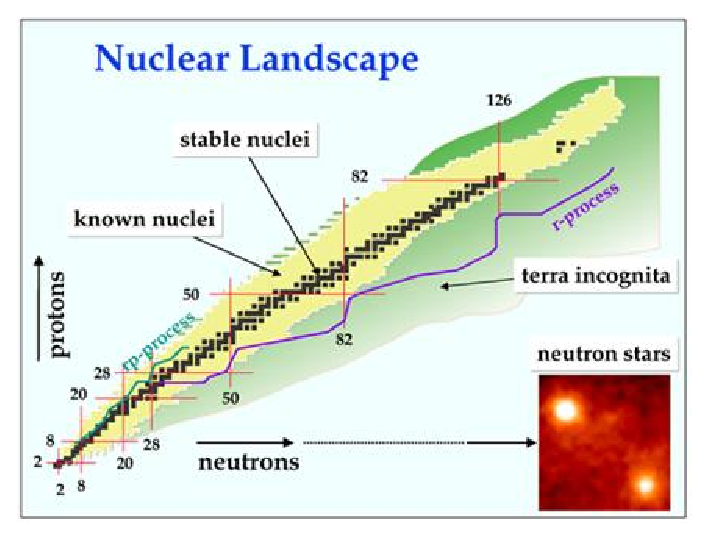
\includegraphics{figs/landscape.eps}} \par}
\end{figure}

Note that:
 \bi 
 \item Not all unstable nuclei are weakly-bound. 
 \item There are weakly-bound nuclei which are not unstable (eg.~deuteron).
 \ei

\end{frame}



% --------------------------------------------------------------------------------------
\slide{Light exotic nuclei: halo nuclei and Borromean systems}

\begin{figure}{\par \resizebox*{0.75\textwidth}{!}
{\includegraphics[angle=-90]{figs/segre.ps}} \par}
\end{figure}

\end{frame}

% --------------------------------------------------------------------------------------
\slide{Light exotic nuclei: halo nuclei and Borromean systems}

\begin{itemize}
\setlength{\itemsep}{11pt}
\gitem{Radioactive nuclei:} they typically decay by $\beta$ emission. \\
{\bf E.g.:}~\nuc{6}{He} $\xrightarrow{\beta ^{-}}$ \nuc{6}{Li} ~~~ ($\tau_{1/2}\simeq $807 ms)

\gitem{Weakly bound}: typical separation energies are around 1 MeV or less.

\gitem{Spatially extended}

\gitem{Halo structure:} one or two weakly bound nucleons (typically neutrons) with a large 
probability of presence beyond the range of the potential.

\gitem{Borromean nuclei:} Three-body systems with no bound binary sub-systems. 

\begin{columns}
\column{0.5\linewidth}
\begin{figure}{\par \resizebox*{0.45\textwidth}{!}
{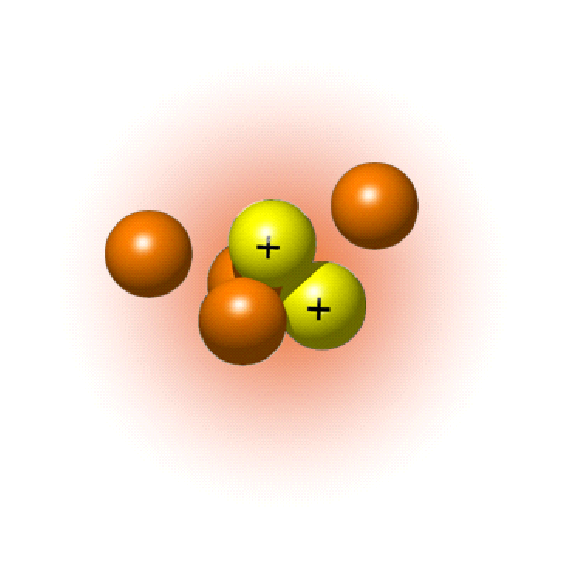
\includegraphics{\images/6He.eps}} \par}
\end{figure}
\column{0.5\linewidth}
\begin{figure}{\par \resizebox*{0.4\textwidth}{!}
{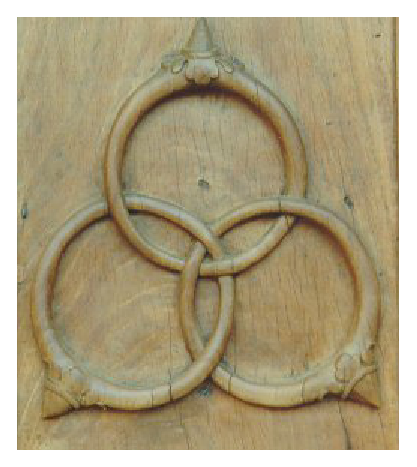
\includegraphics{\images/borromean}} \par}
\end{figure}
\end{columns}
\end{itemize}
\end{frame}





%%%%%%%%%%%%%%%%%%%%%%%%%%%%%%%%%%%%%%%%%%%%%%%%%%%%%%%%
\section{Signatures of weakly-bound nuclei in reaction observables}
%%%%%%%%%%%%%%%%%%%%%%%%%%%%%%%%%%%%%%%%%%%%%%%%%%%%%%%%

\slide{}
\begin{center}
\psframebox[fillcolor=green!10,linecolor=blue,framearc=0.1,fillstyle=solid,framesep=5pt]{
Signatures of weakly-bound nuclei in reaction observables
}%psframe
\end{center} 
\end{frame}

%--------------------------------------
%\slide{Elastic scattering}
%{\bf \brick Let's start from the beginnning $\ldots$ ; Rutherford experiment:}
%\begin{figure}{\par \resizebox*{0.75\textwidth}{!}
%{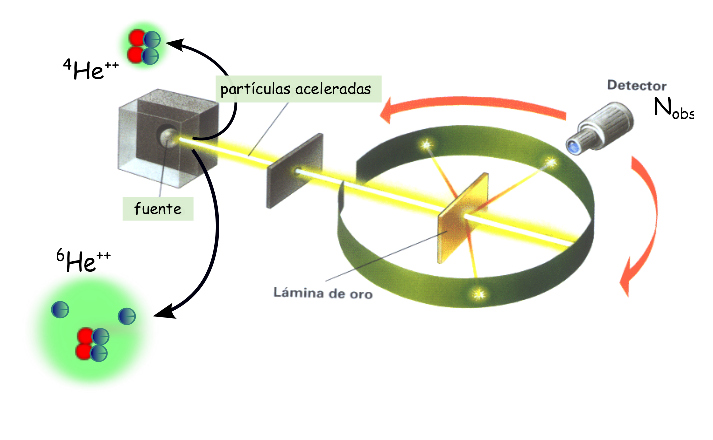
\includegraphics{figs/ruth.eps}} \par}
%\end{figure}
%\end{frame}

%---------------------------------------------
\slide{Elastic scattering: Rutherford experiment...100 years later}
\begin{columns}
\column{0.5\textwidth}
\begin{center}\includegraphics[width=0.8\columnwidth]{figs/he46pb_e19_data.eps}\end{center}
\column{0.5\textwidth}
\begin{center}\includegraphics[width=0.8\columnwidth]{figs/he46pb_e22_data.eps}\end{center}
\end{columns}

\begin{itemize}
\item $^4$He follows Rutherford formula at 19~MeV but not at 22~MeV.
\item $^6$He drastically departs  from Rutherford formula at both energies!
\end{itemize}
\end{frame}


%---------------------------------------------
\slide{Inclusive breakup cross sections}

$$
\psframebox[fillcolor=yellow,linecolor=red,framearc=0.1]{
{\rm ^{6}{He} + ^{208}{Pb} \rightarrow  \alpha + X}
}
$$

\begin{columns}[c]
\column{.5\textwidth}
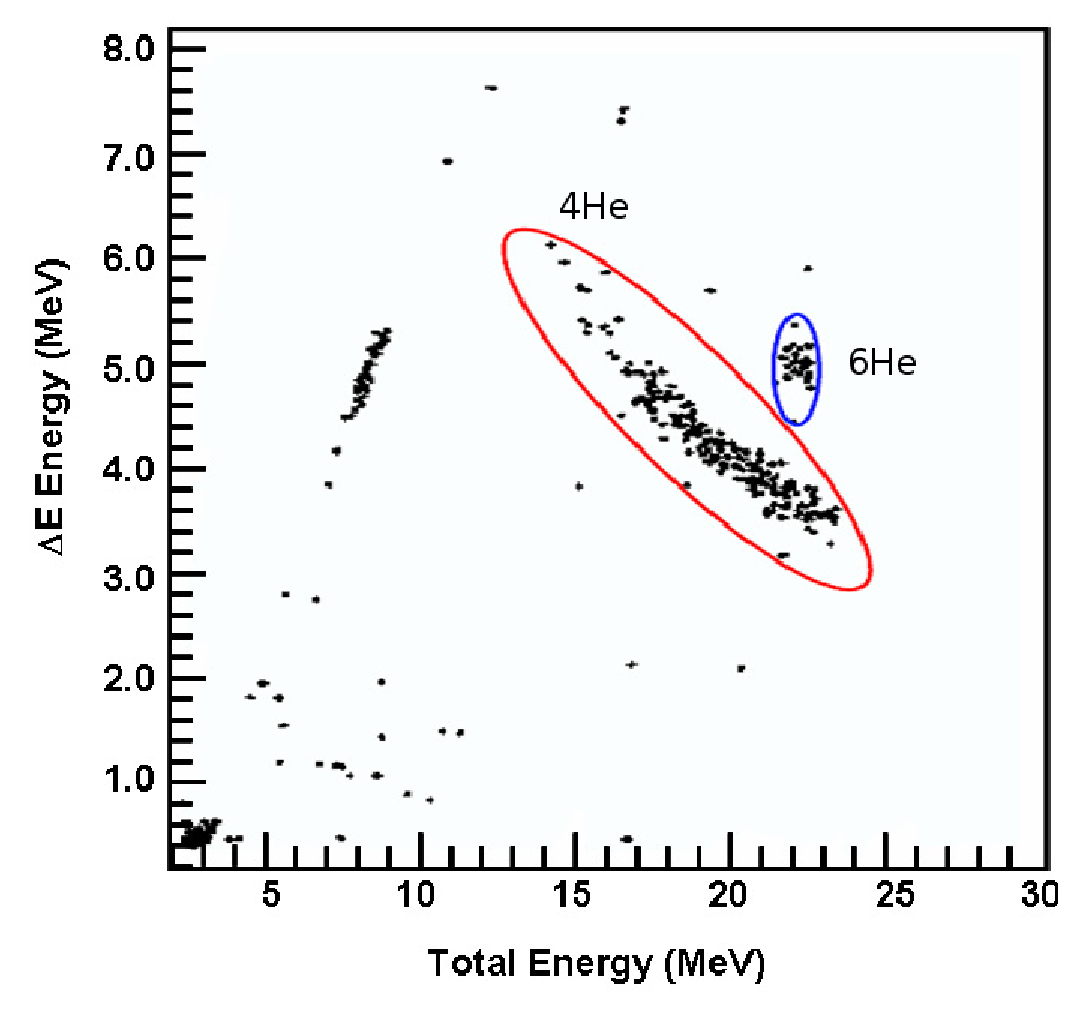
\includegraphics[height=4cm]{\images/bidim-22MeV-new2.eps} 
\column{.5\textwidth}
\includegraphics[height=4cm]{\images/he6pb_e22_pbu_data.eps} 
\end{columns}


%\begin{center}\includegraphics[width=0.55\columnwidth]{\images/he4_he6_ratio_vs_theta.eps}\end{center}

\ding{233}{At large angles, there are more $\alpha$'s than $^{6}$He (elastic) ! } \\
\ding{233}What are the mechanisms behind the $\alpha$ producion and how can we compute it? 

\end{frame}


% --------------------------------------------------------------------------------------
\slide{High-energy interaction cross sections with light targets}

\only<1>{
\ding{32} Interaction cross sections of nuclei on light targets and high energies are proportional to the size of the colliding nuclei.  
%\ding{43} First evidences of the existence of halo nuclei came from reaction cross sections measurements.

\vspace{-0.5cm}

\bc
\column{0.5\linewidth}
$$
\psframebox[fillcolor=yellow,linecolor=red,framearc=0.1]{
\sigma_I \simeq \pi (R_p+R_t)^2
}
$$
\begin{figure}{\par \resizebox*{0.8\textwidth}{!}
{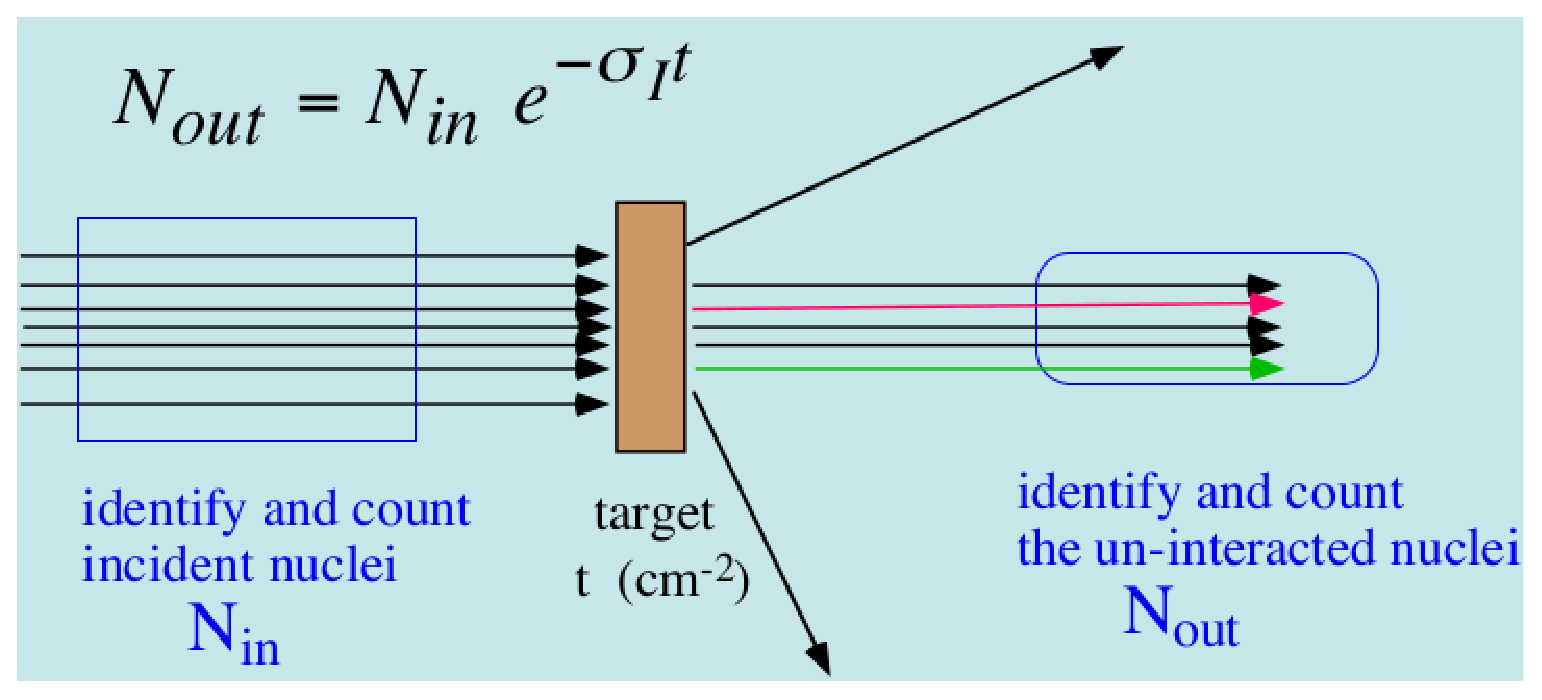
\includegraphics[width=0.95\columnwidth]{\images/interaction_xs.eps}} \par}
\end{figure}
{\small \verde From I.~Tanihata }
\column{0.5\linewidth}
\vspace{0.5cm}
\begin{center}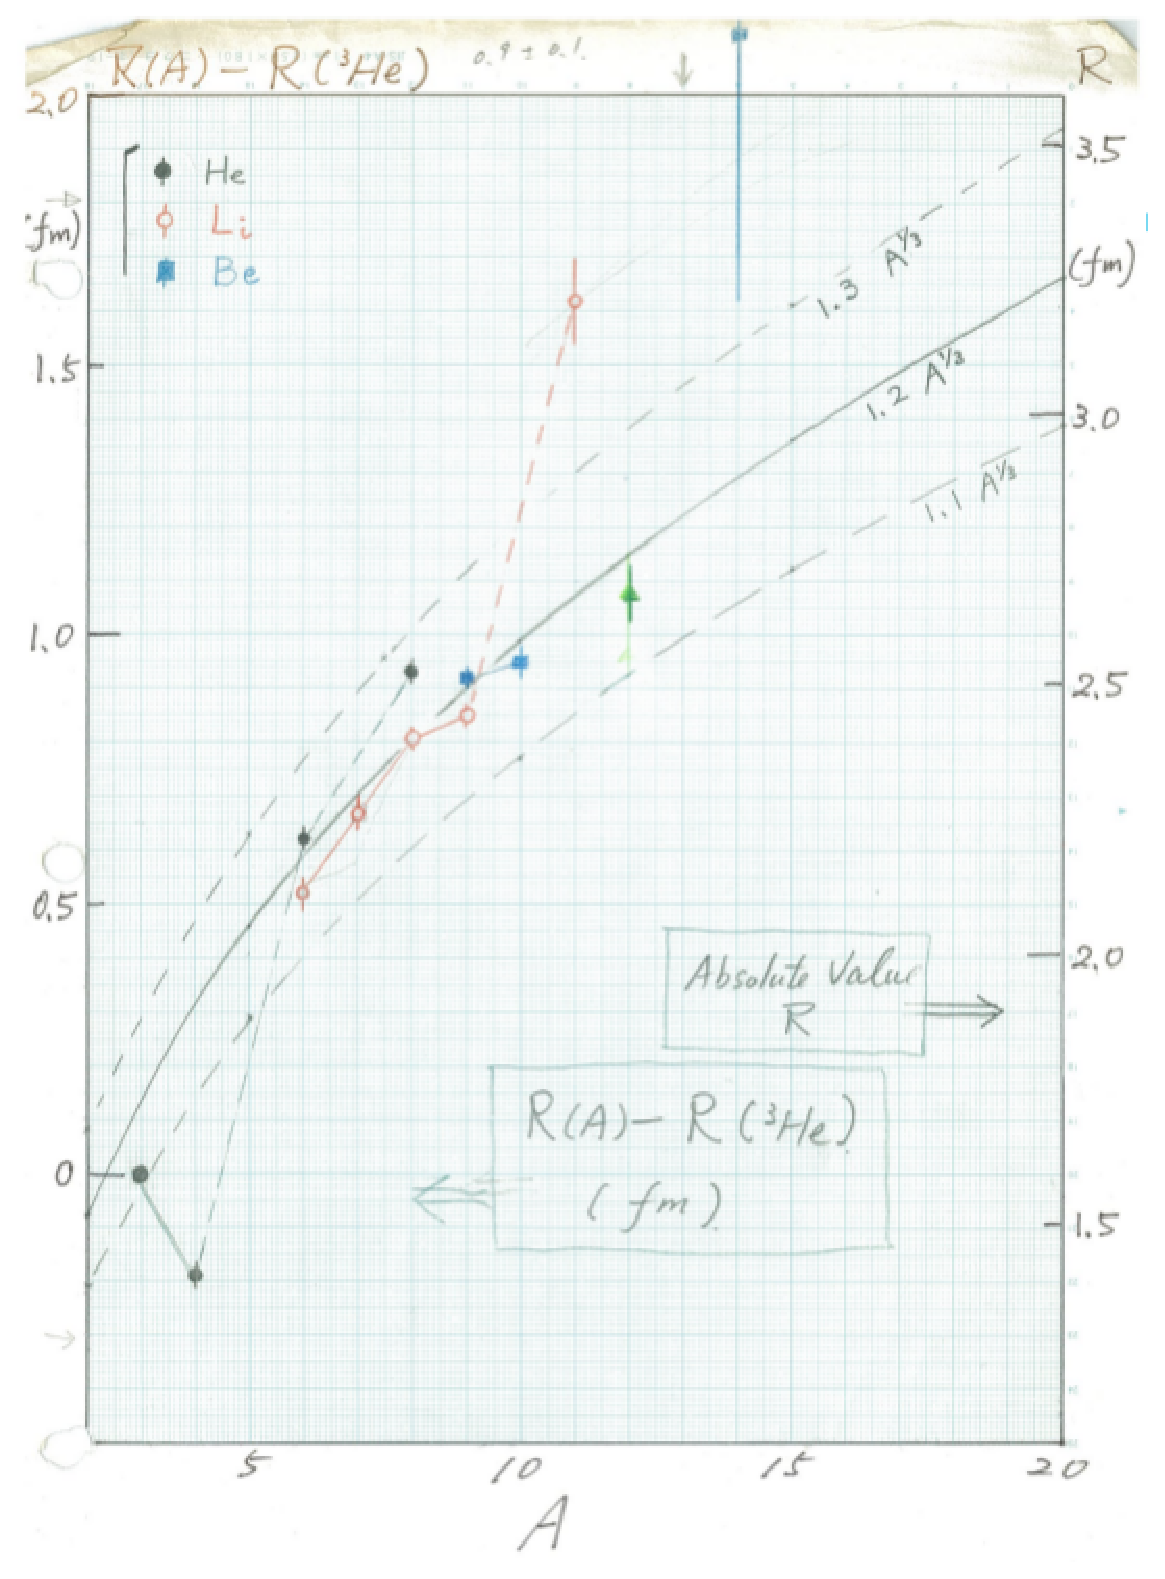
\includegraphics[height=7.0cm]{\images/radios_tanihata_orig.eps}\end{center}
\end{columns}%twocolumn
}%onslide


\only<2>{
\ding{32} Interaction cross sections of nuclei on light targets and high energies (hundreds MeV/nucleon) are proportional to the size of the colliding nuclei.  
%\ding{43} First evidences of the existence of halo nuclei came from reaction cross sections measurements.

\vspace{0.25cm}

\bc
\column{0.6\linewidth}
$$
\psframebox[fillcolor=yellow,linecolor=red,framearc=0.1]{
\sigma_I \simeq \pi (R_p+R_t)^2
}
$$
\begin{figure}{\par \resizebox*{0.5\textwidth}{!}
{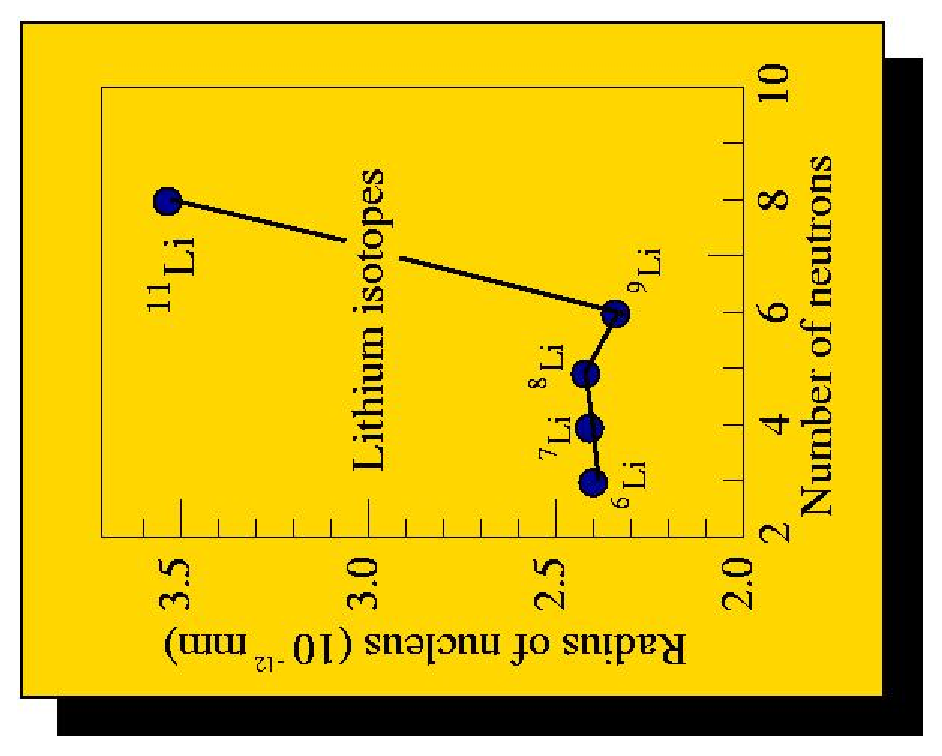
\includegraphics[angle=-90]{\images/liradii.eps}} \par}
\end{figure}
{\small \verde Tanihata {\em et al}, PRL55, 2676 (1985)}
\column{0.4\linewidth}
\vspace{0.5cm}
\begin{center}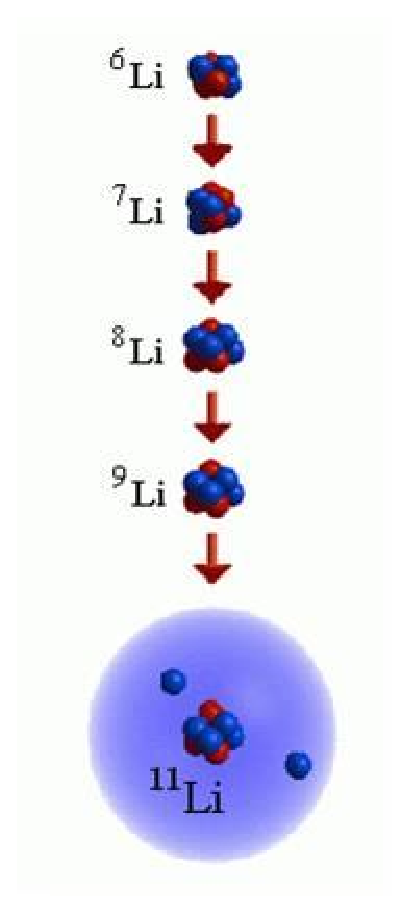
\includegraphics[height=5.0cm]{\images/lithium-isotopes.eps}\end{center}
\end{columns}%twocolumn
}%onslide

\only<3>{
Momentum distributions in breakup reactions
\begin{figure}
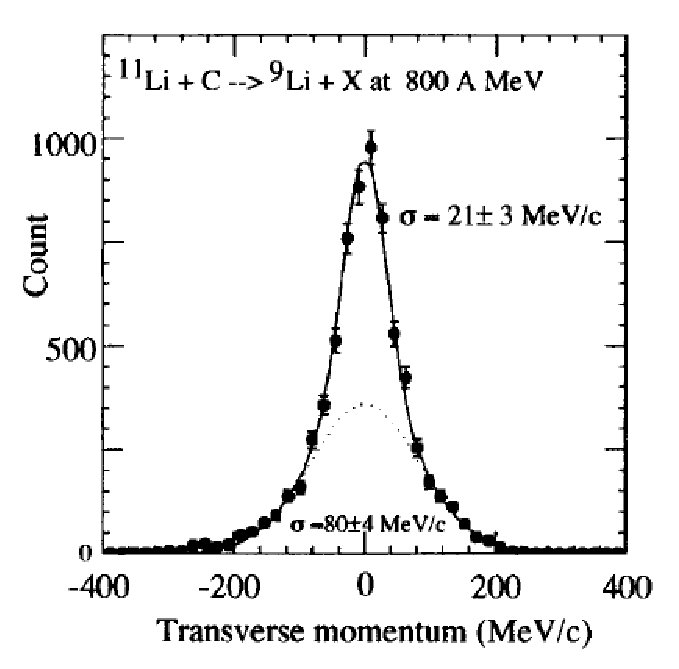
\includegraphics[height=0.6\textheight]{\images/li9momdis.eps}
\end{figure}
\ding{43} {\em \brick A narrow momentum distribution is a signature of  an extended spatial distribuion}
}%onslide

\only<4>{
\begin{figure}
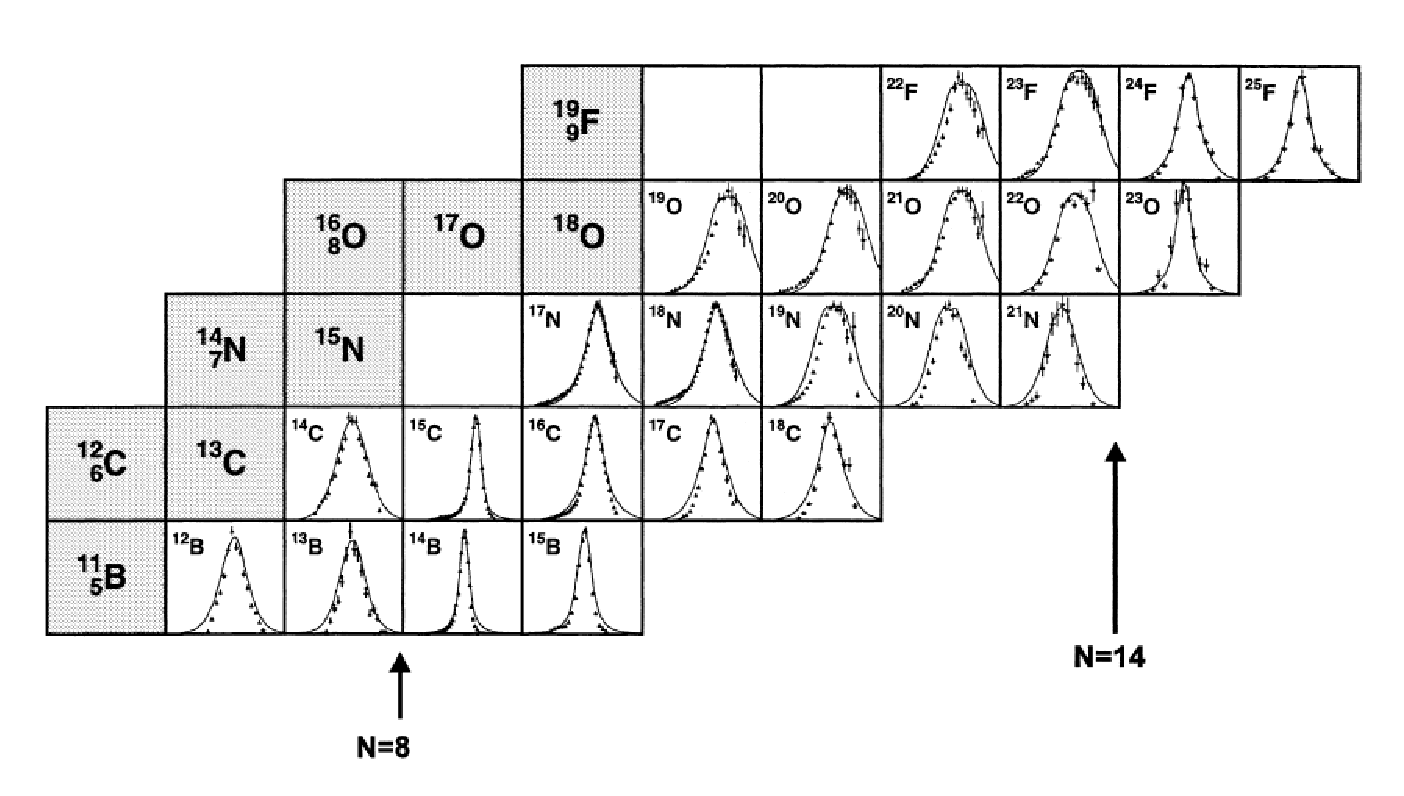
\includegraphics[height=0.7\textheight]{\images/momdis_chart.eps}

\end{figure}
}%only

\end{frame}




\endinput

%----------------------------------
\subsection{Some scattering theory}

\slide{}
\begin{center}
\psframebox[fillcolor=green!10,linecolor=blue,framearc=0.1,fillstyle=solid,framesep=5pt]{
Some scattering theory
}%psframe
\end{center} 
\end{frame}












%--------------------------------------
\section{Modelling reactions}
%--------------------------------------

%----------------------------------
%\subsection{Some scattering theory}

\slide{}
\begin{center}
\psframebox[fillcolor=green!10,linecolor=blue,framearc=0.1,fillstyle=solid,framesep=5pt]{
Modelling nuclear reactions
}%psframe
\end{center} 
\end{frame}


%-----------------------------------------------------------------------------------------
\slide{Why reaction theory is important?}

\begin{itemize}
\setlength{\itemsep}{14pt}
\item Reaction theory provides the necessary framework to extract meaningful {\blue structure} information from measured {\blue cross sections} and also permits the understanding of the {\blue dynamics} of nuclear collisions.


\item The many-body scattering problem is not solvable in general,  so specific models tailored to specific types of reactions are used ({\blue elastic}, {\blue breakup}, {\blue transfer}, {\blue knockout}...)
each of them emphasizing some particular degrees of freedom. 

\item In particular,  exotic nuclei close to driplines are usually weakly-bound and {\blue breakup}  (coupling to the continuum) is  important and must be  taken into account in the reaction model. 

\item {\blue Few-body} models provide an appealing simplification of this complicated problem. 


%\item Even after this simplification, the scattering problem is not solvable in general,

\end{itemize}

\end{frame}


%----------------------------------------
\slide{Direct and compound nucleus processes}

%Example: the d+\nuc{10}{Be} case
\begin{figure}{\par \resizebox*{0.75\textwidth}{!}
{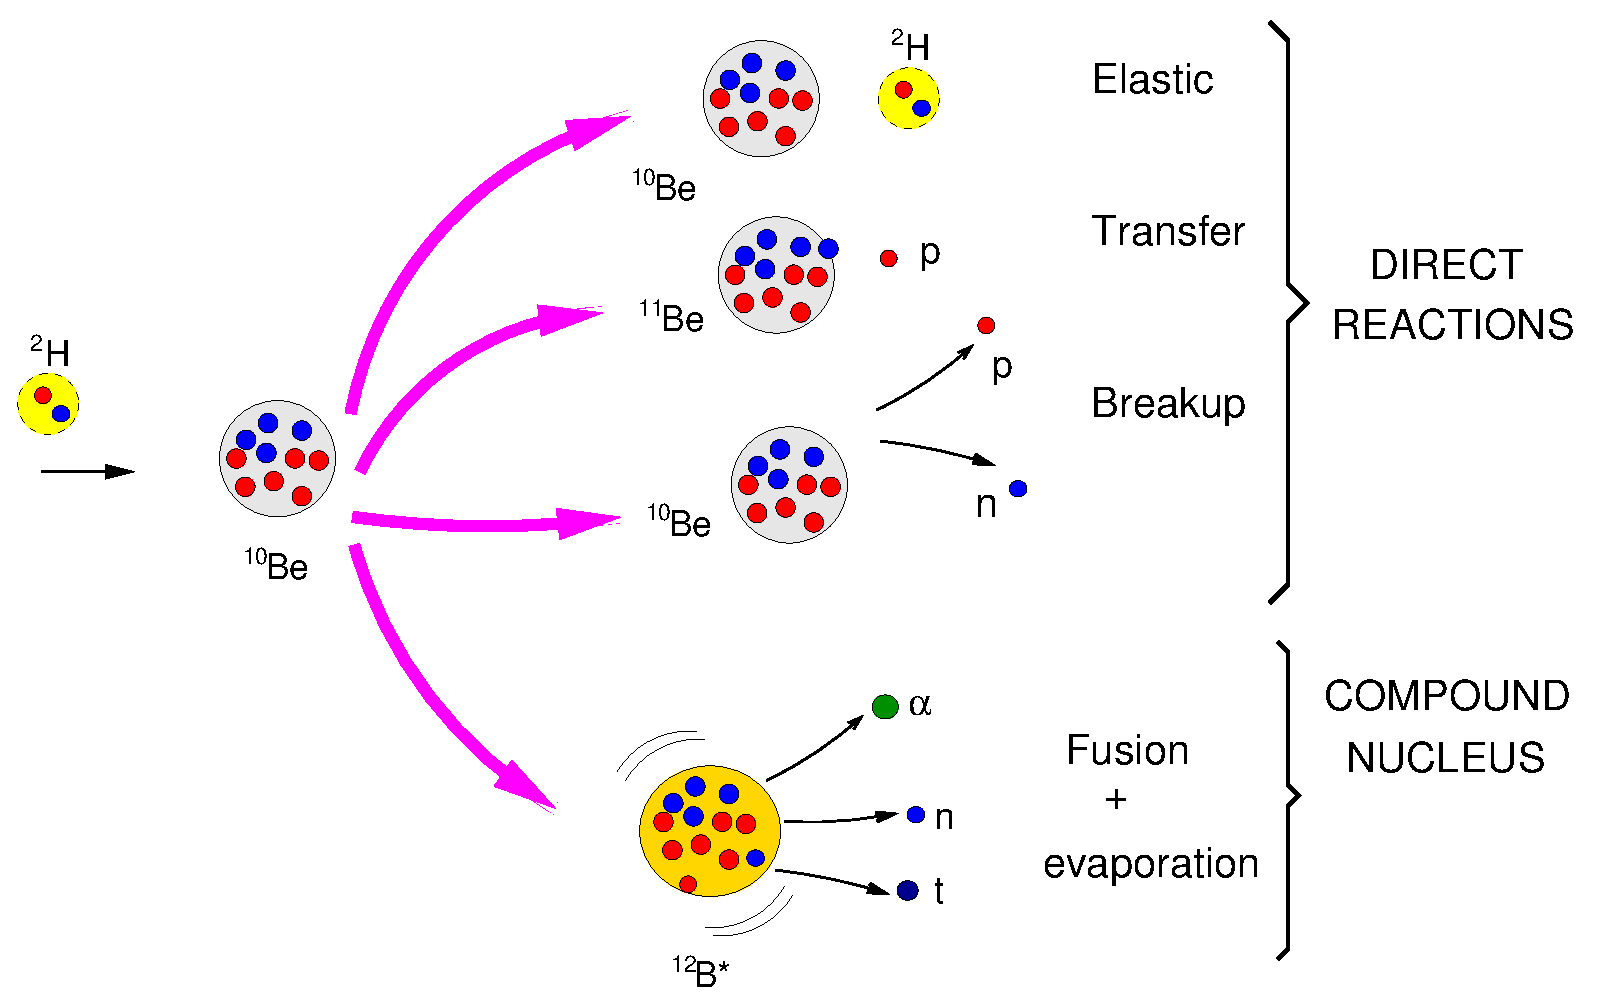
\includegraphics{figs/be10d_chans.eps}} \par}
\end{figure}

\end{frame}





%----------------------------------------
\slide{Direct versus compound reactions}

{\sc \brick Direct:} elastic, inelastic, transfer,\ldots
\begin{itemize}
\setlength{\itemsep}{14pt}
\item ``fast'' collisions (10$^{-21}$~s).
\item only a few modes (degrees of freedom) involved
\item  small momentum transfer
\item angular distribution asymmetric about $\pi/2$ (peaked forward)
\end{itemize}

\vspace{0.5cm}

{\sc \brick Compound:} complete, incomplete fusion.
\begin{itemize}
\setlength{\itemsep}{14pt}
\item many degrees of freedom involved
\item large amount of momentum transfer
\item ``loss of memory''  $\Rightarrow$ almost symmetric distributions forward/backward
\end{itemize}
\end{frame}





%---------------------------------------------------------
\slide{Linking theory with experiments: the cross section}

\let\psgrid\relax
\begin{pspicture}(8,4)
\psgrid
\rput(2,3.0){\rnode{F1}{
\psframebox[fillcolor=red!10,fillstyle=solid,framearc=0.15,linecolor=brick]{
%\psovalbox*[fillcolor=LightBlue,shadow=true]{
 \parbox{3.0cm}{
 \begin{center}
 EXPERIMENT 
 \end{center}

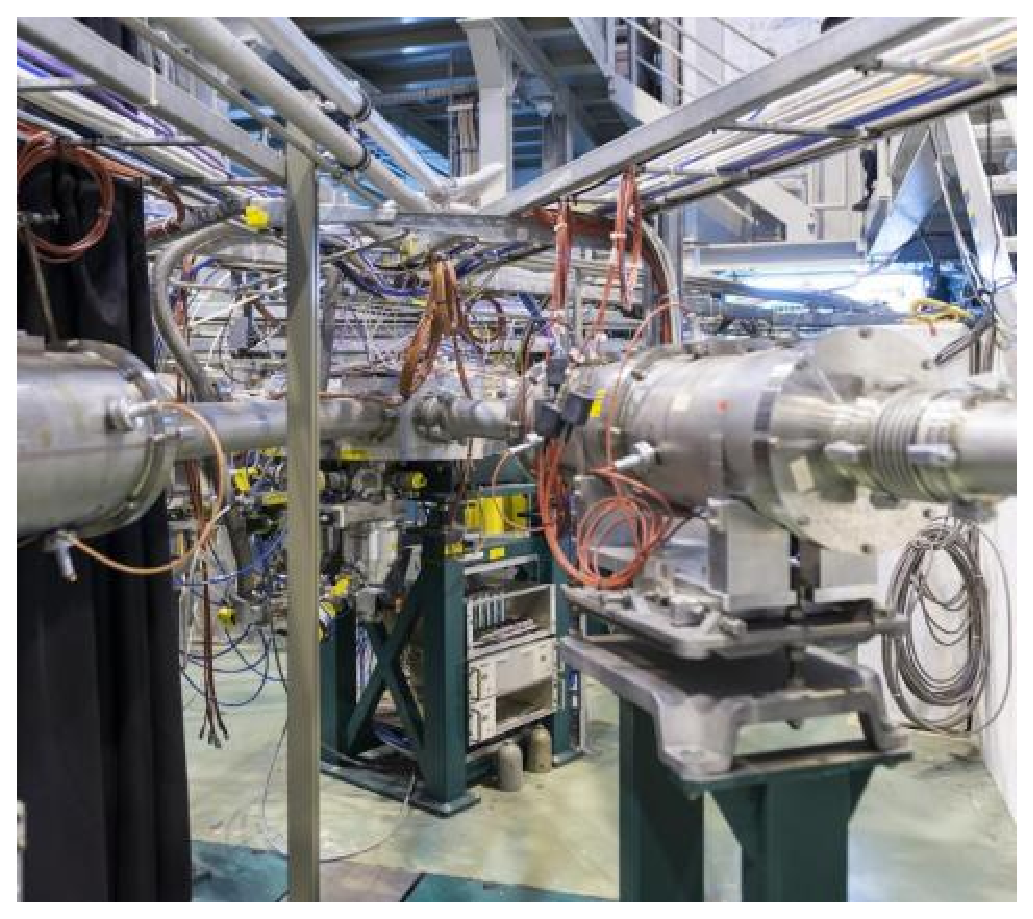
\includegraphics[width=0.25\columnwidth]{figs/isolde.eps}
}%parbox
}}}
\rput(10,3.0){\rnode{F2}{
\psframebox[fillcolor=red!10,fillstyle=solid,framearc=0.15,linecolor=brick]{
%\psovalbox*[fillcolor=LightBlue,shadow=true]{
 \parbox{3.0cm}{
\begin{center} THEORY \\
 ($H \Psi = E \Psi$) 
\end{center}

%  $ \psframebox[fillcolor=green!40,framearc=0.2]{
% H \Psi = E \Psi
% }%psframe
% $

\includegraphics[width=0.22\columnwidth]{figs/computer.eps}
}%parbox
}}}

\pause

\rput(5.5,0.0){\rnode{T1}{\psovalbox*[fillcolor=green!40,shadow=true,fillstyle=solid]{ 
 \parbox{3.0cm}{
CROSS SECTIONS
$$
\frac{d\sigma}{d\Omega}, \frac{d\sigma}{dE}, etc
$$
}
}}}
\end{pspicture}


{\nccurve[linecolor=red,angleA=-90,angleB=180,linewidth=5pt]{->}{F1}{T1}}
{\nccurve[linecolor=red,angleA=-90,angleB=0,linewidth=5pt]{->}{F2}{T1}}
%{\nccurve[linecolor=red,angleA=0,angleB=180]{->}{F3}{T1}}
\end{frame}






\begin{comment}
%---------------------------------------------------------------------------------------
\slide{Experimental cross section}
\begin{itemize}
\item Experimental data consist of cross sections for one or more detected particles

\begin{center}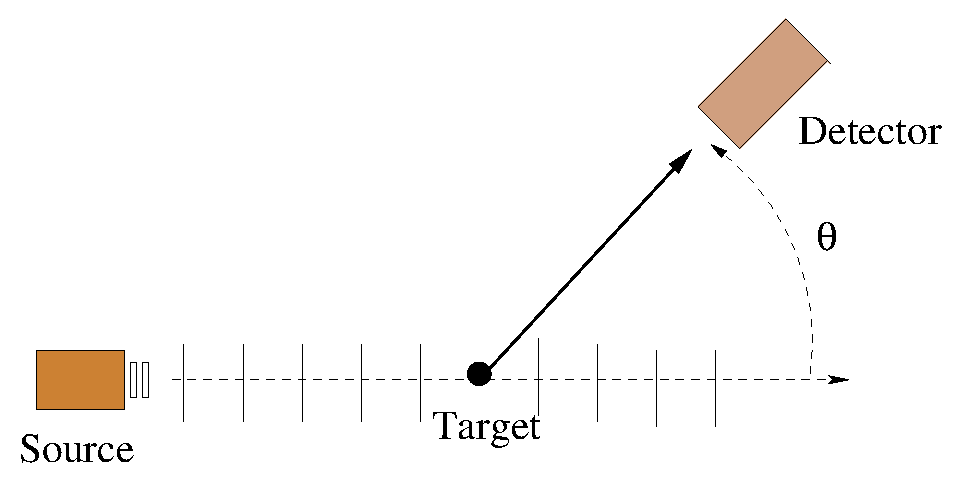
\includegraphics[width=0.35\textwidth]{figs/scattering1.eps}\end{center}

\item Differential cross section:
$$
%\psframebox[fillcolor=green!40,fillstyle=solid,framearc=0.2]{
\psframebox[fillcolor=green!15,linecolor=blue,framearc=0.1,fillstyle=solid]{
\Delta I = I_0 ~ n_t ~ \textcolor{red}{ \frac{d \sigma}{d\Omega} } \Delta \Omega
}%psframe
$$
\begin{itemize}
\item $I_0$: incident particles per unit time
\item $n_t$: number of target nuclei per unit surface
\item $\Delta \Omega$: solid angle of detector
\item $\Delta I$: detected particles per unit time in $\Delta \Omega$
\item $\textcolor{red}{ {d \sigma}/{d\Omega} }$: differential cross section
\end{itemize}
\end{itemize}


\end{frame}
\end{comment}


%---------------------------------------------------------------------------------------
\slide{Experimental cross section}
%\begin{itemize}
%\item Experimental data consist of cross sections for one or more detected particles
\begin{columns}
\column{0.5\textwidth}
\begin{center}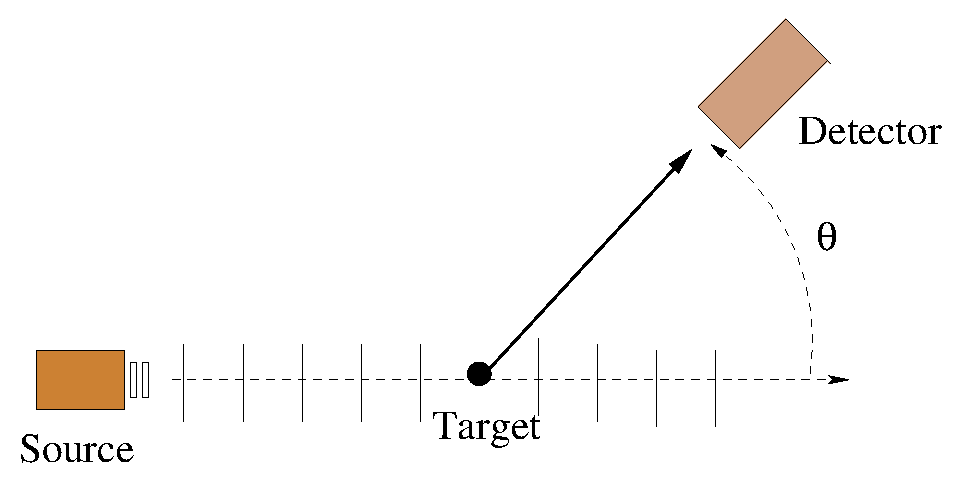
\includegraphics[width=0.8\columnwidth]{figs/scattering1.eps}\end{center}
\column{0.5\textwidth}
$$
%\psframebox[fillcolor=green!40,fillstyle=solid,framearc=0.2]{
\psframebox[fillcolor=green!15,linecolor=blue,framearc=0.1,fillstyle=solid]{
\Delta I = I_0 ~ n_t ~ \textcolor{red}{ \frac{d \sigma}{d\Omega} } \Delta \Omega
}%psframe
$$
\end{columns}

\vspace{0.5cm}
%\item Differential cross section:
% $$
% \psframebox[fillcolor=green!15,linecolor=blue,framearc=0.1,fillstyle=solid]{
% \Delta I = I_0 ~ n_t ~ \textcolor{red}{ \frac{d \sigma}{d\Omega} } \Delta \Omega
% }%psframe
% $$
\begin{itemize}
\item $\Delta I$: detected particles per unit time in $\Delta \Omega$
\item $I_0$: incident particles per unit time
\item $n_t$: number of target nuclei per unit surface
\item $\Delta \Omega$: solid angle of detector
\item $\textcolor{red}{ {d \sigma}/{d\Omega} }$: differential cross section
\end{itemize}
%\end{itemize}

$$
\psframebox[fillcolor=green!15,linecolor=blue,framearc=0.1,fillstyle=solid]{
\frac{d\sigma}{d\Omega} =  \frac{\textrm{flux of scattered particles through $dA= r^2 d\Omega$} }{ \textrm{incident flux} }
}%psframe
$$

\end{frame}






%----------------------------------------------------------------
\slide{Projectile and target internal Hamiltonians}
\begin{itemize}
\item Mass partitions: $\alpha$, $\beta$,$\ldots$
\item {\brick Internal} proj. + target Hamiltonians: $H_\alpha(\xi_\alpha) \equiv H_p(\xi_p) + H_t (\xi_t)$
\item Internal states:
$
[H_\alpha (\xi_\alpha) - \varepsilon_\alpha] \Phi_\alpha (\xi_\alpha)=0 \quad \{\varepsilon_\alpha\}=\textrm{excitation energies}
$
\item Different mass partitions  have different Hamiltonians: $H_\alpha(\xi_\alpha)$,$H_\beta (\xi_\beta)$, etc
\end{itemize}

\resizebox*{0.7\textwidth}{!}{\input{figs/be10d_chans_H.pstex_t}}
%\scalebox{.4}{ \input{figs/be10d_chans_H.pstex_t} }
\end{frame}




%----------------------------------------------
\slide{Model Hamiltonian and model wavefunction}

\begin{block}{Full Hamiltonian}
$$
\psframebox[linecolor=red,framearc=0.1,framesep=5pt]{
H= \hat{T}_\bR + H_p(\xi_p) + H_t(\xi_t) + V(\bR,\xi_p,\xi_t) 
}%psfr
$$
\begin{itemize}
\item $\hat{T}_\bR $: proj.--target kinetic energy
\item $H_p(\xi_p)$: projectile Hamiltonian
\item $H_t(\xi_t)$: target Hamiltonian
\item $V(\bR,\xi_p,\xi_t)$: projectile--target interaction
\end{itemize}
\end{block}

%\begin{block}{Scattering wavefunction}
Time-independent Schrodinger equation:
$$
\psframebox[linecolor=red,framearc=0.1,framesep=5pt]{
[H - E ] \Psi(\bR,\xi_p,\xi_t) = 0
}%psfr
$$
%\end{block}

\end{frame}





%------------------------------------------------------
\slide{Scattering wavefunction}

\begin{center}
%\begin{figure}
\begin{minipage}{0.62\textwidth}
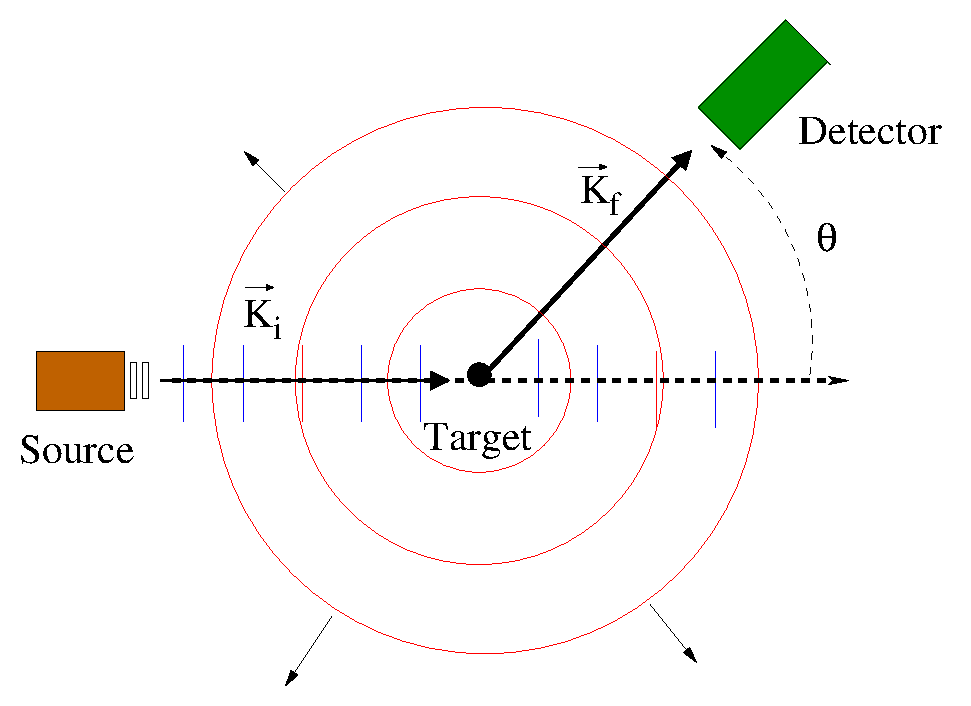
\includegraphics[width=0.75\columnwidth]{figs/scattering.eps}
\end{minipage}
\begin{minipage}{0.35\textwidth}
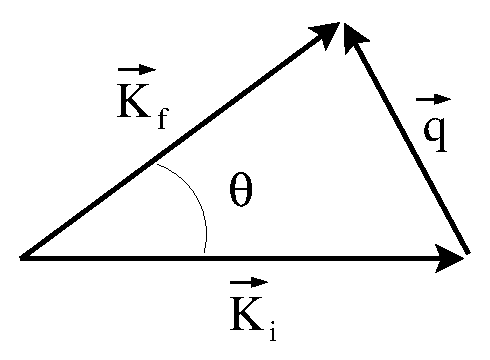
\includegraphics[width=0.6\columnwidth]{figs/transfer_mom.eps}
\end{minipage}
%\caption{\label{fig:scattering} Left: schematic representation of a scattering process. Right: initial, final and transferred momenta.}
%\end{figure}
\end{center}

%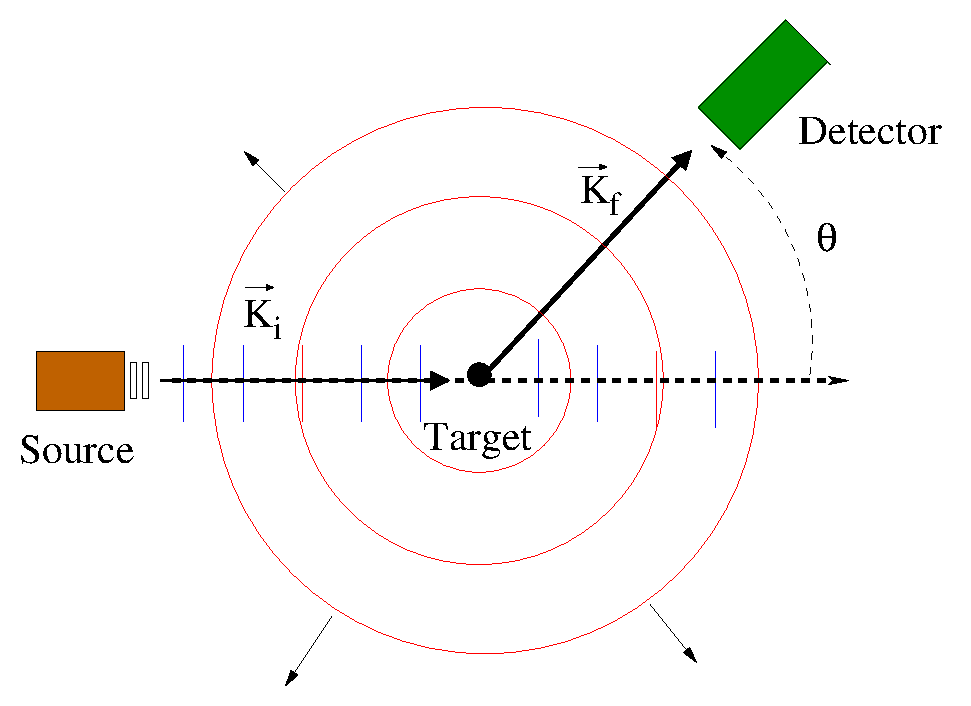
\includegraphics[width=0.5\columnwidth]{figs/scattering.eps}


Among the many mathematical solutions of $ [H - E ] \Psi = 0$ we are interested  in those behaving asymptotically as:

%\parbox{0.9\textwidth}{
$$
%\psframebox[fillcolor=magenta!10,linecolor=red,framearc=0.1,fillstyle=solid,framesep=8pt]{
\psframebox[linecolor=red,fillcolor=orange!10,fillstyle=solid,framearc=0.2,framesep=8pt]{
\Psi^\mathrm{(+)}_{\bK_\alpha} \rightarrow   \Phi_\alpha(\xi_\alpha) e^{i \bK_\alpha \cdot \bR_\alpha} +
 \textrm{(outgoing spherical waves in $\alpha$, $\beta$, $\ldots$)}
}%psframebox
$$
%}%parbox
%}%psframe


%\end{itemize}


\end{frame}


%-----------------------------------------------
\slide{Scattering amplitude and cross sections}

%\begin{center}
%\psframebox[fillcolor=magenta!5,linecolor=red,framearc=0.1,fillstyle=solid,framesep=-8pt]{
\psframebox[linecolor=red,fillcolor=orange!10,fillstyle=solid,framearc=0.2,framesep=-8pt]{
\parbox{0.9\textwidth}{
\begin{align*}
\Psi^\mathrm{(+)}_{\bK_\alpha}   \xrightarrow{R_\alpha \gg}  & \Phi_\alpha(\xi_\alpha) e^{i \bK_\alpha \cdot \bR_\alpha} +  \Phi_\alpha(\xi_\alpha) f_{\alpha,\alpha}(\theta) \frac{e^{i K_\alpha R_\alpha}}{R_\alpha}  & \quad \textrm{(elastic)}
\\
  & +\sum_{\alpha' \neq \alpha} \Phi_{\alpha'}(\xi_\alpha) f_{\alpha',\alpha}(\theta) \frac{e^{i K_{\alpha'} R_\alpha}}{R_\alpha} 
 & \quad \textrm{(inelastic)}
 \\
\Psi^\mathrm{(+)}_{\bK_\alpha}   \xrightarrow{R_\beta \gg}  & \sum_{\beta} \Phi_\beta(\xi_\beta) f_{\beta,\alpha}(\theta) \frac{e^{i K_\beta R_\beta}}{R_\beta} 
 & \quad \textrm{(transfer)}
\end{align*}
}%parbox
}%psframe

\vspace{0.5cm}


%\begin{block}{Cross sections:}
{\bf Cross sections:} 
$$
%\psframebox[fillcolor=magenta!8,linecolor=red,framearc=0.1,fillstyle=solid,framesep=6pt]{
\psframebox[linecolor=red,fillcolor=orange!10,fillstyle=solid,framearc=0.2,framesep=6pt]{
\left ( \frac{d\sigma}{d\Omega} \right)_{\alpha \rightarrow \beta} = \frac{K_\beta}{K_\alpha} \left| f_{\beta,\alpha}(\theta) \right|^2 
}%psr
\quad
E= \frac{\hbar^2 K^2_\alpha}{2 \mu_\alpha} + \varepsilon_\alpha = \frac{\hbar^2 K^2_\beta}{2 \mu_\beta} + \varepsilon_\beta
$$ 
%\end{block}
 {\red $f_{\beta,\alpha}$ } is called {\brick scattering amplitude}

%
\end{frame}

%---------------------------------------------------------
\slide{}
{\bf Ideally, the strategy would be:}
\begin{enumerate}
\item Choose structure model for $H_\alpha(\xi)$
\item Compute $\Psi^\mathrm{(+)}$ by solving $[H-E]\Psi^{(+)}=0$
\item Consider the limit $R \gg$ of $\Psi^\mathrm{(+)}$ 
\item Project it on the desired final state to extract the scattering amplitude:
$$
(\Phi_{\alpha'}(\xi_\alpha) | \Psi^\mathrm{(+)} \rangle = {\red f_{\alpha',\alpha}(\theta)} \frac{e^{i K_{\alpha'} R_\alpha}}{R_\alpha} 
$$ 
\end{enumerate}

\pause
{\bf But...}
\begin{itemize}
\item $\Psi$ is a solution of a complicated many-body problem, not solvable in most cases. 
\item The number of accesible channels and states can be huge. 
\end{itemize} 

\vspace{0.5cm}

\ding{233}{\it So, in practice, we will be happy with an approximation of {\red $\Psi$} (or ${\red f(\theta)}$) in a restricted modelspace} 
\end{frame}

%---------------------------------------------------------





\subsection{Feshbach formalism: P and Q spaces}
%---------------------------------------------------------
\slide{Defining our model space: Feshbach formalism}

\begin{itemize}
\item Divide the full space into two groups: \textcolor{red}{P} and {\red Q}
\begin{itemize}
\item[\ding{233}] {\red P}: channels of interest
\item[\ding{233}] {\red Q}: remaining channels 
 \end{itemize}

\item  Write $\Psi = \Psi_P + \Psi_Q$

\begin{center}
%\psframebox[fillcolor=magenta!5,linecolor=red,framearc=0.1,fillstyle=solid,framesep=-7pt]{
\psframebox[linecolor=red,fillcolor=orange!10,fillstyle=solid,framearc=0.2,framesep=-7pt]{
\parbox{0.4\textwidth}{
\begin{align*}
(E-H_{PP}) \Psi_P & = H_{PQ} \Psi_Q  \\
(E-H_{QQ}) \Psi_Q & = H_{QP} \Psi_P 
\end{align*}
}%parbox
}%psframe
\quad ( $H_{PP}=P H P $,  $H_{PQ}=P H Q $,  etc )
\end{center}

\item Eliminate (formally) $\Psi_Q$:
$$
%\psframebox[fillcolor=magenta!5,linecolor=red,framearc=0.1,fillstyle=solid,framesep=5pt]{
\psframebox[linecolor=red,fillcolor=orange!10,fillstyle=solid,framearc=0.2,framesep=5pt]{
\underbrace{ \left [H_{PP} + H_{PQ} \frac{1}{E- H_{QQ} + i \epsilon} H_{QP}  \right ] }_{H_\mathrm{eff} } \Psi_P = E \Psi_P 
}%psframe
$$

\item $H_\mathrm{eff}$ too complicated (complex, energy dependent, non-local) $\Rightarrow$  needs to be replaced by a simpler Hamiltonian: 
$$
H_\mathrm{eff} \longrightarrow H_\mathrm{model} \quad \textrm{(complex, energy dependent)}
$$ 

\end{itemize}
\end{frame}


%-------------------------------------------
\slide{Strategy for reaction calculaions}

We need to make a choice for:
\bigskip

\begin{enumerate}
\setlength{\itemsep}{14pt}
\item {\brick Modelspace:} what channels are to be included?

\item {\brick Structure model:} for projectile and target
\item[] (Microscopic, collective, cluster...)

\item {\brick Reaction formalism}

\end{enumerate}

\end{frame}


%---------------------------------------
\subsection{Defining the modelspace}
\slide{Choice of the modespace: the d+\nuc{10}{Be} example}

\begin{figure}{\par \resizebox*{0.7\textwidth}{!}
{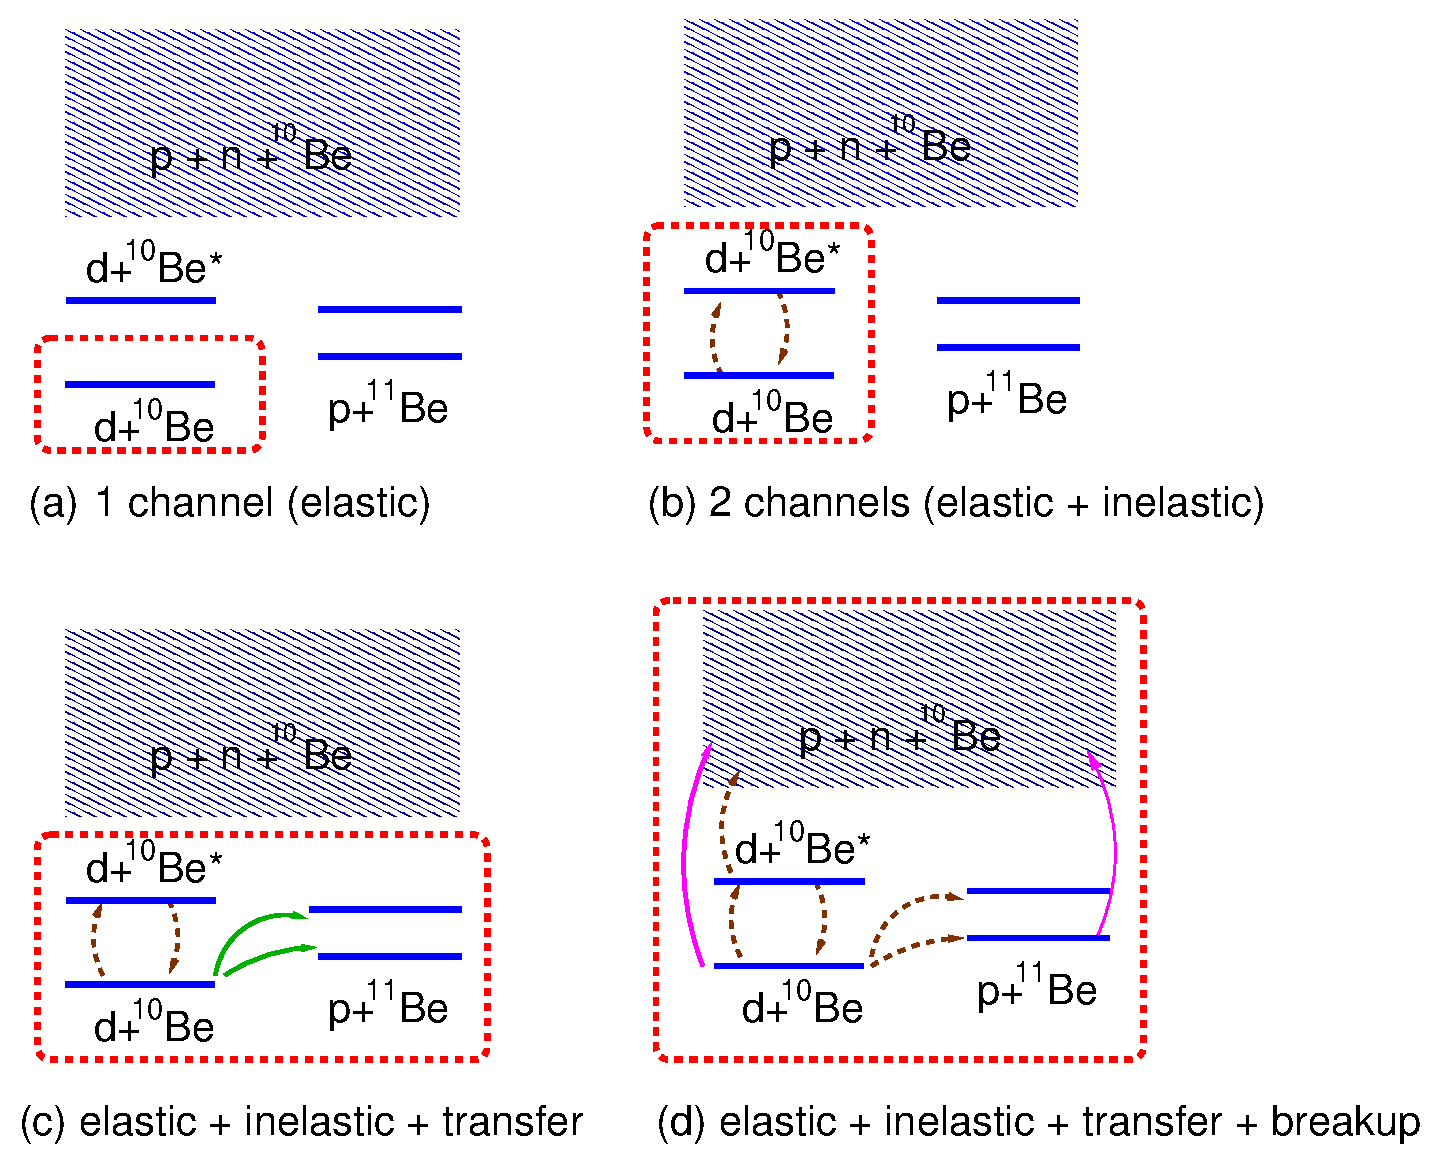
\includegraphics{figs/be10dp_channels.eps}} \par}
\end{figure}

\end{frame}




%------------------------------------------------------
\slide{Choice of structure model: from the many-body problem to the few-body picture}

\scriptsize
\begin{center}
\begin{pspicture}(10,6)
%\psgrid

\visible<1->{
 % --------------------------- MIC CORE ------------------------------------- %  
\rput(4,6){
   \psframebox[linewidth=0,shadow=true,fillcolor=green!25,fillstyle=solid]{%
    \scriptsize Microscopic models 
   }%psframe
   }%rput

\rput(1,5){
  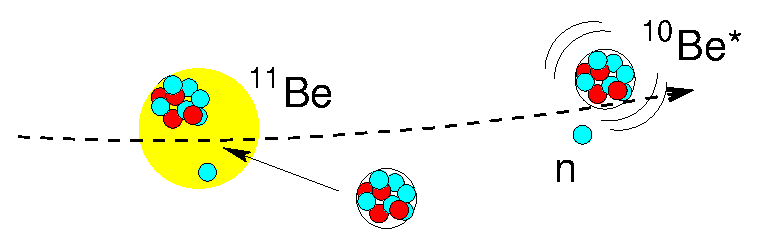
\includegraphics[height=1.25cm]{\images/be11t_mic.eps} 
   }%rput    

\rput(8,5){
   \parbox{0.8\columnwidth}{
    \begin{itemize}    
%    \item[\ding{52}] Achieved for 2-body (CDCC) 
    \item[\ding{52}] Fragments described microscopically
    \item[\ding{52}] Realistic NN interactions (Pauli properly accounted for) 
    \item[\ding{54}] Numerically demanding / not simple interpretation.

    \end{itemize}
    }%parbox
    }%rput
}%visible

 % --------------------------- INERT CORE ------------------------------------- %  
\visible<2->{
\psline[linecolor=orange!40,linewidth=4pt]{<->}(10.7,0)(10.7,6.0)
\rput{-90}(11.,1.5){Few-body}
\rput{-90}(11.,5.0){Many-body}

\rput(4,1.3){
   \psframebox[linewidth=0,framearc=0.2,shadow=true,fillcolor=green!25,fillstyle=solid]{
    Inert cluster models
   }%psframe
   }%rput

\rput(8,0.1){
   \parbox{0.8\columnwidth}{
    \begin{itemize}
%    \item[\ding{54}] Ignores core-excitation admixtures and core transitions.
    \item[\ding{54}] Ignores cluster excitations (only few-body d.o.f).
    \item[\ding{54}] Phenomenological inter-cluster interactions (aprox.~Pauli). 
    \item[\ding{52}] Exactly solvable (in some cases).
    \item[\ding{52}] Achieved for 3-body and 4-body (eg.~coupled-channels, Faddeev).
    \end{itemize}
    }%parbox
    }%rput

\rput(1,0.2){
  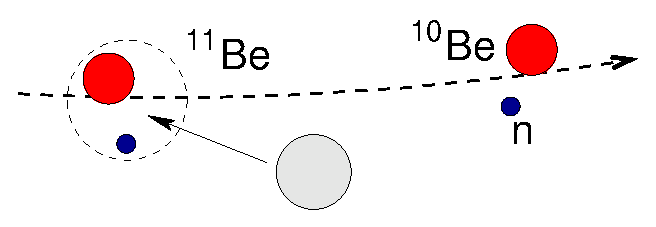
\includegraphics[height=1.25cm]{\images/be11t_inert.eps} 
   }%rput    
}%visible

\visible<3->{
 % --------------------------- CORE EXC ----------------------------------------- % 
\rput(4,3.6){
   \psframebox[linewidth=0,framearc=0.2,shadow=true,fillcolor=green!25,fillstyle=solid]{
    \scriptsize Non-inert-core few-body models   
   }%psframe
   }%rput

\rput(1,2.6){
  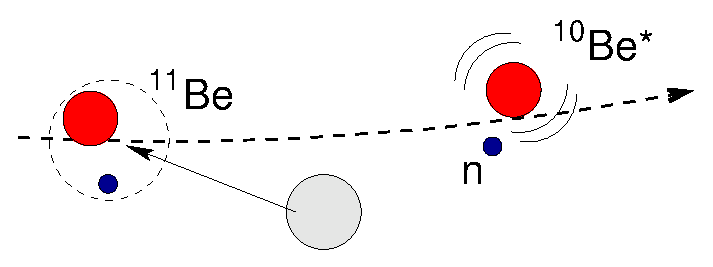
\includegraphics[height=1.25cm]{\images/be11t_corex.eps} 
   }%rput    

\rput(8,2.6){
   \parbox{0.8\columnwidth}{
    \begin{itemize}    
    \item[\ding{52}] Few-body + some relevant collective d.o.f. 
%    \item[\ding{52}] Core excitation within collective model.
    \item[\ding{52}] Pauli approximately accounted for.
    \item[\ding{52}] Achieved for 3-body problems (coupled-channels, Faddeev).    
    \end{itemize}
    }%parbox
    }%rput

}%visible

\end{pspicture}
\end{center}

\end{frame}

\endinput




%-----------------------------------------------------------------------------------------
\slide{}
\begin{center}
\psframebox[fillcolor=green!10,linecolor=blue,framearc=0.1,fillstyle=solid,framesep=5pt]{
Inert-core models: the CDCC method example
}%psframe
\end{center} 
\end{frame}


%%%%%%%%%%%%%%%%%%%%%%%%%%%%%%%%%%%%%%%%%%%%%%%%%%%%%%%%%%%%%%%%%%%%%%%%%%%%%%%%%%%%%%%%%%%%%%%%%%%%%%%%%%%%%%%%%%%%


%---------------------------------------------------------
\slide{Linking theory with experiments: the cross section}


\visible<1>{
\rnode{F1}{
\rput(0.2\columnwidth,0.35\textheight){
\psframebox[fillcolor=red!10,fillstyle=solid,framearc=0.15]{
 \parbox{5cm}{
{\blue \scriptsize \centering EXPERIMENT}
 \begin{center}{\brick \scriptsize Eg:~Spectroscopic factors \\ (knockout vs transfer reactions)} 
 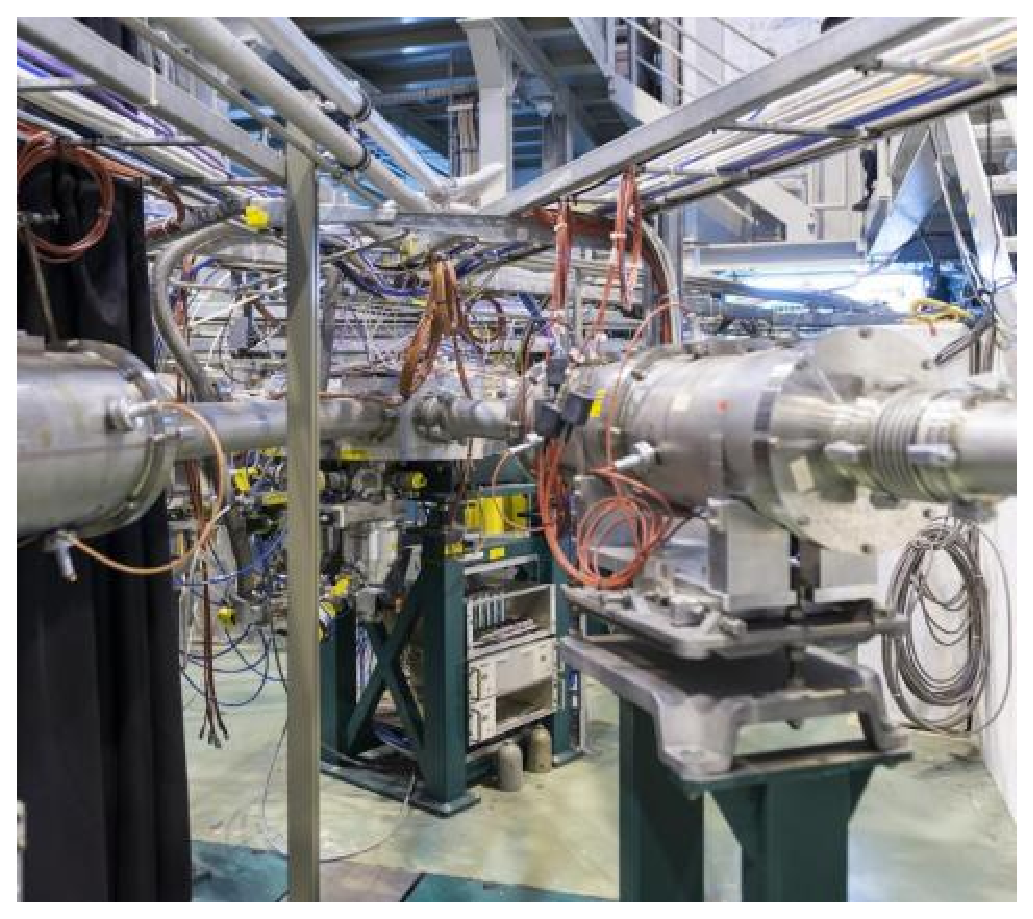
\includegraphics[width=3.0cm,framearc=0.2]{figs/isolde.eps} \\
 \end{center}
  }%parbox
 }%psframe
}%rput
}%rnode
}%visible

\end{frame}



\slide{}
\begin{picture}(0,0)%
\includegraphics{figs/be10d_chans_H.pstex}%
\end{picture}%
\setlength{\unitlength}{3947sp}%
%
\begingroup\makeatletter\ifx\SetFigFont\undefined%
\gdef\SetFigFont#1#2#3#4#5{%
  \reset@font\fontsize{#1}{#2pt}%
  \fontfamily{#3}\fontseries{#4}\fontshape{#5}%
  \selectfont}%
\fi\endgroup%
\begin{picture}(9040,5643)(247,-5589)
\end{picture}%

\end{frame}




\slide{}
\let\psgrid\relax
\begin{pspicture}(8,4)
\psgrid
\rput(1,1){\rnode{F1}{\psovalbox*[fillcolor=LightBlue,shadow=true]{Deformation}}}
\rput(1,1.5){+}
\rput(1,2.2){\rnode{F2}{\psovalbox*[fillcolor=LightBlue,shadow=true]{Pairing}}}
\rput(1,2.8){+}
\rput(1,3.4){\rnode{F3}{\psovalbox*[fillcolor=LightBlue,shadow=true]{Weak binding}}}

\rput(7.5,2.2){\rnode{T1}{\psovalbox*[fillcolor=green!40,shadow=true,fillstyle=solid]{ 
 \parbox{5cm}{
\begin{itemize}
\small
\item How to combine them consistently in {\bf structure}?  
\item How do these effects show  up  in {\bf reactions}?
\end{itemize}
}
}}}
\end{pspicture}

{\nccurve[linecolor=red,angleA=0,angleB=180]{->}{F1}{T1}}
{\nccurve[linecolor=red,angleA=0,angleB=180]{->}{F2}{T1}}
{\nccurve[linecolor=red,angleA=0,angleB=180]{->}{F3}{T1}}
\end{frame}






%%%%%%%%%%%%%%%%%%%%%%%%%%%%%%%%%%%%%%%%%%%%%%%%%%%%%%
\section{Single-channel scattering: the optical model}
%%%%%%%%%%%%%%%%%%%%%%%%%%%%%%%%%%%%%%%%%%%%%%%%%%%%%%
\subsection{Optical model formalism}

\slide{Single-channel scattering: optical model potential}

\begin{itemize} 
\item {\red P} space represents just the ground state of projectile and target 
\item Wavefunction:
$$ \Psi = \underbrace{\Psi_P}_{\textrm{elastic}} + \underbrace{\Psi_Q}_{\textrm{non-elastic}} $$


\item Schrodinger equation in modelspace:
$$
\psframebox[fillcolor=magenta!5,linecolor=red,framearc=0.1,fillstyle=solid,framesep=5pt]{
 \left [T + H_\alpha (\xi_\alpha) + \rnode{F1}{ {\cal V} }  \right ] \Psi_P = E \Psi_P 
% \left [T + H_\alpha (\xi_\alpha) + \rnode{F1}{ \cal V} }  \right ] \Psi_P = E \Psi_P 
}%psframe
$$


$$
\rnode{T2}{
\psframebox[fillcolor=magenta!5,linecolor=red,framearc=0.1,fillstyle=solid,framesep=5pt]{
\rnode{T1}{ {\cal V} }=  \underbrace{ V_{PP} }_{ \textrm{Bare interaction}  } 
% {\cal V} =  \underbrace{ V_{PP} }_{ \textrm{Bare interaction}  } 
           +\underbrace{ V_{PQ} \frac{1}{E- H_{QQ} + i \epsilon} V_{QP} }_{  \textrm{``Polarization'' potential} } 
\equiv V_\mathrm{bare} + V_\mathrm{pol}
}%psframe
}%node
$$

\item ${\cal V} $ too complicated $\Rightarrow$ usually replaced by some phenomenological (complex) potential \textcolor{blue}{$U(\bR)$}  

\end{itemize}

{\nccurve[linecolor=blue,angleA=-90,angleB=90]{->}{F1}{T1}}

\end{frame}





%-------------------------------------------------
\slide{Microscopic folding model for ${\cal V}$  }
%-------------------------------------------------

Start from some (effective) nucleon-nucleon potential $v_{NN}$ (JLM, M3Y, etc):


\begin{enumerate}
\gitem{Single-folding potential:}

\begin{columns}
\column{0.6\textwidth}
$$
V(\bR) = \int \rho_t(\bs_t) v_{NN}(|\bR - \bs|) d\bs
$$
\hspace{1cm} \ding{43} $\rho_t(\bs_t)$=target g.s.~density.

\column{0.4\textwidth}
 \begin{center}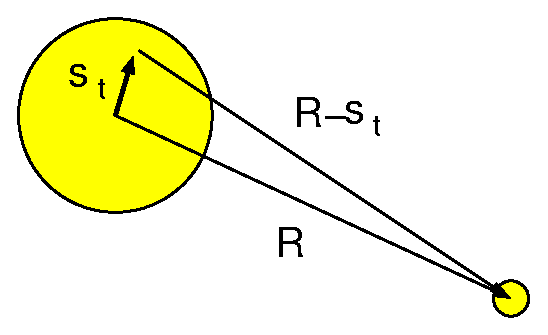
\includegraphics[width=0.65\columnwidth]{figs/singlefold.eps}\end{center}
\end{columns}

\gitem{Double-folding potential:}
\begin{columns}
\column{0.6\textwidth}
$$
V(\bR) = \int \rho_p(\bs_p) \rho_t(\bs_t) v_{NN}(|\bR +\bs_p- \bs_t|) d\bs_p d\bs_t
$$
%\item[\ding{233}] $\rho(s)$=g.s.~density of target.

\column{0.4\textwidth}
 \begin{center}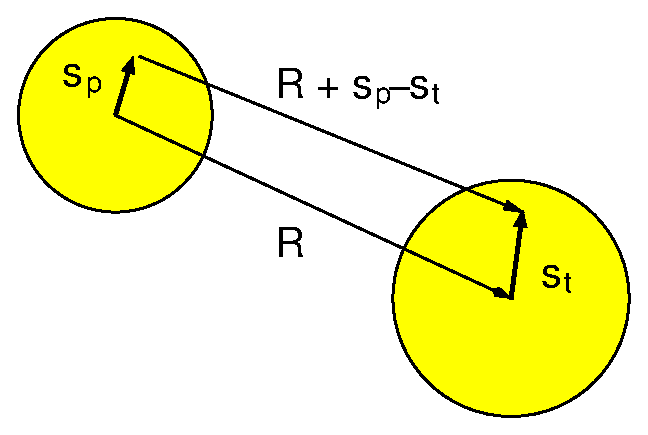
\includegraphics[width=0.65\columnwidth]{figs/doublefold.eps}\end{center}
\end{columns}
\end{enumerate}

\psframebox[fillcolor=blue!10,fillstyle=solid,framearc=0.2,framesep=2pt]{
\parbox{0.95\columnwidth}{%
\small
\bi
\item[\ding{233}] If $\rho_p$ and $\rho_t$ are g.s.\ densities, $V(\bR)$ accounts only for the bare potential ($V_{PP}$) (P-space part) and ignores the effect of non-elastic channels.
\item[\ding{233}] A model for $V_\mathrm{pol}$ must be supplied.
\item[\ding{233}] If  $v_{NN}$ is real, $V(\bR)$ is also real.
\ei
}}

\end{frame}


% ---------------------------------------------------------------------------
\slide{Phenomenological optical model}

{\brick Effective potential:} ${\cal V} \approx U(R)= U_\mathrm{nuc}(R) +  U_\mathrm{coul}(R) $

%\bigskip


\begin{itemize}
 \setlength{\itemsep}{10pt}
\item {\blue Coulomb potential:} charge sphere distribution

\begin{displaymath}
\psframebox[fillcolor=yellow,linecolor=red,framearc=0.1]{
U_\mathrm{coul}(R)=\left\{ \begin{array}{ll}
\frac{Z_1 Z_2 e^2}{2 R_c} \left( 3- \frac{R^2}{R_c^2}\right) & \textrm{if $R \leq R_c$} \\
\frac{Z_1 Z_2 e^2}{R}  & \textrm{if $R \geq R_c$} 
\end{array} \right .
}%psframebox
\end{displaymath}

\item {\blue Nuclear potential (complex):} Eg.~Woods-Saxon parametrization

\begin{equation}
\nonumber
\psframebox[fillcolor=yellow,linecolor=red,framearc=0.1]{
U_\mathrm{nuc}(R)=V(r) + i W(r) = -\frac{V_0}{1+\exp\left(\frac{R-R_0}{a_0}\right)}- i~\frac{W_0}{1+\exp\left(\frac{R-R_i}{a_i}\right)}
}%psframebox
\end{equation}

\ding{233} Popular parametrization: $R_0= r_0 (A_p^{1/3} + A_t^{1/3})$ \quad ($r_0$=reduced radius)

\medskip

\ding{233} For ``normal'' nuclei:  
\begin{itemize}
\item $r_0 \approx r_0  \sim 1.1-1.4$~fm
\item $a_0 \approx a_i \sim 0.5-0.7$~fm
\end{itemize}


\end{itemize}
\end{frame}
%----------------------------------------------------------------------------




% -------------------------------------------------------------------------
\slide{Elastic scattering within the optical model}
%\textcolor{blue}{How does one describe the motion of a particle in quantum mechanics?}

\begin{itemize}
\setlength{\itemsep}{12pt}
\item {\verde Effective Hamiltonian}: $$H = T_{\bR} + H_\alpha(\xi_\alpha) + U(\bR) \quad \quad (U(\bR)~ \textrm{complex!}) $$

\item {\verde $U(\bR)$ independent of $\{ \xi_\alpha \}$ } % $\Rightarrow$ $\Psi^{(+)}_{\bK}(\bR,\xi_\alpha)= $\chi^{}  
$$
\Psi^{(+)}_{\bK}(\xi_\alpha,\bR) = \Phi_{0}(\xi_\alpha) \chi^{(+)}_{0}(\bK,\bR)
$$

%\item[] {\blue $U(R)$}: optical model $\Rightarrow$ effective projectile-target interaction

%\begin{equation}
%H = T(\vec r) + U(r) 
%\nolabel
%\end{equation} 
%\item {\verde Schr\"odinger equation}: $[H-E]\Psi^{+}_{\bK}(\bR)=0$
\item {\verde Schr\"odinger equation}:
$$
\psframebox[fillcolor=magenta!5,linecolor=red,framearc=0.1,fillstyle=solid,framesep=5pt]{ 
[T_{\bR} + U(\bR) -E_\alpha] \chi^{(+)}_{0}(\bK,\bR) =0
}%psframe
\quad \quad (E_\alpha= E- \varepsilon_\alpha = \frac{\hbar^2 K^2}{2\mu}) $$

%\begin{equation}
%\nolabel
%(H-E)\Psi(\vec r)=0
%\end{equation}
\item {\verde Boundary condition:}

$$
\chi^{(+)}_{0}(\bK, \bR)  \rightarrow e^{i \bK \cdot \bR} + 
                    f(\theta) \frac{e^{i KR }}{R}                  
$$

\end{itemize}

\end{frame}





%---------------------------------------------------------------------------------
\slide{Partial wave decomposition}

\begin{itemize}
\item {\verde For a central potential ($U(\bR) = U(R)$):} 
$$
%\chi^{(+)}_0 (\bK,\bR) =  \sum_{\ell m } C_{\ell,m} \frac{\chi_{\ell}(K,R)}{R}  Y_{\ell m}(\hat{R}) 
%\psframebox[fillcolor=magenta!5,linecolor=red,framearc=0.1,fillstyle=solid,framesep=5pt]{
%\chi^{(+)}_0 (\bK,\bR) =  \sum_{\ell } C_{\ell} \frac{\chi_{\ell}(K,R)}{R}  P_\ell( \cos \theta) 
\psframebox[fillcolor=magenta!5,linecolor=red,framearc=0.1,framesep=5pt]{ 
\chi^{(+)}_0 (\bK,\bR) =  \frac{1}{K R} \sum_{\ell m} i^\ell (2 \ell +1) \chi_{\ell}(K,R) P_{\ell}(\cos \theta)  
}%psframe 
\quad (\theta= \hat{R}\cdot\hat{K}) 
$$

\item {\verde $\chi_{\ell}(K,R)$ obtained from:}
$$
\left[- \frac{\hbar^{2}}{2\mu}\frac{d^{2}}{dR^{2}} + \frac{\hbar^{2}}{2\mu}\frac{\ell(\ell+1)}{R^{2}}+U(R)-E_0 \right]\chi_{\ell}(K,R)=0.
$$

%\item {\verde $ C_{\ell} $ determined from the $U(R) \rightarrow 0$ limit}:
\item {\verde For $U(R)=0$, $\chi^{(+)}_0 (\bK,\bR)$  must reduce to the plane wave}:
\begin{columns}
\column{0.6\textwidth}
$$
\psframebox[fillcolor=magenta!5,linecolor=red,framearc=0.1,framesep=2pt]{ 
e^{i \bK \cdot \bR} =
\frac{1}{K R} \sum_{\ell} i^\ell (2 \ell +1) F_\ell(K R) P_{\ell}(\cos \theta) 
}%psframe
$$
\column{0.3\textwidth}  
\quad 
\begin{align*}
% F_\ell(K R) & = (K R) j_\ell (KR) \\ %\rightarrow \sin(KR-\ell \pi/2) \\ 
%             &\rightarrow \sin(KR-\ell \pi/2) 
\end{align*}
\end{columns}
% \frac{4 \pi}{K R} \sum_{\ell,m} i^\ell F_\ell(K R) Y_{\ell m}(\hat{R}) Y^{*}_{\ell m}(\hat{K})  


\item[\ding{233}] So, for $U =0$ $\Rightarrow$  $\chi_{\ell}(K,R) =  F_\ell(K R) =(K R) j_\ell (KR) \rightarrow \sin(KR-\ell \pi/2)$

%$$
%\chi^{(+)}_0 (\bK,\bR) =  \frac{1}{K R} \sum_{\ell m} i^\ell (2 \ell +1) \chi_{\ell}(K,R) P_{\ell}(\cos \theta) 
%$$
\end{itemize}

\end{frame}



% -------------------------------------------------------------------------
\slide{Asymptotic solution for the case $U(R) \neq 0$}
%\begin{block}{For $R\gg$ $\Rightarrow$ $U(R)=0$}
\begin{itemize}
\item For $R\gg$  $\Rightarrow$ $U(R)=0$ $\Rightarrow$ $\chi_{\ell}(K,R)$ will be a combination of $F_\ell$ and $G_\ell$
$$
%\psframebox[fillcolor=magenta!5,linecolor=red,framearc=0.1,framesep=5pt]{
% \chi_{\ell}(K,R) = A  F_\ell(K R) + B G_\ell(KR)
%}%psf
\psframebox[fillcolor=magenta!5,linecolor=red,framearc=0.1,framesep=5pt]{
 F_\ell(K R) \rightarrow \sin(KR-\ell \pi/2);
\quad \quad G_\ell(KR) \rightarrow \cos (KR -\ell \pi/2) 
}%ps
$$ 
or their {\it outgoing/ingoing} combinations:
$$
\psframebox[fillcolor=magenta!5,linecolor=red,framearc=0.1,framesep=5pt]{
H^{(\pm)}(KR) \equiv G_\ell(KR)  \pm i F_\ell (KR)   \rightarrow e^{\pm i (KR - \ell \pi/2)}
}
$$
% \quad (outgoing/ingoing free solutions)


% \psframebox[fillcolor=magenta!5,linecolor=red,framearc=0.1,fillstyle=solid,framesep=5pt]{
% \begin{tabular}{ l | l }
%   $F_\ell(K R)  = (K R) j_\ell (KR)$   &  $H^{(+)}_{\ell}(KR) = G_\ell(KR)  + i F_\ell (KR)   \rightarrow e^{i (KR - \ell \pi/2)}$  \\   
%   $G_\ell(K R)  = -(K R) n_\ell (KR)$  & $H^{(-)}_{\ell}(KR) = G_\ell(KR)  - i F_\ell (KR)   \rightarrow e^{-i (KR - \ell \pi/2)}$  \\
% \end{tabular}
% }%psframe
% %\end{block}



%\begin{block}{ General (mathematical) solution:}
% General (mathematical) solution:
% $$
% \psframebox[fillcolor=magenta!5,linecolor=red,framearc=0.1,fillstyle=solid,framesep=5pt]{
% \chi_{\ell}(K,R)  \rightarrow  A ~ F_\ell(K R) + B ~ G_\ell(K R) =  C ~ H^{(+)}_{\ell}(KR) + D ~ H^{(-)}_{\ell}(KR) = etc
% }%psframe
% $$
% %\end{block}

\item The physical solution is determined by the known boundary conditions:
\vspace{0.25cm}

\psframebox[fillcolor=magenta!5,linecolor=red,framearc=0.1,fillstyle=solid,framesep=-5pt]{
\parbox{0.9\textwidth}{
\begin{align*}
    \quad  & \chi^{(+)}_0(\bK\bR)  &  \rightarrow \quad &  e^{i \bK \cdot \bR}  \quad & +  \quad  &     f(\theta) \frac{e^{i KR }}{R}   \\
    \quad  &  \Downarrow          &              \quad  &  \Downarrow       \quad  &     \quad  &         \Downarrow                  \\
U=0 \quad  & \chi_{\ell}(K R)     &  \rightarrow  \quad &   F_\ell (KR)  \quad  & +\quad  &     0    \\ 
U \neq0 \quad & \chi_{\ell}(K R) &  \rightarrow  \quad  &    F_\ell (KR) \quad  & +     \quad  &      {\red T_\ell} 
H^{(+)}(KR)
% [G_\ell(KR)  + i F_\ell (KR)]    
\end{align*}
}%parbox
}%psframe
%\end{block}

\vspace{0.5cm}
\item[\ding{43}] The coefficients ${\red T_\ell}$ are called transition matrix elements.
% $ H^{(\pm)}(KR) \equiv G_\ell(KR)  \pm i F_\ell (KR)   \rightarrow e^{\pm i (KR - \ell \pi/2)}$ \quad (outgoing/ingoing free solutions)
\end{itemize}



\end{frame}


\begin{comment}%%%% ALTERNATE
% -------------------------------------------------------------------------
\slide{Asymptotic solution for the case $U(R) \neq 0$}
\begin{itemize}

\item For $R\gg$ $\Rightarrow$ $U(R)=0$

\begin{tabular}{ l | l }
  $F_\ell(K R)  = (K R) j_\ell (KR)$   &  $H^{(+)}_{\ell}(KR) = G_\ell(KR)  + i F_\ell (KR)   \rightarrow e^{i (KR - \ell \pi/2)}$  \\   
  $G_\ell(K R)  = -(K R) n_\ell (KR)$  & $H^{(-)}_{\ell}(KR) = G_\ell(KR)  - i F_\ell (KR)   \rightarrow e^{-i (KR - \ell \pi/2)}$  \\
\end{tabular}



\item General (mathematical) solution:
$$
\chi_{\ell}(K,R)  \rightarrow  A ~ F_\ell(K R) + B ~ G_\ell(K R) =  C ~ H^{(+)}_{\ell}(KR) + D ~ H^{(-)}_{\ell}(KR) = etc
$$



\item Physically meaningful solutions:
\begin{align*}
    \quad  & \chi^{+}_0(\bK\bR)  &  \rightarrow \quad &  e^{i \bK \cdot \bR}  \quad & +  \quad  &     f(\theta) \frac{e^{i KR }}{R}   \\
    \quad  &  \Downarrow          &              \quad  &  \Downarrow       \quad  &     \quad  &         \Downarrow                  \\
U=0 \quad  & \chi_{\ell}(K R)     &  \rightarrow  \quad &    (K R) j_\ell (KR) \quad  & +\quad  &     0    \\ 
U \neq0 \quad & \chi_{\ell}(K R) &  \rightarrow  \quad  &    F_\ell (KR) \quad  & +     \quad  &      {\red T_\ell}  H^{(+)}(KR)     \\
\end{align*}


\end{itemize}
\end{frame}
\end{comment}


\begin{comment}



\begin{align*}
\chi_{\ell}(K,R) & \rightarrow  A ~ F_\ell(K R) + B ~ G_\ell(K R) \\
                 & =            C ~ H^{(+)}_{\ell}(KR) + D ~ H^{(-)}_{\ell}(KR) \\ 
                 & = etc \\ 
\end{align*}     


\item $U(R)=U_{nuc}(R)$: % $\rightarrow$ 
$$
\chi^{+}_{0}(\bK, \bR)
 = \sum_{\ell,m} \frac{4 \pi}{K R} i^\ell \chi_{\ell}(K R) Y_{\ell m}^{}(\hat{R}) Y_{\ell m}^{}(\hat{K})
$$

\begin{align*}
\small
F_\ell(K R) & = (K R) j_\ell (KR)  \\
G_\ell(K R) & = -(K R) n_\ell (KR) \\
H^{(+)}_{\ell}(KR)& = G_\ell(KR)  + i F_\ell (KR)   \rightarrow e^{i (KR - \ell \pi/2)}   \\
H^{(-)}_{\ell}(KR)& = G_\ell(KR)  - i F_\ell (KR)   \rightarrow e^{-i (KR - \ell \pi/2)} 
\end{align*}
\end{comment}





% -------------------------------------------------------------------------
\slide{Numerical procedure}

%{\brick Numerical procedure:}

\begin{enumerate}
\gitem{Fix a {\em matching radius}, $R_m$, such that $U(R_m) \approx 0$}
\gitem{Integrate $\chi_\ell(R)$ from $R=0$ up to $R_m$, starting with the condition:}
$$
\lim_{R \rightarrow 0} \chi_\ell(K,R) = 0
$$

\gitem{At $R=R_m$ impose the boundary condition:}
\begin{align*}
%f_L(R) \rightarrow I_L(R) - {\red S_\ell} O_L(R)
\chi_\ell(K,R) &   \rightarrow F_\ell(KR) + {\red T_\ell} H^{(+)}_{\ell}(KR)  \\
               & =  \frac{i}{2} [H^{(-)}_{\ell}(KR) - {\red S_\ell} H^{(+)}_{\ell}(KR) ]
\end{align*}


%\item[\ding{43}] {\red $T_\ell$}=transmission coefficient  \quad {\red $S_\ell$}=reflection coefficient (S-matrix)
\item[\ding{43}]  {\red $S_\ell$}=reflection coefficient (S-matrix)

\item {\blue Phase-shifts:}
$$
\psframebox[fillcolor=red!5,fillstyle=solid,framearc=0.15,linecolor=brick]{
 S_\ell= 1 + 2i T_\ell \equiv   e^{i 2 \delta_\ell }
}%psframe
\quad \quad 
\psframebox[fillcolor=red!5,fillstyle=solid,framearc=0.15,linecolor=brick]{
 T_\ell= e^{i  \delta_\ell } \sin(\delta_\ell)
}%psframe
$$

%\item[\ding{43}] {\em $I_L$ and $O_L$ are the so called \underline{incoming} and \underline{outgoing} waves:}
%\begin{eqnarray}
%\nonumber
%I_L(R) &=& {1 \over \sqrt{v}} (K R )\, h_L^*(K R )  \propto e^{-i (KR- \eta \log2 K R)} \\
%\nonumber
%O_L(R) &=& {1 \over \sqrt{v}} (K R)\, h_L(K R) \propto e^{i(KR- \eta \log2 K R)}
%\end{eqnarray}


%Asymptotically ($R\gg$) the solution are the incoming and outgoing waves:}


% \item {\verde So, asymptotically, the most general solution asymptotically is of the form:}
% \begin{equation}
% \nonumber
%   f^{L}(R) \rightarrow  A_L I_L(R) - B_L O_L(R)
% \end{equation}


% \item {\verde General solution:}
% \begin{equation}
% \nonumber
% f^{L}_c(r) \sim  A^L I_L(r) -  B^L O_L(r)
% \end{equation}

% \begin{equation}
% \nonumber
% f^{L}(R) =  I_L(R) - S^L O_L(R)
% \end{equation}

% \begin{itemize}
% \item[-] {\brick $U(R)$:} optical potential (complex)
% \item[-] {\brick $S_L$:} S-matrix 
% \end{itemize}

\end{enumerate}

\end{frame}


% -------------------------------------------------------------------------
\slide{The S-matrix and phase-shifts}

\only<1> {
\begin{itemize}
\setlength{\itemsep}{12pt}
\item $S_\ell$ =coefficient of the outgoing wave for partial wave $\ell$.

\item $|S_\ell|^2$ is the {\it survival} probability for the partial wave $\ell$:
\begin{itemize}
\item $U$ real $\Rightarrow$ $|S_\ell|=1$   $\Rightarrow$ $\delta_\ell$ real 
\item   $U$ complex $\Rightarrow$ $|S_\ell| < 1$  $\Rightarrow$ $\delta_\ell$ complex
\end{itemize}

%\item Phase-shifts: $S_\ell= e^{2 i \delta_\ell}$
\item Sign of $Re[\delta$]:
\begin{itemize}
\item $\delta >0$ $\Rightarrow$ attractive potential
\item $\delta <0$ $\Rightarrow$ repulsive potential
\item $\delta =0$  ($S_\ell=1$) $\Rightarrow$ no potential ($U(R)=0$)
\end{itemize}
%$U(R)=0$ $\Rightarrow$ No scattering $\Rightarrow$ $S_\ell=1$ $\Rightarrow$ $\delta_\ell=0$

\item For $\ell\gg $ $\Rightarrow$ $S_\ell \rightarrow 1$ 
\end{itemize}
}%only


%\only<2>{
%\begin{figure}{\par \resizebox*{0.75\textwidth}{!}
%{\includegraphics{images/pshift_pos_neg.eps}} \par}
%\end{figure}
%}%only


\only<2>{
\begin{figure}{\par \resizebox*{0.75\textwidth}{!}
{\includegraphics{\images/smat.eps}} \par}
\end{figure}
}%only

%\only<3>{
%\begin{figure}{\par \resizebox*{0.75\textwidth}{!}
%{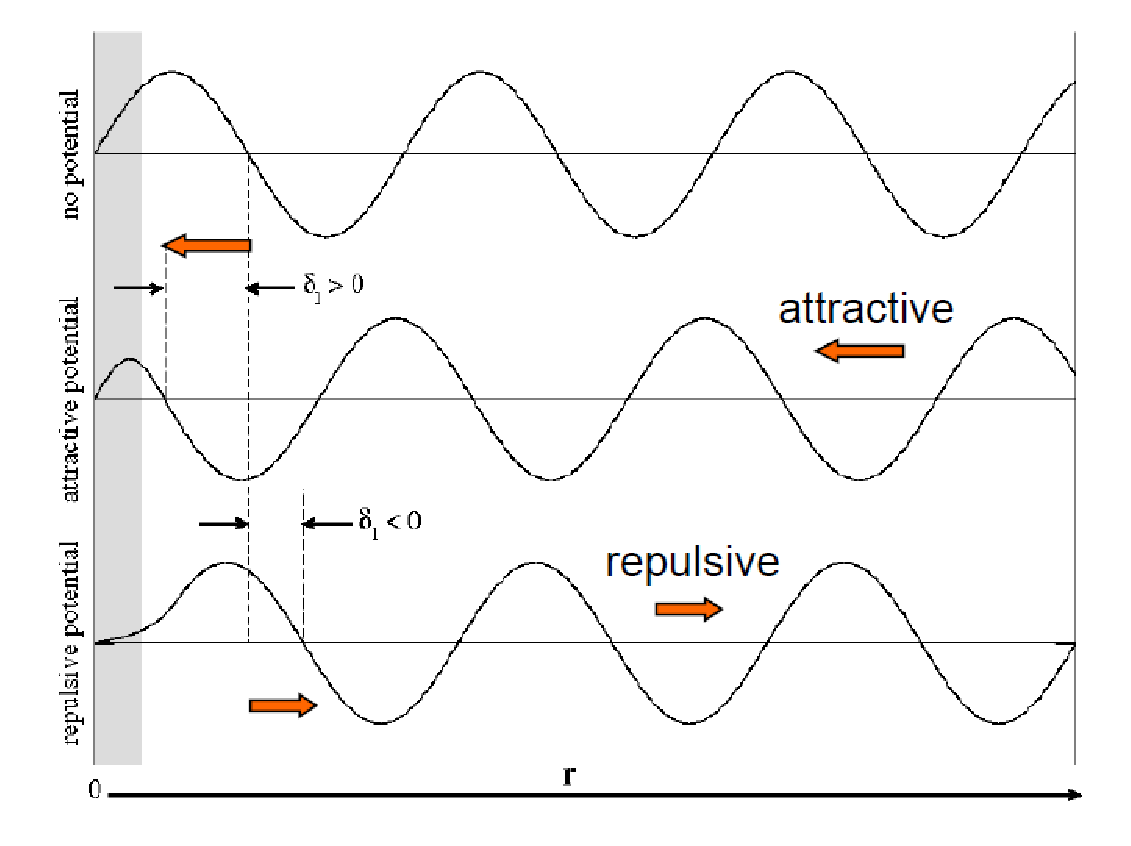
\includegraphics{\images/phaseshifts.eps}} \par}
%\end{figure}
%}%only




\end{frame}




% -------------------------------------------------------------------------
\slide{The scattering amplitude}

\begin{itemize}
\gitem {Replace the asymptotic $\chi_{\ell}(K,R)$ in the general expansion:}

\begin{center}
\psframebox[fillcolor=magenta!5,linecolor=red,framearc=0.1,fillstyle=solid,framesep=-7pt]{
\parbox{0.8\textwidth}{
\begin{align*}
\chi^{(+)}_0 (\bK,\bR) &  \rightarrow  \frac{1}{K R} \sum_{\ell} i^\ell (2 \ell +1)
   {\blue \left \{  F_\ell(K R) +  T_\ell H^{(+)}_\ell (K R)  \right \} }
    P_{\ell}(\cos \theta)   \\
%                         & =  \frac{1}{K R} \sum_{\ell} i^\ell  (2 \ell +1) F_\ell(K R) P_{\ell}(\cos \theta) + 
% \frac{1}{K} \sum_{\ell } i^\ell (2 \ell +1)   T_\ell    \frac{e^{i (K R-\ell \pi/2)}}{R}   P_{\ell}(\cos \theta)  \\
                         & =  e^{i \bK \cdot \bR}  + 
 \frac{1}{K} \sum_{\ell }   (2 \ell +1)  e^{i \delta_\ell} \sin{\delta_\ell}     P_{\ell}(\cos \theta) \frac{e^{i K R}}{R} 
\end{align*}
}%parbox
}%psframe
\end{center}

\gitem{The scattering amplitude is the coefficient of  $e^{i K R}/{R}$:}
\begin{center}
\psframebox[fillcolor=magenta!5,linecolor=red,framearc=0.1,fillstyle=solid,framesep=-7pt]{
\parbox{0.7\textwidth}{
\begin{align*} 
f(\theta)  & = \frac{1}{K} \sum_{\ell} (2 \ell +1)  e^{i \delta_\ell} \sin{\delta_\ell}  P_{\ell}(\cos \theta) 
 \\
          & = \frac{1}{2 i K} \sum_{\ell}(2 \ell +1) (S_\ell -1 ) P_{\ell}(\cos \theta) .
\end{align*} 
}%parbox
}%psframe
\end{center}

\gitem{Elastic cross section:}
$$
\frac{d\sigma}{d\Omega} = | f(\theta) | ^ 2  .
$$ 
\end{itemize}

\end{frame}



% -------------------------------------------------------------------------
\slide{Coulomb plus nuclear case}
{\verde Radial equation:}
\begin{columns}
%\column{0.5\linewidth}
\begin{column}[t]{0.55\textwidth}
$$
\psframebox[fillcolor=magenta!5,linecolor=red,framearc=0.1,framesep=2pt]{
\left [ \frac{d^2}{dR^2} + K^2 - {\blue \frac{2 \eta K}{R}} +
   \frac{2 \mu}{\hbar^2}U(R)+ \frac{\ell (\ell +1)}{R^2} \right ]  \chi_\ell(K, R) = 0
}%psframe
$$
\end{column} %\hfill
\hspace{0.5cm}
\begin{column}[t]{0.4\textwidth}
\vspace{0.4cm}
%\hspace{1.5cm}
%\hfill
$$
\small
\psframebox[linecolor=blue,framearc=0.1,framesep=2pt]{
\eta= \frac{Z_p Z_t e^2}{\hbar v } = \frac{Z_p Z_t e^2 \mu}{\hbar^2 K}
}%psframe
$$
\begin{center}(Sommerfeld parameter) \end{center}
\end{column}
\end{columns}



%\begin{block}{Pure Coulomb wave}
%\end{block}

{\verde Asymptotic condition:}
$$
\chi^{(+)}(\bK,\bR)  \rightarrow e^{i [\bK \cdot \bR +\eta \log (kR-\bK \cdot \bR )]}+ 
                    f(\theta) \frac{e^{i ( KR- \eta \log 2 K R)}}{R}  
$$

%\begin{block}{Asymptotic condition}

\begin{columns}
\column{0.55\columnwidth}
\small
\psframebox[fillcolor=magenta!5,linecolor=red,framearc=0.1,fillstyle=solid,framesep=0pt]{
\parbox{0.95\textwidth}{
\begin{align*}
\chi_\ell (K,R) & \rightarrow {\red e^{i \sigma_\ell}} \left [ F_\ell (\eta,KR) + T_\ell H^{(+)}_\ell (\eta, KR)  \right ]  \\
              & = (i/2) {\red e^{i \sigma_\ell}}\left [  H^{(-)}_\ell  (\eta,KR) -S_\ell H^{(+)}_\ell (\eta, KR)  \right ] 
\end{align*}
}%parbox
}%psframe
\column{0.44\columnwidth}
\small
\ding{43} $\sigma_{\ell} (\eta)$=Coulomb phase shift \\
\ding{43} $F_{\ell} (\eta,KR)$=regular Coulomb wave \\
\ding{43} $H^{(\pm)}_\ell (\eta,KR)$=outgoing/ingoing Coulomb wave
%\end{block}
\end{columns}
\end{frame}








% -------------------------------------------------------------------------
\slide{Coulomb plus nuclear case: scattering amplitude}

Total scattering amplitude:
$$
\psframebox[fillcolor=magenta!5,linecolor=red,framearc=0.1,fillstyle=solid,framesep=7pt]{
f(\theta) = f_C (\theta) + \frac{1}{2 i K} \sum_{\ell} (2 \ell +1) e^{2 i \sigma_\ell} (S_\ell -1) P_\ell(\cos \theta)
}%psframe
$$

\ding{43}
$f_C(\theta)$ is the amplitude for pure Coulomb:

$$
\psframebox[fillcolor=magenta!5,linecolor=red,framearc=0.1,fillstyle=solid,framesep=7pt]{
\frac{d\sigma_R}{d \Omega} = |f_C(\theta)|^2 = \frac{\eta^2}{4 K^2 \sin^4(\frac{1}{2}\theta) } = 
\left ( \frac{Z_p Z_t e^2}{4 E}  \right )^2  \frac{1}{\sin^4(\frac{1}{2}\theta)}
}%psframe
$$

\end{frame}

%-----------------------------------
\slide{Integrated cross sections}

\begin{itemize}
\item Total {\blue elastic} cross section (uncharged particles!)
$$
\psframebox[fillcolor=magenta!5,linecolor=red,framearc=0.1,fillstyle=none,framesep=2pt]{
\sigma_{el} = \int d\Omega \frac{d\sigma}{d\Omega} = \frac{\pi}{K^2} \sum_{\ell} (2 \ell + 1) |1 - S_\ell|^2  
}%
$$
 
\item Total {\blue reaction} cross section (loss of flux from elastic channel) 
$$
\psframebox[fillcolor=magenta!5,linecolor=red,framearc=0.1,fillstyle=none,framesep=2pt]{
\sigma_{reac} = \frac{\pi}{K^2} \sum_{\ell} (2 \ell + 1) (1 - |S_\ell|^2) =\frac{\pi}{K^2} \sum_{\ell} (2 \ell + 1) |T_\ell|^2  
}%
$$


\end{itemize}

\end{frame}







% ----------------------------------------------------------------------------------
\slide{$^4$He+$^{58}$Ni example}


{\brick Effective potential:} $U(R)= U_{nuc}(R) +  U_{coul}(R) $

\begin{figure}{\par \resizebox*{0.5\textwidth}{!}
{\includegraphics{\images/he4ni_veff.eps}} \par}
\end{figure}
\ding{43} The maximum of $V_\mathrm{nuc}(R)+V_C(R)$ defines the Coulomb barrier. Approximately:
$$
\psframebox[fillcolor=magenta!5,linecolor=red,framearc=0.1,fillstyle=none,framesep=2pt]{
R_b \simeq 1.44(A_p^{1/3} + A_t^{1/3})~\textrm{fm}
}%psframe
\quad
\psframebox[fillcolor=magenta!5,linecolor=red,framearc=0.1,fillstyle=none,framesep=2pt]{
 E_b \simeq \frac{Z_p Z_t e^2}{R_b}=\frac{Z_p Z_t}{(A_p^{1/3} + A_t^{1/3})} ~ \textrm{MeV}
}%psframe
$$
\end{frame}
% ----------------------------------------------------------------------------------




% -------------------------------------------------------------------------
\slide{Effect of indicent energy}
%------------------------------------------------------------------------

\ding{43} Depending on the bombarding energy $E$ and the charges of the interacting nuclei, we observe different patterns 
 of elastic scattering. 

\vspace{0.5cm}
\ding{43} For medium/heavy systems, this can be characterized in terms of the Coulomb (or Sommerfeld) parameter: 
{\blue $$\eta = {Z_p Z_t  e^2 \over  4 \pi \epsilon_0 \hbar v}$$ }

%\vspace{0.5cm}
\begin{itemize}
\setlength{\itemsep}{16pt}
\gitem{$E$ well above the Coulomb barrier} {\blue ($\eta \lesssim 1$)} $\Rightarrow$ Fraunhofer scattering
\gitem{$E$ around the Coulomb barrier} {\blue ($\eta \gg 1$)} $\Rightarrow$ Fresnel scattering
\gitem{$E$ well below the Coulomb barrier} {\blue ($\eta \ggg 1$)} $\Rightarrow$ Rutherford scattering 
\end{itemize}

\end{frame}



% ----------------------------------------------------------------------------------
\slide{Elastic scattering: energy dependence}


% --------------- Absolute cross sections --------
\begin{minipage}[t]{.32\textwidth}
\begin{figure}{\par \resizebox*{0.75\textwidth}{!}
{\includegraphics{\images/he4ni_e5_abs.eps}} \par}
\end{figure}
%\center{Rutherford  scattering}
\end{minipage}
% -----------------------------------------------
\begin{minipage}[t]{.32\textwidth}
\begin{figure}{\par \resizebox*{0.75\textwidth}{!}
{\includegraphics{\images/he4ni_e10_abs.eps}} \par}
\end{figure}
%\center{Fresnel}
\end{minipage}
% -----------------------------------------------
\begin{minipage}[t]{.32\textwidth}
\begin{figure}{\par \resizebox*{0.75\textwidth}{!}
{\includegraphics{\images/he4ni_e25_abs.eps}} \par}
\end{figure}
%\center{Fraunh\"ofer}
\end{minipage}
% -----------------------------------------------

\vspace{0.5cm}

% --------------- Relative cross sections ---------------------
\begin{minipage}[t]{.32\textwidth}
\begin{figure}{\par \resizebox*{0.75\textwidth}{!}
{\includegraphics{\images/he4ni_e5.eps}} \par}
\end{figure}
\center{\bf Rutherford  scattering }
\end{minipage}
% -----------------------------------------------
\begin{minipage}[t]{.32\textwidth}
\begin{figure}{\par \resizebox*{0.75\textwidth}{!}
{\includegraphics{\images/he4ni_e10.eps}} \par}
\end{figure}
\center{\bf Fresnel}
\end{minipage}
% -----------------------------------------------
\begin{minipage}[t]{.32\textwidth}
\begin{figure}{\par \resizebox*{0.75\textwidth}{!}
{\includegraphics{\images/he4ni_e25.eps}} \par}
\end{figure}
\center{\bf Fraunh\"ofer}
\end{minipage}
% -----------------------------------------------

\end{frame}
% --------------------------------------------------------------------------------------




% ----------------------------------------------------------------------------------
\slide{Effect of indicent energy (cont.)}

{\bf \brick Example:}  {\bf \nuc{4}{He}+\nuc{58}{Ni} at E=5, 10.7, 25 and 50 MeV} 

\medskip

\ding{43} {\bf Coulomb barrier:} $R_b\simeq 7.8$~fm ; ~~~ $V_b\simeq 10.2$~MeV


\medskip

{\large 
\begin{center}

 \begin{tabular}{|ccccc|}
\hline
 {\blue \bf $E_\mathrm{lab}$ } &  {\blue \bf $\eta$} &  {\blue \bf $ K$ } &  {\blue \bf  $\lambdabar=1/K$}  & {\blue \bf $2 a_0$(*)} \\
(MeV)    &                    &       (fm$^{-1}$)      &  (fm)            & (fm)         \\   
\hline
  5      &      7.95       &         0.920        & 1.087     &      17.2  \\
10.7     &      5.62       &         1.34         & 0.746     &      8.06  \\
25       &      3.55       &         2.06         & 0.485     &      3.44   \\
50       &      2.51       &         2.91         & 0.343     &      1.69  \\
\hline
 \end{tabular}
\end{center}
{\small (*) classical distance of closest approach in head-on collision.}

\bigskip

%\ding{43} ${\blue \eta = {Z_1 Z_2  e^2 \over  4 \pi \epsilon_0 \hbar v} }$

\begin{itemize}
\item {\bf \blue $\eta \ggg 1$}: Rutherford scattering: 
{\verde $\sigma (\theta) \propto 1/\sin^4(\theta/2)$}
\item {\bf \blue $\eta \gg  1$}: Fresnel scattering (rainbow)
\item {\bf \blue $\eta \leq 1$}: Fraunhofer scattering (oscillatory behaviour): 
\end{itemize}


}%large
\end{frame}




% -------------------------------------------------------------------------
\slide{Rutherford scattering}

%{\sc \brick Rutherford scattering}


\begin{columns}
\column{0.5\textwidth}
\begin{figure}{\par \resizebox*{0.8\textwidth}{!}
{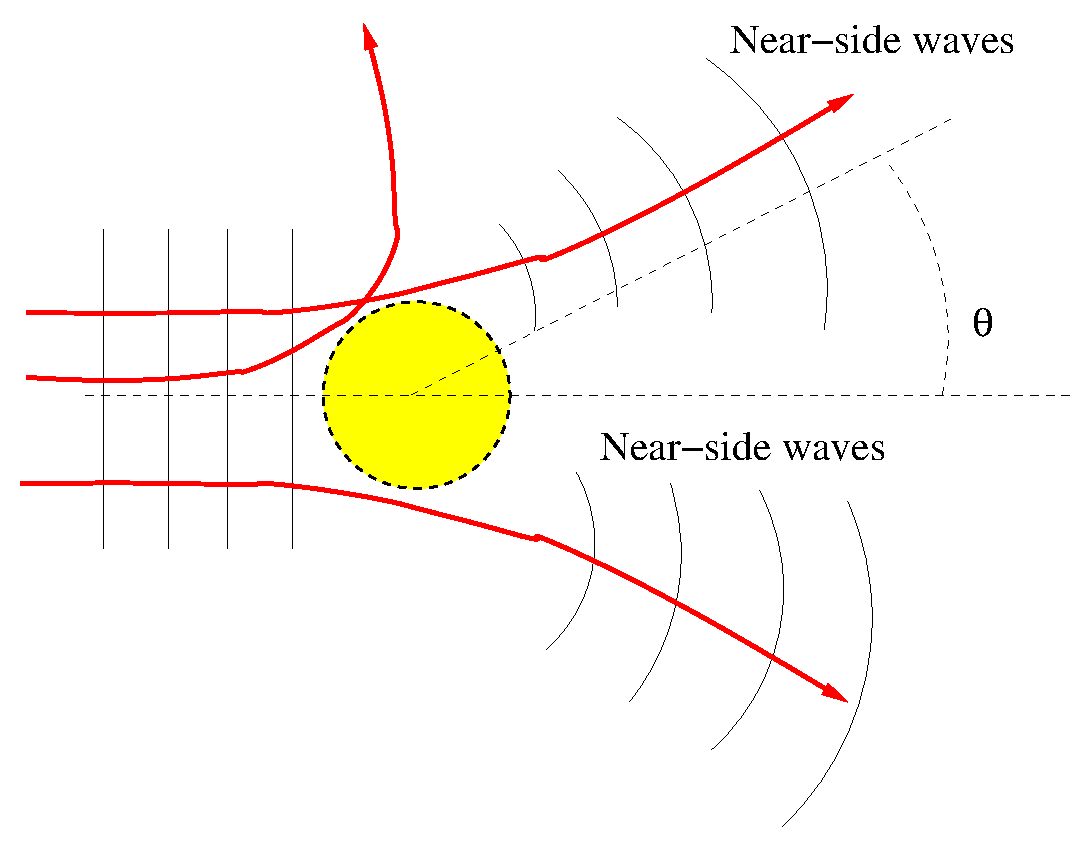
\includegraphics{\images/rutherford.eps}} \par}
\end{figure}
\column{0.5\textwidth}
\begin{figure}{\par \resizebox*{0.65\textwidth}{!}
{\includegraphics{\images/he4ni_e5_abs.eps}} \par}
\end{figure}
\end{columns}


\begin{itemize}
 \item Bombarding energy well below the Coulomb barrier
 \item Purely Coulomb potential ({\verde $\eta \ggg 1$})
 \item Obeys Rutherford law:   
   {\blue $${d \sigma \over d \Omega} = {Z_p Z_t  e^2 \over 4 E} {1 \over \sin^4 (\theta/2)}$$.}
\end{itemize} 

\end{frame}



% -------------------------------------------------------------------------
\slide{Fraunhofer scattering}

%{\sc \brick FRAUNHOFER scattering:}
%\vspace{0.25cm}

\begin{columns}
\column{0.5\textwidth}
\begin{figure}{\par \resizebox*{1.0\textwidth}{!}
{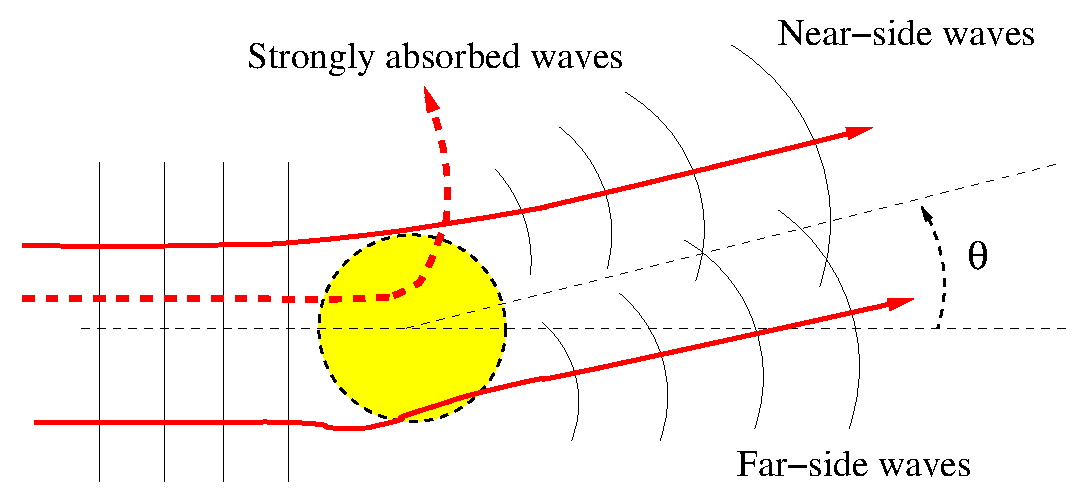
\includegraphics{\images/fraunhofer.eps}} \par}
\end{figure}
\column{0.5\textwidth}
\only<1>{
\begin{figure}{\par \resizebox*{0.65\textwidth}{!}
{\includegraphics{\images/he4ni_e25.eps}} \par}
\end{figure}
}%only
\only<2>{
\begin{figure}{\par \resizebox*{0.65\textwidth}{!}
{\includegraphics{\images/he4ni_e25_nearfa.eps}} \par}
\end{figure}
}%only

\end{columns}

\bigskip

\begin{itemize}
\item Bombarding energy well above Coulomb barrier
\item Coulomb weak ({\verde $\eta \lesssim 1$})
\item Nearside/farside interference pattern  (difracction) 
\end{itemize}

\end{frame}



% -------------------------------------------------------------------------
\slide{Fresnel scattering}

%{\sc \brick FRESNEL scattering:}

%\vspace{0.25cm}


\begin{columns}
\column{0.5\textwidth}
\begin{figure}{\par \resizebox*{0.8\textwidth}{!}
{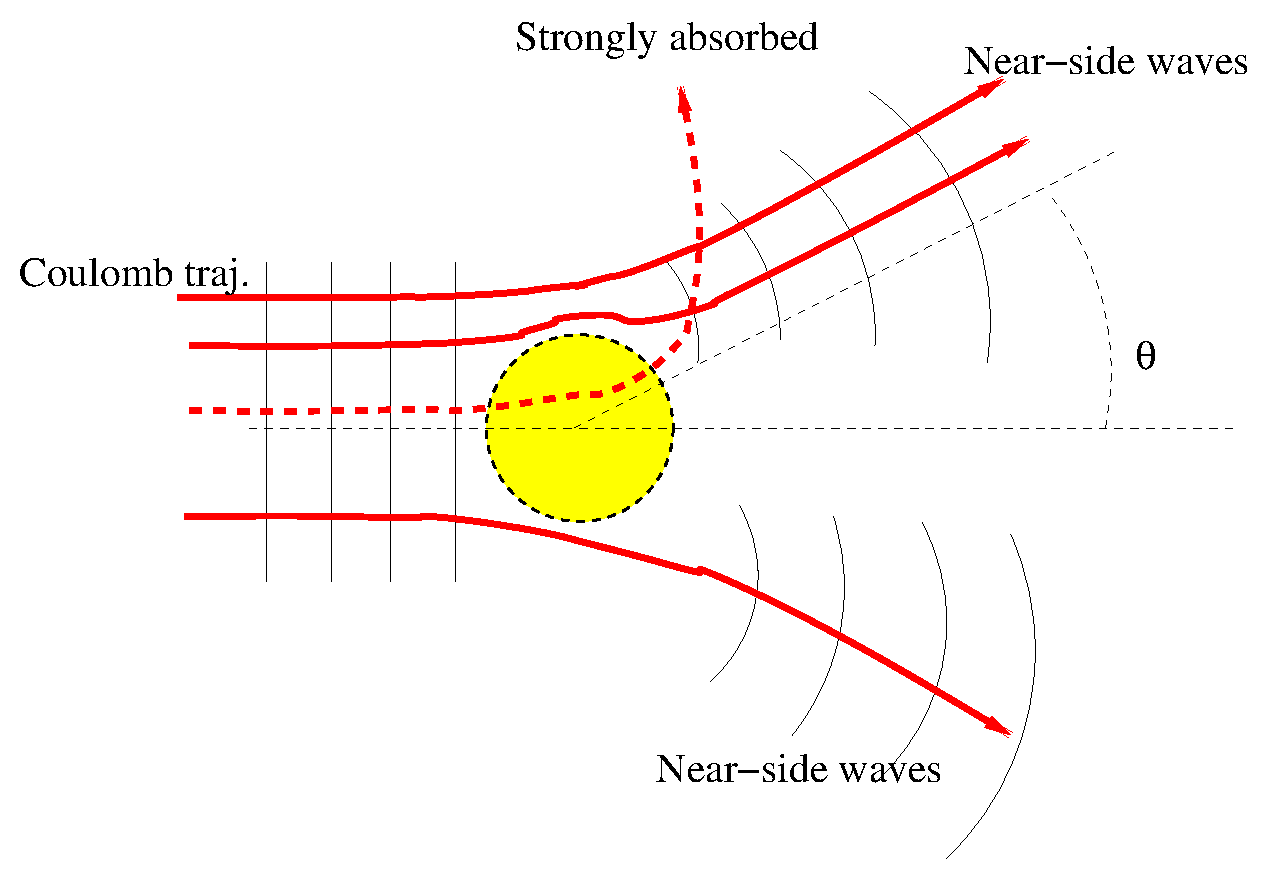
\includegraphics{\images/fresnel.eps}} \par}
\end{figure}
\column{0.5\textwidth}
\begin{figure}{\par \resizebox*{0.65\textwidth}{!}
{\includegraphics{\images/he4ni_e10.eps}} \par}
\end{figure}
\end{columns}


\bigskip

\begin{itemize}
\item Bombarding energy around or near the Coulomb barrier
\item Coulomb strong ({\verde $\eta \gg 1$})
\item  'Illuminated' region $\Rightarrow$ Coulomb + nuclear trajectories
\item[] 'Shadow' region $\Rightarrow$ strong absorption
\end{itemize}

\end{frame}





\subsection{Elastic scattering of weakly-bound nuclei}
% ---------------------------------------------------------------------------------------------------
\slide{Normal versus halo nuclei}

{\verde How does the halo structure affect the elastic scatterig?}
\vspace{0.3cm}


\begin{columns}
\column{0.5\textwidth}
\begin{figure}{\par \resizebox*{0.7\textwidth}{!}
{\includegraphics{\images/he4pb_e22.eps}} \par}
\end{figure}
\column{0.5\textwidth}
\begin{figure}{\par \resizebox*{0.7\textwidth}{!}
{\includegraphics{\images/he6pb_e22.eps}} \par}
\end{figure}
\end{columns}
\bigskip

\begin{small}
\begin{itemize}
\item \nuc{4}{He}+\nuc{208}{Pb} shows typical Fresnel pattern and ``standard'' optical model parameters
%$\rightarrow$ {\blue \em strong absorption} 
\item \nuc{6}{He}+\nuc{208}{Pb} shows a prominent reduction in the elastic cross section, suggesting that part of the incident flux goes to non-elastic channels (eg.~breakup) 
\item[] Understanding and disentangling these non-elastic channels requires going beyond the optical model (eg.~{\blue coupled-channels method} $\Rightarrow$ next lectures) 
\end{itemize}
\end{small}
%}%onslide
\end{frame}


% ------------------------------------------------------------------------------------------------
\slide{Origin of the long-range absorption in $^6$He}

\small
\begin{columns}
\column{0.5\textwidth}

\begin{center}\includegraphics[height=4.5cm]{\images/6he-tidal.eps} \end{center}

\column{0.5\textwidth}
\begin{center}\includegraphics[height=4.5cm]{\images/be1-he6.eps} \end{center}
\end{columns}

\bi
\item[\ding{233}] The Coulomb force on the core induces a tidal force which may eventually break $^{6}$He.
\item[\ding{233}] From the structure point of view, this translates into a large $B(E1)$ strength near breakup threshold.
\ei
\end{frame}




%----------------------------------------------------------
\slide{Second order perturbative amplitude}

\begin{center}
\psframebox[fillcolor=magenta!5,linecolor=red,framearc=0.1,fillstyle=solid,framesep=-8pt]{
\parbox{0.75\textwidth}{
\begin{align*}
c^{(2)}_n = & \sum_{z} \left({-i \over \hbar}\right)^2 
  \int_{-\infty}^{+\infty} dt {\red \langle  n | V_1(t) | z \rangle}
  \exp \left\{ {i \over \hbar}(E_n - E_z) t \right\} \\
 & \times 
  \int_{-\infty}^{t} dt' {\red \langle  z | V_1(t') | 0 \rangle}
  \exp \left\{ {i \over \hbar}(E_z - E_0) t' \right\}
\end{align*}
}%parbox
}%psframe
\end{center}

\begin{center}\includegraphics[width=0.8\columnwidth]{\images/a1_traj.eps}  \end{center}

\end{frame}


% --------------------------------------------------------------------------------------
\slide{\small How does a weakly bound nucleus behaves in the field of a heavy target?}

\begin{enumerate}
\item The strong Coulomb field will produce a polarization (``stretching'') of the projectile, giving rise 
to a dipole contribution on the \textcolor{blue}{real} potential:
$$V(R) \approx \frac{Z_1 Z_2 e^2}{R} - \alpha \frac{Z_1 Z_2 e^2}{2 R^4}$$

\item The weakly bound nucleus can eventually break up, leading to a loss of flux of the elastic channel $\Rightarrow$ \textcolor{blue}{imaginary} polarization potential.
\end{enumerate}

\end{frame}



% ---------------------------------------------------------------------------------------------------
\slide{The effect of E1 on elastic scattering of weakly-bound nuclei}

\begin{columns}
\column{0.5\textwidth}
\begin{figure}{\par \resizebox*{0.86\textwidth}{!}
{\includegraphics{\images/he6pb_e22_om.eps}} \par}
\end{figure}
\column{0.5\textwidth}
\begin{figure}{\par \resizebox*{0.7\textwidth}{!}
{\includegraphics{\images/he6pb_cdp.eps}} \par}
\end{figure}
\end{columns}
\bigskip

\begin{small}
\begin{itemize}
\item E1 Coulomb couplings produces a sizable effect on the elastic cross section of neutron-halo nuclei (we have learnt something!) but...some additional physics is still missing. 
\end{itemize}
\end{small}
%}%onslide
\end{frame}




%---------------------------------------------------------------------------------------
\slide{Eg: deuteron polarizability from d+\nuc{208}{Pb}: }

\begin{itemize}
\setlength{\itemsep}{0pt}
%\item[\ding{43}] Deuteron polarizability: $\mathbf{P}= \alpha \mathbf{E}$ 
%\item[\ding{43}] For $E< V_b$,  the main deviation from Rutherford scattering comes from dipole polarizability. 
\item[\ding{43}] Adiabatic limit ($E_x \gg$ ): $V_\mathrm{pol}^\mathrm{dip}=- \alpha \frac{Z_1 Z_2 e^2}{2 R^4}$
\end{itemize}

%\psshadowbox[fillcolor=lightgreen]{{\sc \brick Radius of sensitivity of V(r) and W(r)}}

\begin{columns}[c]
\column{.5\textwidth}
\begin{figure}{\par \resizebox*{0.75\textwidth}{!}
{\includegraphics{\images/RE.eps}} \par}
\end{figure}
\column{.5\textwidth}
\begin{figure}{\par \resizebox*{0.75\textwidth}{!}
{\includegraphics{\images/dpb_scattering.eps}} \par}
\end{figure}
\end{columns}%twocolumn
\medskip
\small 
\textcolor{verde}{\small Rodning et al, PRL49, 909 (1982)} $\Rightarrow$ \textcolor{red}{$\alpha = 0.70 \pm 0.05 $~fm$^3$}

\end{frame}

\endinput

%%%%%%%%%%%%%%%%%%%%%%
% BACKUP SLIDES FOR ELASTICS
%%%%%%%%%%%%%%%%%%%%%%
\slide{}
\begin{center}
\psframebox[fillcolor=green!10,linecolor=blue,framearc=0.1,fillstyle=solid,framesep=5pt]{
SUPPLEMENTARY MATERIAL
}%psframe
\end{center} 
\end{frame}





% ---------------------------------------------------------------------------
\slide{Grazing radius and angular momentum}

\begin{itemize}
\setlength{\itemsep}{14pt}
\item Grazing collisions are those for which $b \approx R_1 + R_2 = R_g$ 

\item Relation with angular momentum:
\begin{enumerate}
\item {\blue Only nuclear:} $b K = \sqrt{\ell (\ell +1) } \simeq \ell +1/2$
$$
\psframebox[fillcolor=magenta!5,fillstyle=solid,linecolor=red,framearc=0.1]{
K R_g \simeq \ell_g +1/2
}
 \quad (\ell_g=\textrm{grazing angular momentum})
$$
\item {\blue Nuclear + Coulomb:}
$$
\psframebox[fillcolor=magenta!5,fillstyle=solid,linecolor=red,framearc=0.1]{
K R_g \left(1- 2 \eta /K R_g  \right)\approx \ell_g +1/2 
}%
$$
\end{enumerate}

\item[\ding{233}] As $E$ increases, so does the number of partial waves involved
\item[\ding{233}] Peripherical processes (inelastic, transfer) occur mainly around $\ell \sim \ell_g$
\end{itemize}

\end{frame}




% ----------------------------------------------------------------------------------
\slide{Elastic scattering: S-matrix elements}

{\brick Elastic (nuclear) S-matrix :} $\chi_{\ell}(K,R) =H^{(-)}_{\ell}(R) -  S_\ell H^{(+)}_\ell(R)$


\vspace{0.5cm}

\begin{columns}
\column{0.5\textwidth}
\begin{figure}{\par \resizebox*{0.95\textwidth}{!}
{\includegraphics{\images/4he58ni_smat.eps}} \par}
\end{figure}
\column{0.5\textwidth}
\begin{figure}{\par \resizebox*{0.95\textwidth}{!}
{\includegraphics{\images/4he58ni_reac.eps}} \par}
\end{figure}
\end{columns}

\medskip

\begin{center}
{\blue  $K R_g \left(1- 2 \eta /K R_g  \right)\approx \ell_g +1/2$} 
\end{center}


$\Rightarrow$ the number of partial waves 
required for convergence grows approximately as $\sqrt{E}$ 


\end{frame}

\endinput

% --------------------------------------------------------------------------
\slide{Elastic scattering phenomenology }


{\bf \verde What can we learn from the  analysis of the elastic cross section?}

\vspace{1cm}

% --------------- Absolute cross sections --------
\begin{minipage}[t]{.32\textwidth}
\begin{figure}{\par \resizebox*{0.84\textwidth}{!}
{\includegraphics{\images/dni_e80_el_dat.eps}} \par}
\end{figure}
%\center{Rutherford  scattering}
\end{minipage}
% -----------------------------------------------
\begin{minipage}[t]{.32\textwidth}
\begin{figure}{\par \resizebox*{0.84\textwidth}{!}
{\includegraphics{\images/he4pb_e22_exp.eps}} \par}
\end{figure}
%\center{Fresnel}
\end{minipage}
% -----------------------------------------------
\begin{minipage}[t]{.32\textwidth}
\begin{figure}{\par \resizebox*{0.84\textwidth}{!}
{\includegraphics{\images/he6pb_e22_data.eps}} \par}
\end{figure}
%\center{Fraunh\"ofer}
\end{minipage}
% -----------------------------------------------

\bigskip

\end{frame}







\section{Inelastic scattering}

\subsection{General features of inelastic scattering}

\slide{}
\begin{center}
\psframebox[fillcolor=green!10,linecolor=blue,framearc=0.1,fillstyle=solid,framesep=5pt]{
Inelastic scattering
}%psframe
\end{center} 
\end{frame}

% --------------------------------------------------------------------------------------
\slide{Inelastic scattering}
\begin{itemize}
\item Nuclei are not inert or {\em frozen} objects; they do have an internal structure of protons and neutrons
that can be modified (excited) during the collision.
\item Quantum systems exhibit, in general, an energy spectrum with bound and unbound levels.
\end{itemize}

\begin{columns}
\column{0.5\textwidth}
\begin{figure}{\par \resizebox*{0.75\textwidth}{!}
{\includegraphics[angle=0]{\images/be11pb_inel.eps}} \par}
\end{figure}
\column{0.5\textwidth}
\begin{figure}{\par \resizebox*{0.5\textwidth}{!}
{\includegraphics[angle=0]{\images/be11_spectrum_crop.eps}} \par}
\end{figure}
\end{columns}
\end{frame}


%----------------------------------------------------------------------------------------
\slide{Models for inelastic excitations}

\begin{enumerate}
\ritem{\sc COLLECTIVE:} Involve a collective motion of several nucleons which can be interpreted macroscopically as {\verde rotations} or  {\verde surface vibrations} of the nucleus.
 \begin{figure}{\par \resizebox*{0.15\textwidth}{!}
{\includegraphics{\images/deformed-nucleus.eps}} \par}
\end{figure}

\ritem{\sc FEW-BODY/SIGLE-PARTICLE:} Involve the excitation of a nucleon or cluster.
\begin{figure}{\par \resizebox*{0.3\textwidth}{!}
{\includegraphics[angle=0]{\images/be11pb_inel.eps}} \par}
\end{figure}
\end{enumerate}

\end{frame}


% ----------------------------------------------------------------------------------
\slide{Types of collective excitations}

\only<1>{
The nucleons can move inside the nucleus in a coherent (collective) way.

\begin{enumerate}
\gitem{Vibrations} (spherical nuclei): small surface oscillations in shape.
\begin{figure}{\par \resizebox*{0.25\textwidth}{!}
{\includegraphics{\images/vibrations.eps}} \par}
\end{figure}
\gitem{Rotations} (non-spherical nuclei): permanent deformation.
\gitem{Monopole} ({\em breathing}) mode: oscillations in the size (radius). 
\gitem{Isovector} excitations (protons and neutrons move out of phase) (eg. giant dipole resonance)
\end{enumerate}
}
\only<2>{
\ding{43} The type of collective motion is closely related to the kind of energy spectrum.
\begin{itemize} 
\item Rotor: $E_J \propto J(J+1)$
\item Vibrator: $E_J \approx n \hbar \omega$
\end{itemize}

\begin{figure}{\par \resizebox*{0.7\textwidth}{!}
%{\includegraphics{\images/vibrational-rotational-spectrum.eps}} \par}
{\includegraphics{\images/samarium.eps}} \par}
\end{figure}
}%onslide
\end{frame}



%------------------------------------------------------------
\slide{Microscopic description in the IPM: the $^{11}$Be case} 

\begin{center}\includegraphics[angle=0,height=0.33\textheight]{\images/be11_spectrum_crop.eps} \end{center}

\bc
\column{0.5\linewidth}
\begin{center}  \psframebox[fillcolor=green!15,linecolor=blue,framearc=0.1,fillstyle=solid]{Ground state ($1/2^+$)} \end{center}
\begin{center} \includegraphics[width=0.45\columnwidth]{\images/be11_capas_inert.eps} \end{center}

\column{0.5\linewidth}
\begin{center} \psframebox[fillcolor=green!15,linecolor=blue,framearc=0.1,fillstyle=solid]{First excited state ($1/2^-$)}  \end{center}
\begin{center} \includegraphics[width=0.45\columnwidth]{\images/be11_capas_j12n.eps} \end{center}
\ec

\end{frame}

%----------------------------------------------------------------------------------------
\slide{Models for inelastic excitations}
{\blue Microscopically}, what we describe in both cases are quantum transitions between discrete or continuum states:

%\vspace{1cm}

\begin{columns}
\column{0.5\textwidth}
\begin{figure}{\par \resizebox*{0.65\textwidth}{!}
{\includegraphics[angle=0]{\images/o16_spectrum.eps}} \par}
\end{figure}
\column{0.5\textwidth}
\begin{figure}{\par \resizebox*{0.5\textwidth}{!}
{\includegraphics[angle=0]{\images/be11_spectrum_crop.eps}} \par}
\end{figure}
\end{columns}

\vspace{0.5cm}

\ding{43}{\em \magenta Collective excitations can be regarded as a coherent superposition of many single-particle excitations.}
\end{frame}


%-------------------------------------------------------------------------------------------------------
\slide{}
\begin{itemize}
\item By doing inelastic scattering experiments we {\it measure} the {\it response} of the nucleus to an external field (Coulomb, nuclear). This response is related to some structure property of the nucleus. 

\item[] Example: for a {\brick Coulomb} field:

$$ % BM convention 
\psframebox[linecolor=red,framearc=0.1]{
B(E\lambda; i \to f) = \frac{1}{2I_i +1} |\langle \Psi_f | {\cal M}(E \lambda) | \Psi_i \rangle |^2 
}
$$ 
where {\brick ${\cal M}(E\lambda, \mu)$}  is the electric multipole operator:
$$
\psframebox[linecolor=red,framearc=0.1]{
 {\cal M}(E\lambda, \mu) \equiv e \sum_i^{Z_p} r_i^\lambda  Y_{\lambda \mu}^{*}(\hat r_i) 
}%ps
$$


\item The structure $\Psi_{i,f}$ can be described in a collective, few-body or microscopic model. 

% \begin{center}
% $$ 
% \psframebox[fillcolor=green!15,linecolor=blue,framearc=0.1,fillstyle=solid]
%   {\mathrm{Probability} \propto |\langle \Psi(2^+) | \hat{V} | \Psi(gs;0^+) \rangle|^2 }   
% $$ 
% \end{center}

%This process can be treated in different ways:
%\begin{itemize}
%\item {\bf Microscopic}: treat all nucleons of the nucleus being excited 
%\item {\bf Collective}: defining some collective (macroscopic) parameters measuring the strength of these couplings. 
%\item {\bf Few-body}: Grouping some nucleons in clusters corresponding to more compact structures. 
%\end{itemize}

\end{itemize}

\end{frame}


% ----------------------------------------------------------------------------------------------------
\slide{Multi-channel case: the coupled-channels method}
We need to incorporate explicitly in the Hamiltonian the internal structure of the nucleus being excited (eg.~ {\verde target}).
$$ 
\psframebox[linecolor=red,framearc=0.1]{
 H = T_R   +  h(\xi)+ V(\bR, \xi)
}
$$


\begin{itemize}
\gitem{$T_R$}: Kinetic energy for projectile-target relative motion.
\gitem{$\{\xi\}$}: Internal degrees of freedom of the target (depend on the model).
\gitem{$h(\xi)$}: Internal Hamiltonian of the target.
$$
\psframebox[linecolor=red,framearc=0.1]{
h(\xi)\phi_{n}(\xi)  =  \varepsilon_{n}\phi_{n}(\xi)
}
$$

\gitem{$V(\bR, \xi)$}: Projectile-target interaction.
%, eg:
%$$
%V(\bR, \xi) = \sum_{i=1}^{N} V_{pi}(\br_{pi})
%$$

% \pause 
% \item[] {\bf Eg.:} $^7$Li=$\alpha+t$ $\Rightarrow$ {\verde $\{\xi\} \equiv \bf r$}
% $$
% V_\mathrm{p-7Li}({\bf R}, {\bf r})= V_\mathrm{p-t}\left({\bf R} +\frac{4}{7}{\bf r}\right) 
% + 
% V_\mathrm{p-\alpha}\left({\bf R} +\frac{3}{7}{\bf r}\right)
% $$
\end{itemize}
\end{frame}




% ----------------------------------------------------------------------------------------------------
\slide{Defining the modelspace: d+\nuc{10}{Be} $\rightarrow$ d+\nuc{10}{Be*} example}

\begin{center}
\begin{columns}
\column{0.6\textwidth}
\hspace{2cm}\includegraphics[width=0.4\columnwidth]{\images/be10d_modelspace_ine.eps}
\column{0.4\textwidth}
\psframebox[fillcolor=yellow!25,linecolor=black,fillstyle=solid,framearc=0.1]{
\parbox{0.8\columnwidth}{
 \ding{43} P space composed by ground states (elastic channel) and some excited states (inelastic scattering)  
}%parbox
}%frame
\end{columns}
\end{center}

Boundary conditions:

$$
 \Psi^{(+)}_{\bK_0}(\bR,\xi)   \xrightarrow{R \gg}  \underbrace{\vphantom{\sum_{n>0}} e^{i \bK_0 \cdot \bR} \phi_0(\xi)}_{\mathrm{\blue incident}}   
                          +  \underbrace{\vphantom{\sum_{n>0}} {\red f_{0,0}(\theta)} \frac{e^{i K_0 R}}{R} \phi_0(\xi)}_{\mathrm{\blue elastic}}
                          + \underbrace{\sum_{n>0} {\red f_{n,0}(\theta)}  \frac{e^{i K_n R}}{R}  \phi_n(\xi)}_{\mathrm{\blue inelastic}}
$$

Cross sections:
$$
 \left (  \frac{d\sigma(\theta)}{d\Omega} \right )_{0\rightarrow n} = \frac{K_n}{K_0}  |{\red f_{n,0}(\theta)} |^2 
$$

\end{frame}






% ----------------------------------------------------------------------------------------------------
\slide{CC model wavefunction (target excitation)}

We expand the total wave function in a subset of internal states (the {\cal P} space):
$$
\psframebox[linecolor=red,framearc=0.1]{
\Psi_\mathrm{model}(\bR,\xi)=\phi_{0}(\xi)\chi_{0}(\bK_0,\bR)+ \sum_{n>0} \phi_{n}(\xi)\chi_{n}(\bK_n,\bR)  
}
$$

Boundary conditions for  the $\chi_{n}(\bR)$ (unknowns):

\begin{align*}
\chi_0^{(+)}(\bK_0,\bR) & \rightarrow  e^{i \bK_0 \cdot \bR}  + {\red f_{0,0}(\theta)} \frac{e^{i K_0 R}}{R} 
\quad \quad  \textrm{\blue for n=0 (elastic)} \\
\chi_n^{(+)}(\bK_n,\bR) & \rightarrow                           {\red f_{n,0}(\theta)} \frac{e^{i K_n R}}{R} 
\quad  \quad \quad \quad \textrm{\blue for n>0 (non-elastic)}
\end{align*}

\end{frame}






% ----------------------------------------------------------------------------------------------------
\slide{Calculation of $\chi_n^{(+)}(\bR)$: the coupled equations}

\begin{itemize}
\item The model wavefunction must satisfy the Schr\"odinger equation:
$$
 [H-E]\Psi^{(+)}_\mathrm{model}(\bR,\xi)=0
$$

\item Multiply on the left by each $\phi_{n}(\xi)^*$, and integrate over $\xi$ $\Rightarrow$ coupled channels equations for {\verde $\{\chi_{n}(\bR) \}$:}
%Projecting onto the internal states one gets a system of coupled-equations for the functions 
$$
\psframebox[linecolor=red,framearc=0.1]{
\left[E-\varepsilon_{n}-T_R -V_{n,n}(\bR) \right] \chi_{n}(\bR)  = 
\sum_{n' \neq n} V_{n,n'}(\bR) \chi_{n'}(\bR) 
}%psframebox
$$


\item {\verde Coupling potentials:}
$$
\psframebox[linecolor=red,framearc=0.1,fillcolor=magenta!5,fillstyle=solid]{
V_{n,n'}(\bR) = \int   d \xi \phi_{n'}(\xi)^* V(\bR, \xi) \phi_{n}(\xi) 
}%psframebox
$$

\item[\ding{43}] {\small \em \blue $\phi_{n}(\xi)$ will depend on the assumed structure model 
(collective, few-body, etc).}

\end{itemize}
\end{frame}


% ----------------------------------------------------------------------------------------------------
\slide{Optical Model vs. Coupled-Channels method}

\vspace{-0.5cm}
%\twocolumn[lcolwidth=0.4\linewidth, rcolwidth=0.6\linewidth,frsep=-2pt,colsep=0pt]{
\begin{columns}[t]
\column{0.35\textwidth}
\begin{center}\miframebox{Optical Model}\end{center}
\begin{itemize}
\small
\setlength{\itemsep}{12pt}

\gitem{The Hamiltonian}: \\ $ H = T_R   +   V(\bR)$

\gitem{Internal states}: Just $\phi_0(\xi)$
 
\gitem{Model wavefunction:} \\ $\Psi_\mathrm{mod}(\bR,\xi) \equiv \chi_{0}(\bK,\bR) \phi_0(\xi) $

\gitem {Schr\"odinger equation:} \\ $[H-E]\chi_0(\bK,\bR)=0$
\end{itemize}
\column{0.65\textwidth}
%}{%twocol
\pause 
\begin{center}\miframebox{Coupled-channels method}\end{center}
\begin{itemize}
\small
\setlength{\itemsep}{12pt}

\gitem{The Hamiltonian}: \\ $ H = T_R   +  h(\xi)+ V(\bR, \xi)$

\gitem{Internal states}: \\ $h(\xi)\phi_{n}(\xi)  =  \varepsilon_{n}\phi_{n}(\xi)$
 
\gitem{Model wavefunction:} \\ 
$\Psi_\mathrm{model}(\bR,\xi)=\phi_{0}(\xi)\chi_{0}(\bK,\bR)+ \sum_{n>0} \phi_{n}(\xi)\chi_{n}(\bK,\bR) $

\gitem {Schr\"odinger equation:} 
\begin{center} $[H-E]\Psi_\mathrm{model}(\bR,\xi)=0$ \end{center}
$$\Downarrow$$
$$\left[E-\varepsilon_{n}-T_R -V_{n,n}(\bR) \right] \chi_{n}(\bK,\bR)  = 
\sum_{n' \neq n} V_{n,n'}(\bR) \chi_{n'}(\bK,\bR) $$
\end{itemize}
\end{columns}
%}%twocolumn

\end{frame}








% ----------------------------------------------------------------------------------------------------
\slide{A first-order formula for $f(\theta)$: the DWBA approximation }
\begin{itemize}
\item Assume that we can write the p-t interaction as: $V(\bR,\xi)= V_0(R) + \Delta V(\bR,\xi)$

\item Use central $V_0(R)$ part to calculate the (distorted) waves for p-t relative motion:

\begin{align*}
\left[\hat{T}_{\bR} + V_0(R) - E_i \right] \chi^{(+)}_{i}(\bK_i,\bR)  =  0 \quad \quad (E_i= E - \varepsilon_i) \\ 
\left[ \hat{T}_{\bR} + V_0(R) - E_f\right] \chi^{(+)}_{f}(\bK_f,\bR) = 0 \quad \quad (E_f= E - \varepsilon_f) 
\end{align*}


%\item Apply the two-potential formula taking as auxiliary potential $U_\beta(\bR) \equiv V_0(\bR)$:
%$$ f^\mathrm{exact}_{i \rightarrow f}(\theta)=
% -\frac{\mu}{2 \pi \hbar^2} \int  \chi_{f}^{(-)*}(\bK_f,\bR) \phi_{f}^{*}(\xi) ~\Delta V(\bR,\xi)~ \Psi_{i}^{(+)}(\bK_i,\bR) ~d\xi d\bR
%$$
%with 
%\item Make the {\blue Born approximation}: 
%$\Psi^{(+)}_{\bK_i}(\bR,\xi) \simeq \chi^{(+)}_{i}(\bK_i,\bR) \phi_i(\xi) $, with


\item In first order of $\Delta V(\bR,\xi)$ ({\blue DWBA}) :
$$
\psframebox[fillcolor=magenta!8,linecolor=red,framearc=0.1,fillstyle=solid]{
f^\mathrm{DWBA}_{i \rightarrow f}(\theta)=-\frac{\mu}{2 \pi \hbar^2} \int ~\chi_{f}^{(-)*}(\bK_f,\bR)~ \Delta V_{if} (\bR) ~\chi_{i}^{(+)}(\bK_i,\bR)~ d\bR 
}%psframe
$$
with the {\blue transition potential}:
$$
\psframebox[fillcolor=magenta!8,linecolor=red,framearc=0.1,fillstyle=none]{
\Delta V_{if}(\bR) \equiv  \int \phi_{f}^{*}(\xi) ~ \Delta V(\bR,\xi) ~ \phi_{i}(\xi) ~ d\xi 
}%
$$
\end{itemize}
\end{frame}


%-------------------------------------------------------------------------
\slide{Physical interpretation of the DWBA method}
\begin{itemize}
\item DWBA can be interpreted as a first-order approximation of a full coupled-channels calculation:

\vspace{0.5cm}

\begin{center}
\begin{columns}
\column{0.5\linewidth}
\includegraphics[height=1.5cm]{\images/dwba.eps}
\column{0.5\linewidth}
\includegraphics[height=1.5cm]{\images/cc.eps}
\end{columns}
\end{center}

\vspace{0.5cm}

\item The auxiliary potential $U_\beta$ generating the entrance and exit distorted waves is usually chosen in order to reproduce the elastic scattering at the corresponding c.m. energy.

\end{itemize}

\end{frame}


%-----------------------------
\subsection{Models for inelastic scattering}

\slide{}
\begin{center}
\psframebox[fillcolor=green!10,linecolor=blue,framearc=0.1,fillstyle=solid,framesep=5pt]{
Models for inelastic scattering
}%psframe
\end{center} 
\end{frame}



% ----------------------------------------------------------------------------------
\slide{Inelastic scattering in a few-body model}

\begin{itemize}
\gitem{Some nuclei allow a description in terms of two or more clusters:} \\ 
d=p+n,  \nuc{6}{Li}=$\alpha$+d, \nuc{7}{Li}=$\alpha$+\nuc{3}{H}. 

\gitem{Projectile-target interaction:}
 $$ 
 V(\bR,\xi) \equiv V(\bR,\br)= U_{1}(\br_1) + U_2(\br_2)
 $$

%\parbox{0.7\textwidth}{
\psframebox[fillcolor=green!10,linecolor=blue,framearc=0.1,fillstyle=solid]{
\begin{minipage}{.55\textwidth}
%\begin{columns}
%\column{0.3\textwidth}
\textcolor{blue}{Example:} $^7$Li=$\alpha$+t
 $$
 \br_\alpha= \bR - \frac{m_t}{m_\alpha+m_t} \br ;
 \quad 
 \br_t= \bR + \frac{m_\alpha}{m_\alpha+m_t}\br
 $$
{\blue Internal states:} $$[T_\br + V_{\alpha-t}(\br) - \varepsilon_n ]\phi_n(\br)=0$$
\end{minipage}
%\column{0.3\textwidth}
\begin{minipage}{.35\textwidth}
\begin{center}\includegraphics[width=0.7\columnwidth]{\images/li7t_coord.eps}\end{center}
%\end{columns}
\end{minipage}
%}%parbox
}%psframe

\gitem{Transition potentials:}
 $$
\psframebox[linecolor=red,framearc=0.1]{
 V_{n,n'}(\mathbf{R})=\int d\mathbf{r}\phi_{n}^{*}(\br)\left[U_{1}(\br_1) + U_2(\br_2)\right] \phi_{n'}(\br)
}
$$ 

\end{itemize}

\end{frame}



% ----------------------------------------------------------------------------------
\slide{Example: \nuc{7}{Li}($\alpha$+$t$) +\nuc{208}{Pb} at 68 MeV}

%{\bf Example:} \nuc{7}{Li}($\alpha$+$t$) +\nuc{208}{Pb} at 68 MeV {\verde (Phys. Lett. 139B (1984) 150)}: 
%\ding{43}    Uses $\alpha$+t model for \nuc{7}{Li}
%$$
%V_{n,n'}(\bR)=\int d\br \phi_{n}^{*}(\br)
%\left[V_\mathrm{\alpha}(\br_{\alpha}) + V_\mathrm{t}(\br_{t}) \right]
%\phi_{n'}(\br)  ; \quad  n=0,1
%$$

\ding{233} CC calculation with 2 channels (3/2$^-$, 1/2$^-$)  {\verde (Phys. Lett. 139B (1984) 150)}
\begin{columns}
\column{0.4\textwidth}
\begin{center}\includegraphics[height=6.0cm]{\images/li7spectrum2.eps} \end{center}
\column{0.5\textwidth}
\begin{center}
\includegraphics[height=5.5cm]{\images/li7pb_e70_el.eps} 
\includegraphics[height=5.5cm]{\images/li7pb_e70_inel.eps} 
\end{center}
\end{columns}
\end{frame}







%
\section{Breakup}
\newcommand{\zbx}{Z^{(b)}_x(\xi,\vecr_x)}
%\newcommand{\images}{images}
\newcommand{\bx}{\mathbf{x}}
\newcommand{\by}{\mathbf{y}}
%-------------------------------

%-----------------------------
\subsection{The CDCC method}

\slide{}
\begin{center}
\psframebox[fillcolor=green!10,linecolor=blue,framearc=0.1,fillstyle=solid,framesep=5pt]{
Inclusion of breakup channels: the CDCC method
}%psframe
\end{center} 
\end{frame}




%------------------------------------
\slide{Breakup modelspace}

\begin{figure}{\par \resizebox*{0.2\textwidth}{!}
{\includegraphics{\images/be10d_modelspace_bu.eps}} \par}
\end{figure}

\vspace{1cm}

\begin{center}
\psframebox[fillcolor=yellow!40,fillstyle=solid,framearc=0.2]{
\parbox{0.8\columnwidth}{%
\ding{43}{\em \small We want to include explicitly in the modelspace the breakup channels of the projectile or target.}
}%parbox
}%psframe
\end{center}

%\ding{43} In a transfer calculation, the modelspace will contain states belonging to different mass partitions.


\end{frame}



% ----------------------------------------------------------------------------------------------------
\slide{The CC method for bound states}
We need to incorporate explicitly in the Hamiltonian the internal structure of the nucleus being excited (eg.~ {\verde target}).
$$ 
\psframebox[linecolor=red,framearc=0.1]{
 H = T_R   +  h(\xi)+ V(\bR, \xi)
}
$$


\begin{itemize}
\gitem{$T_R$}: Kinetic energy for projectile-target relative motion.
\gitem{$\{\xi\}$}: Internal degrees of freedom of the target (depend on the model).
\gitem{$h(\xi)$}: Internal Hamiltonian of the target.
$$
\psframebox[linecolor=red,framearc=0.1]{
h(\xi)\phi_{n}(\xi)  =  \varepsilon_{n}\phi_{n}(\xi)
}
$$

\gitem{$V(\bR, \xi)$}: Projectile-target interaction %, eg:
% $$ V(\bR, \xi) = \sum_{i=1}^{N} V_{pi}(\br_{pi}) $$

% \pause 
% \item[] {\bf Eg.:} $^7$Li=$\alpha+t$ $\Rightarrow$ {\verde $\{\xi\} \equiv \bf r$}
% $$
% V_\mathrm{p-7Li}({\bf R}, {\bf r})= V_\mathrm{p-t}\left({\bf R} +\frac{4}{7}{\bf r}\right) 
% + 
% V_\mathrm{p-\alpha}\left({\bf R} +\frac{3}{7}{\bf r}\right)
% $$
\end{itemize}
\end{frame}





% ----------------------------------------------------------------------------------------------------
\slide{The CC method (continued): CC model wavefunction}

We expand the total wave function in a subset of internal states (the {\cal P} space):
$$
\psframebox[linecolor=red,framearc=0.1]{
\Psi^{(+)}_\mathrm{model}(\bR,\xi)=\phi_{0}(\xi)\chi_{0}(\bR)+ \sum_{n>0} \phi_{n}(\xi)\chi_{n}(\bR)  
}
$$

Boundary conditions for  the $\chi_{n}(\bR)$ (unknowns):

\begin{align*}
\chi_0^{(+)}(\bR) & \rightarrow  e^{i \bK_0 \cdot \bR}  + {\red f_{0,0}(\theta)} \frac{e^{i K_0 R}}{R} 
\quad \quad  \textrm{\blue for n=0 (elastic)} \\
\chi_n^{(+)}(\bR) & \rightarrow                           {\red f_{n,0}(\theta)} \frac{e^{i K_n R}}{R} 
\quad  \quad \quad \quad \textrm{\blue for n>0 (non-elastic)}
\end{align*}

\end{frame}





% ----------------------------------------------------------------------------------------------------
\slide{The CC method (continued): calculation of $\chi_n^{(+)}(\bR)$; the coupled equations}

\begin{itemize}
\item The model wavefunction must satisfy the Schr\"odinger equation:
$$
 [H-E]\Psi^{(+)}_\mathrm{model}(\bR,\xi)=0
$$

\item Projecting onto the internal states one gets a system of coupled-equations for the functions 
{\verde $\{\chi_{n}(\bR) \}$:}
$$
\psframebox[linecolor=red,framearc=0.1]{
\left[E-\varepsilon_{n}-T_R -V_{n,n}(\bR) \right] \chi_{n}(\bR)  = 
\sum_{n' \neq n} V_{n,n'}(\bR) \chi_{n'}(\bR) 
}%psframebox
$$


\item The structure information is embedded in the {\verde coupling potentials:}
$$
\psframebox[linecolor=red,framearc=0.1]{
V_{n,n'}(\bR) = \int   d \xi \phi_{n'}(\xi)^* V(\bR, \xi) \phi_{n}(\xi) 
}%psframebox
$$

\item[\ding{43}] {\small \em \blue $\phi_{n}(\xi)$ will depend on the structure model 
(collective, single-particle,etc).}

\end{itemize}
\end{frame}



% -------------------------------------------------------------------------------------------------
\slide{Choice of structure model: the few-body (cluster) case}


\bc
\column{0.45\linewidth}
\begin{center}\includegraphics[width=0.85\columnwidth]{\images/be11t_mic.eps}\end{center}
\begin{center} $${\cal V}_{pt} = \sum_{ij} V_{ij}(\br_{ij})$$  \end{center}

\column{0.15\linewidth}
\begin{center}\includegraphics[width=0.7\columnwidth]{\images/arrow-blue.eps}\end{center}
\column{0.45\linewidth}
\begin{center}\includegraphics[width=0.85\columnwidth]{\images/be11t_inert.eps}\end{center}
\begin{center}$${\cal V}_{pt} = U_{ct}(\br_{ct}) + U_{nt}(\br_{nt})$$\end{center}

\ec

\bi

\bigskip

\item Effective {\blue three-body} Hamiltonian:
$$
\psframebox[linecolor=red,fillcolor=orange!10,fillstyle=solid,framearc=0.2]{
H = T_\bR   +  h_r(\br) + U_{ct}(\br_{ct}) + U_{nt}(\br_{nt})
}%psframe
$$ 


\item $U_{ct}(\br_{ct})$, $U_{nt}(\br_{nt})$ are optical potentials describing fragment-target elastic scattering (eg.~target excitation is treated effectively, through absorption) 


\ei

\end{frame}


% ----------------------------------------------------------------------------------
\slide{Inelastic scattering in a few-body model}

\begin{itemize}
\gitem{Some nuclei allow a description in terms of two or more clusters:} \\ 
d=p+n,  \nuc{6}{Li}=$\alpha$+d, \nuc{7}{Li}=$\alpha$+\nuc{3}{H}. 

\gitem{Projectile-target interaction:}
 $$ 
 V(\bR,\xi) \equiv V(\bR,\br)= U_{1}(\br_1) + U_2(\br_2)
 $$


\gitem{Transition potentials:}
 $$
\psframebox[linecolor=red,framearc=0.1]{
 V_{n,n'}(\mathbf{R})=\int d\mathbf{r}\phi_{n}^{*}(\br)\left[U_{1}(\br_1) + U_2(\br_2)\right] \phi_{n'}(\br)
}
$$ 

\pause 

%\parbox{0.7\textwidth}{
\psframebox[fillcolor=green!10,linecolor=blue,framearc=0.1,fillstyle=solid]{
\begin{minipage}{.55\textwidth}
%\begin{columns}
%\column{0.3\textwidth}
\textcolor{blue}{Example:} $^7$Li=$\alpha$+t
 $$
 \br_\alpha= \bR - \frac{m_t}{m_\alpha+m_t} \br ;
 \quad 
 \br_t= \bR + \frac{m_\alpha}{m_\alpha+m_t}\br
 $$
{\blue Internal states:} (two-body cluster model)
 $$[T_\br + V_{\alpha-t}(\br) - \varepsilon_n ]\phi_n(\br)=0$$
\end{minipage}
%\column{0.3\textwidth}
\begin{minipage}{.35\textwidth}
\begin{center}\includegraphics[width=0.7\columnwidth]{\images/li7t_coord.eps}\end{center}
%\end{columns}
\end{minipage}
%}%parbox
}%psframe


\end{itemize}

\end{frame}



% ----------------------------------------------------------------------------------
\slide{Example: \nuc{7}{Li}($\alpha$+$t$) +\nuc{208}{Pb} at 68 MeV}

%{\bf Example:} \nuc{7}{Li}($\alpha$+$t$) +\nuc{208}{Pb} at 68 MeV {\verde (Phys. Lett. 139B (1984) 150)}: 
%\ding{43}    Uses $\alpha$+t model for \nuc{7}{Li}
%$$
%V_{n,n'}(\bR)=\int d\br \phi_{n}^{*}(\br)
%\left[V_\mathrm{\alpha}(\br_{\alpha}) + V_\mathrm{t}(\br_{t}) \right]
%\phi_{n'}(\br)  ; \quad  n=0,1
%$$

\ding{233} CC calculation with 2 channels (3/2$^-$, 1/2$^-$)  {\verde (Phys. Lett. 139B (1984) 150)}
\begin{columns}
\column{0.4\textwidth}
\begin{center}\includegraphics[height=6.0cm]{\images/li7spectrum2.eps} \end{center}
\column{0.5\textwidth}
\begin{center}
\includegraphics[height=5.5cm]{\images/li7pb_e70_el.eps} 
\includegraphics[height=5.5cm]{\images/li7pb_e70_inel.eps} 
\end{center}
\end{columns}
\end{frame}









%\subsection{The importance of the coupling to breakup channels}


% --------------------------------------------------------------------------------------
\slide{Application of the CC method to weakly-bound systems}


{\bf Example:}  {\blue Three-body calculation (p+n+\nuc{58}{Ni}) with Watanabe potential:}
$$
V_{dt}(\vecR)=\int d \vecr  \phi^*_\mathrm{gs}(\vecr) \left\{ V_{pt}(\br_{pt})  + V_{nt}(\br_{nt}) \right\}
 \phi_\mathrm{gs}(\vecr)
$$

\begin{columns}
\column{0.5\textwidth}
\begin{figure}{\par \resizebox*{0.8\textwidth}{!}
{\includegraphics{\images/dni_e80_1chan.eps}} \par}
\end{figure}
\column{0.4\textwidth}
\begin{center}\includegraphics[height=2.5cm]{\images/dpb_coor.eps}\end{center}
\end{columns}


\ding{43}{\em \blue \small Three-body calculations omitting breakup channels fail to describe 
the experimental data.}
\end{frame}



% -------------------------------------------------------------------------------------------------
\slide{Bound versus scattering states}

\begin{columns}
\column{0.5\textwidth}
 \begin{figure}{\par \resizebox*{0.9\textwidth}{!}
 {\includegraphics{\images/deut2}} \par}
 \end{figure}
\column{0.5\textwidth}
Continuum wavefunctions: 
\bigskip

\psframebox[fillcolor=lightgreen,linecolor=blue,framearc=0.1,fillstyle=solid,framesep=-5pt]{
\parbox{0.9\columnwidth}{
$$ 
\varphi_{k,\ell jm}(\br) = {u_{k, \ell j} (r) \over r} [Y_{\ell}(\hat{r}) \otimes \chi_s  ]_{jm} 
$$
$$ 
\varepsilon=\frac{\hbar^2 k^2}{2 \mu} 
$$
}%parbox
}%psframe
\end{columns}

\pause
\vspace{0.5cm}

{\brick Unbound states are not suitable for CC calculations:} \\
\begin{itemize}
\item They have a continuous (infinite) distribution in energy.
\item Non-normalizable: $\langle u_{k,\ell s j}(r) | u_{k',\ell s j}(r) \rangle \propto \delta(k-k')$ 
\end{itemize}

\bigskip
\centering{ {\blue SOLUTION} $\Rightarrow$ {\blue continuum discretization}}

\end{frame}
% ------------------------------------------------------------------------------------------------


% -------------------------------------------------------------------------------------------------
\slide{The role of the continuum in the scattering of weakly bound nuclei}

\begin{itemize}

\item Continuum discretization method proposed  by G.H.~Rawitscher {\verde [ PRC9, 2210 (1974)]} and Farrell, Vincent and 
Austern {\verde [Ann.Phys.(New York) 96, 333 (1976)]}.
 \begin{figure}{\par \resizebox*{0.9\textwidth}{!}
 {\includegraphics{\images/rawitscher.eps}} \par}
 \end{figure}


\item Full numerical implementation  by Kyushu group (Sakuragi, Yahiro, Kamimura, and co.): {\verde Prog.~Theor.~Phys.(Kyoto) 68, 322 (1982)}

\end{itemize} 
\end{frame}



% -------------------------------------------------------------------------------------------------
\slide{Continuum discretization for deuteron scattering}

\vspace{0.5cm}

%{\brick CDCC method} $\rightarrow$ continuum discretization: 

%{\blue Example:} discretization of the deuteron continuum in terms of energy bins.

%\begin{columns}
%\column{0.4\textwidth}
 \begin{figure}{\par \resizebox*{0.55\textwidth}{!}
 {\includegraphics{\images/cdcc_deut.eps}} \par}
 \end{figure}
%\column{0.6\textwidth}
 \begin{itemize}
 \small
 \item[\ding{233}] Select a number of angular momenta ({\blue $\ell=0,\ldots,\ell_\mathrm{max}$}).
 \item[\ding{233}] For each $\ell$, set a maximum excitation energy {\blue $\varepsilon_\mathrm{max}$}.
 \item[\ding{233}] Divide the interval {\blue $\varepsilon=0-\varepsilon_\mathrm{max}$} in a set of sub-intervals ({\em \blue bins}).
  \item[\ding{233}] For each {\blue bin}, calculate a representative wavefunction. 
 \end{itemize}
%\end{columns}


\end{frame}
% --------------


% -------------------------------------------------------------------------------------------------
\slide{CDCC formalism: construction of the bin wavefunctions}

%\vspace{0.5cm}

{\blue Bin wavefunction:} $$\varphi^{[k_1,k_2]}_{\ell jm}(\br) =  {u^{[k_1,k_2]}_{\ell j}(r) \over r} [Y_{\ell}(\hat{r}) \otimes \chi_s  ]_{jm} 
\quad 
\quad 
[k_1,k_2] = \textrm{bin interval}
$$


\vspace{0.24cm}
\begin{columns}
\column{0.5\textwidth}
$$
\psframebox[linecolor=red,framearc=0.1]{
 u^{[k_1,k_2]}_{\ell sjm} (r) = \sqrt {\frac{2 }{\pi N}} ~~
            \int _ {k _ 1} ^ {k _ 2} w(k) u _{k,\ell sj} (r) dk
}%psfram
$$
\column{0.5\textwidth}
\begin{itemize}
\setlength{\itemsep}{0pt}
\item {\blue $k$}: linear momentum
\item {\blue $u _{k,\ell sj}(r)$}: scattering states (radial part)
\item {\blue $w(k)$}: weight function 
\end{itemize}
\end{columns}

\nccurve[linecolor=magenta,angleA=-90,angleB=155]{->}{F1}{T1}

\vspace{+0.2cm}

 \begin{figure}{\par \resizebox*{0.42\textwidth}{!}
 {\includegraphics{\images/wfbin.eps}} \par}
 \end{figure}

\end{frame}
% ------------------------------------------------------------------------------------------------



\begin{comment}

% --------------------------------------------------------------------------------------
\slide{Inclusion of the continuum in CC calculations: continuum discretization}

%\hspace{3.5cm}\rnode{A}{\psshadowbox[fillcolor=yellow,linecolor=black,framearc=0.2]{\blue Quantum Hamiltonian}}

\begin{center}\psshadowbox[fillcolor=yellow,linecolor=black,framearc=0.2]{\blue Quantum Hamiltonian}\end{center}


\vspace{1cm}
\begin{columns}
\column{0.5\linewidth}
%\hspace{0.5cm}\rnode[linecolor=red]{B1}
\begin{center}
{\psframebox{\parbox{3cm}{{\bf \verde Bound states}\\ - Discrete \\ - Finite \\ - Normalizable}}}
\end{center}
\column{0.5\linewidth}
\begin{center}
%\hspace{0.5cm}\rnode[linecolor=red]{B2}
{\psframebox{\parbox{4cm}{{\bf \verde Unbound states} \\ - Continuous \\ - Infinite \\ - Non-normalizable}}}
\end{center}
\end{columns}

%\ncline{->}{A}{B1}
%\ncline{->}{A}{B2}
%\nccurve[linecolor=red,angleA=-90,angleB=90]{->}{A}{B1}
%\nccurve[linecolor=red,angleA=-90,angleB=90]{->}{A}{B2}

\vspace{1cm}

{\bf \brick Continuum discretization:} represent the continuum by a finite set of square-integrable states

\begin{center}
\begin{tabular}{lcl}
%\small
{\bf \verde {\em True} continuum} & $\to$ & {\bf \verde Discretized continuum } \\
{Non normalizable}  &  $\to$ & {Normalizable} \\
{Continuous}         & $\to$ & {Discrete }
\end{tabular}
\end{center}
%}

\end{frame}
\end{comment}


\begin{comment}
% -------------------------------------------------------------------------------------------------
\slide{CDCC formalism}

\vspace{0.5cm}

%{\brick CDCC method} $\rightarrow$ continuum discretization: 
Coupled-Channels + Continuum discretization $\Rightarrow$ Continuum-Discretized Coupled-Channels (CDCC)!


{\brick Example:} discretization of the deuteron continuum in terms of energy bins.


 \begin{figure}{\par \resizebox*{0.65\textwidth}{!}
 {\includegraphics{\images/cdcc_deut}} \par}
 \end{figure}

\end{frame}
\end{comment}



\begin{comment}
% -------------------------------------------------------------------------------------------------
\slide{CDCC formalism: construction of the bin wavefunctions}

%\vspace{0.5cm}

{\brick Bin wavefunction:} 

\begin{center}
\psframebox[linecolor=red,framearc=0.1,framesep=0.0cm]{
\parbox{7.0cm}{
\begin{equation} 
\nonumber
{  u_{\ell sj,n} (r) = \sqrt {\frac{2 }{\pi N}} ~~
            \int _ {k _ 1} ^ {k _ 2} w(k) u _{\ell sj,k} (r) dk}
\end{equation}
}}%parbox
\end{center}

\begin{itemize}
\setlength{\itemsep}{0pt}
\item {\brick $k$}: linear momentum
\item {\brick $u _{\ell sj,k}$}: scattering states (radial part)
\item {\brick $w(k)$}: weight function 
\end{itemize}

\vspace{-0.2cm}

 \begin{figure}{\par \resizebox*{0.42\textwidth}{!}
 {\includegraphics{\images/wfbin.eps}} \par}
 \end{figure}

\end{frame}
% ------------------------------------------------------------------------------------------------
\end{comment}





% -------------------------------------------------------------------------------------------------
\slide{CDCC formalism for deuteron scattering}
% $\bullet$ Radial wavefunctions: 

%{\brick CDCC equations for radial wavefunctions:}

\begin{itemize}
\bc
\column{0.65\linewidth}
\gitem{Hamiltonian:}  $H = T_\bR   +  h_r(\br) + V_{pt}(\br_{pt}) + V_{nt}(\br_{nt})$ 

\gitem{Model wavefunction:}
 $$\Psi^{(+)}(\bR,\br)=\phi_{gs}(\br)\chi_{0}(\bR)+ \sum_{n>0}^{N} \phi_{n}(\br) \chi_{n}(\bR)$$

\column{0.35\linewidth}
\begin{figure}{\par \resizebox*{0.75\textwidth}{!}
 {\includegraphics{\images/dpb_coor}} \par}
 \end{figure}
\ec

\gitem{Coupled equations:} $[H-E]\Psi(\bR,\br)=0$
$$
\psframebox[linecolor=red,framearc=0.1]{
\left[E-\varepsilon_{n}-T_R -V_{n,n}(\bR) \right] \chi_{n}(\bR)  = 
\sum_{n' \neq n} V_{n,n'}(\bR) \chi_{n'}(\bR) 
}%psframebox
$$

%-----------------
% Radial equations
% ----------------
% $$
% \psframebox[linecolor=red,framearc=0.1,framesep=2mm]{
%  \left [ 
% - \frac{\hbar^2 }{2 \mu} ~ \left ( \frac{d^2 }{ dR^2} - \frac{L(L+1)} {R^2} \right )
% + \epsilon_n - E \right ]
% f _ {\alpha J} (R)  + \sum _ {\alpha '} 
% i ^ {L ' - L} ~ V^J _{\alpha:\alpha'}(R)  f_{\alpha' J} (R) =0 
% }
% $$
% {\brick $\alpha$}= $\{L,\ell,s,j,n\}$ 


\gitem{Transition potentials:}
$$
%\psframebox[linecolor=red,framearc=0.2,framesep=2mm]{
V_{n;n^\prime}(\vecR) = 
\int d \vecr  \phi_n^{*}(\vecr)
	\left[ V_{pt} (\vecR +\frac{\vecr}{2}) + V_{nt} (\vecR-\frac{\vecr}{2})\right] 
 \phi_{n^\prime}(\vecr) 
%}
$$

\end{itemize}

\end{frame}
% -------------------------------------------------------------------------------------------------


% ------------------------------------------------------------------------------------------------
\slide{Application of the CDCC formalism: d+ $^{58}$Ni}

%\psframebox[fillcolor=green!15,linecolor=blue,framearc=0.1]{
\begin{center}\small Coupled-Channels + Continuum discretization \end{center}
%}%
\begin{center}$\Downarrow$ \end{center}
\begin{center}
\psframebox[fillcolor=green!15,linecolor=blue,framearc=0.1]{
\small Continuum-Discretized Coupled-Channels (CDCC) 
}%psframe
\end{center}

\begin{columns}
\column{0.5\textwidth}
\begin{figure}{\par \resizebox*{0.8\textwidth}{!}
    {\includegraphics{\images/dni_e80_kd.eps}} \par}
\end{figure}
\column{0.5\textwidth}
\begin{center}\includegraphics[width=0.75\textwidth]{\images/cdcc_deut_sd.eps} \end{center}

\end{columns}

% \ding{43} No continuum $\Rightarrow$ retain only the Watanabe potential: 
% $$
% V_{00}(\vecR)=\int d \vecr  \phi_\mathrm{gs}(\vecr) \left( V_{pt}  + V_{nt}\right)
%  \phi_\mathrm{gs}(\vecr)
% $$

\bigskip

\ding{43}{\it \small Coupling to breakup channels has a important effect on the reaction dynamics}

\end{frame}





% --------------------------------------------------------------------------------------
\slide{Application of the CDCC method: \nuc{6}{Li} and \nuc{6}{He} scattering}

\begin{itemize}
\item[\ding{43}]{\verde The CDCC has been also applied to nuclei with a cluster structure:}
\item \nuc{6}{Li}=$\alpha$ + d ~~~~ ($S_{\alpha,d}$=1.47~MeV)
\item \nuc{11}{Be}=\nuc{10}{Be} + n ($S_n$=0.504~MeV)
\end{itemize}

\medskip
\bc
\column{0.5\linewidth}
\begin{figure}{\par \resizebox*{0.85\textwidth}{!}
{\includegraphics{\images/li6ca_el_cdcc.eps}} \par}
\end{figure}
\column{0.5\linewidth}
\begin{figure}{\par \resizebox*{0.85\textwidth}{!}
{\includegraphics{\images/BeC.eps}} \par}
\end{figure}
\ec

%\pause
%\ding{43} {\verde \em \small In Fraunhofer scattering the presence of the continuum produces a reduction of the elastic  cross section} 

\end{frame}



\begin{comment}
% ---------------------------------------------------------------------------------------------------
\begin{wideslide}[toc=,bm=] {Extension to 3-body projectiles}
%\onslide*{2}{
\begin{itemize}
\item[\ding{43}]{\verde The CDCC has been recently extended to 3-body projectiles:}
\item {\bf Eg:} \nuc{6}{He}=$\alpha$ + n + n  \quad (M.Rodr\'{\i}guez-Gallardo et al,PRC 77, 064609 (2008))
\end{itemize}


\begin{figure}{\par \resizebox*{0.4\textwidth}{!}
  {\includegraphics{\images/he6pb_e27_el.eps}} \par}
  \end{figure}
%}%onslide
\pause 
\ding{43} {\verde \em \small In Fresnel scattering the coupling to the continuum supresses the interference peaks} 
\end{frame}
% --------------------------------------------------------------------------------------------------
\end{comment}






\begin{comment}
% ---------------------------------------------------------------------------------------------------
\slide{The importance of transfer/breakup channels}

\begin{itemize}
\item For ``normal'' nuclei, the elastic channel is dominant. 
\item For weakly-bound nuclei, transfer/breakup channels become very important.
\end{itemize} 

{\bf Example:} $\alpha$ particles arising in \nuc{6}{He}+\nuc{208}{Pb}

\begin{figure}{\par \resizebox*{0.40\textwidth}{!}
{\includegraphics{\images/bidim-22MeV-new2.eps}} \par}
\end{figure}

\end{frame}
\end{comment}






%%%%%%%%%%%%%%%%%%%%%%%%%%%%%%%%%%%%%%%%%%%%%%%%%%%%%%%%%%%%%%%%%%%%%%%%%%%%%%%%%%%%%%%%%%%%%%%%%%%%%%%%%





%-----------------------------------------------------------------------------------------------------
\subsection{Recent extensions of the CDCC method}
%-----------------------------------------------------------------------------------------------------
%\slide{}
%\begin{center}
%\psframebox[fillcolor=green!10,linecolor=blue,framearc=0.1,fillstyle=solid,framesep=5pt]{
%Recent extensions of the CDCC method
%}%psframe
%\end{center} 
%\end{frame}

% ---------------------------------------------------------------------------------------------------
\slide{Extension to 3-body projectiles}

\begin{figure}{\par \resizebox*{0.4\textwidth}{!}
  {\includegraphics{\images/4c.eps}} \par}
\end{figure}


To extend the  CDCC formalism, one needs to evaluate the new coupling potentials:
$$
\psframebox[linecolor=red,framearc=0.2,framesep=1mm]{
V_{n;n^\prime}(\vecR) = 
\int d \vecr  \, \phi_n^{*}(\bx,\by)
	\left\{ V_{nt} (\br_{1}) + V_{nt} (\br_{2})  + V_{\alpha t} (\br_{3}) \right\}
 \phi_{n^\prime}(\bx,\by) 
}
$$
\ding{43} $\phi_n(\bx,\by)$ three-body WFs for bound and continuum states: hyperspherical coordinates, Faddeev, etc (difficult to calculate!)


\end{frame}





% ------------------------------------------------------------------------------------------------
\slide{Four-body CDCC calculations for $^6$He scattering}

\begin{center}\includegraphics[height=4.5cm]{\images/he6pb_e22_4bcdcc.eps} \end{center}

N.b.: 1-channel potential considers only g.s. $\rightarrow$ g.s. coupling potential:
$$
\psframebox[fillcolor=green!10,linecolor=blue,framearc=0.1,framesep=5pt]{
V_{00}(\vecR) = 
\int d \vecr  \, \phi_\mathrm{g.s.}^{*}(\bx,\by)
	\left\{ V_{nt} (\br_{1}) + V_{nt} (\br_{2})  + V_{ct} (\br_{3}) \right\}
 \phi_\mathrm{g.s.}(\bx,\by) 
}%psframe
$$


\scriptsize
Data (LLN): \scita{S\'anchez-Ben\'{\i}tez et al, NPA 803, 30 (2008) L. Acosta et al, PRC 84, 044604 (2011)} \\
Calculations:  \scita{Rodr\'iguez-Gallardo et al, PRC 80, 051601 (2009)}

\end{frame}








% ------------------------------------------------------------------------------------------------
\slide{Polarization potential from CDCC calculations}

\small
\begin{columns}
\column{0.5\textwidth}

\begin{center}\includegraphics[height=6.0cm]{\images/he6pb_pol_coul.eps} \end{center}

\column{0.5\textwidth}

\begin{center}\includegraphics[height=6.0cm]{\images/he6pb_pol_nuc.eps} \end{center}

% \cita{M~Cubero et al, PRL109, 262701 (2012)} \\
% \cita{J.~Fern\'andez-Garc\'{\i}a et al, PRL110,142701(2013)}

\end{columns}

\bi
\small
\item Polarization potentials are {\blue long-ranged}. 
\item Both {\blue nuclear} and {\blue Coulomb} couplings are important. 
%({\blue long-range absorption})
\ei

\end{frame}








% ----------------------------------------------------------------------------------
\subsection{Non-elastic breakup}
%-----------------------------------------------------------------------------------------
\slide{}
\begin{center}
\psframebox[fillcolor=green!10,linecolor=blue,framearc=0.1,fillstyle=solid,framesep=5pt]{
The problem of inclusive breakup 
}%psframe
\end{center} 
\end{frame}




% ------------------------------------------------------------------------------------------------
\slide{$\alpha$ production in $^{6}$He scattering}

$$
\psframebox[fillcolor=yellow,linecolor=red,framearc=0.1]{
{\rm ^{6}{He} + ^{208}{Pb} \rightarrow  \alpha + X}
}
$$

\small
\begin{columns}
\column{0.5\textwidth}

\begin{center}\includegraphics[height=4.5cm]{\images/he6pb_e22_4bcdcc.eps} \end{center}

\column{0.5\textwidth}
\begin{center}\includegraphics[height=4.5cm]{\images/he6pb_e22_pbu.eps} \end{center}
\end{columns}

\bigskip

\ding{43}{\blue CDCC reproduces elastic scattering, but not {\blue inclusive} $\alpha$'s. }



%\psframebox[fillcolor=blue!10,fillstyle=solid,framearc=0.2,framesep=2pt]{
%\parbox{0.95\columnwidth}{%
%\small
%CDCC reproduces elastic scattering, but not {\blue inclusive} $\alpha$'s. 
%}}

\end{frame}



%-------------------------------------------------
\slide{\small Evaluation of the inclusive breakup}
 \begin{center}
%\includegraphics[width=0.8\columnwidth]{\images/dA_chans.eps}\end{center}
\begin{columns}
\column{0.6\textwidth}
 \begin{center}\includegraphics[height=4.5cm]{\images/be11_chans.eps}\end{center}
\column{0.4\textwidth}
\only<2->{
\begin{center} \includegraphics[height=4.5cm]{\images/be11_methods.eps} \end{center}
}%only
\end{columns}
\end{center}
\vspace{0.3cm}

\begin{itemize}
\small
\item [\ding{233}]{\small  For a reaction of the form  $a(=b+x)  + A \rightarrow b + \textrm{anything}$ }
$$
%\psframebox[linecolor=red,framearc=0.25,framesep=0.1cm]{
\psframebox[linecolor=red,fillcolor=orange!10,fillstyle=solid,framearc=0.2]{
\sigma_b =  \sigma_{EBU} + \sigma_{NEB} + \sigma_{CN} 
}
$$  
\item[\ding{233}] {\small CDCC provides only the EBU part ($\sigma_{NEB}$ \& $\sigma_{CN}$ out of CDCC modelspace}
\end{itemize}
\end{frame}




%------------------------------------------------------------------------
\slide{Evidence of NEB contributions in inclusive ($^6$Li,$\alpha$X) }

\begin{columns}
\column{0.5\textwidth} %------------------------------------------------------------------------
\psframebox[fillcolor=LightBlue!50,fillstyle=solid,framearc=0.2]{
 \parbox{5cm}{
 \begin{center}{\brick \scriptsize  $^{6}$Li+$^{209}$Bi @ 32 MeV} \\
 \includegraphics[width=4.5cm]{\images/li6bi_bidim.eps} \\
 \scriptsize
 Santra {\it et al}, PRC85,014612(2008) \end{center}
  }%parbox
 }%psframe
\column{0.5\textwidth} %------------------------------------------------------------------------
If elastic breakup were the dominant mechanism, we would expect $N_\alpha \approx N_{d}$ but,
experimentally, one finds  $N_\alpha \gg N_{d}$
\end{columns}


\end{frame}


%------------------------------------------------------------------------
\slide{Evidence of NEB contributions in inclusive $^{209}$Bi($^6$Li,$\alpha$)X }

\begin{columns}[t]
\column{0.5\textwidth}
\only<1>{
\begin{center}{\brick Elastic scattering} \end{center}
\begin{center}\includegraphics[height=6.0cm]{\images/li6bi_el.eps} \end{center}
%(\scriptsize 3b-CDCC requires reduced d+$^{209}$Bi absorption $\rightarrow$ Ogata's talk)
}%only
\column{0.5\textwidth}
\only<1>{
\begin{center}{\brick Inclusive $\alpha$'s } \end{center}
\begin{center}\includegraphics[height=6.0cm]{\images/li6bi_dsdw_ebu.eps} \end{center}
}%only
\end{columns}
\end{frame}




%-------------------------------------------------------------------------------------------------
\slide{Explicit evaluation of inclusive breakup in Ichimura-Austern-Vincent model}

\bi 
\bitem{Inclusive breakup:} 
$$
\psframebox[linecolor=red,fillstyle=solid,framearc=0.2]{
 a(=b+x) + A \rightarrow b + (x+A)^* 
}%
$$

\psframebox[fillcolor=red!10,framearc=0.2,framesep=4pt]{
\parbox{0.85\columnwidth}{%
{\it  Inclusion of all relevant $x+A$ channels is not feasible in general $\Rightarrow$ use closed-form models}
}%parbox
}%psframe


\bitem{Inclusive differential cross section: $\sigma^\mathrm{BU}_{b} = \sigma^\mathrm{EBU}_b +  \sigma^\mathrm{NEB}_b$}:
\bi
\item $\sigma^\mathrm{EBU}_b$ is breakup leaving $A$ in g.s. (e.g.\ CDCC)
\item  $\sigma^\mathrm{NEB}_b$ corresponds to non-elastic x+A processes and can be calculated as the absorption in the $x+A_{gs}$ channel:
$$
\psframebox[linecolor=red,fillcolor=orange!10,fillstyle=solid,framearc=0.2]{
\frac{d\sigma^\mathrm{NEB}}{d \Omega_b d E_b} = - \frac{2}{\hbar v_a} \rho_b(E_b) \langle \varphi^{(0)}_x | W_{xA} | \varphi^{(0)}_x \rangle
}%psframe
\quad
\textrm{(optical theorem)}
$$

where $\varphi^{(0)}_x$ describes $x-A$ scattering following $a \rightarrow b+x$ dissociation: 
$$
\psframebox[linecolor=red,fillcolor=orange!10,fillstyle=solid,framearc=0.2]{
 [K_x + U_{xA} -E_x] \varphi^{(0)}_{x}(\br_x) = ( \chi_b^{(-)} | V_{bx} | \chi_{aA} \phi_{a}  \rangle
}
$$
\ei

\ei
\end{frame}





%-------------------------------------------------------------------------------------------------
\slide{Application to $^{209}$Bi ($^{6}$Li+,$\alpha$ + X) }
\begin{columns}%[t]
\column{0.5\textwidth}
\begin{center}{\brick Elastic scattering} \end{center}
\begin{center}\includegraphics[height=6.5cm]{\images/li6bi_el.eps} \end{center}

\column{0.5\textwidth}
\begin{center}{\brick Inclusive $\alpha$'s } \end{center}
\begin{center}\includegraphics[height=6.5cm]{\images/li6bi_dsdw_rem.eps} \end{center}
\end{columns}
\end{frame}



%-------------------------------------------------------------------------------------------------
\begin{frame}[t]
\frametitle{\small $^{6}$Li+$^{209}$Bi: incident energy dependence of cross sections}
%Decomposition of the reaction cross section:
\only<1>{ \begin{center}\includegraphics[height=5.0cm]{\images/li6bi_sigedep_1.eps} \end{center} }
\only<2>{ \begin{center}\includegraphics[height=5.0cm]{\images/li6bi_sigedep_2.eps} \end{center} }
\only<3>{ \begin{center}\includegraphics[height=5.0cm]{\images/li6bi_sigedep_3.eps} \end{center} }
\only<4>{ \begin{center}\includegraphics[height=5.0cm]{\images/li6bi_sigedep_4.eps} \end{center} }
\only<5>{ \begin{center}\includegraphics[height=5.0cm]{\images/li6bi_sigedep_5.eps} \end{center} }
\only<6>{ \begin{center}\includegraphics[height=5.0cm]{\images/li6bi_sigedep.eps} \end{center} }

\only<6>{
%Our preliminary calculations indicate that:
$$
\psframebox[linecolor=red,framearc=0.25,framesep=0.1cm]{
\sigma_{reac} \approx \sigma_{\alpha+d} (EBU)+ \sigma_{\alpha}(NBU) + \sigma_{d} (NBU)  + \sigma(CF)
}%psframe
$$
%\ding{43} {\it \verde Suggests small transfer cross sections (for this reaction!)}
}%only

\end{frame}






%--------------------------------------------------------
\slide{Application to the $^{7}$Be case }
%--------------------------------------------------------

Data: Mazzocco {\it et al}:  \ding{43} $\sigma_\alpha \approx 5 \sigma_\mathrm{3He}$

\begin{center}\includegraphics[height=4.5cm]{\images/7Be58Ni.eps} \end{center}

\end{frame}







% ------------------------------------------------------------------
\subsection{Exploring the continuum with breakup reactions}
% ------------------------------------------------------------------
\slide{}
\begin{center}
\psframebox[fillcolor=green!10,linecolor=blue,framearc=0.1,fillstyle=solid,framesep=5pt]{
Exploring the continuum with breakup reactions
}%psframe
\end{center} 
\end{frame}



%----------------------------
\slide{Exclusive breakup measurements of halo nuclei}

{\bf Example:} $^{11}$Be+$^{208}$Pb $\rightarrow$ $^{10}$Be+ n+ $^{208}$Pb measured at RIKEN (69 MeV/u).

\cita{Fukuda et al, PRC70, 054606 (2004))}

\bigskip
\begin{center}\includegraphics[height=3.0cm]{\images/fukuda_fig1.eps} \end{center}
\begin{itemize}
\item[\ding{43}] $^{11}$Be excitation energy can be reconstructed from core-neutron coincidences ({\em invariant mass method})
\end{itemize}

\end{frame}


% JAT SLIDE
%\slide{Strong response to electric fields}
%\begin{center}\includegraphics[height=0.85\textheight]{\images/e1_response.eps}\end{center}
%\end{frame}


%-------------------------------------------------
\slide{Dominance of $E1$ coupling }

\bi
\small
\item $^{11}$Be+$^{208}$Pb $\rightarrow$ $^{10}$Be+ n+ $^{208}$Pb measured at RIKEN (69 MeV/u).
\item CDCC calculations include nuclear and Coulomb couplings to all orders. 
\ei

\begin{center}\includegraphics[height=0.55\textheight]{\images/be11pb_dsdw_erel5.eps}\end{center}

\bi
\small
\item[\ding{43}] For $\theta_\mathrm{c.m.} \ll$, the breakup is dominated by g.s. to continuum E1 transitions ($1/2^+ \rightarrow 1/2^-,3/2^-$).  
\item[\ding{43}] For pure E1 transitions, we can resort to the simpler semiclassical theory of Coulomb excitation.  
\ei

\end{frame}


%--------------------------------------------------
\slide{Semiclassical 1st order E$\lambda$ excitation (Alder \& Winther)}

\begin{itemize}
\item For E$\lambda$ excitation to bound states ($0 \rightarrow n$)
$$
\psframebox[fillcolor=green!10,linecolor=blue,framearc=0.1]{
\left( {d \sigma \over d \Omega}\right)_{0\rightarrow n}= \left({ Z_t  e^2 \over   \hbar v}\right)^2
{B(E \lambda, 0 \to n) \over  e^2 a_0^{2 \lambda-2}} f_\lambda(\theta,\xi)
}%psframe
\quad
%\xi_{0 \rightarrow n} = \frac{(E_n-E_0)}{\hbar} \tau_{col} \approx \frac{(E_n-E_0)}{\hbar} \frac{a_0}{v} 
\xi_{0 \rightarrow n} =  \frac{(E_n-E_0)}{\hbar} \frac{a_0}{v} 
$$


\item Halo nuclei are weakly bound $\Rightarrow$ excitation occurs to unbound (continuum) states:
$$
\psframebox[fillcolor=green!10,linecolor=blue,framearc=0.1]{
 \frac{d \sigma(E\lambda)}{d \Omega d E} = \left({ Z_t  e^2 \over   \hbar v}\right)^2
{1 \over  e^2 a_0^{2 \lambda-2}}
\frac{dB(E \lambda)}{dE} 
{df_\lambda(\theta,\xi) \over d\Omega}
}%psframe
$$
%\item[\ding{43}] ${df_\lambda(\theta,\xi) / d\Omega}$ is a well-defined analytic function. 

\item[\ding{43}] ${dB(E \lambda)}/{dE}$ can be extracted from small-angle Coulomb dissociation data.  
$$
\psframebox[fillcolor=green!10,linecolor=blue,framearc=0.1,fillstyle=solid]{
\frac{d\sigma}{dE} (\theta < \theta_\mathrm{max}) = 
\int_{0}^{\theta_\mathrm{max}}  \frac{d \sigma(E\lambda)}{d \Omega d E} d\Omega
\propto \frac{dB(E \lambda)}{dE}  
% \int_{0}^{\theta_\mathrm{max}} {df_\lambda(\theta,\xi) \over d\Omega}
}%
$$

\end{itemize}
\end{frame}





%------------------------------------ 11Be+208Pb ----------------------
\slide{Extracting $B(E1)$ of $^{11}$Be from  $^{11}$Be+$^{208}$Pb Coulomb dissociation}

%Eg: $^{11}$Be+$^{208}$Pb at RIKEN \cita{Fukuda et al, PRC70, 054606 (2004))}

\bc
\column{.5\textwidth}
\begin{center}  \includegraphics[height=3.25cm]{\images/be11pb_dsdw_epm.eps} \end{center}

\column{.5\textwidth}
\small
$$
\psframebox[fillcolor=green!10,linecolor=blue,framearc=0.1]{
 \frac{d \sigma(E\lambda)}{d \Omega d E} = \left({ Z_t  e^2 \over   \hbar v}\right)^2
{1 \over  e^2 a_0^{2 \lambda-2}}
\frac{dB(E \lambda)}{dE} 
{df_\lambda(\theta,\xi) \over d\Omega}
}%psframe
$$

($dB(E1)/dE$ from a two-body model, $^{10}$Be+n) 
\ec

\pause

\bc
\column{.42\textwidth}
%\begin{center}  \includegraphics[height=3.5cm]{\images/be11pb_dsde_sp.eps} \end{center}
\begin{center}  \includegraphics[height=3.5cm]{\images/be11pb_dsde_epm.eps} \end{center}

\column{.12\textwidth}

$$\frac{dB(E \lambda)}{dE}  \propto  \frac{d\sigma}{dE} $$  


\includegraphics[width=0.8\columnwidth]{\images/arrow-green.eps}

\column{.42\textwidth}
\begin{center}  \includegraphics[height=3.5cm]{\images/be11_dbde.eps} \end{center}
\ec

See \scita{Fukuda et al, PRC70, 054606 (2004))}
\end{frame}

%-------------------- 19C+208Pb ------------------------
%\slide{$^{11}$Be+$^{208}$Pb at RIKEN}
%\begin{center}  \includegraphics[width=0.85\textwidth]{\images/c19pb_dsde.eps} \end{center}
%\cita{Nakamura et al, Phys. Rev. Lett. 83 1112 (1999)}
%\end{frame}

\slide{The importance of multistep couplings}

$^{11}$Be+$^{197}$Au $\rightarrow$ $^{10}$Be + n +$^{197}$Au

\begin{center}
\includegraphics[height=6.5cm]{\images/be11au_bu3.eps}
\end{center}

\end{frame}




% ----------------------------------------------------------------------------------
%\subsection{Accessing continuum structures: resonant breakup}


%\slide{}
%\begin{center}
%\psframebox[fillcolor=green!10,linecolor=blue,framearc=0.1,fillstyle=solid,framesep=5pt]{
%Exploring continuum structures
%}%psframe
%\end{center} 
%\end{frame}

%\subsection{Structures in the continuum}
% ---------------------------------------------------------------------------------------------------
\slide{Exploring structures in the continuum}

%\vspace{1cm}

The continuum spectrum is not ``homogeneous''; it contains in general energy regions with 
special structures, such as {resonances} and {virtual} states

%\begin{itemize}
%\item Resonances
%\item Virtual states
%\end{itemize}

\begin{center}\includegraphics[angle=0,width=0.3\textwidth]{\images/be11_spectrum_crop.eps} \end{center}

\pause 
\ding{43} {\em \verde These structures may (or may not!) show up in reaction observables}

\end{frame}


%---------------------------------------------------------------------------------------------------
\slide{What is a resonance?}

\begin{itemize}

\item It is a {\blue pole} of the S-matrix in the complex energy plane. 

\item It is a structure on the continuum which may, or may not, produce a {\blue maximum in the cross section}, depending on the reaction mechanism and the phase space available.


\item The resonance occurs in the range of energies for which the {\blue phase shift
is close to $\pi/2$}.

\item In this range of energies, the continuum wavefunctions have a 
 {\blue large probability of being in the radial range of the potential}.

\item The continuum wavefunctions are {\blue not square normalizable}. However, a
normalized ``bin'' of wavefunctions can be constructed to represent the 
resonance.

\end{itemize}

\end{frame}



%------------------------------------------------------------------------------------
\slide{Distinctive features of a resonance}

In the energy  range of the resonance, the continuum wavefunctions have a 
 large probability of being within the range of the potential.

\bigskip
\bc
\column{0.5\linewidth}
\center{ \includegraphics[width=4.8cm]{\images/am5.eps}}
(Courtesy of C.~Dasso) 
\column{0.5\linewidth}
\center{ \includegraphics[width=5.2cm]{\images/be11_reswf.eps}}
\ec
\end{frame}



%------------------------------------------------------------------------------------
\slide{Distinctive features of a resonance}
The decay of the resonance is also behind the $\alpha$-decay phenomenon: 

\bigskip
\bc
\column{0.5\linewidth}
\center{ \includegraphics[width=6cm]{\images/alpha-tunneling.eps}}
\column{0.5\linewidth}
\center{ \includegraphics[width=5.0cm]{\images/alpha-decay.eps}}
\ec

\end{frame}





\begin{comment}
% --------------------------------------------------------------------------------------------------
\slide{What is a resonance?}

\begin{itemize}
\setlength{\itemsep}{14pt}

\gitem{Definition 1:} (Experimentalist)  It is a  maximum in the cross section as a function of the energy 

\gitem{Definition 2.1:} (Theoretician)  It is a pole on the  S-matrix

\gitem{Definition 2.2:} (Another theoretician)  It's a solution of the Schr\"rodinger equation with a growing 
 exponential asymptotic behaviour.
 
\gitem{Definition 3:}  It is a structure on the continuum (which may show up in some reaction observables)
\end{itemize}
\end{frame}


% --------------------------------------------------------------------------------------------------
\begin{wideslide}[toc=,bm=]{What is a resonance?}



\textcolor{blue}{Definition 1: (Experimentalist) 
It is a  maximum in the cross section as a function of the energy}

\bigskip

{\bf Eg:} \nuc{9}{Li} + d $\to$ \nuc{10}{Li} + p

\center{\includegraphics[width=6cm]{\images/bu_vsE_data.eps}}

{\verde \em Is this bump a resonance?}
\end{frame}


%------------------------------------------------------------------------------------
\begin{wideslide}[toc=,bm=]{}

%\small

{\bf...but}

\begin{itemize}

\item Not all the maxima in the cross section can be associated to resonances.
Coupling to a non-resonant continuum produces a maximum at some energy, which
is related to the size of the system, and the properties of the interaction.

\item For weakly bound systems, resonances can be very broad (1 MeV), and occur
at relatively low excitation energies. It is not clear, a priori, whether a
bump in the cross section is a signature of a genuine resonance, or not.

\end{itemize}

\end{frame}


%-------------------------------------------------------------------------------
\begin{wideslide}[toc=,bm=]{What is a resonance?}


 \textcolor{blue}{Definition 2: (Theoretician)  It is a pole on the 
S-matrix (eg. of the n+\nuc{9}{Li} system)}

 \bigskip

{\bf ...but}

\begin{itemize}

\item The fact that there is a pole in the S-matrix in the complex E plane 
does not allow, by itself, to calculate the cross section to the resonance.

\item The wave function corresponding to a pole in the complex E-plane 
is not square-normalizable.

\item Finding poles in a complex energy-plane for multi-channel 
or three-body systems is difficult. 

\end{itemize}

\end{frame}


%---------------------------------------------------------------------------------------------------
\begin{wideslide}[toc=,bm=]{What is a resonance?}

\textcolor{blue}{Definition 3: It is a structure on the continuum}

which may, or may not, produce a maximum in the cross section, depending on the reaction mechanism and the phase space available.

\begin{itemize}

\item The resonance occurs in the range of energies for which the phase shift
is close to $\pi/2$.

\item In this range of energies, the continuum wavefunctions have a 
 large probability of being in the radial range of the potential.

\item The continuum wavefunctions are not square normalizable. However, a
normalized ``bin'' of wavefunctions can be constructed to represent the 
resonance.

\end{itemize}

%\center{ \includegraphics[width=7cm]{\images/bu_vsE_vs100vp67.eps}}


\end{frame}






\begin{comment}
%------------------------------------------------------------------
\begin{wideslide}{What is a resonance?}
 \textcolor{blue}{Definition 4: It is a square-normalizable state,
which is not stationary}

but it does maintain its caracter during a time longer than the collision time.

\begin{itemize}

\item The time evolution of the resonance leads to a reduction within the 
range of the potential, given by $\exp(-\Gamma t/\hbar)$, plus an outgoing
component.

\item The non-stationary nature of the state can be neglected during the 
collision if $\Gamma \ll \hbar/T_c $. 

\item The square normalizable state can be expanded in terms of ``true'' 
continuum states, to obtain the cross section distribution.


\end{itemize}

\end{frame}






%-------------------------------------------------------------------
\end{comment}


%---------------------------------------------------------------------------------------------
\slide{Resonances and phase-shifts}

\only<1>{
\begin{figure}{\par \resizebox*{0.7\textwidth}{!}
{\includegraphics{\images/smat.eps}} \par}
%{\includegraphics{\images/smatrix}} \par}
\end{figure}

}%

\only<2>{
\begin{figure}{\par \resizebox*{0.8\textwidth}{!}
{\includegraphics{\images/delta_res}} \par}
\end{figure}
({\scriptsize \it borrowed from J.~Tostevin})
}

\end{frame}
% ----------------------------------------------------------------------------------


% ----------------------------------------------------------------------------------
\slide{Populating resonances by ``inelastic scattering'': \nuc{11}{Be}+\nuc{12}{C}}


\nuc{11}{Be}+\nuc{12}{C} $\rightarrow$ (\nuc{10}{Be}+n) + \nuc{12}{C}  \quad {\verde Fukuda et al, Phys. Rev. C70 (2004) 054606)}

\bc
\column{0.5\textwidth}
\begin{center}
\includegraphics[width=0.7\textwidth]{\images/be11c12_erel_crop.eps} \\
\includegraphics[angle=-90,width=0.7\textwidth]{\images/be11_spectrum_crop.eps} 
\end{center}

\column{0.5\textwidth}
\begin{center} DWBA calculations \end{center}
\begin{center}\includegraphics[width=0.9\columnwidth]{\images/fukuda_fig5.eps} \end{center}
\ec

\end{frame}







%---------------------------------------------------------------------------------------------
%\begin{wideslide}[toc=, bm=]{Spectroscopy to unbound states: \nuc{9}{Li}(d,p)\nuc{10}{Li} case}
\slide{Virtual states}
\begin{itemize}
\item Neutrons in $s$-wave cannot produce resonat states (no barrier)
\item Still, they can exhibit distinctive structures, characterized by a rapid increase of the phase-shift near zero energy ({\brick virtual states}). This behaviour is commonly characterized in terms of the {\brick scattering length}:
$$
\psframebox[fillcolor=yellow,linecolor=red,framearc=0.1]{
 {\blue  a_s= -\lim_{k \to 0} \tan \frac{\delta (k)}{k} }
}%psframe
$$

\end{itemize}

\begin{columns}
\column{0.4\linewidth}
\begin{figure}{\par \resizebox*{1.1\textwidth}{!}
{\includegraphics{\images/li9nn_psh_s12.eps}} \par}
\end{figure}
\column{0.4\linewidth}
\begin{figure}{\par \resizebox*{0.85\textwidth}{!}
{\includegraphics{\images/slength.eps}} \par}
\end{figure}
\end{columns}
\end{frame}



\begin{comment}
%------------------------------------------------------------------------------------
\slide{Virtual states (continued)}
 Virtual states are non-normalizable solutions of the Schrodinger equation for a imaginary momentum $-i |k|$ and negative energy: $E_s = \hbar^2 (-i |k|)^2/2\mu= - \hbar^2 |k|^2/2\mu$. 

\begin{columns}
\column{0.5\textwidth}
\begin{figure}{\par \resizebox*{0.85\textwidth}{!}
{\includegraphics{\images/virtual-g1b}} \par}
\end{figure}
\column{0.5\textwidth}
\begin{figure}{\par \resizebox*{0.9\textwidth}{!}
{\includegraphics{\images/li9n_swell}} \par}
\end{figure}
\end{columns}%twocolumn

\end{frame}
\end{comment}

%--------------------------------------------------------------------------------
\slide{Resonances and virtual states in the complex energy/momentum plane}

{\small Virtual states are non-normalizable solutions of the Schrodinger equation for a imaginary momentum $-i |k|$ and negative energy: $E_s = \hbar^2 (-i |k|)^2/2\mu= - \hbar^2 |k|^2/2\mu$. }

\begin{figure}{\par \resizebox*{0.65\textwidth}{!}
{\includegraphics{\images/complex_poles.eps}} \par}
\end{figure}

({\scriptsize \it figure borrowed from Thompson \& Nunes' book})

\end{frame}


%----------------------------------------------------------------------------------
\slide{Bound vs virtual (anti-bound) states in the N-N system}

\begin{figure}{\par \resizebox*{0.7\textwidth}{!}
{\includegraphics{\images/3s1_1s0.eps}} \par}
\end{figure}

\begin{itemize} 
\item $p-n$: $\delta(E) \xrightarrow{E\rightarrow0 } \pi$ $\Rightarrow$ one-bound state (deuteron)
\item $p-p$, $n-n$:  no bound states, but they do have an anti-bound (virtual) state. 
\item $p-p$: $\delta$ becomes negative for large $E$ $\Rightarrow$ evidence of repulsive core!
\end{itemize}
\end{frame}



\begin{comment}
%--------------------------------------------------------------------------------
\slide{Appearance of a virtual state in \nuc{10}{Li}=\nuc{9}{Li}+n:}
\bigskip

\begin{columns}
\column{0.5\textwidth}
\begin{figure}{\par \resizebox*{1.0\textwidth}{!}
{\includegraphics{\images/virtual-g1b}} \par}
\end{figure}
\column{0.5\textwidth}
\begin{figure}{\par \resizebox*{0.9\textwidth}{!}
{\includegraphics{\images/li9n_swell}} \par}
\end{figure}
\end{columns}%twocolumn

\end{frame}




%---------------------------------------------------------------------------------------------
\slide{Virtual state in $^{10}$Li}

% \begin{center}
% {\blue \psframebox[fillcolor=yellow]{$V_s$ (virtual state)}}
% \end{center}

%{\blue \psframebox{Virtual state}}

\begin{columns}
\column{0.4\linewidth}
\begin{figure}{\par \resizebox*{1.1\textwidth}{!}
{\includegraphics{\images/li9nn_psh_s12.eps}} \par}
\end{figure}

\psframebox[fillcolor=yellow,linecolor=red,framearc=0.1]{
\parbox{4.5cm}{
Scattering length: \\
 {\blue  $$a_s= -\lim_{k \to 0} \tan \frac{\delta (k)}{k} $$}
}%parbox
}%frame

\column{0.4\linewidth}
\begin{figure}{\par \resizebox*{0.85\textwidth}{!}
{\includegraphics{\images/slength.eps}} \par}
\end{figure}
\end{columns}
\end{frame}
\end{comment}








\subsection{Inclusion of core excitation}
%---------------------------------------------------------------------------------------------
\slide{Inclusion of core excitation}
\begin{center}
\psframebox[fillcolor=green!10,linecolor=blue,framearc=0.1,fillstyle=solid,framesep=5pt]{
Beyond the strict few-body model: inclusion of {\it core} excitations
}%psframe
\end{center} 
\end{frame}


%-------------------------------------------------------------------------------------
\slide{\small Beyond the strict few-body picture: the effect of core excitation}
\vspace{1cm}
\begin{center}
\mishadowbox{To what extent can one ignore the dynamics of the core?}

\vspace{1cm}

\includegraphics[height=2.5cm]{\images/be11t_mic.eps} 

\bigskip

%(work done with R. Crespo and R. C. Johnson)
\end{center}
\end{frame}
% ---------------------------------------------------------------------------------------


%----------------------------------------------------------------------------------------
\slide{Core excitation in structure: $^{11}$Be case}

\bi 
\setlength{\itemsep}{14pt}
\item {\brick Strict single-particle model:}
\begin{minipage}[c]{.6\textwidth}
\small
$$
| ^{11}{\rm Be} (1/2^+) \rangle =  \mid \shalfzero \rangle
$$
\end{minipage}
\begin{minipage}[c]{.29\textwidth}
\begin{center}\includegraphics[width=0.72\columnwidth]{\images/be11_capas_inert.eps}  \end{center}
\end{minipage}

\pause 

\item {\brick Core-excitation model:}
\small
$$
| ^{11}{\rm Be} (1/2^+) \rangle =  {\blue a} \mid \shalfzero \rangle+ \nonumber 
           {\blue b} \mid \dhalftwo \rangle + \ldots
$$
\begin{center}
\includegraphics[width=0.75\columnwidth]{\images/be11_capas_corex2.eps}  
\end{center}

%\item[]  
{\blue $a$}, {\blue $b$}  = spectroscopic amplitudes  
\ei

\end{frame}



%-------------------------------------------------------------------------------------
\slide{Core excitation in reactions: {\it frozen-halo} picture}

\begin{minipage}[c]{.6\textwidth}
$$ 
\psframebox[linecolor=red,fillcolor=orange!10,fillstyle=solid,framearc=0.2]{
\Psi_{JM}(\vec{r},{\magenta \xi}) =   
\left[  { \varphi^J_{\ell,j}(\vec{r})}  \otimes \Phi_{I}({\magenta \xi}) \right]_{JM} 
}%psframe
$$
\bi
\item[\ding{233}] ${ \varphi^J_{\ell,j}(\vec{r})}$= valence particle wavefunction
\item[\ding{233}] $\Phi_{I}({\magenta \xi})$= core wavefunction ({\it frozen})
\ei
\end{minipage}
\begin{minipage}[c]{.29\textwidth}
\begin{center}\includegraphics[width=0.9\columnwidth]{\images/be11_cvdef.eps}  \end{center}
\end{minipage}

\vspace{0.5cm}

\begin{minipage}[t]{.55\textwidth}
\only<1>{\begin{center}\includegraphics[width=0.65\columnwidth]{\images/be11_spect_sp.eps} \end{center}}
\only<2>{\begin{center}\includegraphics[width=0.75\columnwidth]{\images/be11_spect_sptrans.eps} \end{center}}
\end{minipage}
\begin{minipage}[t]{.44\textwidth}
\begin{center}\includegraphics[width=0.8\columnwidth]{\images/be11pb_valence.eps} \end{center}
\end{minipage}

\end{frame}


%-------------------------------------------------------------------------------------
\slide{Core excitation mechanism in breakup}

\begin{minipage}[c]{.6\textwidth}
$$
\psframebox[linecolor=red,fillcolor=orange!10,fillstyle=solid,framearc=0.2]{
\Psi_{JM}(\vec{r},{\magenta \xi}) =  \sum_{\ell,j,I} 
\left[  { \varphi^J_{\ell,j,I}(\vec{r})}  \otimes \Phi_{I}({\magenta \xi}) \right]_{JM} 
}%psframe
$$
%\bi
%\item[\ding{233}] ${ \varphi^J_{\ell,j}(\vec{r})}$= valence particle wavefunction
%\item[\ding{233}] $\Phi_{I}({\magenta \xi})$= core wavefunction
%\ei
\end{minipage}
\begin{minipage}[c]{.29\textwidth}
\begin{center}\includegraphics[width=0.85\columnwidth]{\images/be11_cvdef.eps}  \end{center}
\end{minipage}

%\pause 
\vspace{0.5cm}

\begin{minipage}[t]{.6\textwidth}
\only<1>{\begin{center}\includegraphics[width=0.9\columnwidth]{\images/be11_spect_cmix.eps} \end{center}}
\only<2>{\begin{center}\includegraphics[width=0.9\columnwidth]{\images/be11_spect_cmix_trans.eps} \end{center}}
\end{minipage}
\begin{minipage}[t]{.39\textwidth}
\begin{center}\includegraphics[width=0.8\columnwidth]{\images/be11pb_corex.eps} \end{center}
\end{minipage}
\only<2>{\ding{43} \em \small Core excitation/deexcitation during the reaction contributes to the inelastic \& breakup probabilities} 
%\only<2>{\ding{43} \em \small Dynamic core excitation favors population of states with same parity as ground state} 
\end{frame}




%----------------------------------------------------------------------
\slide{CDCC with core excitations (XCDCC)}
\begin{itemize}
\item {\blue Standard CDCC.} $\Rightarrow$  uses coupling potentials:
$$
\psframebox[linecolor=red,framearc=0.1,framesep=0.2cm]{
V_{\alpha;\alpha^\prime}(\vecR) = 
\langle \Psi^{\alpha'}_{J' M'}(\vec{r}) |
 V_{vt}(r_{vt}) + V_{ct}( r_{ct})| 
 \Psi^{\alpha}_{J M}(\vec{r})  \rangle
}%psframe
$$

\item {\blue  Extended CDCC} $\Rightarrow$ uses generalized coupling potentials
$$
\psframebox[linecolor=red,framearc=0.1,framesep=0.2cm]{
V_{\alpha;\alpha^\prime}(\vecR) = 
\langle \Psi^{\alpha'}_{J' M'}(\vec{r},{\magenta {\magenta \xi}}) |
 V_{vt}(r_{vt}) + V_{ct}( r_{ct},{\magenta {\magenta \xi}})| 
 \Psi^{\alpha}_{J M}(\vec{r},{\magenta {\magenta \xi}})  \rangle
}%psframe
$$
%\cita{Summers {\em et al}, PRC74 (2006) 014606, PRC76 (2007) 014611}
\cita{Summers {\em et al}, PRC74 (2006) 014606} (bin discretization) \\
\cita{R.~de Diego {\em et al}, PRC89, 064609 (2014)} (PS discretization) 

\end{itemize}

\end{frame}





%----------------------------
\begin{frame}[t]
\frametitle{\small Evidence of reaction-induced core excitations in p($^{11}$Be,p') at 64 MeV/u (MSU)}

Data: \scita{Shrivastava et al, PLB596 (2004) 54} (MSU)
\begin{columns}[c]

%\column{0.3\textwidth}
%\only<1,2>{
%\begin{center}\includegraphics[height=3.5cm]{\images/be11_spectrum3.eps} \end{center}
%}


\column{0.5\textwidth}
\only<1>{
\begin{center}\includegraphics[height=5.0cm]{\images/shriv_spec_regions_test.eps}  \\

 \end{center}
}%onslide

\column{0.5\textwidth}
\scriptsize


\only<1>{
%\begin{center}\includegraphics[height=5.0cm]{\images/be11p_dsdw_def.eps} \end{center} % DWBA
\begin{center}\includegraphics[height=5.0cm]{\images/be11p_dsdw_xcdcc.eps} \\
\scita{R.de Diego et al, PRC85, 054613 (2014)} \end{center}
}%only
\end{columns}%twocol

\vspace{0.25cm}

%\only<1>{
%\scriptsize
%\bi
%\item $E_{rel}$=0--2.5 MeV contains $5/2^+$ resonance (expected {\blue single-particle} mechanism)
%\item $E_{rel}$=2.5--5 MeV contains $3/2^+$ resonance (expected {\blue core excitation} mechanism)
%\ei
%}%only

%\vspace{0.25cm}

\only<1>{
\psframebox[fillcolor=blue!10,fillstyle=solid,framearc=0.2,framesep=4pt]{
\parbox{0.9\columnwidth}{%
\small
\ding{233} {\scriptsize Dynamic core excitations gives additional (and significant!) contributions to breakup}
}%parbox
}%psframe


}%only
\end{frame}



%----------------------------
\begin{frame}[t]
\frametitle{\small Dominance of {\it dynamical} core excitations in p($^{19}$C,$^{18}$C+n)p resonant breakup}

%Data: \scita{Satou et al, PLB660 (2008) 320} (RIKEN)
\begin{columns}[c]

\column{0.5\textwidth}
\only<1,2>{
\begin{center}\includegraphics[height=5.0cm]{\images/satou_fig1_mod.eps} \\
\scita{Satou et al, PLB660 (2008) 320} (RIKEN) \end{center}
}%onslide


\column{0.5\textwidth}
\scriptsize


\only<1>{
\begin{center}\includegraphics[height=4.0cm]{\images/c19spectrum.eps}  \end{center}
}%only


\only<2>{
%\begin{center}\includegraphics[height=5.0cm]{\images/be11p_dsdw_def.eps} \end{center} % DWBA
\begin{center}\includegraphics[height=4.0cm]{\images/c19pdsdw_conv_6.eps} \\
\scita{J.A.~Lay et al, PRC 94, 021602 (2016)} \end{center}
}%only
\end{columns}%twocol

\vspace{0.25cm}


\vspace{0.25cm}

\only<2>{
\psframebox[fillcolor=blue!10,fillstyle=solid,framearc=0.2,framesep=4pt]{
\parbox{0.9\columnwidth}{%
\small
\ding{233} {\scriptsize The core-excitation mechanism gives the dominant contribution to the cross section}
}%parbox
}%psframe

}%only
\end{frame}



% ----------------------------------------------------------------------------------
\slide{Application to $^{11}{\rm Be}+^{12}{\rm C}$: valence/core interplay}

\begin{columns}[t]
\column{0.4\textwidth}
%\twocolumn[lcolwidth=0.4\linewidth,rcolwidth=0.6\linewidth,colsep=0cm,frsep=0pt]{
\begin{center}\includegraphics[width=0.95\linewidth]{\images/be11c_dsdw_be12b_ren.eps} \end{center}

\column{0.6\textwidth}

{\small

\begin{itemize}
\item Interference effects between {\blue valence} \& {\red core} mechanisms are essential to explain the shape.
\item This sensitivity  can provide constraints on weights of different configurations. 
\end{itemize}

}%small  

\end{columns}%twocolumn
\end{frame}





\subsection{Comparison with the Faddeev formalism}
%-----------------------------------------------------------------------------------------------------
\slide{}
\begin{center}
\psframebox[fillcolor=green!10,linecolor=blue,framearc=0.1,fillstyle=solid,framesep=5pt]{
Comparison with the Faddeev formalism
}%psframe
\end{center} 
\end{frame}



\begin{comment}
% ------------------------------------------------------------------------------------------------
\slide{CDCC versus Faddeev}

\begin{itemize}
\item The {\em exact} solution of a three-body scattering problem is formally given by the 
      Faddeev equations.

 \begin{center}\includegraphics[height=1.75cm]{\images/be11p_3jacobi.eps} \end{center}

\item The CDCC method can be derived as an approximated solution of the Faddeev equations 
      in a trucated model space ({\verde Austern,Yahiro,Kawai, PRL63 (1989) 2649})

\item For light systems, Faddeev equations can be now solved, so a comparison with CDCC 
      is possible. 
\end{itemize}
\end{frame}
\end{comment}

% ------------------------------------------------------------------------------------------------
\slide{Some words by Ludwig Faddeev on his own work}

\begin{center} %\hspace{6cm}
\includegraphics[height=2.5cm]{\images/Faddeev_n.eps}
\end{center}

{\it ``(...)The treatment of the {\blue quantum scattering theory for the system of three particles}, based on the integral equations, now bearing my name, brought me my first success. The work was highly appreciated by the specialists in {\blue nuclear physics}. The attention of mathematicians came later and now the theory of many body quantum scattering is an active subject of modern mathematical physics. However, personally I estimate higher my solution of the overdetermined many dimensional inverse problem for the Schroedinger operator with local potential(...)'' }

\bigskip

\hspace{3cm}\cita{L.~Faddeev, Autobiography written for the ``Shaw Prize''}

\end{frame}



% ------------------------------------------------------------------------------------------------
\slide{CDCC versus Faddeev}

{\verde Austern,Yahiro,Kawai, PRL63, 2649 (1989)}:
\begin{itemize}
\item The CDCC method can be derived as an approximation of the Faddeev equations
      in a {\blue truncated model space} for a {\blue selected Jacobi set}.

\begin{center} $$\Psi^\mathrm{Fad} = \Psi_1 + \Psi_2 + \Psi_3 \approx \Psi_1 $$\end{center}

\begin{center}\includegraphics[height=2.5cm]{\images/be11p_3jacobi_circle.eps} \end{center}
%}

\item The CDCC solution should converge to Faddeev, when the model space is increased (never tested in practice!).
\end{itemize}
%\item For light systems, Faddeev equations can be now solved, so a comparison with CDCC  is possible. 

\end{frame}




\slide{Testing CDCC for elastic scattering: d+\nuc{58}{Ni} at 80 MeV}
%\begin{center}\includegraphics[height=5cm]{\\images/dni_e80_kd.eps} \end{center} 

\begin{itemize} 
\item[\ding{233}] CDCC: expansion in $p$+$n$ continuum states.
%\item[\ding{233}] Faddeev: considers $(pn)+\{58}{Ni}$, $p+$$ continuum states.
\end{itemize}

\begin{center}\includegraphics[height=5cm]{\images/dni_e80_el.eps} \end{center} 


\cita{A.Deltuva, A.M.M., E.Cravo, F.M.Nunes, A.C.Fonseca, PRC 76, 064602 (2007)}

%\bi
%\item $p$+\nuc{58}{Ni},$n$+\nuc{58}{Ni} optical potentials from Koning-Delaroche parametrization
%\item $p$-$n$ Gaussian interaction reproducing deuteron binding energy and $1^S$ phase shifts
%\ei

\end{frame}



% ------------------------------------------------------------------------------------------------
\slide{CDCC vs Faddeev: exclusive breakup of d+ $^{12}$C $\rightarrow$ p+n+$^{12}$C}

{\brick Observables for elastic breakup:} proton angular distribution

\bigskip

\begin{columns}
\column{0.5\textwidth}
\cita{Data: N. Matsuoka {\it et al.}, Nucl. Phys. {\bf A 391}, 357 (1986)}.

\begin{figure}{\par \resizebox*{0.85\textwidth}{!}
    {\includegraphics{\images/c12dpn.eps}} \par}
\end{figure}

\column{0.5\textwidth}
\begin{figure}{\par \resizebox*{0.85\textwidth}{!}
    {\includegraphics{\images/ds4_thn15.eps}} \par}
\end{figure}
\end{columns}

\bigskip

\cita{A.Deltuva, A.M.M., E.Cravo, F.M.Nunes, A.C.Fonseca, PRC 76, 064602 (2007)}

%\ding{43} Very good agreement with Faddeev calculations!

\end{frame}


% ------------------------------------------------------------------------------------------------
\slide{CDCC vs Faddeev: exclusive breakup}

%{\brick Observables for exclusive breakup:} 
Proton energy distribution for fixed $\theta_n$ and $\theta_p$

\begin{figure}{\par \resizebox*{0.9\textwidth}{!}
    {\includegraphics{\images/ds5_thn15_phi0.eps}} \par}
\end{figure}

%{\verde \small A.Deltuva et al, Phys.Rev. C 76, 064602 (2007)}

\end{frame}









% ------------------------------------------------------------------------------------------------
\slide{Breakdown of the CC ansatz: \nuc{11}{Be} + p $\rightarrow$ \nuc{10}{Be} + p + n}

%\begin{center} \psframebox{\nuc{11}{Be} + p $\rightarrow$ \nuc{10}{Be} + p + n} \end{center}

Two CC ansatz's:
\begin{itemize}
\item {\blue CDCC-DBU:} expand three-body states in terms of $n$+$^{10}$Be states  (i.e.~CDCC)
\item {\blue CDCC-TR*:} expand three-body states in terms of $p+n$ states (transfer-like)
\end{itemize}

\medskip
%\begin{columns}
%\column{0.5\textwidth}
 \begin{center}\includegraphics[height=4.5cm]{\images/be10ang_cm.eps} \end{center}
%\column{0.5\textwidth}
% \begin{center}\includegraphics[height=4.5cm]{\images/be10cm_vsE.eps} \end{center}
%\end{columns}

\begin{itemize}
\item[\ding{233}] Forward angles: dominated by p-n interaction (quasi-free scattering) $\Rightarrow$ CDCC-TR*
\item[\ding{233}] Backward angles: dominated by \nuc{11}{Be} low lying continuum $\Rightarrow$ CDCC-DBU
\end{itemize}

\end{frame}


%%%%%%%%%%%%%%%%%%%%%%
% BACKUP SLIDES 
%%%%%%%%%%%%%%%%%%%%%%



\slide{}
\begin{center}
\psframebox[fillcolor=green!10,linecolor=blue,framearc=0.1,fillstyle=solid,framesep=5pt]{
SUPPLEMENTARY MATERIAL
}%psframe
\end{center} 
\end{frame}


%------------------------------------------------------------------------------------
\slide{Effect of binding energy and incident energy: $^{209}$Bi($^{6}$Li+,$\alpha$)X }
%--------------------------------------------------------------------------------------

\begin{center}\includegraphics[height=5.5cm]{\images/li6bi_be3.eps} \end{center}

\end{frame}

%-------------------------------------------------------------------------------------------------
\slide{Application of IAV model to deuteron inclusive breakup}

\begin{itemize}
\item EBU $\rightarrow$ CDCC.
\item NBU $\rightarrow$ post-form IAV model. 
\end{itemize}


\begin{columns}%[t]
\column{0.8\textwidth}
\only<1>{
\begin{center}\includegraphics[width=0.8\linewidth]{\images/nb93dp_dedw_ebu.eps} \end{center}
}%
\only<2>{
\begin{center}\includegraphics[width=0.8\linewidth]{\images/nb93dp_dedw-N.eps} \end{center}
}%
\end{columns}

%\scita{J.~Lei, A.M.M., PRC 2016}  \\

Data: \scita{Pampus et al, NPA311 (1978)141}

\end{frame}


\endinput


%---------------------------------------------------------
\slide{Extension of the CC method to include breakup channels}

\begin{itemize}
\setlength{\itemsep}{14pt}
\item Light exotic nuclei usually present a cluster structure

\item To use the CC formalism, one needs to extend the method in order to:

\bi
\item[\ding{233}] Describe the cluster (or single-particle) structure of light exotic nuclei

\item[\ding{233}] Permit the inclusion of unbound (continuum) states (breakup channels) 
\ei

\end{itemize}

\end{frame}


% ------------------------------------------------------------------------------------------------
\slide{Breakup observables NOT provided by CDCC}
%The method does NOT provide:
{\blue Non-elastic breakup:}
\begin{enumerate}[\ding{233}]
\item  Breakup accompanied by {\blue target} or {\blue fragment excitation}.
\item  Breakup followed by absorption ({\blue transfer, fusion}) of any of the fragments.
\end{enumerate}
%These processes are globally referred to as {\brick inelastic breakup}
 \begin{center}\includegraphics[width=0.7\columnwidth]{\images/bu_fus.eps}\end{center}
 (by J.A.~Tostevin)

\end{frame}


%-------------------------------------------------------------------------------------------------
\slide{Formal expression for inelastic breakup (NEBU)}

\bi 
\item Inclusive breakup: 
$${\blue a (=b+x) + A \rightarrow b + \textrm{anything} }$$


\item Inclusive differential cross section: $\sigma^{inc}_{b} = \sigma^\mathrm{EBU}_b +  \sigma^\mathrm{NEBU}_b$
%$$
%\frac{d\sigma^\mathrm{inc}}{d \Omega_b d E_b} = 
%\frac{d\sigma^\mathrm{EB}}{d \Omega_b d E_b} + \frac{d\sigma^\mathrm{IBU}}{d \Omega_b d E_b} =
%$$

\item Elastic + inelastic breakup contribution to inclusive breakup:

$${\blue {a} (=b+x) + A \rightarrow b + c ~(=x+A*)}$$

%Post-form expression for inclusive breakup {\verde (Austern, Phys.~Rep.154, 125 (1987))}:
$$
\psframebox[linecolor=red,framearc=0.25,framesep=0.2cm]{
\frac{d^2\sigma}{d\Omega_b E_b } = \frac{2 \pi}{\hbar v_a} \rho(E_b) \sum_{c} |\langle \chi^{(-)}_{b} \Psi^{c,(-)}_{xA} |V_{bx} + V_{bA}-U_{bA}| \Psi^{(+)} \rangle |^2 \delta(E-E_b-E^c)
}%psframe
$$

\item[\ding{233}]   $\Psi^{c,(-)}_{xA}$ wavefunctions for $c=x+A$ states
\item[\ding{233}]  $\Psi^{(+)}$ exact many-body wavefunction
%\pause

%[\ding{233} Note that breakup (resonant or not) followed by absorption

\end{itemize}
\end{frame}


%-------------------------------------------------------------------------------------------------
\slide{DWBA sum rule formula for non-elastic breakup (NEBU)}
Non-elastic breakup:
$$
\psframebox[linecolor=red,framearc=0.25,framesep=0.1cm]{
\frac{d\sigma^\mathrm{NEBU}}{d \Omega_b d E_b} = - \frac{2}{v_a} \langle \varphi_x | W_{xA} | \varphi_x \rangle
}%psframe
$$

%In DWBA:  \approx \chi_a^{(+)} \phi_a (\br_{bx})$

\ding{233} $\varphi_x(\br_{xA})$ is the $x$-particle WF following breakup:
$$
\psframebox[linecolor=red,framearc=0.25,framesep=0.1cm]{
[K_x + U_{xA} -E_x] \varphi_{x}(\br_x) = \langle \chi_b^{(-)} | V_{bx} | \Psi^{3b(+)}_{xb} \rangle \approx  \langle \chi_b^{(-)} | V_{bx} |\chi_a^{(+)} \phi_a (\br_{bx}) \rangle 
}%psframe
$$

%\pause

\begin{columns}%[t]
\column{0.65\textwidth}
\begin{center}\includegraphics[width=0.72\linewidth]{\images/nb93dp_dsdw.eps} \end{center}
\column{0.25\textwidth}
\vspace{2cm}
\cita{J.~Lei (PhD thesis)} 

(also \cita{Pampus et al, NPA311 (1978)141})
\end{columns}

\end{frame}


%----------------------------
\slide{\small Extended DWBA model including core excitation (XDWBA)}
\cita{\small  R.Crespo, A.Deltuva, A.M.M., PRC 83, 044622 ('11); A.M.M. and R.Crespo, PRC85, 054613 ('12)}

%\item Inclusion of core excitation
 \begin{center}\includegraphics[height=2.0cm]{\images/cvt_corex.eps} \end{center}
\vspace{-0.75cm}

$$
\psframebox[fillcolor=orange!10,linecolor=red,framearc=0.1,fillstyle=solid]{
T^{J M,J' M'}_{if}= 
\langle \chi^{(-)}_f(\vec{R}) \Psi^f_{J' M'}(\vec{r},{\magenta \xi}) |
 V_{vt}(\vec{r}_{vt}) + V_{ct}(\vec{r}_{ct},{\magenta \xi}) | 
\chi^{(+)}_i(\vec{R}) \Psi^i_{J M}(\vec{r},{\magenta \xi})  \rangle
}%psfram
$$

\small
\medskip
 Core excitation affects in two ways: % \quad \cita{\scriptsize A.M.M. and R.~Crespo, PRC 85, 054613 (2012)}
%  $$ \hat{V}_T = 
% V_{vt}(\vec{r}_{vt}) + V_{ct}(\vec{r}_{ct},{\magenta \xi})
%  $$

\begin{enumerate}
\setlength{\itemsep}{0pt}
\item[\ding{182}] $\Psi_{J M}(\vec{r},{\magenta \xi})$ = projectile states $\Rightarrow$ 
{\blue ``static'' deformation effect}).
$$
\Psi_{JM}(\vec{r},{\magenta \xi}) =  \sum_{\ell,j,I} 
\left[  { \varphi^J_{\ell,j,I}(\vec{r})}  \otimes \Phi_{I}({\magenta \xi}) \right]_{JM} 
$$
\item[\ding{183}] $V_{ct}(\vec{r}_{ct},{\magenta \xi})$ can modify the core state $\Rightarrow$ {\blue dynamic core excitation}. 

% $$
% \Psi_{JM}(\vec{r},{\blue {\magenta \xi}})  =  \sum_{\ell,j,I} {\brick R^J_{\ell,j,I}(r)} 
%  \left[   \left[ Y_{\ell}(\hat{r}) \otimes \chi_s \right]_{j} \otimes \Phi_{I}({\blue {\magenta \xi}}) \right]_{JM} 
% $$

\end{enumerate}
\end{frame}


%-------------------------------------------------------------------------------------------
\slide{\nuc{11}{Li}+\nuc{208}{Pb} breakup}

\ding{233} Experiment performed by Madrid-Seville-Huelva collaboration at TRIUMF. \\
\ding{233} $E_{beam}$=24,29~MeV (below/around) the Coulomb barrier.

\begin{columns}[c]
\column{.54\textwidth}
\begin{center}$\Delta E \propto \frac{m Z^2}{\Delta E + E} \Delta x =  \frac{2 Z^2}{v^2} \Delta x$ \end{center}

%\vspace{0.5cm}

\begin{center} \includegraphics[height=4.cm]{\images/11Li2.2MeV_u_Breakup_elastic_legend.eps} \end{center}
\ding{43} \textcolor{brick}{\scriptsize \nuc{9}{Li} group with 
 $v_\mathrm{\nuc{9}{Li}} \approx v_\mathrm{\nuc{11}{Li}}$  
($E_\mathrm{\nuc{9}{Li}} \approx \frac{9}{11} E_\mathrm{\nuc{11}{Li}}$) }
\column{.5\textwidth}
\only<2>{
\begin{center} $P_{bu} =\frac{N_{bu}}{N_{el} + N_{bu}} $\end{center}
\begin{center} \includegraphics[height=4.cm]{\images/li11pb_e24_pbu_data.eps} \end{center}
\ding{43} \textcolor{brick}{\scriptsize Large \nuc{9}{Li} yield, even below the barrier!} \\
}%only 2
\end{columns}
\end{frame}




%---------------------------------
\slide{Comparison of 1st order against full quantum-mechanical calculation for $^{11}$Li+$^{208}$Pb }

%Eg: $^{11}$Li+$^{208}$Pb at Coulomb barrier energies

\begin{columns}[t]
\column{.5\textwidth}
 \begin{center}\includegraphics[width=0.65\textheight]{\images/li11pb_pbu.eps}  \end{center} 
\column{.5\textwidth}
\begin{enumerate}[\ding{233}]
 \item  $E_{lab} \sim V_b$ $\Rightarrow$ Coulomb important 
 \item  At small angles, breakup dominated by E1 Coulomb $\Rightarrow$ $B(E1)$. 
\end{enumerate}
 \begin{center}\includegraphics[width=0.8\columnwidth]{\images/li11_be1.eps}  \end{center} 
\cita{\small J.P.~Fernandez-Garcia et al, PRL110, 142701(2013)}
\end{columns}
\end{frame}



%-----------------------------------------------------------------------------------
\slide{Indirect observation of virtual states}
\ding{43} n-n scattering difficult to measure, but one can use other processes sensitive to the $n-n$ interaction. 

\vspace{0.5cm}
\begin{columns}
\column{0.5\textwidth}
{\brick Example:} $n+d \rightarrow p + n +n $  
\begin{figure}{\par \resizebox*{0.9\textwidth}{!}
{\includegraphics{\images/nd_ppn.eps}} \par}
\end{figure}
\column{0.5\textwidth}
High-energy protons carry information of small $n$-$n$ energies:
$$
\psframebox[fillcolor=yellow,linecolor=red,framearc=0.1]{
a_{nn}= -16.5 \pm 0.9~\mathrm{fm}
}
$$ 

\cita{Witsch et al, PRC 74, 014001 (2006)}
\end{columns}
\end{frame}







\section{Breakup}
\newcommand{\zbx}{Z^{(b)}_x(\xi,\vecr_x)}
%\newcommand{\images}{images}
\newcommand{\bx}{\mathbf{x}}
\newcommand{\by}{\mathbf{y}}
%-------------------------------

%-----------------------------
\subsection{The CDCC method}

\slide{}
\begin{center}
\psframebox[fillcolor=green!10,linecolor=blue,framearc=0.1,fillstyle=solid,framesep=5pt]{
Inclusion of breakup channels: the CDCC method
}%psframe
\end{center} 
\end{frame}




%------------------------------------
\slide{Breakup modelspace}

\begin{figure}{\par \resizebox*{0.2\textwidth}{!}
{\includegraphics{\images/be10d_modelspace_bu.eps}} \par}
\end{figure}

\vspace{1cm}

\begin{center}
\psframebox[fillcolor=yellow!40,fillstyle=solid,framearc=0.2]{
\parbox{0.8\columnwidth}{%
\ding{43}{\em \small We want to include explicitly in the modelspace the breakup channels of the projectile or target.}
}%parbox
}%psframe
\end{center}

%\ding{43} In a transfer calculation, the modelspace will contain states belonging to different mass partitions.


\end{frame}



% ----------------------------------------------------------------------------------------------------
\slide{The CC method for bound states}
We need to incorporate explicitly in the Hamiltonian the internal structure of the nucleus being excited (eg.~ {\verde target}).
$$ 
\psframebox[linecolor=red,framearc=0.1]{
 H = T_R   +  h(\xi)+ V(\bR, \xi)
}
$$


\begin{itemize}
\gitem{$T_R$}: Kinetic energy for projectile-target relative motion.
\gitem{$\{\xi\}$}: Internal degrees of freedom of the target (depend on the model).
\gitem{$h(\xi)$}: Internal Hamiltonian of the target.
$$
\psframebox[linecolor=red,framearc=0.1]{
h(\xi)\phi_{n}(\xi)  =  \varepsilon_{n}\phi_{n}(\xi)
}
$$

\gitem{$V(\bR, \xi)$}: Projectile-target interaction %, eg:
% $$ V(\bR, \xi) = \sum_{i=1}^{N} V_{pi}(\br_{pi}) $$

% \pause 
% \item[] {\bf Eg.:} $^7$Li=$\alpha+t$ $\Rightarrow$ {\verde $\{\xi\} \equiv \bf r$}
% $$
% V_\mathrm{p-7Li}({\bf R}, {\bf r})= V_\mathrm{p-t}\left({\bf R} +\frac{4}{7}{\bf r}\right) 
% + 
% V_\mathrm{p-\alpha}\left({\bf R} +\frac{3}{7}{\bf r}\right)
% $$
\end{itemize}
\end{frame}





% ----------------------------------------------------------------------------------------------------
\slide{The CC method (continued): CC model wavefunction}

We expand the total wave function in a subset of internal states (the {\cal P} space):
$$
\psframebox[linecolor=red,framearc=0.1]{
\Psi^{(+)}_\mathrm{model}(\bR,\xi)=\phi_{0}(\xi)\chi_{0}(\bR)+ \sum_{n>0} \phi_{n}(\xi)\chi_{n}(\bR)  
}
$$

Boundary conditions for  the $\chi_{n}(\bR)$ (unknowns):

\begin{align*}
\chi_0^{(+)}(\bR) & \rightarrow  e^{i \bK_0 \cdot \bR}  + {\red f_{0,0}(\theta)} \frac{e^{i K_0 R}}{R} 
\quad \quad  \textrm{\blue for n=0 (elastic)} \\
\chi_n^{(+)}(\bR) & \rightarrow                           {\red f_{n,0}(\theta)} \frac{e^{i K_n R}}{R} 
\quad  \quad \quad \quad \textrm{\blue for n>0 (non-elastic)}
\end{align*}

\end{frame}





% ----------------------------------------------------------------------------------------------------
\slide{The CC method (continued): calculation of $\chi_n^{(+)}(\bR)$; the coupled equations}

\begin{itemize}
\item The model wavefunction must satisfy the Schr\"odinger equation:
$$
 [H-E]\Psi^{(+)}_\mathrm{model}(\bR,\xi)=0
$$

\item Projecting onto the internal states one gets a system of coupled-equations for the functions 
{\verde $\{\chi_{n}(\bR) \}$:}
$$
\psframebox[linecolor=red,framearc=0.1]{
\left[E-\varepsilon_{n}-T_R -V_{n,n}(\bR) \right] \chi_{n}(\bR)  = 
\sum_{n' \neq n} V_{n,n'}(\bR) \chi_{n'}(\bR) 
}%psframebox
$$


\item The structure information is embedded in the {\verde coupling potentials:}
$$
\psframebox[linecolor=red,framearc=0.1]{
V_{n,n'}(\bR) = \int   d \xi \phi_{n'}(\xi)^* V(\bR, \xi) \phi_{n}(\xi) 
}%psframebox
$$

\item[\ding{43}] {\small \em \blue $\phi_{n}(\xi)$ will depend on the structure model 
(collective, single-particle,etc).}

\end{itemize}
\end{frame}



% -------------------------------------------------------------------------------------------------
\slide{Choice of structure model: the few-body (cluster) case}


\bc
\column{0.45\linewidth}
\begin{center}\includegraphics[width=0.85\columnwidth]{\images/be11t_mic.eps}\end{center}
\begin{center} $${\cal V}_{pt} = \sum_{ij} V_{ij}(\br_{ij})$$  \end{center}

\column{0.15\linewidth}
\begin{center}\includegraphics[width=0.7\columnwidth]{\images/arrow-blue.eps}\end{center}
\column{0.45\linewidth}
\begin{center}\includegraphics[width=0.85\columnwidth]{\images/be11t_inert.eps}\end{center}
\begin{center}$${\cal V}_{pt} = U_{ct}(\br_{ct}) + U_{nt}(\br_{nt})$$\end{center}

\ec

\bi

\bigskip

\item Effective {\blue three-body} Hamiltonian:
$$
\psframebox[linecolor=red,fillcolor=orange!10,fillstyle=solid,framearc=0.2]{
H = T_\bR   +  h_r(\br) + U_{ct}(\br_{ct}) + U_{nt}(\br_{nt})
}%psframe
$$ 


\item $U_{ct}(\br_{ct})$, $U_{nt}(\br_{nt})$ are optical potentials describing fragment-target elastic scattering (eg.~target excitation is treated effectively, through absorption) 


\ei

\end{frame}


% ----------------------------------------------------------------------------------
\slide{Inelastic scattering in a few-body model}

\begin{itemize}
\gitem{Some nuclei allow a description in terms of two or more clusters:} \\ 
d=p+n,  \nuc{6}{Li}=$\alpha$+d, \nuc{7}{Li}=$\alpha$+\nuc{3}{H}. 

\gitem{Projectile-target interaction:}
 $$ 
 V(\bR,\xi) \equiv V(\bR,\br)= U_{1}(\br_1) + U_2(\br_2)
 $$


\gitem{Transition potentials:}
 $$
\psframebox[linecolor=red,framearc=0.1]{
 V_{n,n'}(\mathbf{R})=\int d\mathbf{r}\phi_{n}^{*}(\br)\left[U_{1}(\br_1) + U_2(\br_2)\right] \phi_{n'}(\br)
}
$$ 

\pause 

%\parbox{0.7\textwidth}{
\psframebox[fillcolor=green!10,linecolor=blue,framearc=0.1,fillstyle=solid]{
\begin{minipage}{.55\textwidth}
%\begin{columns}
%\column{0.3\textwidth}
\textcolor{blue}{Example:} $^7$Li=$\alpha$+t
 $$
 \br_\alpha= \bR - \frac{m_t}{m_\alpha+m_t} \br ;
 \quad 
 \br_t= \bR + \frac{m_\alpha}{m_\alpha+m_t}\br
 $$
{\blue Internal states:} (two-body cluster model)
 $$[T_\br + V_{\alpha-t}(\br) - \varepsilon_n ]\phi_n(\br)=0$$
\end{minipage}
%\column{0.3\textwidth}
\begin{minipage}{.35\textwidth}
\begin{center}\includegraphics[width=0.7\columnwidth]{\images/li7t_coord.eps}\end{center}
%\end{columns}
\end{minipage}
%}%parbox
}%psframe


\end{itemize}

\end{frame}



% ----------------------------------------------------------------------------------
\slide{Example: \nuc{7}{Li}($\alpha$+$t$) +\nuc{208}{Pb} at 68 MeV}

%{\bf Example:} \nuc{7}{Li}($\alpha$+$t$) +\nuc{208}{Pb} at 68 MeV {\verde (Phys. Lett. 139B (1984) 150)}: 
%\ding{43}    Uses $\alpha$+t model for \nuc{7}{Li}
%$$
%V_{n,n'}(\bR)=\int d\br \phi_{n}^{*}(\br)
%\left[V_\mathrm{\alpha}(\br_{\alpha}) + V_\mathrm{t}(\br_{t}) \right]
%\phi_{n'}(\br)  ; \quad  n=0,1
%$$

\ding{233} CC calculation with 2 channels (3/2$^-$, 1/2$^-$)  {\verde (Phys. Lett. 139B (1984) 150)}
\begin{columns}
\column{0.4\textwidth}
\begin{center}\includegraphics[height=6.0cm]{\images/li7spectrum2.eps} \end{center}
\column{0.5\textwidth}
\begin{center}
\includegraphics[height=5.5cm]{\images/li7pb_e70_el.eps} 
\includegraphics[height=5.5cm]{\images/li7pb_e70_inel.eps} 
\end{center}
\end{columns}
\end{frame}









%\subsection{The importance of the coupling to breakup channels}


% --------------------------------------------------------------------------------------
\slide{Application of the CC method to weakly-bound systems}


{\bf Example:}  {\blue Three-body calculation (p+n+\nuc{58}{Ni}) with Watanabe potential:}
$$
V_{dt}(\vecR)=\int d \vecr  \phi^*_\mathrm{gs}(\vecr) \left\{ V_{pt}(\br_{pt})  + V_{nt}(\br_{nt}) \right\}
 \phi_\mathrm{gs}(\vecr)
$$

\begin{columns}
\column{0.5\textwidth}
\begin{figure}{\par \resizebox*{0.8\textwidth}{!}
{\includegraphics{\images/dni_e80_1chan.eps}} \par}
\end{figure}
\column{0.4\textwidth}
\begin{center}\includegraphics[height=2.5cm]{\images/dpb_coor.eps}\end{center}
\end{columns}


\ding{43}{\em \blue \small Three-body calculations omitting breakup channels fail to describe 
the experimental data.}
\end{frame}



% -------------------------------------------------------------------------------------------------
\slide{Bound versus scattering states}

\begin{columns}
\column{0.5\textwidth}
 \begin{figure}{\par \resizebox*{0.9\textwidth}{!}
 {\includegraphics{\images/deut2}} \par}
 \end{figure}
\column{0.5\textwidth}
Continuum wavefunctions: 
\bigskip

\psframebox[fillcolor=lightgreen,linecolor=blue,framearc=0.1,fillstyle=solid,framesep=-5pt]{
\parbox{0.9\columnwidth}{
$$ 
\varphi_{k,\ell jm}(\br) = {u_{k, \ell j} (r) \over r} [Y_{\ell}(\hat{r}) \otimes \chi_s  ]_{jm} 
$$
$$ 
\varepsilon=\frac{\hbar^2 k^2}{2 \mu} 
$$
}%parbox
}%psframe
\end{columns}

\pause
\vspace{0.5cm}

{\brick Unbound states are not suitable for CC calculations:} \\
\begin{itemize}
\item They have a continuous (infinite) distribution in energy.
\item Non-normalizable: $\langle u_{k,\ell s j}(r) | u_{k',\ell s j}(r) \rangle \propto \delta(k-k')$ 
\end{itemize}

\bigskip
\centering{ {\blue SOLUTION} $\Rightarrow$ {\blue continuum discretization}}

\end{frame}
% ------------------------------------------------------------------------------------------------


% -------------------------------------------------------------------------------------------------
\slide{The role of the continuum in the scattering of weakly bound nuclei}

\begin{itemize}

\item Continuum discretization method proposed  by G.H.~Rawitscher {\verde [ PRC9, 2210 (1974)]} and Farrell, Vincent and 
Austern {\verde [Ann.Phys.(New York) 96, 333 (1976)]}.
 \begin{figure}{\par \resizebox*{0.9\textwidth}{!}
 {\includegraphics{\images/rawitscher.eps}} \par}
 \end{figure}


\item Full numerical implementation  by Kyushu group (Sakuragi, Yahiro, Kamimura, and co.): {\verde Prog.~Theor.~Phys.(Kyoto) 68, 322 (1982)}

\end{itemize} 
\end{frame}



% -------------------------------------------------------------------------------------------------
\slide{Continuum discretization for deuteron scattering}
%-----------------------------------------------------
\vspace{0.5cm}

%{\brick CDCC method} $\rightarrow$ continuum discretization: 

%{\blue Example:} discretization of the deuteron continuum in terms of energy bins.

%\begin{columns}
%\column{0.4\textwidth}
 \begin{figure}{\par \resizebox*{0.55\textwidth}{!}
 {\includegraphics{\images/cdcc_deut.eps}} \par}
 \end{figure}
%\column{0.6\textwidth}
 \begin{itemize}
 \small
 \item[\ding{233}] Select a number of angular momenta ({\blue $\ell=0,\ldots,\ell_\mathrm{max}$}).
 \item[\ding{233}] For each $\ell$, set a maximum excitation energy {\blue $\varepsilon_\mathrm{max}$}.
 \item[\ding{233}] Divide the interval {\blue $\varepsilon=0-\varepsilon_\mathrm{max}$} in a set of sub-intervals ({\em \blue bins}).
  \item[\ding{233}] For each {\blue bin}, calculate a representative wavefunction. 
 \end{itemize}
%\end{columns}


\end{frame}
% --------------


% -------------------------------------------------------------------------------------------------
\slide{CDCC formalism: construction of the bin wavefunctions}

%\vspace{0.5cm}

{\blue Bin wavefunction:} $$\varphi^{[k_1,k_2]}_{\ell jm}(\br) =  {u^{[k_1,k_2]}_{\ell j}(r) \over r} [Y_{\ell}(\hat{r}) \otimes \chi_s  ]_{jm} 
\quad 
\quad 
[k_1,k_2] = \textrm{bin interval}
$$


\vspace{0.24cm}
\begin{columns}
\column{0.5\textwidth}
$$
\psframebox[linecolor=red,framearc=0.1]{
 u^{[k_1,k_2]}_{\ell sjm} (r) = \sqrt {\frac{2 }{\pi N}} ~~
            \int _ {k _ 1} ^ {k _ 2} w(k) u _{k,\ell sj} (r) dk
}%psfram
$$
\column{0.5\textwidth}
\begin{itemize}
\setlength{\itemsep}{0pt}
\item {\blue $k$}: linear momentum
\item {\blue $u _{k,\ell sj}(r)$}: scattering states (radial part)
\item {\blue $w(k)$}: weight function 
\end{itemize}
\end{columns}

\nccurve[linecolor=magenta,angleA=-90,angleB=155]{->}{F1}{T1}

\vspace{+0.2cm}

 \begin{figure}{\par \resizebox*{0.42\textwidth}{!}
 {\includegraphics{\images/wfbin.eps}} \par}
 \end{figure}

\end{frame}
% ------------------------------------------------------------------------------------------------



\begin{comment}

% --------------------------------------------------------------------------------------
\slide{Inclusion of the continuum in CC calculations: continuum discretization}

%\hspace{3.5cm}\rnode{A}{\psshadowbox[fillcolor=yellow,linecolor=black,framearc=0.2]{\blue Quantum Hamiltonian}}

\begin{center}\psshadowbox[fillcolor=yellow,linecolor=black,framearc=0.2]{\blue Quantum Hamiltonian}\end{center}


\vspace{1cm}
\begin{columns}
\column{0.5\linewidth}
%\hspace{0.5cm}\rnode[linecolor=red]{B1}
\begin{center}
{\psframebox{\parbox{3cm}{{\bf \verde Bound states}\\ - Discrete \\ - Finite \\ - Normalizable}}}
\end{center}
\column{0.5\linewidth}
\begin{center}
%\hspace{0.5cm}\rnode[linecolor=red]{B2}
{\psframebox{\parbox{4cm}{{\bf \verde Unbound states} \\ - Continuous \\ - Infinite \\ - Non-normalizable}}}
\end{center}
\end{columns}

%\ncline{->}{A}{B1}
%\ncline{->}{A}{B2}
%\nccurve[linecolor=red,angleA=-90,angleB=90]{->}{A}{B1}
%\nccurve[linecolor=red,angleA=-90,angleB=90]{->}{A}{B2}

\vspace{1cm}

{\bf \brick Continuum discretization:} represent the continuum by a finite set of square-integrable states

\begin{center}
\begin{tabular}{lcl}
%\small
{\bf \verde {\em True} continuum} & $\to$ & {\bf \verde Discretized continuum } \\
{Non normalizable}  &  $\to$ & {Normalizable} \\
{Continuous}         & $\to$ & {Discrete }
\end{tabular}
\end{center}
%}

\end{frame}
\end{comment}


\begin{comment}
% -------------------------------------------------------------------------------------------------
\slide{CDCC formalism}

\vspace{0.5cm}

%{\brick CDCC method} $\rightarrow$ continuum discretization: 
Coupled-Channels + Continuum discretization $\Rightarrow$ Continuum-Discretized Coupled-Channels (CDCC)!


{\brick Example:} discretization of the deuteron continuum in terms of energy bins.


 \begin{figure}{\par \resizebox*{0.65\textwidth}{!}
 {\includegraphics{\images/cdcc_deut}} \par}
 \end{figure}

\end{frame}
\end{comment}



\begin{comment}
% -------------------------------------------------------------------------------------------------
\slide{CDCC formalism: construction of the bin wavefunctions}

%\vspace{0.5cm}

{\brick Bin wavefunction:} 

\begin{center}
\psframebox[linecolor=red,framearc=0.1,framesep=0.0cm]{
\parbox{7.0cm}{
\begin{equation} 
\nonumber
{  u_{\ell sj,n} (r) = \sqrt {\frac{2 }{\pi N}} ~~
            \int _ {k _ 1} ^ {k _ 2} w(k) u _{\ell sj,k} (r) dk}
\end{equation}
}}%parbox
\end{center}

\begin{itemize}
\setlength{\itemsep}{0pt}
\item {\brick $k$}: linear momentum
\item {\brick $u _{\ell sj,k}$}: scattering states (radial part)
\item {\brick $w(k)$}: weight function 
\end{itemize}

\vspace{-0.2cm}

 \begin{figure}{\par \resizebox*{0.42\textwidth}{!}
 {\includegraphics{\images/wfbin.eps}} \par}
 \end{figure}

\end{frame}
% ------------------------------------------------------------------------------------------------
\end{comment}





% -------------------------------------------------------------------------------------------------
\slide{CDCC formalism for deuteron scattering}
% $\bullet$ Radial wavefunctions: 

%{\brick CDCC equations for radial wavefunctions:}

\begin{itemize}
\bc
\column{0.65\linewidth}
\gitem{Hamiltonian:}  $H = T_\bR   +  h_r(\br) + V_{pt}(\br_{pt}) + V_{nt}(\br_{nt})$ 

\gitem{Model wavefunction:}
 $$\Psi^{(+)}(\bR,\br)=\phi_{gs}(\br)\chi_{0}(\bR)+ \sum_{n>0}^{N} \phi_{n}(\br) \chi_{n}(\bR)$$

\column{0.35\linewidth}
\begin{figure}{\par \resizebox*{0.75\textwidth}{!}
 {\includegraphics{\images/dpb_coor}} \par}
 \end{figure}
\ec

\gitem{Coupled equations:} $[H-E]\Psi(\bR,\br)=0$
$$
\psframebox[linecolor=red,framearc=0.1]{
\left[E-\varepsilon_{n}-T_R -V_{n,n}(\bR) \right] \chi_{n}(\bR)  = 
\sum_{n' \neq n} V_{n,n'}(\bR) \chi_{n'}(\bR) 
}%psframebox
$$

%-----------------
% Radial equations
% ----------------
% $$
% \psframebox[linecolor=red,framearc=0.1,framesep=2mm]{
%  \left [ 
% - \frac{\hbar^2 }{2 \mu} ~ \left ( \frac{d^2 }{ dR^2} - \frac{L(L+1)} {R^2} \right )
% + \epsilon_n - E \right ]
% f _ {\alpha J} (R)  + \sum _ {\alpha '} 
% i ^ {L ' - L} ~ V^J _{\alpha:\alpha'}(R)  f_{\alpha' J} (R) =0 
% }
% $$
% {\brick $\alpha$}= $\{L,\ell,s,j,n\}$ 


\gitem{Transition potentials:}
$$
%\psframebox[linecolor=red,framearc=0.2,framesep=2mm]{
V_{n;n^\prime}(\vecR) = 
\int d \vecr  \phi_n^{*}(\vecr)
	\left[ V_{pt} (\vecR +\frac{\vecr}{2}) + V_{nt} (\vecR-\frac{\vecr}{2})\right] 
 \phi_{n^\prime}(\vecr) 
%}
$$

\end{itemize}

\end{frame}
% -------------------------------------------------------------------------------------------------


% ------------------------------------------------------------------------------------------------
\slide{Application of the CDCC formalism: d+ $^{58}$Ni}

%\psframebox[fillcolor=green!15,linecolor=blue,framearc=0.1]{
\begin{center}\small Coupled-Channels + Continuum discretization \end{center}
%}%
\begin{center}$\Downarrow$ \end{center}
\begin{center}
\psframebox[fillcolor=green!15,linecolor=blue,framearc=0.1]{
\small Continuum-Discretized Coupled-Channels (CDCC) 
}%psframe
\end{center}

\begin{columns}
\column{0.5\textwidth}
\begin{figure}{\par \resizebox*{0.8\textwidth}{!}
    {\includegraphics{\images/dni_e80_kd.eps}} \par}
\end{figure}
\column{0.5\textwidth}
\begin{center}\includegraphics[width=0.75\textwidth]{\images/cdcc_deut_sd.eps} \end{center}

\end{columns}

% \ding{43} No continuum $\Rightarrow$ retain only the Watanabe potential: 
% $$
% V_{00}(\vecR)=\int d \vecr  \phi_\mathrm{gs}(\vecr) \left( V_{pt}  + V_{nt}\right)
%  \phi_\mathrm{gs}(\vecr)
% $$

\bigskip

\ding{43}{\it \small Coupling to breakup channels has a important effect on the reaction dynamics}

\end{frame}





% --------------------------------------------------------------------------------------
\slide{Application of the CDCC method: \nuc{6}{Li} and \nuc{6}{He} scattering}

\begin{itemize}
\item[\ding{43}]{\verde The CDCC has been also applied to nuclei with a cluster structure:}
\item \nuc{6}{Li}=$\alpha$ + d ~~~~ ($S_{\alpha,d}$=1.47~MeV)
\item \nuc{11}{Be}=\nuc{10}{Be} + n ($S_n$=0.504~MeV)
\end{itemize}

\medskip
\bc
\column{0.5\linewidth}
\begin{figure}{\par \resizebox*{0.85\textwidth}{!}
{\includegraphics{\images/li6ca_el_cdcc.eps}} \par}
\end{figure}
\column{0.5\linewidth}
\begin{figure}{\par \resizebox*{0.85\textwidth}{!}
{\includegraphics{\images/BeC.eps}} \par}
\end{figure}
\ec

%\pause
%\ding{43} {\verde \em \small In Fraunhofer scattering the presence of the continuum produces a reduction of the elastic  cross section} 

\end{frame}



\begin{comment}
% ---------------------------------------------------------------------------------------------------
\begin{wideslide}[toc=,bm=] {Extension to 3-body projectiles}
%\onslide*{2}{
\begin{itemize}
\item[\ding{43}]{\verde The CDCC has been recently extended to 3-body projectiles:}
\item {\bf Eg:} \nuc{6}{He}=$\alpha$ + n + n  \quad (M.Rodr\'{\i}guez-Gallardo et al,PRC 77, 064609 (2008))
\end{itemize}


\begin{figure}{\par \resizebox*{0.4\textwidth}{!}
  {\includegraphics{\images/he6pb_e27_el.eps}} \par}
  \end{figure}
%}%onslide
\pause 
\ding{43} {\verde \em \small In Fresnel scattering the coupling to the continuum supresses the interference peaks} 
\end{frame}
% --------------------------------------------------------------------------------------------------
\end{comment}






\begin{comment}
% ---------------------------------------------------------------------------------------------------
\slide{The importance of transfer/breakup channels}

\begin{itemize}
\item For ``normal'' nuclei, the elastic channel is dominant. 
\item For weakly-bound nuclei, transfer/breakup channels become very important.
\end{itemize} 

{\bf Example:} $\alpha$ particles arising in \nuc{6}{He}+\nuc{208}{Pb}

\begin{figure}{\par \resizebox*{0.40\textwidth}{!}
{\includegraphics{\images/bidim-22MeV-new2.eps}} \par}
\end{figure}

\end{frame}
\end{comment}






%%%%%%%%%%%%%%%%%%%%%%%%%%%%%%%%%%%%%%%%%%%%%%%%%%%%%%%%%%%%%%%%%%%%%%%%%%%%%%%%%%%%%%%%%%%%%%%%%%%%%%%%%





%-----------------------------------------------------------------------------------------------------
\subsection{Recent extensions of the CDCC method}
%-----------------------------------------------------------------------------------------------------
%\slide{}
%\begin{center}
%\psframebox[fillcolor=green!10,linecolor=blue,framearc=0.1,fillstyle=solid,framesep=5pt]{
%Recent extensions of the CDCC method
%}%psframe
%\end{center} 
%\end{frame}

% ---------------------------------------------------------------------------------------------------
\slide{Extension to 3-body projectiles}

\begin{figure}{\par \resizebox*{0.4\textwidth}{!}
  {\includegraphics{\images/4c.eps}} \par}
\end{figure}


To extend the  CDCC formalism, one needs to evaluate the new coupling potentials:
$$
\psframebox[linecolor=red,framearc=0.2,framesep=1mm]{
V_{n;n^\prime}(\vecR) = 
\int d \vecr  \, \phi_n^{*}(\bx,\by)
	\left\{ V_{nt} (\br_{1}) + V_{nt} (\br_{2})  + V_{\alpha t} (\br_{3}) \right\}
 \phi_{n^\prime}(\bx,\by) 
}
$$
\ding{43} $\phi_n(\bx,\by)$ three-body WFs for bound and continuum states: hyperspherical coordinates, Faddeev, etc (difficult to calculate!)


\end{frame}





% ------------------------------------------------------------------------------------------------
\slide{Four-body CDCC calculations for $^6$He scattering}

\begin{center}\includegraphics[height=4.5cm]{\images/he6pb_e22_4bcdcc.eps} \end{center}

N.b.: 1-channel potential considers only g.s. $\rightarrow$ g.s. coupling potential:
$$
\psframebox[fillcolor=green!10,linecolor=blue,framearc=0.1,framesep=5pt]{
V_{00}(\vecR) = 
\int d \vecr  \, \phi_\mathrm{g.s.}^{*}(\bx,\by)
	\left\{ V_{nt} (\br_{1}) + V_{nt} (\br_{2})  + V_{ct} (\br_{3}) \right\}
 \phi_\mathrm{g.s.}(\bx,\by) 
}%psframe
$$


\scriptsize
Data (LLN): \scita{S\'anchez-Ben\'{\i}tez et al, NPA 803, 30 (2008) L. Acosta et al, PRC 84, 044604 (2011)} \\
Calculations:  \scita{Rodr\'iguez-Gallardo et al, PRC 80, 051601 (2009)}

\end{frame}








% ------------------------------------------------------------------------------------------------
\slide{Polarization potential from CDCC calculations}

\small
\begin{columns}
\column{0.5\textwidth}

\begin{center}\includegraphics[height=6.0cm]{\images/he6pb_pol_coul.eps} \end{center}

\column{0.5\textwidth}

\begin{center}\includegraphics[height=6.0cm]{\images/he6pb_pol_nuc.eps} \end{center}

% \cita{M~Cubero et al, PRL109, 262701 (2012)} \\
% \cita{J.~Fern\'andez-Garc\'{\i}a et al, PRL110,142701(2013)}

\end{columns}

\bi
\small
\item Polarization potentials are {\blue long-ranged}. 
\item Both {\blue nuclear} and {\blue Coulomb} couplings are important. 
%({\blue long-range absorption})
\ei

\end{frame}








% ----------------------------------------------------------------------------------
\subsection{Non-elastic breakup}
%-----------------------------------------------------------------------------------------
\slide{}
\begin{center}
\psframebox[fillcolor=green!10,linecolor=blue,framearc=0.1,fillstyle=solid,framesep=5pt]{
The problem of inclusive breakup 
}%psframe
\end{center} 
\end{frame}




% ------------------------------------------------------------------------------------------------
\slide{$\alpha$ production in $^{6}$He scattering}

$$
\psframebox[fillcolor=yellow,linecolor=red,framearc=0.1]{
{\rm ^{6}{He} + ^{208}{Pb} \rightarrow  \alpha + X}
}
$$

\small
\begin{columns}
\column{0.5\textwidth}

\begin{center}\includegraphics[height=4.5cm]{\images/he6pb_e22_4bcdcc.eps} \end{center}

\column{0.5\textwidth}
\begin{center}\includegraphics[height=4.5cm]{\images/he6pb_e22_pbu.eps} \end{center}
\end{columns}

\bigskip

\ding{43}{\blue CDCC reproduces elastic scattering, but not {\blue inclusive} $\alpha$'s. }



%\psframebox[fillcolor=blue!10,fillstyle=solid,framearc=0.2,framesep=2pt]{
%\parbox{0.95\columnwidth}{%
%\small
%CDCC reproduces elastic scattering, but not {\blue inclusive} $\alpha$'s. 
%}}

\end{frame}



%-------------------------------------------------
\slide{\small Evaluation of the inclusive breakup}
 \begin{center}
%\includegraphics[width=0.8\columnwidth]{\images/dA_chans.eps}\end{center}
\begin{columns}
\column{0.6\textwidth}
 \begin{center}\includegraphics[height=4.5cm]{\images/be11_chans.eps}\end{center}
\column{0.4\textwidth}
\only<2->{
\begin{center} \includegraphics[height=4.5cm]{\images/be11_methods.eps} \end{center}
}%only
\end{columns}
\end{center}
\vspace{0.3cm}

\begin{itemize}
\small
\item [\ding{233}]{\small  For a reaction of the form  $a(=b+x)  + A \rightarrow b + \textrm{anything}$ }
$$
%\psframebox[linecolor=red,framearc=0.25,framesep=0.1cm]{
\psframebox[linecolor=red,fillcolor=orange!10,fillstyle=solid,framearc=0.2]{
\sigma_b =  \sigma_{EBU} + \sigma_{NEB} + \sigma_{CN} 
}
$$  
\item[\ding{233}] {\small CDCC provides only the EBU part ($\sigma_{NEB}$ \& $\sigma_{CN}$ out of CDCC modelspace}
\end{itemize}
\end{frame}




%------------------------------------------------------------------------
\slide{Evidence of NEB contributions in inclusive ($^6$Li,$\alpha$X) }

\begin{columns}
\column{0.5\textwidth} %------------------------------------------------------------------------
\psframebox[fillcolor=LightBlue!50,fillstyle=solid,framearc=0.2]{
 \parbox{5cm}{
 \begin{center}{\brick \scriptsize  $^{6}$Li+$^{209}$Bi @ 32 MeV} \\
 \includegraphics[width=4.5cm]{\images/li6bi_bidim.eps} \\
 \scriptsize
 Santra {\it et al}, PRC85,014612(2008) \end{center}
  }%parbox
 }%psframe
\column{0.5\textwidth} %------------------------------------------------------------------------
If elastic breakup were the dominant mechanism, we would expect $N_\alpha \approx N_{d}$ but,
experimentally, one finds  $N_\alpha \gg N_{d}$
\end{columns}


\end{frame}


%------------------------------------------------------------------------
\slide{Evidence of NEB contributions in inclusive $^{209}$Bi($^6$Li,$\alpha$)X }

\begin{columns}[t]
\column{0.5\textwidth}
\only<1>{
\begin{center}{\brick Elastic scattering} \end{center}
\begin{center}\includegraphics[height=6.0cm]{\images/li6bi_el.eps} \end{center}
%(\scriptsize 3b-CDCC requires reduced d+$^{209}$Bi absorption $\rightarrow$ Ogata's talk)
}%only
\column{0.5\textwidth}
\only<1>{
\begin{center}{\brick Inclusive $\alpha$'s } \end{center}
\begin{center}\includegraphics[height=6.0cm]{\images/li6bi_dsdw_ebu.eps} \end{center}
}%only
\end{columns}
\end{frame}




%-------------------------------------------------------------------------------------------------
\slide{Explicit evaluation of inclusive breakup in Ichimura-Austern-Vincent model}

\bi 
\bitem{Inclusive breakup:} 
$$
\psframebox[linecolor=red,fillstyle=solid,framearc=0.2]{
 a(=b+x) + A \rightarrow b + (x+A)^* 
}%
$$

\psframebox[fillcolor=red!10,framearc=0.2,framesep=4pt]{
\parbox{0.85\columnwidth}{%
{\it  Inclusion of all relevant $x+A$ channels is not feasible in general $\Rightarrow$ use closed-form models}
}%parbox
}%psframe


\bitem{Inclusive differential cross section: $\sigma^\mathrm{BU}_{b} = \sigma^\mathrm{EBU}_b +  \sigma^\mathrm{NEB}_b$}:
\bi
\item $\sigma^\mathrm{EBU}_b$ is breakup leaving $A$ in g.s. (e.g.\ CDCC)
\item  $\sigma^\mathrm{NEB}_b$ corresponds to non-elastic x+A processes and can be calculated as the absorption in the $x+A_{gs}$ channel:
$$
\psframebox[linecolor=red,fillcolor=orange!10,fillstyle=solid,framearc=0.2]{
\frac{d\sigma^\mathrm{NEB}}{d \Omega_b d E_b} = - \frac{2}{\hbar v_a} \rho_b(E_b) \langle \varphi^{(0)}_x | W_{xA} | \varphi^{(0)}_x \rangle
}%psframe
\quad
\textrm{(optical theorem)}
$$

where $\varphi^{(0)}_x$ describes $x-A$ scattering following $a \rightarrow b+x$ dissociation: 
$$
\psframebox[linecolor=red,fillcolor=orange!10,fillstyle=solid,framearc=0.2]{
 [K_x + U_{xA} -E_x] \varphi^{(0)}_{x}(\br_x) = ( \chi_b^{(-)} | V_{bx} | \chi_{aA} \phi_{a}  \rangle
}
$$
\ei

\ei
\end{frame}





%-------------------------------------------------------------------------------------------------
\slide{Application to $^{209}$Bi ($^{6}$Li+,$\alpha$ + X) }
\begin{columns}%[t]
\column{0.5\textwidth}
\begin{center}{\brick Elastic scattering} \end{center}
\begin{center}\includegraphics[height=6.5cm]{\images/li6bi_el.eps} \end{center}

\column{0.5\textwidth}
\begin{center}{\brick Inclusive $\alpha$'s } \end{center}
\begin{center}\includegraphics[height=6.5cm]{\images/li6bi_dsdw_rem.eps} \end{center}
\end{columns}
\end{frame}



%-------------------------------------------------------------------------------------------------
\begin{frame}[t]
\frametitle{\small $^{6}$Li+$^{209}$Bi: incident energy dependence of cross sections}
%Decomposition of the reaction cross section:
\only<1>{ \begin{center}\includegraphics[height=5.0cm]{\images/li6bi_sigedep_1.eps} \end{center} }
\only<2>{ \begin{center}\includegraphics[height=5.0cm]{\images/li6bi_sigedep_2.eps} \end{center} }
\only<3>{ \begin{center}\includegraphics[height=5.0cm]{\images/li6bi_sigedep_3.eps} \end{center} }
\only<4>{ \begin{center}\includegraphics[height=5.0cm]{\images/li6bi_sigedep_4.eps} \end{center} }
\only<5>{ \begin{center}\includegraphics[height=5.0cm]{\images/li6bi_sigedep_5.eps} \end{center} }
\only<6>{ \begin{center}\includegraphics[height=5.0cm]{\images/li6bi_sigedep.eps} \end{center} }

\only<6>{
%Our preliminary calculations indicate that:
$$
\psframebox[linecolor=red,framearc=0.25,framesep=0.1cm]{
\sigma_{reac} \approx \sigma_{\alpha+d} (EBU)+ \sigma_{\alpha}(NBU) + \sigma_{d} (NBU)  + \sigma(CF)
}%psframe
$$
%\ding{43} {\it \verde Suggests small transfer cross sections (for this reaction!)}
}%only

\end{frame}






%--------------------------------------------------------
\slide{Application to the $^{7}$Be case }
%--------------------------------------------------------

Data: Mazzocco {\it et al}:  \ding{43} $\sigma_\alpha \approx 5 \sigma_\mathrm{3He}$

\begin{center}\includegraphics[height=4.5cm]{\images/7Be58Ni.eps} \end{center}

\end{frame}









%\input{lecture3}


\end{document}
%%%%%%%%%%%%%%%%%%%%%%%%%%%%%%%%%%%%%%%%%%%%%%%%%%%%%%%%%%%%%%%%%%%%%%%%%%%







%%% General scattering theory and single-scattering 
 \section{Introduction}





%--------------------------------------------------
\slide{Unstable nuclei and the limits of stability} 

% -------------------------------------------------------------------------------------
\begin{figure}{\par \resizebox*{0.6\textwidth}{!}
{\includegraphics{figs/landscape.eps}} \par}
\end{figure}

Note that:
 \bi 
 \item Not all unstable nuclei are weakly-bound. 
 \item There are weakly-bound nuclei which are not unstable (eg.~deuteron).
 \ei

\end{frame}



% --------------------------------------------------------------------------------------
\slide{Light exotic nuclei: halo nuclei and Borromean systems}

\begin{figure}{\par \resizebox*{0.75\textwidth}{!}
{\includegraphics[angle=-90]{figs/segre.ps}} \par}
\end{figure}

\end{frame}

% --------------------------------------------------------------------------------------
\slide{Light exotic nuclei: halo nuclei and Borromean systems}

\begin{itemize}
\setlength{\itemsep}{11pt}
\gitem{Radioactive nuclei:} they typically decay by $\beta$ emission. \\
{\bf E.g.:}~\nuc{6}{He} $\xrightarrow{\beta ^{-}}$ \nuc{6}{Li} ~~~ ($\tau_{1/2}\simeq $807 ms)

\gitem{Weakly bound}: typical separation energies are around 1 MeV or less.

\gitem{Spatially extended}

\gitem{Halo structure:} one or two weakly bound nucleons (typically neutrons) with a large 
probability of presence beyond the range of the potential.

\gitem{Borromean nuclei:} Three-body systems with no bound binary sub-systems. 

\begin{columns}
\column{0.5\linewidth}
\begin{figure}{\par \resizebox*{0.45\textwidth}{!}
{\includegraphics{\images/6He.eps}} \par}
\end{figure}
\column{0.5\linewidth}
\begin{figure}{\par \resizebox*{0.4\textwidth}{!}
{\includegraphics{\images/borromean}} \par}
\end{figure}
\end{columns}
\end{itemize}
\end{frame}





%%%%%%%%%%%%%%%%%%%%%%%%%%%%%%%%%%%%%%%%%%%%%%%%%%%%%%%%
\section{Signatures of weakly-bound nuclei in reaction observables}
%%%%%%%%%%%%%%%%%%%%%%%%%%%%%%%%%%%%%%%%%%%%%%%%%%%%%%%%

\slide{}
\begin{center}
\psframebox[fillcolor=green!10,linecolor=blue,framearc=0.1,fillstyle=solid,framesep=5pt]{
Signatures of weakly-bound nuclei in reaction observables
}%psframe
\end{center} 
\end{frame}

%--------------------------------------
%\slide{Elastic scattering}
%{\bf \brick Let's start from the beginnning $\ldots$ ; Rutherford experiment:}
%\begin{figure}{\par \resizebox*{0.75\textwidth}{!}
%{\includegraphics{figs/ruth.eps}} \par}
%\end{figure}
%\end{frame}

%---------------------------------------------
\slide{Elastic scattering: Rutherford experiment...100 years later}
\begin{columns}
\column{0.5\textwidth}
\begin{center}\includegraphics[width=0.8\columnwidth]{figs/he46pb_e19_data.eps}\end{center}
\column{0.5\textwidth}
\begin{center}\includegraphics[width=0.8\columnwidth]{figs/he46pb_e22_data.eps}\end{center}
\end{columns}

\begin{itemize}
\item $^4$He follows Rutherford formula at 19~MeV but not at 22~MeV.
\item $^6$He drastically departs  from Rutherford formula at both energies!
\end{itemize}
\end{frame}


%---------------------------------------------
\slide{Inclusive breakup cross sections}

$$
\psframebox[fillcolor=yellow,linecolor=red,framearc=0.1]{
{\rm ^{6}{He} + ^{208}{Pb} \rightarrow  \alpha + X}
}
$$

\begin{columns}[c]
\column{.5\textwidth}
\includegraphics[height=4cm]{\images/bidim-22MeV-new2.eps} 
\column{.5\textwidth}
\includegraphics[height=4cm]{\images/he6pb_e22_pbu_data.eps} 
\end{columns}


%\begin{center}\includegraphics[width=0.55\columnwidth]{\images/he4_he6_ratio_vs_theta.eps}\end{center}

\ding{233}{At large angles, there are more $\alpha$'s than $^{6}$He (elastic) ! } \\
\ding{233}What are the mechanisms behind the $\alpha$ producion and how can we compute it? 

\end{frame}


% --------------------------------------------------------------------------------------
\slide{High-energy interaction cross sections with light targets}

\only<1>{
\ding{32} Interaction cross sections of nuclei on light targets and high energies are proportional to the size of the colliding nuclei.  
%\ding{43} First evidences of the existence of halo nuclei came from reaction cross sections measurements.

\vspace{-0.5cm}

\bc
\column{0.5\linewidth}
$$
\psframebox[fillcolor=yellow,linecolor=red,framearc=0.1]{
\sigma_I \simeq \pi (R_p+R_t)^2
}
$$
\begin{figure}{\par \resizebox*{0.8\textwidth}{!}
{\includegraphics[width=0.95\columnwidth]{\images/interaction_xs.eps}} \par}
\end{figure}
{\small \verde From I.~Tanihata }
\column{0.5\linewidth}
\vspace{0.5cm}
\begin{center}\includegraphics[height=7.0cm]{\images/radios_tanihata_orig.eps}\end{center}
\end{columns}%twocolumn
}%onslide


\only<2>{
\ding{32} Interaction cross sections of nuclei on light targets and high energies (hundreds MeV/nucleon) are proportional to the size of the colliding nuclei.  
%\ding{43} First evidences of the existence of halo nuclei came from reaction cross sections measurements.

\vspace{0.25cm}

\bc
\column{0.6\linewidth}
$$
\psframebox[fillcolor=yellow,linecolor=red,framearc=0.1]{
\sigma_I \simeq \pi (R_p+R_t)^2
}
$$
\begin{figure}{\par \resizebox*{0.5\textwidth}{!}
{\includegraphics[angle=-90]{\images/liradii.eps}} \par}
\end{figure}
{\small \verde Tanihata {\em et al}, PRL55, 2676 (1985)}
\column{0.4\linewidth}
\vspace{0.5cm}
\begin{center}\includegraphics[height=5.0cm]{\images/lithium-isotopes.eps}\end{center}
\end{columns}%twocolumn
}%onslide

\only<3>{
Momentum distributions in breakup reactions
\begin{figure}
\includegraphics[height=0.6\textheight]{\images/li9momdis.eps}
\end{figure}
\ding{43} {\em \brick A narrow momentum distribution is a signature of  an extended spatial distribuion}
}%onslide

\only<4>{
\begin{figure}
\includegraphics[height=0.7\textheight]{\images/momdis_chart.eps}

\end{figure}
}%only

\end{frame}




\endinput

%----------------------------------
\subsection{Some scattering theory}

\slide{}
\begin{center}
\psframebox[fillcolor=green!10,linecolor=blue,framearc=0.1,fillstyle=solid,framesep=5pt]{
Some scattering theory
}%psframe
\end{center} 
\end{frame}










 %%%%%%%%%%%%%%%%%%%%%%%%%%%%%%%%%%%%%%%%%%%%%%%%%%%%%%
\section{Single-channel scattering: the optical model}
%%%%%%%%%%%%%%%%%%%%%%%%%%%%%%%%%%%%%%%%%%%%%%%%%%%%%%
\subsection{Optical model formalism}

\slide{Single-channel scattering: optical model potential}

\begin{itemize} 
\item {\red P} space represents just the ground state of projectile and target 
\item Wavefunction:
$$ \Psi = \underbrace{\Psi_P}_{\textrm{elastic}} + \underbrace{\Psi_Q}_{\textrm{non-elastic}} $$


\item Schrodinger equation in modelspace:
$$
\psframebox[fillcolor=magenta!5,linecolor=red,framearc=0.1,fillstyle=solid,framesep=5pt]{
 \left [T + H_\alpha (\xi_\alpha) + \rnode{F1}{ {\cal V} }  \right ] \Psi_P = E \Psi_P 
% \left [T + H_\alpha (\xi_\alpha) + \rnode{F1}{ \cal V} }  \right ] \Psi_P = E \Psi_P 
}%psframe
$$


$$
\rnode{T2}{
\psframebox[fillcolor=magenta!5,linecolor=red,framearc=0.1,fillstyle=solid,framesep=5pt]{
\rnode{T1}{ {\cal V} }=  \underbrace{ V_{PP} }_{ \textrm{Bare interaction}  } 
% {\cal V} =  \underbrace{ V_{PP} }_{ \textrm{Bare interaction}  } 
           +\underbrace{ V_{PQ} \frac{1}{E- H_{QQ} + i \epsilon} V_{QP} }_{  \textrm{``Polarization'' potential} } 
\equiv V_\mathrm{bare} + V_\mathrm{pol}
}%psframe
}%node
$$

\item ${\cal V} $ too complicated $\Rightarrow$ usually replaced by some phenomenological (complex) potential \textcolor{blue}{$U(\bR)$}  

\end{itemize}

{\nccurve[linecolor=blue,angleA=-90,angleB=90]{->}{F1}{T1}}

\end{frame}





%-------------------------------------------------
\slide{Microscopic folding model for ${\cal V}$  }
%-------------------------------------------------

Start from some (effective) nucleon-nucleon potential $v_{NN}$ (JLM, M3Y, etc):


\begin{enumerate}
\gitem{Single-folding potential:}

\begin{columns}
\column{0.6\textwidth}
$$
V(\bR) = \int \rho_t(\bs_t) v_{NN}(|\bR - \bs|) d\bs
$$
\hspace{1cm} \ding{43} $\rho_t(\bs_t)$=target g.s.~density.

\column{0.4\textwidth}
 \begin{center}\includegraphics[width=0.65\columnwidth]{figs/singlefold.eps}\end{center}
\end{columns}

\gitem{Double-folding potential:}
\begin{columns}
\column{0.6\textwidth}
$$
V(\bR) = \int \rho_p(\bs_p) \rho_t(\bs_t) v_{NN}(|\bR +\bs_p- \bs_t|) d\bs_p d\bs_t
$$
%\item[\ding{233}] $\rho(s)$=g.s.~density of target.

\column{0.4\textwidth}
 \begin{center}\includegraphics[width=0.65\columnwidth]{figs/doublefold.eps}\end{center}
\end{columns}
\end{enumerate}

\psframebox[fillcolor=blue!10,fillstyle=solid,framearc=0.2,framesep=2pt]{
\parbox{0.95\columnwidth}{%
\small
\bi
\item[\ding{233}] If $\rho_p$ and $\rho_t$ are g.s.\ densities, $V(\bR)$ accounts only for the bare potential ($V_{PP}$) (P-space part) and ignores the effect of non-elastic channels.
\item[\ding{233}] A model for $V_\mathrm{pol}$ must be supplied.
\item[\ding{233}] If  $v_{NN}$ is real, $V(\bR)$ is also real.
\ei
}}

\end{frame}


% ---------------------------------------------------------------------------
\slide{Phenomenological optical model}

{\brick Effective potential:} ${\cal V} \approx U(R)= U_\mathrm{nuc}(R) +  U_\mathrm{coul}(R) $

%\bigskip


\begin{itemize}
 \setlength{\itemsep}{10pt}
\item {\blue Coulomb potential:} charge sphere distribution

\begin{displaymath}
\psframebox[fillcolor=yellow,linecolor=red,framearc=0.1]{
U_\mathrm{coul}(R)=\left\{ \begin{array}{ll}
\frac{Z_1 Z_2 e^2}{2 R_c} \left( 3- \frac{R^2}{R_c^2}\right) & \textrm{if $R \leq R_c$} \\
\frac{Z_1 Z_2 e^2}{R}  & \textrm{if $R \geq R_c$} 
\end{array} \right .
}%psframebox
\end{displaymath}

\item {\blue Nuclear potential (complex):} Eg.~Woods-Saxon parametrization

\begin{equation}
\nonumber
\psframebox[fillcolor=yellow,linecolor=red,framearc=0.1]{
U_\mathrm{nuc}(R)=V(r) + i W(r) = -\frac{V_0}{1+\exp\left(\frac{R-R_0}{a_0}\right)}- i~\frac{W_0}{1+\exp\left(\frac{R-R_i}{a_i}\right)}
}%psframebox
\end{equation}

\ding{233} Popular parametrization: $R_0= r_0 (A_p^{1/3} + A_t^{1/3})$ \quad ($r_0$=reduced radius)

\medskip

\ding{233} For ``normal'' nuclei:  
\begin{itemize}
\item $r_0 \approx r_0  \sim 1.1-1.4$~fm
\item $a_0 \approx a_i \sim 0.5-0.7$~fm
\end{itemize}


\end{itemize}
\end{frame}
%----------------------------------------------------------------------------




% -------------------------------------------------------------------------
\slide{Elastic scattering within the optical model}
%\textcolor{blue}{How does one describe the motion of a particle in quantum mechanics?}

\begin{itemize}
\setlength{\itemsep}{12pt}
\item {\verde Effective Hamiltonian}: $$H = T_{\bR} + H_\alpha(\xi_\alpha) + U(\bR) \quad \quad (U(\bR)~ \textrm{complex!}) $$

\item {\verde $U(\bR)$ independent of $\{ \xi_\alpha \}$ } % $\Rightarrow$ $\Psi^{(+)}_{\bK}(\bR,\xi_\alpha)= $\chi^{}  
$$
\Psi^{(+)}_{\bK}(\xi_\alpha,\bR) = \Phi_{0}(\xi_\alpha) \chi^{(+)}_{0}(\bK,\bR)
$$

%\item[] {\blue $U(R)$}: optical model $\Rightarrow$ effective projectile-target interaction

%\begin{equation}
%H = T(\vec r) + U(r) 
%\nolabel
%\end{equation} 
%\item {\verde Schr\"odinger equation}: $[H-E]\Psi^{+}_{\bK}(\bR)=0$
\item {\verde Schr\"odinger equation}:
$$
\psframebox[fillcolor=magenta!5,linecolor=red,framearc=0.1,fillstyle=solid,framesep=5pt]{ 
[T_{\bR} + U(\bR) -E_\alpha] \chi^{(+)}_{0}(\bK,\bR) =0
}%psframe
\quad \quad (E_\alpha= E- \varepsilon_\alpha = \frac{\hbar^2 K^2}{2\mu}) $$

%\begin{equation}
%\nolabel
%(H-E)\Psi(\vec r)=0
%\end{equation}
\item {\verde Boundary condition:}

$$
\chi^{(+)}_{0}(\bK, \bR)  \rightarrow e^{i \bK \cdot \bR} + 
                    f(\theta) \frac{e^{i KR }}{R}                  
$$

\end{itemize}

\end{frame}





%---------------------------------------------------------------------------------
\slide{Partial wave decomposition}

\begin{itemize}
\item {\verde For a central potential ($U(\bR) = U(R)$):} 
$$
%\chi^{(+)}_0 (\bK,\bR) =  \sum_{\ell m } C_{\ell,m} \frac{\chi_{\ell}(K,R)}{R}  Y_{\ell m}(\hat{R}) 
%\psframebox[fillcolor=magenta!5,linecolor=red,framearc=0.1,fillstyle=solid,framesep=5pt]{
%\chi^{(+)}_0 (\bK,\bR) =  \sum_{\ell } C_{\ell} \frac{\chi_{\ell}(K,R)}{R}  P_\ell( \cos \theta) 
\psframebox[fillcolor=magenta!5,linecolor=red,framearc=0.1,framesep=5pt]{ 
\chi^{(+)}_0 (\bK,\bR) =  \frac{1}{K R} \sum_{\ell m} i^\ell (2 \ell +1) \chi_{\ell}(K,R) P_{\ell}(\cos \theta)  
}%psframe 
\quad (\theta= \hat{R}\cdot\hat{K}) 
$$

\item {\verde $\chi_{\ell}(K,R)$ obtained from:}
$$
\left[- \frac{\hbar^{2}}{2\mu}\frac{d^{2}}{dR^{2}} + \frac{\hbar^{2}}{2\mu}\frac{\ell(\ell+1)}{R^{2}}+U(R)-E_0 \right]\chi_{\ell}(K,R)=0.
$$

%\item {\verde $ C_{\ell} $ determined from the $U(R) \rightarrow 0$ limit}:
\item {\verde For $U(R)=0$, $\chi^{(+)}_0 (\bK,\bR)$  must reduce to the plane wave}:
\begin{columns}
\column{0.6\textwidth}
$$
\psframebox[fillcolor=magenta!5,linecolor=red,framearc=0.1,framesep=2pt]{ 
e^{i \bK \cdot \bR} =
\frac{1}{K R} \sum_{\ell} i^\ell (2 \ell +1) F_\ell(K R) P_{\ell}(\cos \theta) 
}%psframe
$$
\column{0.3\textwidth}  
\quad 
\begin{align*}
% F_\ell(K R) & = (K R) j_\ell (KR) \\ %\rightarrow \sin(KR-\ell \pi/2) \\ 
%             &\rightarrow \sin(KR-\ell \pi/2) 
\end{align*}
\end{columns}
% \frac{4 \pi}{K R} \sum_{\ell,m} i^\ell F_\ell(K R) Y_{\ell m}(\hat{R}) Y^{*}_{\ell m}(\hat{K})  


\item[\ding{233}] So, for $U =0$ $\Rightarrow$  $\chi_{\ell}(K,R) =  F_\ell(K R) =(K R) j_\ell (KR) \rightarrow \sin(KR-\ell \pi/2)$

%$$
%\chi^{(+)}_0 (\bK,\bR) =  \frac{1}{K R} \sum_{\ell m} i^\ell (2 \ell +1) \chi_{\ell}(K,R) P_{\ell}(\cos \theta) 
%$$
\end{itemize}

\end{frame}



% -------------------------------------------------------------------------
\slide{Asymptotic solution for the case $U(R) \neq 0$}
%\begin{block}{For $R\gg$ $\Rightarrow$ $U(R)=0$}
\begin{itemize}
\item For $R\gg$  $\Rightarrow$ $U(R)=0$ $\Rightarrow$ $\chi_{\ell}(K,R)$ will be a combination of $F_\ell$ and $G_\ell$
$$
%\psframebox[fillcolor=magenta!5,linecolor=red,framearc=0.1,framesep=5pt]{
% \chi_{\ell}(K,R) = A  F_\ell(K R) + B G_\ell(KR)
%}%psf
\psframebox[fillcolor=magenta!5,linecolor=red,framearc=0.1,framesep=5pt]{
 F_\ell(K R) \rightarrow \sin(KR-\ell \pi/2);
\quad \quad G_\ell(KR) \rightarrow \cos (KR -\ell \pi/2) 
}%ps
$$ 
or their {\it outgoing/ingoing} combinations:
$$
\psframebox[fillcolor=magenta!5,linecolor=red,framearc=0.1,framesep=5pt]{
H^{(\pm)}(KR) \equiv G_\ell(KR)  \pm i F_\ell (KR)   \rightarrow e^{\pm i (KR - \ell \pi/2)}
}
$$
% \quad (outgoing/ingoing free solutions)


% \psframebox[fillcolor=magenta!5,linecolor=red,framearc=0.1,fillstyle=solid,framesep=5pt]{
% \begin{tabular}{ l | l }
%   $F_\ell(K R)  = (K R) j_\ell (KR)$   &  $H^{(+)}_{\ell}(KR) = G_\ell(KR)  + i F_\ell (KR)   \rightarrow e^{i (KR - \ell \pi/2)}$  \\   
%   $G_\ell(K R)  = -(K R) n_\ell (KR)$  & $H^{(-)}_{\ell}(KR) = G_\ell(KR)  - i F_\ell (KR)   \rightarrow e^{-i (KR - \ell \pi/2)}$  \\
% \end{tabular}
% }%psframe
% %\end{block}



%\begin{block}{ General (mathematical) solution:}
% General (mathematical) solution:
% $$
% \psframebox[fillcolor=magenta!5,linecolor=red,framearc=0.1,fillstyle=solid,framesep=5pt]{
% \chi_{\ell}(K,R)  \rightarrow  A ~ F_\ell(K R) + B ~ G_\ell(K R) =  C ~ H^{(+)}_{\ell}(KR) + D ~ H^{(-)}_{\ell}(KR) = etc
% }%psframe
% $$
% %\end{block}

\item The physical solution is determined by the known boundary conditions:
\vspace{0.25cm}

\psframebox[fillcolor=magenta!5,linecolor=red,framearc=0.1,fillstyle=solid,framesep=-5pt]{
\parbox{0.9\textwidth}{
\begin{align*}
    \quad  & \chi^{(+)}_0(\bK\bR)  &  \rightarrow \quad &  e^{i \bK \cdot \bR}  \quad & +  \quad  &     f(\theta) \frac{e^{i KR }}{R}   \\
    \quad  &  \Downarrow          &              \quad  &  \Downarrow       \quad  &     \quad  &         \Downarrow                  \\
U=0 \quad  & \chi_{\ell}(K R)     &  \rightarrow  \quad &   F_\ell (KR)  \quad  & +\quad  &     0    \\ 
U \neq0 \quad & \chi_{\ell}(K R) &  \rightarrow  \quad  &    F_\ell (KR) \quad  & +     \quad  &      {\red T_\ell} 
H^{(+)}(KR)
% [G_\ell(KR)  + i F_\ell (KR)]    
\end{align*}
}%parbox
}%psframe
%\end{block}

\vspace{0.5cm}
\item[\ding{43}] The coefficients ${\red T_\ell}$ are called transition matrix elements.
% $ H^{(\pm)}(KR) \equiv G_\ell(KR)  \pm i F_\ell (KR)   \rightarrow e^{\pm i (KR - \ell \pi/2)}$ \quad (outgoing/ingoing free solutions)
\end{itemize}



\end{frame}


\begin{comment}%%%% ALTERNATE
% -------------------------------------------------------------------------
\slide{Asymptotic solution for the case $U(R) \neq 0$}
\begin{itemize}

\item For $R\gg$ $\Rightarrow$ $U(R)=0$

\begin{tabular}{ l | l }
  $F_\ell(K R)  = (K R) j_\ell (KR)$   &  $H^{(+)}_{\ell}(KR) = G_\ell(KR)  + i F_\ell (KR)   \rightarrow e^{i (KR - \ell \pi/2)}$  \\   
  $G_\ell(K R)  = -(K R) n_\ell (KR)$  & $H^{(-)}_{\ell}(KR) = G_\ell(KR)  - i F_\ell (KR)   \rightarrow e^{-i (KR - \ell \pi/2)}$  \\
\end{tabular}



\item General (mathematical) solution:
$$
\chi_{\ell}(K,R)  \rightarrow  A ~ F_\ell(K R) + B ~ G_\ell(K R) =  C ~ H^{(+)}_{\ell}(KR) + D ~ H^{(-)}_{\ell}(KR) = etc
$$



\item Physically meaningful solutions:
\begin{align*}
    \quad  & \chi^{+}_0(\bK\bR)  &  \rightarrow \quad &  e^{i \bK \cdot \bR}  \quad & +  \quad  &     f(\theta) \frac{e^{i KR }}{R}   \\
    \quad  &  \Downarrow          &              \quad  &  \Downarrow       \quad  &     \quad  &         \Downarrow                  \\
U=0 \quad  & \chi_{\ell}(K R)     &  \rightarrow  \quad &    (K R) j_\ell (KR) \quad  & +\quad  &     0    \\ 
U \neq0 \quad & \chi_{\ell}(K R) &  \rightarrow  \quad  &    F_\ell (KR) \quad  & +     \quad  &      {\red T_\ell}  H^{(+)}(KR)     \\
\end{align*}


\end{itemize}
\end{frame}
\end{comment}


\begin{comment}



\begin{align*}
\chi_{\ell}(K,R) & \rightarrow  A ~ F_\ell(K R) + B ~ G_\ell(K R) \\
                 & =            C ~ H^{(+)}_{\ell}(KR) + D ~ H^{(-)}_{\ell}(KR) \\ 
                 & = etc \\ 
\end{align*}     


\item $U(R)=U_{nuc}(R)$: % $\rightarrow$ 
$$
\chi^{+}_{0}(\bK, \bR)
 = \sum_{\ell,m} \frac{4 \pi}{K R} i^\ell \chi_{\ell}(K R) Y_{\ell m}^{}(\hat{R}) Y_{\ell m}^{}(\hat{K})
$$

\begin{align*}
\small
F_\ell(K R) & = (K R) j_\ell (KR)  \\
G_\ell(K R) & = -(K R) n_\ell (KR) \\
H^{(+)}_{\ell}(KR)& = G_\ell(KR)  + i F_\ell (KR)   \rightarrow e^{i (KR - \ell \pi/2)}   \\
H^{(-)}_{\ell}(KR)& = G_\ell(KR)  - i F_\ell (KR)   \rightarrow e^{-i (KR - \ell \pi/2)} 
\end{align*}
\end{comment}





% -------------------------------------------------------------------------
\slide{Numerical procedure}

%{\brick Numerical procedure:}

\begin{enumerate}
\gitem{Fix a {\em matching radius}, $R_m$, such that $U(R_m) \approx 0$}
\gitem{Integrate $\chi_\ell(R)$ from $R=0$ up to $R_m$, starting with the condition:}
$$
\lim_{R \rightarrow 0} \chi_\ell(K,R) = 0
$$

\gitem{At $R=R_m$ impose the boundary condition:}
\begin{align*}
%f_L(R) \rightarrow I_L(R) - {\red S_\ell} O_L(R)
\chi_\ell(K,R) &   \rightarrow F_\ell(KR) + {\red T_\ell} H^{(+)}_{\ell}(KR)  \\
               & =  \frac{i}{2} [H^{(-)}_{\ell}(KR) - {\red S_\ell} H^{(+)}_{\ell}(KR) ]
\end{align*}


%\item[\ding{43}] {\red $T_\ell$}=transmission coefficient  \quad {\red $S_\ell$}=reflection coefficient (S-matrix)
\item[\ding{43}]  {\red $S_\ell$}=reflection coefficient (S-matrix)

\item {\blue Phase-shifts:}
$$
\psframebox[fillcolor=red!5,fillstyle=solid,framearc=0.15,linecolor=brick]{
 S_\ell= 1 + 2i T_\ell \equiv   e^{i 2 \delta_\ell }
}%psframe
\quad \quad 
\psframebox[fillcolor=red!5,fillstyle=solid,framearc=0.15,linecolor=brick]{
 T_\ell= e^{i  \delta_\ell } \sin(\delta_\ell)
}%psframe
$$

%\item[\ding{43}] {\em $I_L$ and $O_L$ are the so called \underline{incoming} and \underline{outgoing} waves:}
%\begin{eqnarray}
%\nonumber
%I_L(R) &=& {1 \over \sqrt{v}} (K R )\, h_L^*(K R )  \propto e^{-i (KR- \eta \log2 K R)} \\
%\nonumber
%O_L(R) &=& {1 \over \sqrt{v}} (K R)\, h_L(K R) \propto e^{i(KR- \eta \log2 K R)}
%\end{eqnarray}


%Asymptotically ($R\gg$) the solution are the incoming and outgoing waves:}


% \item {\verde So, asymptotically, the most general solution asymptotically is of the form:}
% \begin{equation}
% \nonumber
%   f^{L}(R) \rightarrow  A_L I_L(R) - B_L O_L(R)
% \end{equation}


% \item {\verde General solution:}
% \begin{equation}
% \nonumber
% f^{L}_c(r) \sim  A^L I_L(r) -  B^L O_L(r)
% \end{equation}

% \begin{equation}
% \nonumber
% f^{L}(R) =  I_L(R) - S^L O_L(R)
% \end{equation}

% \begin{itemize}
% \item[-] {\brick $U(R)$:} optical potential (complex)
% \item[-] {\brick $S_L$:} S-matrix 
% \end{itemize}

\end{enumerate}

\end{frame}


% -------------------------------------------------------------------------
\slide{The S-matrix and phase-shifts}

\only<1> {
\begin{itemize}
\setlength{\itemsep}{12pt}
\item $S_\ell$ =coefficient of the outgoing wave for partial wave $\ell$.

\item $|S_\ell|^2$ is the {\it survival} probability for the partial wave $\ell$:
\begin{itemize}
\item $U$ real $\Rightarrow$ $|S_\ell|=1$   $\Rightarrow$ $\delta_\ell$ real 
\item   $U$ complex $\Rightarrow$ $|S_\ell| < 1$  $\Rightarrow$ $\delta_\ell$ complex
\end{itemize}

%\item Phase-shifts: $S_\ell= e^{2 i \delta_\ell}$
\item Sign of $Re[\delta$]:
\begin{itemize}
\item $\delta >0$ $\Rightarrow$ attractive potential
\item $\delta <0$ $\Rightarrow$ repulsive potential
\item $\delta =0$  ($S_\ell=1$) $\Rightarrow$ no potential ($U(R)=0$)
\end{itemize}
%$U(R)=0$ $\Rightarrow$ No scattering $\Rightarrow$ $S_\ell=1$ $\Rightarrow$ $\delta_\ell=0$

\item For $\ell\gg $ $\Rightarrow$ $S_\ell \rightarrow 1$ 
\end{itemize}
}%only


%\only<2>{
%\begin{figure}{\par \resizebox*{0.75\textwidth}{!}
%{\includegraphics{images/pshift_pos_neg.eps}} \par}
%\end{figure}
%}%only


\only<2>{
\begin{figure}{\par \resizebox*{0.75\textwidth}{!}
{\includegraphics{\images/smat.eps}} \par}
\end{figure}
}%only

%\only<3>{
%\begin{figure}{\par \resizebox*{0.75\textwidth}{!}
%{\includegraphics{\images/phaseshifts.eps}} \par}
%\end{figure}
%}%only




\end{frame}




% -------------------------------------------------------------------------
\slide{The scattering amplitude}

\begin{itemize}
\gitem {Replace the asymptotic $\chi_{\ell}(K,R)$ in the general expansion:}

\begin{center}
\psframebox[fillcolor=magenta!5,linecolor=red,framearc=0.1,fillstyle=solid,framesep=-7pt]{
\parbox{0.8\textwidth}{
\begin{align*}
\chi^{(+)}_0 (\bK,\bR) &  \rightarrow  \frac{1}{K R} \sum_{\ell} i^\ell (2 \ell +1)
   {\blue \left \{  F_\ell(K R) +  T_\ell H^{(+)}_\ell (K R)  \right \} }
    P_{\ell}(\cos \theta)   \\
%                         & =  \frac{1}{K R} \sum_{\ell} i^\ell  (2 \ell +1) F_\ell(K R) P_{\ell}(\cos \theta) + 
% \frac{1}{K} \sum_{\ell } i^\ell (2 \ell +1)   T_\ell    \frac{e^{i (K R-\ell \pi/2)}}{R}   P_{\ell}(\cos \theta)  \\
                         & =  e^{i \bK \cdot \bR}  + 
 \frac{1}{K} \sum_{\ell }   (2 \ell +1)  e^{i \delta_\ell} \sin{\delta_\ell}     P_{\ell}(\cos \theta) \frac{e^{i K R}}{R} 
\end{align*}
}%parbox
}%psframe
\end{center}

\gitem{The scattering amplitude is the coefficient of  $e^{i K R}/{R}$:}
\begin{center}
\psframebox[fillcolor=magenta!5,linecolor=red,framearc=0.1,fillstyle=solid,framesep=-7pt]{
\parbox{0.7\textwidth}{
\begin{align*} 
f(\theta)  & = \frac{1}{K} \sum_{\ell} (2 \ell +1)  e^{i \delta_\ell} \sin{\delta_\ell}  P_{\ell}(\cos \theta) 
 \\
          & = \frac{1}{2 i K} \sum_{\ell}(2 \ell +1) (S_\ell -1 ) P_{\ell}(\cos \theta) .
\end{align*} 
}%parbox
}%psframe
\end{center}

\gitem{Elastic cross section:}
$$
\frac{d\sigma}{d\Omega} = | f(\theta) | ^ 2  .
$$ 
\end{itemize}

\end{frame}



% -------------------------------------------------------------------------
\slide{Coulomb plus nuclear case}
{\verde Radial equation:}
\begin{columns}
%\column{0.5\linewidth}
\begin{column}[t]{0.55\textwidth}
$$
\psframebox[fillcolor=magenta!5,linecolor=red,framearc=0.1,framesep=2pt]{
\left [ \frac{d^2}{dR^2} + K^2 - {\blue \frac{2 \eta K}{R}} +
   \frac{2 \mu}{\hbar^2}U(R)+ \frac{\ell (\ell +1)}{R^2} \right ]  \chi_\ell(K, R) = 0
}%psframe
$$
\end{column} %\hfill
\hspace{0.5cm}
\begin{column}[t]{0.4\textwidth}
\vspace{0.4cm}
%\hspace{1.5cm}
%\hfill
$$
\small
\psframebox[linecolor=blue,framearc=0.1,framesep=2pt]{
\eta= \frac{Z_p Z_t e^2}{\hbar v } = \frac{Z_p Z_t e^2 \mu}{\hbar^2 K}
}%psframe
$$
\begin{center}(Sommerfeld parameter) \end{center}
\end{column}
\end{columns}



%\begin{block}{Pure Coulomb wave}
%\end{block}

{\verde Asymptotic condition:}
$$
\chi^{(+)}(\bK,\bR)  \rightarrow e^{i [\bK \cdot \bR +\eta \log (kR-\bK \cdot \bR )]}+ 
                    f(\theta) \frac{e^{i ( KR- \eta \log 2 K R)}}{R}  
$$

%\begin{block}{Asymptotic condition}

\begin{columns}
\column{0.55\columnwidth}
\small
\psframebox[fillcolor=magenta!5,linecolor=red,framearc=0.1,fillstyle=solid,framesep=0pt]{
\parbox{0.95\textwidth}{
\begin{align*}
\chi_\ell (K,R) & \rightarrow {\red e^{i \sigma_\ell}} \left [ F_\ell (\eta,KR) + T_\ell H^{(+)}_\ell (\eta, KR)  \right ]  \\
              & = (i/2) {\red e^{i \sigma_\ell}}\left [  H^{(-)}_\ell  (\eta,KR) -S_\ell H^{(+)}_\ell (\eta, KR)  \right ] 
\end{align*}
}%parbox
}%psframe
\column{0.44\columnwidth}
\small
\ding{43} $\sigma_{\ell} (\eta)$=Coulomb phase shift \\
\ding{43} $F_{\ell} (\eta,KR)$=regular Coulomb wave \\
\ding{43} $H^{(\pm)}_\ell (\eta,KR)$=outgoing/ingoing Coulomb wave
%\end{block}
\end{columns}
\end{frame}








% -------------------------------------------------------------------------
\slide{Coulomb plus nuclear case: scattering amplitude}

Total scattering amplitude:
$$
\psframebox[fillcolor=magenta!5,linecolor=red,framearc=0.1,fillstyle=solid,framesep=7pt]{
f(\theta) = f_C (\theta) + \frac{1}{2 i K} \sum_{\ell} (2 \ell +1) e^{2 i \sigma_\ell} (S_\ell -1) P_\ell(\cos \theta)
}%psframe
$$

\ding{43}
$f_C(\theta)$ is the amplitude for pure Coulomb:

$$
\psframebox[fillcolor=magenta!5,linecolor=red,framearc=0.1,fillstyle=solid,framesep=7pt]{
\frac{d\sigma_R}{d \Omega} = |f_C(\theta)|^2 = \frac{\eta^2}{4 K^2 \sin^4(\frac{1}{2}\theta) } = 
\left ( \frac{Z_p Z_t e^2}{4 E}  \right )^2  \frac{1}{\sin^4(\frac{1}{2}\theta)}
}%psframe
$$

\end{frame}

%-----------------------------------
\slide{Integrated cross sections}

\begin{itemize}
\item Total {\blue elastic} cross section (uncharged particles!)
$$
\psframebox[fillcolor=magenta!5,linecolor=red,framearc=0.1,fillstyle=none,framesep=2pt]{
\sigma_{el} = \int d\Omega \frac{d\sigma}{d\Omega} = \frac{\pi}{K^2} \sum_{\ell} (2 \ell + 1) |1 - S_\ell|^2  
}%
$$
 
\item Total {\blue reaction} cross section (loss of flux from elastic channel) 
$$
\psframebox[fillcolor=magenta!5,linecolor=red,framearc=0.1,fillstyle=none,framesep=2pt]{
\sigma_{reac} = \frac{\pi}{K^2} \sum_{\ell} (2 \ell + 1) (1 - |S_\ell|^2) =\frac{\pi}{K^2} \sum_{\ell} (2 \ell + 1) |T_\ell|^2  
}%
$$


\end{itemize}

\end{frame}







% ----------------------------------------------------------------------------------
\slide{$^4$He+$^{58}$Ni example}


{\brick Effective potential:} $U(R)= U_{nuc}(R) +  U_{coul}(R) $

\begin{figure}{\par \resizebox*{0.5\textwidth}{!}
{\includegraphics{\images/he4ni_veff.eps}} \par}
\end{figure}
\ding{43} The maximum of $V_\mathrm{nuc}(R)+V_C(R)$ defines the Coulomb barrier. Approximately:
$$
\psframebox[fillcolor=magenta!5,linecolor=red,framearc=0.1,fillstyle=none,framesep=2pt]{
R_b \simeq 1.44(A_p^{1/3} + A_t^{1/3})~\textrm{fm}
}%psframe
\quad
\psframebox[fillcolor=magenta!5,linecolor=red,framearc=0.1,fillstyle=none,framesep=2pt]{
 E_b \simeq \frac{Z_p Z_t e^2}{R_b}=\frac{Z_p Z_t}{(A_p^{1/3} + A_t^{1/3})} ~ \textrm{MeV}
}%psframe
$$
\end{frame}
% ----------------------------------------------------------------------------------




% -------------------------------------------------------------------------
\slide{Effect of indicent energy}
%------------------------------------------------------------------------

\ding{43} Depending on the bombarding energy $E$ and the charges of the interacting nuclei, we observe different patterns 
 of elastic scattering. 

\vspace{0.5cm}
\ding{43} For medium/heavy systems, this can be characterized in terms of the Coulomb (or Sommerfeld) parameter: 
{\blue $$\eta = {Z_p Z_t  e^2 \over  4 \pi \epsilon_0 \hbar v}$$ }

%\vspace{0.5cm}
\begin{itemize}
\setlength{\itemsep}{16pt}
\gitem{$E$ well above the Coulomb barrier} {\blue ($\eta \lesssim 1$)} $\Rightarrow$ Fraunhofer scattering
\gitem{$E$ around the Coulomb barrier} {\blue ($\eta \gg 1$)} $\Rightarrow$ Fresnel scattering
\gitem{$E$ well below the Coulomb barrier} {\blue ($\eta \ggg 1$)} $\Rightarrow$ Rutherford scattering 
\end{itemize}

\end{frame}



% ----------------------------------------------------------------------------------
\slide{Elastic scattering: energy dependence}


% --------------- Absolute cross sections --------
\begin{minipage}[t]{.32\textwidth}
\begin{figure}{\par \resizebox*{0.75\textwidth}{!}
{\includegraphics{\images/he4ni_e5_abs.eps}} \par}
\end{figure}
%\center{Rutherford  scattering}
\end{minipage}
% -----------------------------------------------
\begin{minipage}[t]{.32\textwidth}
\begin{figure}{\par \resizebox*{0.75\textwidth}{!}
{\includegraphics{\images/he4ni_e10_abs.eps}} \par}
\end{figure}
%\center{Fresnel}
\end{minipage}
% -----------------------------------------------
\begin{minipage}[t]{.32\textwidth}
\begin{figure}{\par \resizebox*{0.75\textwidth}{!}
{\includegraphics{\images/he4ni_e25_abs.eps}} \par}
\end{figure}
%\center{Fraunh\"ofer}
\end{minipage}
% -----------------------------------------------

\vspace{0.5cm}

% --------------- Relative cross sections ---------------------
\begin{minipage}[t]{.32\textwidth}
\begin{figure}{\par \resizebox*{0.75\textwidth}{!}
{\includegraphics{\images/he4ni_e5.eps}} \par}
\end{figure}
\center{\bf Rutherford  scattering }
\end{minipage}
% -----------------------------------------------
\begin{minipage}[t]{.32\textwidth}
\begin{figure}{\par \resizebox*{0.75\textwidth}{!}
{\includegraphics{\images/he4ni_e10.eps}} \par}
\end{figure}
\center{\bf Fresnel}
\end{minipage}
% -----------------------------------------------
\begin{minipage}[t]{.32\textwidth}
\begin{figure}{\par \resizebox*{0.75\textwidth}{!}
{\includegraphics{\images/he4ni_e25.eps}} \par}
\end{figure}
\center{\bf Fraunh\"ofer}
\end{minipage}
% -----------------------------------------------

\end{frame}
% --------------------------------------------------------------------------------------




% ----------------------------------------------------------------------------------
\slide{Effect of indicent energy (cont.)}

{\bf \brick Example:}  {\bf \nuc{4}{He}+\nuc{58}{Ni} at E=5, 10.7, 25 and 50 MeV} 

\medskip

\ding{43} {\bf Coulomb barrier:} $R_b\simeq 7.8$~fm ; ~~~ $V_b\simeq 10.2$~MeV


\medskip

{\large 
\begin{center}

 \begin{tabular}{|ccccc|}
\hline
 {\blue \bf $E_\mathrm{lab}$ } &  {\blue \bf $\eta$} &  {\blue \bf $ K$ } &  {\blue \bf  $\lambdabar=1/K$}  & {\blue \bf $2 a_0$(*)} \\
(MeV)    &                    &       (fm$^{-1}$)      &  (fm)            & (fm)         \\   
\hline
  5      &      7.95       &         0.920        & 1.087     &      17.2  \\
10.7     &      5.62       &         1.34         & 0.746     &      8.06  \\
25       &      3.55       &         2.06         & 0.485     &      3.44   \\
50       &      2.51       &         2.91         & 0.343     &      1.69  \\
\hline
 \end{tabular}
\end{center}
{\small (*) classical distance of closest approach in head-on collision.}

\bigskip

%\ding{43} ${\blue \eta = {Z_1 Z_2  e^2 \over  4 \pi \epsilon_0 \hbar v} }$

\begin{itemize}
\item {\bf \blue $\eta \ggg 1$}: Rutherford scattering: 
{\verde $\sigma (\theta) \propto 1/\sin^4(\theta/2)$}
\item {\bf \blue $\eta \gg  1$}: Fresnel scattering (rainbow)
\item {\bf \blue $\eta \leq 1$}: Fraunhofer scattering (oscillatory behaviour): 
\end{itemize}


}%large
\end{frame}




% -------------------------------------------------------------------------
\slide{Rutherford scattering}

%{\sc \brick Rutherford scattering}


\begin{columns}
\column{0.5\textwidth}
\begin{figure}{\par \resizebox*{0.8\textwidth}{!}
{\includegraphics{\images/rutherford.eps}} \par}
\end{figure}
\column{0.5\textwidth}
\begin{figure}{\par \resizebox*{0.65\textwidth}{!}
{\includegraphics{\images/he4ni_e5_abs.eps}} \par}
\end{figure}
\end{columns}


\begin{itemize}
 \item Bombarding energy well below the Coulomb barrier
 \item Purely Coulomb potential ({\verde $\eta \ggg 1$})
 \item Obeys Rutherford law:   
   {\blue $${d \sigma \over d \Omega} = {Z_p Z_t  e^2 \over 4 E} {1 \over \sin^4 (\theta/2)}$$.}
\end{itemize} 

\end{frame}



% -------------------------------------------------------------------------
\slide{Fraunhofer scattering}

%{\sc \brick FRAUNHOFER scattering:}
%\vspace{0.25cm}

\begin{columns}
\column{0.5\textwidth}
\begin{figure}{\par \resizebox*{1.0\textwidth}{!}
{\includegraphics{\images/fraunhofer.eps}} \par}
\end{figure}
\column{0.5\textwidth}
\only<1>{
\begin{figure}{\par \resizebox*{0.65\textwidth}{!}
{\includegraphics{\images/he4ni_e25.eps}} \par}
\end{figure}
}%only
\only<2>{
\begin{figure}{\par \resizebox*{0.65\textwidth}{!}
{\includegraphics{\images/he4ni_e25_nearfa.eps}} \par}
\end{figure}
}%only

\end{columns}

\bigskip

\begin{itemize}
\item Bombarding energy well above Coulomb barrier
\item Coulomb weak ({\verde $\eta \lesssim 1$})
\item Nearside/farside interference pattern  (difracction) 
\end{itemize}

\end{frame}



% -------------------------------------------------------------------------
\slide{Fresnel scattering}

%{\sc \brick FRESNEL scattering:}

%\vspace{0.25cm}


\begin{columns}
\column{0.5\textwidth}
\begin{figure}{\par \resizebox*{0.8\textwidth}{!}
{\includegraphics{\images/fresnel.eps}} \par}
\end{figure}
\column{0.5\textwidth}
\begin{figure}{\par \resizebox*{0.65\textwidth}{!}
{\includegraphics{\images/he4ni_e10.eps}} \par}
\end{figure}
\end{columns}


\bigskip

\begin{itemize}
\item Bombarding energy around or near the Coulomb barrier
\item Coulomb strong ({\verde $\eta \gg 1$})
\item  'Illuminated' region $\Rightarrow$ Coulomb + nuclear trajectories
\item[] 'Shadow' region $\Rightarrow$ strong absorption
\end{itemize}

\end{frame}





\subsection{Elastic scattering of weakly-bound nuclei}
% ---------------------------------------------------------------------------------------------------
\slide{Normal versus halo nuclei}

{\verde How does the halo structure affect the elastic scatterig?}
\vspace{0.3cm}


\begin{columns}
\column{0.5\textwidth}
\begin{figure}{\par \resizebox*{0.7\textwidth}{!}
{\includegraphics{\images/he4pb_e22.eps}} \par}
\end{figure}
\column{0.5\textwidth}
\begin{figure}{\par \resizebox*{0.7\textwidth}{!}
{\includegraphics{\images/he6pb_e22.eps}} \par}
\end{figure}
\end{columns}
\bigskip

\begin{small}
\begin{itemize}
\item \nuc{4}{He}+\nuc{208}{Pb} shows typical Fresnel pattern and ``standard'' optical model parameters
%$\rightarrow$ {\blue \em strong absorption} 
\item \nuc{6}{He}+\nuc{208}{Pb} shows a prominent reduction in the elastic cross section, suggesting that part of the incident flux goes to non-elastic channels (eg.~breakup) 
\item[] Understanding and disentangling these non-elastic channels requires going beyond the optical model (eg.~{\blue coupled-channels method} $\Rightarrow$ next lectures) 
\end{itemize}
\end{small}
%}%onslide
\end{frame}


% ------------------------------------------------------------------------------------------------
\slide{Origin of the long-range absorption in $^6$He}

\small
\begin{columns}
\column{0.5\textwidth}

\begin{center}\includegraphics[height=4.5cm]{\images/6he-tidal.eps} \end{center}

\column{0.5\textwidth}
\begin{center}\includegraphics[height=4.5cm]{\images/be1-he6.eps} \end{center}
\end{columns}

\bi
\item[\ding{233}] The Coulomb force on the core induces a tidal force which may eventually break $^{6}$He.
\item[\ding{233}] From the structure point of view, this translates into a large $B(E1)$ strength near breakup threshold.
\ei
\end{frame}




%----------------------------------------------------------
\slide{Second order perturbative amplitude}

\begin{center}
\psframebox[fillcolor=magenta!5,linecolor=red,framearc=0.1,fillstyle=solid,framesep=-8pt]{
\parbox{0.75\textwidth}{
\begin{align*}
c^{(2)}_n = & \sum_{z} \left({-i \over \hbar}\right)^2 
  \int_{-\infty}^{+\infty} dt {\red \langle  n | V_1(t) | z \rangle}
  \exp \left\{ {i \over \hbar}(E_n - E_z) t \right\} \\
 & \times 
  \int_{-\infty}^{t} dt' {\red \langle  z | V_1(t') | 0 \rangle}
  \exp \left\{ {i \over \hbar}(E_z - E_0) t' \right\}
\end{align*}
}%parbox
}%psframe
\end{center}

\begin{center}\includegraphics[width=0.8\columnwidth]{\images/a1_traj.eps}  \end{center}

\end{frame}


% --------------------------------------------------------------------------------------
\slide{\small How does a weakly bound nucleus behaves in the field of a heavy target?}

\begin{enumerate}
\item The strong Coulomb field will produce a polarization (``stretching'') of the projectile, giving rise 
to a dipole contribution on the \textcolor{blue}{real} potential:
$$V(R) \approx \frac{Z_1 Z_2 e^2}{R} - \alpha \frac{Z_1 Z_2 e^2}{2 R^4}$$

\item The weakly bound nucleus can eventually break up, leading to a loss of flux of the elastic channel $\Rightarrow$ \textcolor{blue}{imaginary} polarization potential.
\end{enumerate}

\end{frame}



% ---------------------------------------------------------------------------------------------------
\slide{The effect of E1 on elastic scattering of weakly-bound nuclei}

\begin{columns}
\column{0.5\textwidth}
\begin{figure}{\par \resizebox*{0.86\textwidth}{!}
{\includegraphics{\images/he6pb_e22_om.eps}} \par}
\end{figure}
\column{0.5\textwidth}
\begin{figure}{\par \resizebox*{0.7\textwidth}{!}
{\includegraphics{\images/he6pb_cdp.eps}} \par}
\end{figure}
\end{columns}
\bigskip

\begin{small}
\begin{itemize}
\item E1 Coulomb couplings produces a sizable effect on the elastic cross section of neutron-halo nuclei (we have learnt something!) but...some additional physics is still missing. 
\end{itemize}
\end{small}
%}%onslide
\end{frame}




%---------------------------------------------------------------------------------------
\slide{Eg: deuteron polarizability from d+\nuc{208}{Pb}: }

\begin{itemize}
\setlength{\itemsep}{0pt}
%\item[\ding{43}] Deuteron polarizability: $\mathbf{P}= \alpha \mathbf{E}$ 
%\item[\ding{43}] For $E< V_b$,  the main deviation from Rutherford scattering comes from dipole polarizability. 
\item[\ding{43}] Adiabatic limit ($E_x \gg$ ): $V_\mathrm{pol}^\mathrm{dip}=- \alpha \frac{Z_1 Z_2 e^2}{2 R^4}$
\end{itemize}

%\psshadowbox[fillcolor=lightgreen]{{\sc \brick Radius of sensitivity of V(r) and W(r)}}

\begin{columns}[c]
\column{.5\textwidth}
\begin{figure}{\par \resizebox*{0.75\textwidth}{!}
{\includegraphics{\images/RE.eps}} \par}
\end{figure}
\column{.5\textwidth}
\begin{figure}{\par \resizebox*{0.75\textwidth}{!}
{\includegraphics{\images/dpb_scattering.eps}} \par}
\end{figure}
\end{columns}%twocolumn
\medskip
\small 
\textcolor{verde}{\small Rodning et al, PRL49, 909 (1982)} $\Rightarrow$ \textcolor{red}{$\alpha = 0.70 \pm 0.05 $~fm$^3$}

\end{frame}

\endinput

%%%%%%%%%%%%%%%%%%%%%%
% BACKUP SLIDES FOR ELASTICS
%%%%%%%%%%%%%%%%%%%%%%
\slide{}
\begin{center}
\psframebox[fillcolor=green!10,linecolor=blue,framearc=0.1,fillstyle=solid,framesep=5pt]{
SUPPLEMENTARY MATERIAL
}%psframe
\end{center} 
\end{frame}





% ---------------------------------------------------------------------------
\slide{Grazing radius and angular momentum}

\begin{itemize}
\setlength{\itemsep}{14pt}
\item Grazing collisions are those for which $b \approx R_1 + R_2 = R_g$ 

\item Relation with angular momentum:
\begin{enumerate}
\item {\blue Only nuclear:} $b K = \sqrt{\ell (\ell +1) } \simeq \ell +1/2$
$$
\psframebox[fillcolor=magenta!5,fillstyle=solid,linecolor=red,framearc=0.1]{
K R_g \simeq \ell_g +1/2
}
 \quad (\ell_g=\textrm{grazing angular momentum})
$$
\item {\blue Nuclear + Coulomb:}
$$
\psframebox[fillcolor=magenta!5,fillstyle=solid,linecolor=red,framearc=0.1]{
K R_g \left(1- 2 \eta /K R_g  \right)\approx \ell_g +1/2 
}%
$$
\end{enumerate}

\item[\ding{233}] As $E$ increases, so does the number of partial waves involved
\item[\ding{233}] Peripherical processes (inelastic, transfer) occur mainly around $\ell \sim \ell_g$
\end{itemize}

\end{frame}




% ----------------------------------------------------------------------------------
\slide{Elastic scattering: S-matrix elements}

{\brick Elastic (nuclear) S-matrix :} $\chi_{\ell}(K,R) =H^{(-)}_{\ell}(R) -  S_\ell H^{(+)}_\ell(R)$


\vspace{0.5cm}

\begin{columns}
\column{0.5\textwidth}
\begin{figure}{\par \resizebox*{0.95\textwidth}{!}
{\includegraphics{\images/4he58ni_smat.eps}} \par}
\end{figure}
\column{0.5\textwidth}
\begin{figure}{\par \resizebox*{0.95\textwidth}{!}
{\includegraphics{\images/4he58ni_reac.eps}} \par}
\end{figure}
\end{columns}

\medskip

\begin{center}
{\blue  $K R_g \left(1- 2 \eta /K R_g  \right)\approx \ell_g +1/2$} 
\end{center}


$\Rightarrow$ the number of partial waves 
required for convergence grows approximately as $\sqrt{E}$ 


\end{frame}

\endinput

% --------------------------------------------------------------------------
\slide{Elastic scattering phenomenology }


{\bf \verde What can we learn from the  analysis of the elastic cross section?}

\vspace{1cm}

% --------------- Absolute cross sections --------
\begin{minipage}[t]{.32\textwidth}
\begin{figure}{\par \resizebox*{0.84\textwidth}{!}
{\includegraphics{\images/dni_e80_el_dat.eps}} \par}
\end{figure}
%\center{Rutherford  scattering}
\end{minipage}
% -----------------------------------------------
\begin{minipage}[t]{.32\textwidth}
\begin{figure}{\par \resizebox*{0.84\textwidth}{!}
{\includegraphics{\images/he4pb_e22_exp.eps}} \par}
\end{figure}
%\center{Fresnel}
\end{minipage}
% -----------------------------------------------
\begin{minipage}[t]{.32\textwidth}
\begin{figure}{\par \resizebox*{0.84\textwidth}{!}
{\includegraphics{\images/he6pb_e22_data.eps}} \par}
\end{figure}
%\center{Fraunh\"ofer}
\end{minipage}
% -----------------------------------------------

\bigskip

\end{frame}






%-----------------------------------------------------------------

%%% ------- SCATTERING WITH INTERNAL DEGREES OF FREEDOM ----------------
% \section{Inelastic scattering}

\subsection{General features of inelastic scattering}

\slide{}
\begin{center}
\psframebox[fillcolor=green!10,linecolor=blue,framearc=0.1,fillstyle=solid,framesep=5pt]{
Inelastic scattering
}%psframe
\end{center} 
\end{frame}

% --------------------------------------------------------------------------------------
\slide{Inelastic scattering}
\begin{itemize}
\item Nuclei are not inert or {\em frozen} objects; they do have an internal structure of protons and neutrons
that can be modified (excited) during the collision.
\item Quantum systems exhibit, in general, an energy spectrum with bound and unbound levels.
\end{itemize}

\begin{columns}
\column{0.5\textwidth}
\begin{figure}{\par \resizebox*{0.75\textwidth}{!}
{\includegraphics[angle=0]{\images/be11pb_inel.eps}} \par}
\end{figure}
\column{0.5\textwidth}
\begin{figure}{\par \resizebox*{0.5\textwidth}{!}
{\includegraphics[angle=0]{\images/be11_spectrum_crop.eps}} \par}
\end{figure}
\end{columns}
\end{frame}


%----------------------------------------------------------------------------------------
\slide{Models for inelastic excitations}

\begin{enumerate}
\ritem{\sc COLLECTIVE:} Involve a collective motion of several nucleons which can be interpreted macroscopically as {\verde rotations} or  {\verde surface vibrations} of the nucleus.
 \begin{figure}{\par \resizebox*{0.15\textwidth}{!}
{\includegraphics{\images/deformed-nucleus.eps}} \par}
\end{figure}

\ritem{\sc FEW-BODY/SIGLE-PARTICLE:} Involve the excitation of a nucleon or cluster.
\begin{figure}{\par \resizebox*{0.3\textwidth}{!}
{\includegraphics[angle=0]{\images/be11pb_inel.eps}} \par}
\end{figure}
\end{enumerate}

\end{frame}


% ----------------------------------------------------------------------------------
\slide{Types of collective excitations}

\only<1>{
The nucleons can move inside the nucleus in a coherent (collective) way.

\begin{enumerate}
\gitem{Vibrations} (spherical nuclei): small surface oscillations in shape.
\begin{figure}{\par \resizebox*{0.25\textwidth}{!}
{\includegraphics{\images/vibrations.eps}} \par}
\end{figure}
\gitem{Rotations} (non-spherical nuclei): permanent deformation.
\gitem{Monopole} ({\em breathing}) mode: oscillations in the size (radius). 
\gitem{Isovector} excitations (protons and neutrons move out of phase) (eg. giant dipole resonance)
\end{enumerate}
}
\only<2>{
\ding{43} The type of collective motion is closely related to the kind of energy spectrum.
\begin{itemize} 
\item Rotor: $E_J \propto J(J+1)$
\item Vibrator: $E_J \approx n \hbar \omega$
\end{itemize}

\begin{figure}{\par \resizebox*{0.7\textwidth}{!}
%{\includegraphics{\images/vibrational-rotational-spectrum.eps}} \par}
{\includegraphics{\images/samarium.eps}} \par}
\end{figure}
}%onslide
\end{frame}



%------------------------------------------------------------
\slide{Microscopic description in the IPM: the $^{11}$Be case} 

\begin{center}\includegraphics[angle=0,height=0.33\textheight]{\images/be11_spectrum_crop.eps} \end{center}

\bc
\column{0.5\linewidth}
\begin{center}  \psframebox[fillcolor=green!15,linecolor=blue,framearc=0.1,fillstyle=solid]{Ground state ($1/2^+$)} \end{center}
\begin{center} \includegraphics[width=0.45\columnwidth]{\images/be11_capas_inert.eps} \end{center}

\column{0.5\linewidth}
\begin{center} \psframebox[fillcolor=green!15,linecolor=blue,framearc=0.1,fillstyle=solid]{First excited state ($1/2^-$)}  \end{center}
\begin{center} \includegraphics[width=0.45\columnwidth]{\images/be11_capas_j12n.eps} \end{center}
\ec

\end{frame}

%----------------------------------------------------------------------------------------
\slide{Models for inelastic excitations}
{\blue Microscopically}, what we describe in both cases are quantum transitions between discrete or continuum states:

%\vspace{1cm}

\begin{columns}
\column{0.5\textwidth}
\begin{figure}{\par \resizebox*{0.65\textwidth}{!}
{\includegraphics[angle=0]{\images/o16_spectrum.eps}} \par}
\end{figure}
\column{0.5\textwidth}
\begin{figure}{\par \resizebox*{0.5\textwidth}{!}
{\includegraphics[angle=0]{\images/be11_spectrum_crop.eps}} \par}
\end{figure}
\end{columns}

\vspace{0.5cm}

\ding{43}{\em \magenta Collective excitations can be regarded as a coherent superposition of many single-particle excitations.}
\end{frame}


%-------------------------------------------------------------------------------------------------------
\slide{}
\begin{itemize}
\item By doing inelastic scattering experiments we {\it measure} the {\it response} of the nucleus to an external field (Coulomb, nuclear). This response is related to some structure property of the nucleus. 

\item[] Example: for a {\brick Coulomb} field:

$$ % BM convention 
\psframebox[linecolor=red,framearc=0.1]{
B(E\lambda; i \to f) = \frac{1}{2I_i +1} |\langle \Psi_f | {\cal M}(E \lambda) | \Psi_i \rangle |^2 
}
$$ 
where {\brick ${\cal M}(E\lambda, \mu)$}  is the electric multipole operator:
$$
\psframebox[linecolor=red,framearc=0.1]{
 {\cal M}(E\lambda, \mu) \equiv e \sum_i^{Z_p} r_i^\lambda  Y_{\lambda \mu}^{*}(\hat r_i) 
}%ps
$$


\item The structure $\Psi_{i,f}$ can be described in a collective, few-body or microscopic model. 

% \begin{center}
% $$ 
% \psframebox[fillcolor=green!15,linecolor=blue,framearc=0.1,fillstyle=solid]
%   {\mathrm{Probability} \propto |\langle \Psi(2^+) | \hat{V} | \Psi(gs;0^+) \rangle|^2 }   
% $$ 
% \end{center}

%This process can be treated in different ways:
%\begin{itemize}
%\item {\bf Microscopic}: treat all nucleons of the nucleus being excited 
%\item {\bf Collective}: defining some collective (macroscopic) parameters measuring the strength of these couplings. 
%\item {\bf Few-body}: Grouping some nucleons in clusters corresponding to more compact structures. 
%\end{itemize}

\end{itemize}

\end{frame}


% ----------------------------------------------------------------------------------------------------
\slide{Multi-channel case: the coupled-channels method}
We need to incorporate explicitly in the Hamiltonian the internal structure of the nucleus being excited (eg.~ {\verde target}).
$$ 
\psframebox[linecolor=red,framearc=0.1]{
 H = T_R   +  h(\xi)+ V(\bR, \xi)
}
$$


\begin{itemize}
\gitem{$T_R$}: Kinetic energy for projectile-target relative motion.
\gitem{$\{\xi\}$}: Internal degrees of freedom of the target (depend on the model).
\gitem{$h(\xi)$}: Internal Hamiltonian of the target.
$$
\psframebox[linecolor=red,framearc=0.1]{
h(\xi)\phi_{n}(\xi)  =  \varepsilon_{n}\phi_{n}(\xi)
}
$$

\gitem{$V(\bR, \xi)$}: Projectile-target interaction.
%, eg:
%$$
%V(\bR, \xi) = \sum_{i=1}^{N} V_{pi}(\br_{pi})
%$$

% \pause 
% \item[] {\bf Eg.:} $^7$Li=$\alpha+t$ $\Rightarrow$ {\verde $\{\xi\} \equiv \bf r$}
% $$
% V_\mathrm{p-7Li}({\bf R}, {\bf r})= V_\mathrm{p-t}\left({\bf R} +\frac{4}{7}{\bf r}\right) 
% + 
% V_\mathrm{p-\alpha}\left({\bf R} +\frac{3}{7}{\bf r}\right)
% $$
\end{itemize}
\end{frame}




% ----------------------------------------------------------------------------------------------------
\slide{Defining the modelspace: d+\nuc{10}{Be} $\rightarrow$ d+\nuc{10}{Be*} example}

\begin{center}
\begin{columns}
\column{0.6\textwidth}
\hspace{2cm}\includegraphics[width=0.4\columnwidth]{\images/be10d_modelspace_ine.eps}
\column{0.4\textwidth}
\psframebox[fillcolor=yellow!25,linecolor=black,fillstyle=solid,framearc=0.1]{
\parbox{0.8\columnwidth}{
 \ding{43} P space composed by ground states (elastic channel) and some excited states (inelastic scattering)  
}%parbox
}%frame
\end{columns}
\end{center}

Boundary conditions:

$$
 \Psi^{(+)}_{\bK_0}(\bR,\xi)   \xrightarrow{R \gg}  \underbrace{\vphantom{\sum_{n>0}} e^{i \bK_0 \cdot \bR} \phi_0(\xi)}_{\mathrm{\blue incident}}   
                          +  \underbrace{\vphantom{\sum_{n>0}} {\red f_{0,0}(\theta)} \frac{e^{i K_0 R}}{R} \phi_0(\xi)}_{\mathrm{\blue elastic}}
                          + \underbrace{\sum_{n>0} {\red f_{n,0}(\theta)}  \frac{e^{i K_n R}}{R}  \phi_n(\xi)}_{\mathrm{\blue inelastic}}
$$

Cross sections:
$$
 \left (  \frac{d\sigma(\theta)}{d\Omega} \right )_{0\rightarrow n} = \frac{K_n}{K_0}  |{\red f_{n,0}(\theta)} |^2 
$$

\end{frame}






% ----------------------------------------------------------------------------------------------------
\slide{CC model wavefunction (target excitation)}

We expand the total wave function in a subset of internal states (the {\cal P} space):
$$
\psframebox[linecolor=red,framearc=0.1]{
\Psi_\mathrm{model}(\bR,\xi)=\phi_{0}(\xi)\chi_{0}(\bK_0,\bR)+ \sum_{n>0} \phi_{n}(\xi)\chi_{n}(\bK_n,\bR)  
}
$$

Boundary conditions for  the $\chi_{n}(\bR)$ (unknowns):

\begin{align*}
\chi_0^{(+)}(\bK_0,\bR) & \rightarrow  e^{i \bK_0 \cdot \bR}  + {\red f_{0,0}(\theta)} \frac{e^{i K_0 R}}{R} 
\quad \quad  \textrm{\blue for n=0 (elastic)} \\
\chi_n^{(+)}(\bK_n,\bR) & \rightarrow                           {\red f_{n,0}(\theta)} \frac{e^{i K_n R}}{R} 
\quad  \quad \quad \quad \textrm{\blue for n>0 (non-elastic)}
\end{align*}

\end{frame}






% ----------------------------------------------------------------------------------------------------
\slide{Calculation of $\chi_n^{(+)}(\bR)$: the coupled equations}

\begin{itemize}
\item The model wavefunction must satisfy the Schr\"odinger equation:
$$
 [H-E]\Psi^{(+)}_\mathrm{model}(\bR,\xi)=0
$$

\item Multiply on the left by each $\phi_{n}(\xi)^*$, and integrate over $\xi$ $\Rightarrow$ coupled channels equations for {\verde $\{\chi_{n}(\bR) \}$:}
%Projecting onto the internal states one gets a system of coupled-equations for the functions 
$$
\psframebox[linecolor=red,framearc=0.1]{
\left[E-\varepsilon_{n}-T_R -V_{n,n}(\bR) \right] \chi_{n}(\bR)  = 
\sum_{n' \neq n} V_{n,n'}(\bR) \chi_{n'}(\bR) 
}%psframebox
$$


\item {\verde Coupling potentials:}
$$
\psframebox[linecolor=red,framearc=0.1,fillcolor=magenta!5,fillstyle=solid]{
V_{n,n'}(\bR) = \int   d \xi \phi_{n'}(\xi)^* V(\bR, \xi) \phi_{n}(\xi) 
}%psframebox
$$

\item[\ding{43}] {\small \em \blue $\phi_{n}(\xi)$ will depend on the assumed structure model 
(collective, few-body, etc).}

\end{itemize}
\end{frame}


% ----------------------------------------------------------------------------------------------------
\slide{Optical Model vs. Coupled-Channels method}

\vspace{-0.5cm}
%\twocolumn[lcolwidth=0.4\linewidth, rcolwidth=0.6\linewidth,frsep=-2pt,colsep=0pt]{
\begin{columns}[t]
\column{0.35\textwidth}
\begin{center}\miframebox{Optical Model}\end{center}
\begin{itemize}
\small
\setlength{\itemsep}{12pt}

\gitem{The Hamiltonian}: \\ $ H = T_R   +   V(\bR)$

\gitem{Internal states}: Just $\phi_0(\xi)$
 
\gitem{Model wavefunction:} \\ $\Psi_\mathrm{mod}(\bR,\xi) \equiv \chi_{0}(\bK,\bR) \phi_0(\xi) $

\gitem {Schr\"odinger equation:} \\ $[H-E]\chi_0(\bK,\bR)=0$
\end{itemize}
\column{0.65\textwidth}
%}{%twocol
\pause 
\begin{center}\miframebox{Coupled-channels method}\end{center}
\begin{itemize}
\small
\setlength{\itemsep}{12pt}

\gitem{The Hamiltonian}: \\ $ H = T_R   +  h(\xi)+ V(\bR, \xi)$

\gitem{Internal states}: \\ $h(\xi)\phi_{n}(\xi)  =  \varepsilon_{n}\phi_{n}(\xi)$
 
\gitem{Model wavefunction:} \\ 
$\Psi_\mathrm{model}(\bR,\xi)=\phi_{0}(\xi)\chi_{0}(\bK,\bR)+ \sum_{n>0} \phi_{n}(\xi)\chi_{n}(\bK,\bR) $

\gitem {Schr\"odinger equation:} 
\begin{center} $[H-E]\Psi_\mathrm{model}(\bR,\xi)=0$ \end{center}
$$\Downarrow$$
$$\left[E-\varepsilon_{n}-T_R -V_{n,n}(\bR) \right] \chi_{n}(\bK,\bR)  = 
\sum_{n' \neq n} V_{n,n'}(\bR) \chi_{n'}(\bK,\bR) $$
\end{itemize}
\end{columns}
%}%twocolumn

\end{frame}








% ----------------------------------------------------------------------------------------------------
\slide{A first-order formula for $f(\theta)$: the DWBA approximation }
\begin{itemize}
\item Assume that we can write the p-t interaction as: $V(\bR,\xi)= V_0(R) + \Delta V(\bR,\xi)$

\item Use central $V_0(R)$ part to calculate the (distorted) waves for p-t relative motion:

\begin{align*}
\left[\hat{T}_{\bR} + V_0(R) - E_i \right] \chi^{(+)}_{i}(\bK_i,\bR)  =  0 \quad \quad (E_i= E - \varepsilon_i) \\ 
\left[ \hat{T}_{\bR} + V_0(R) - E_f\right] \chi^{(+)}_{f}(\bK_f,\bR) = 0 \quad \quad (E_f= E - \varepsilon_f) 
\end{align*}


%\item Apply the two-potential formula taking as auxiliary potential $U_\beta(\bR) \equiv V_0(\bR)$:
%$$ f^\mathrm{exact}_{i \rightarrow f}(\theta)=
% -\frac{\mu}{2 \pi \hbar^2} \int  \chi_{f}^{(-)*}(\bK_f,\bR) \phi_{f}^{*}(\xi) ~\Delta V(\bR,\xi)~ \Psi_{i}^{(+)}(\bK_i,\bR) ~d\xi d\bR
%$$
%with 
%\item Make the {\blue Born approximation}: 
%$\Psi^{(+)}_{\bK_i}(\bR,\xi) \simeq \chi^{(+)}_{i}(\bK_i,\bR) \phi_i(\xi) $, with


\item In first order of $\Delta V(\bR,\xi)$ ({\blue DWBA}) :
$$
\psframebox[fillcolor=magenta!8,linecolor=red,framearc=0.1,fillstyle=solid]{
f^\mathrm{DWBA}_{i \rightarrow f}(\theta)=-\frac{\mu}{2 \pi \hbar^2} \int ~\chi_{f}^{(-)*}(\bK_f,\bR)~ \Delta V_{if} (\bR) ~\chi_{i}^{(+)}(\bK_i,\bR)~ d\bR 
}%psframe
$$
with the {\blue transition potential}:
$$
\psframebox[fillcolor=magenta!8,linecolor=red,framearc=0.1,fillstyle=none]{
\Delta V_{if}(\bR) \equiv  \int \phi_{f}^{*}(\xi) ~ \Delta V(\bR,\xi) ~ \phi_{i}(\xi) ~ d\xi 
}%
$$
\end{itemize}
\end{frame}


%-------------------------------------------------------------------------
\slide{Physical interpretation of the DWBA method}
\begin{itemize}
\item DWBA can be interpreted as a first-order approximation of a full coupled-channels calculation:

\vspace{0.5cm}

\begin{center}
\begin{columns}
\column{0.5\linewidth}
\includegraphics[height=1.5cm]{\images/dwba.eps}
\column{0.5\linewidth}
\includegraphics[height=1.5cm]{\images/cc.eps}
\end{columns}
\end{center}

\vspace{0.5cm}

\item The auxiliary potential $U_\beta$ generating the entrance and exit distorted waves is usually chosen in order to reproduce the elastic scattering at the corresponding c.m. energy.

\end{itemize}

\end{frame}


%-----------------------------
\subsection{Models for inelastic scattering}

\slide{}
\begin{center}
\psframebox[fillcolor=green!10,linecolor=blue,framearc=0.1,fillstyle=solid,framesep=5pt]{
Models for inelastic scattering
}%psframe
\end{center} 
\end{frame}



% ----------------------------------------------------------------------------------
\slide{Inelastic scattering in a few-body model}

\begin{itemize}
\gitem{Some nuclei allow a description in terms of two or more clusters:} \\ 
d=p+n,  \nuc{6}{Li}=$\alpha$+d, \nuc{7}{Li}=$\alpha$+\nuc{3}{H}. 

\gitem{Projectile-target interaction:}
 $$ 
 V(\bR,\xi) \equiv V(\bR,\br)= U_{1}(\br_1) + U_2(\br_2)
 $$

%\parbox{0.7\textwidth}{
\psframebox[fillcolor=green!10,linecolor=blue,framearc=0.1,fillstyle=solid]{
\begin{minipage}{.55\textwidth}
%\begin{columns}
%\column{0.3\textwidth}
\textcolor{blue}{Example:} $^7$Li=$\alpha$+t
 $$
 \br_\alpha= \bR - \frac{m_t}{m_\alpha+m_t} \br ;
 \quad 
 \br_t= \bR + \frac{m_\alpha}{m_\alpha+m_t}\br
 $$
{\blue Internal states:} $$[T_\br + V_{\alpha-t}(\br) - \varepsilon_n ]\phi_n(\br)=0$$
\end{minipage}
%\column{0.3\textwidth}
\begin{minipage}{.35\textwidth}
\begin{center}\includegraphics[width=0.7\columnwidth]{\images/li7t_coord.eps}\end{center}
%\end{columns}
\end{minipage}
%}%parbox
}%psframe

\gitem{Transition potentials:}
 $$
\psframebox[linecolor=red,framearc=0.1]{
 V_{n,n'}(\mathbf{R})=\int d\mathbf{r}\phi_{n}^{*}(\br)\left[U_{1}(\br_1) + U_2(\br_2)\right] \phi_{n'}(\br)
}
$$ 

\end{itemize}

\end{frame}



% ----------------------------------------------------------------------------------
\slide{Example: \nuc{7}{Li}($\alpha$+$t$) +\nuc{208}{Pb} at 68 MeV}

%{\bf Example:} \nuc{7}{Li}($\alpha$+$t$) +\nuc{208}{Pb} at 68 MeV {\verde (Phys. Lett. 139B (1984) 150)}: 
%\ding{43}    Uses $\alpha$+t model for \nuc{7}{Li}
%$$
%V_{n,n'}(\bR)=\int d\br \phi_{n}^{*}(\br)
%\left[V_\mathrm{\alpha}(\br_{\alpha}) + V_\mathrm{t}(\br_{t}) \right]
%\phi_{n'}(\br)  ; \quad  n=0,1
%$$

\ding{233} CC calculation with 2 channels (3/2$^-$, 1/2$^-$)  {\verde (Phys. Lett. 139B (1984) 150)}
\begin{columns}
\column{0.4\textwidth}
\begin{center}\includegraphics[height=6.0cm]{\images/li7spectrum2.eps} \end{center}
\column{0.5\textwidth}
\begin{center}
\includegraphics[height=5.5cm]{\images/li7pb_e70_el.eps} 
\includegraphics[height=5.5cm]{\images/li7pb_e70_inel.eps} 
\end{center}
\end{columns}
\end{frame}





 % Scattering theory for inelastic scattering
%%\input{resum-cc} % NO
%\input{inel-models} % Specific models for inelastic scattering: collective
%\input{cc-cluster} % Cluster models
%---------------------------------------------------------------------


%%%----------------- TRANSFER-----------------------------------------


% -------------------------------------------------------------------------------------------------
\section{Transfer reactions}
% -------------------------------------------------------------------------------------------------



\subsection{General considerations}
% --------------------------------------------------------------------------------------
\slide{Transfer reactions}

{\brick Example:} d+\nuc{208}{Pb} $\rightarrow$ p + \nuc{209}{Pb}

\begin{figure}{\par \resizebox*{0.65\textwidth}{!}
{\includegraphics[angle=0]{\images/pb208dp.eps}} \par}
\end{figure}
\end{frame}




% --------------------------------------------------------------------------------------
\begin{comment}
\slide{Transfer reactions: $Q$-value considerations}

{\brick Consider:} $a + A  \rightarrow  b + B$

\begin{itemize}
\gitem{Energy balance (in CM frame):}
$$
\psframebox[linecolor=red,framearc=0.1,framesep=0.1]{
E^{i}_\mathrm{cm} + M_a c^2 + M_A c^2=  E^{f}_\mathrm{cm} +  M_b c^2 +M_B c^2 
}%psframe
$$

\gitem{$Q_0$ value:}
$$
\psframebox[linecolor=red,framearc=0.1,framesep=0.1]{
Q_0= M_a c^2 + M_A c^2 - M_b c^2- M_B c^2
}%psframe
$$

\item[]
$$
\psframebox[linecolor=red,framearc=0.1,framesep=0.1]{
E^{f}_\mathrm{cm} = E^{i}_\mathrm{cm} + Q_0  
}%psframe
$$

\begin{itemize}
\gitem{$Q_0 > 0$}: the system gains kinetic energy (exothermic reaction)
\gitem{$Q_0 < 0$}: the system loses kinetic energy (endothermic reaction)
\end{itemize}
\end{itemize}

\end{frame}


% --------------------------------------------------------------------------------------
\slide{Transfer reactions: $Q$-value considerations}

{\brick Example:} d+\nuc{208}{Pb} $\rightarrow$ p + \nuc{209}{Pb}

\begin{figure}{\par \resizebox*{0.4\textwidth}{!}
{\includegraphics[angle=0]{\images/pb208dp_qvalue.eps}} \par}
\end{figure}

$$
\psframebox[linecolor=red,framearc=0.1,framesep=0.1]{
Q_0= M_d c^2+ M(\mathrm{\nuc{208}{Pb}})c^2 - M_p c^2- M(\mathrm{\nuc{209}{Pb}})c^2 = +1.7 \, \mathrm{MeV}
}%psframe
$$

\medskip
\pause
\ding{43} {\verde $Q_0 > 0$}: the outgoing proton will gain energy with respect to the incident deuteron.

\pause
\bigskip
N.b.: {\small For a transfer reaction, the $Q$ value is just the difference in binding energies of the transferred particle/cluster in the initial and final nuclei:}
$$
Q_0 = \varepsilon_b (f) - \varepsilon_b (i) = 3.936 - 2.224 = +1.7  \, \mathrm{MeV}
$$

\end{frame}

% --------------------------------------------------------------------------------------
\slide{Transfer reactions: $Q$-value considerations}

If the transfer leads to an excited state, the {\verde $Q$-value} will change, and hence the kinetic energy of the outgoing nuclei. 

\begin{figure}{\par \resizebox*{0.5\textwidth}{!}
{\includegraphics[angle=0]{\images/pb208dp_qvalue_excited.eps}} \par}
\end{figure}

{\bf \verde Energy balance:}
$$
\psframebox[linecolor=red,framearc=0.0,framesep=0.1]{
E^{f}_\mathrm{cm} = E^{i}_\mathrm{cm} + Q =   E^{i}_\mathrm{cm} + Q_0 - E_x 
}%psfrmae
$$

\bigskip
\ding{43}{\em If we know {\verde $Q_0$} we can infer the excitation energies ({\verde $E_x$}) measuring the final kinetic energy of outgoing fragments.}

\end{frame}




% --------------------------------------------------------------------------------------
\slide{What we do observe in a transfer experiment?}


{\verde Example:} d+\nuc{208}{Pb} $\rightarrow$ p + \nuc{209}{Pb}

\begin{figure}{\par \resizebox*{0.8\textwidth}{!}
{\includegraphics[]{\images/pb208dp_energy.eps}} \par}
\end{figure}

\begin{itemize}
\item[\ding{43}]{\small The proton energy spectrum shows some peaks which reflect the excitation energy spectrum of the residual nucleus (\nuc{209}{Pb})}.
%\item[\ding{43}] Not all the peaks (states) are populated with equal intensity.

\item[\ding{43}] {\small The population probability will depend on the {\blue reaction} dynamics and on the {\blue structure} properties of these states.}
\end{itemize}
\end{frame}




% --------------------------------------------------------------------------------------
\slide{What we do observe in a transfer experiment?}

We would like to infer other properties besides excitation energies:
\begin{itemize}
\item Angular momentum / parity of populated states.
\item Information on the internal structure of these states.
\end{itemize}

\pause 

\begin{center} $\Huge \Downarrow$ \end{center}

\begin{center}\psframebox[linecolor=red,framearc=0.1,framesep=0.1]{\Large \sc SPECTROSCOPY}\end{center} 


\pause 

The excitation function spectrum does not provide in general enough information to extract these properties.
\medskip
 What additional information 
can we use....?

\end{frame}


% --------------------------------------------------------------------------------------
\slide{What we do observe in a transfer experiment?}

\begin{center}\includegraphics[width=0.7\textwidth]{\images/pb208dp_ang.eps}\end{center}


\ding{43}{\em \verde Angular distributions of transfer cross sections are very sensitive to the internal structure of the populated states} 

\end{frame}


% ----------------------------------------------------------------------------------------------------
\slide{Extracting structure information from transfer reactions}


{\brick Example:} d+\nuc{208}{Pb} $\rightarrow$ p + \nuc{209}{Pb}
\bigskip

\begin{columns}
\column{0.4\linewidth}
%\includegraphics[height=6.5cm]{images/pb208_sp_levels.eps} 
\includegraphics[height=6.5cm]{\images/pb208_sp.eps} 
\column{0.5\linewidth}
\includegraphics[height=4.5cm]{\images/pb208dp_energy_e20.eps} 

\bigskip

{\verde Phys. Rev. 159 (1967) 1039}
%{\verde Jeans et al, NPA 128 (1969) 224}
\end{columns}%twocolumn


\end{frame}

% ----------------------------------------------------------------------------------------------------
\slide{Extracting structure information from transfer reactions}

 \begin{figure}{\par \resizebox*{0.70\textwidth}{!}
 {\includegraphics{\images/pb208dp_ang.eps}} \par}
 \end{figure}

\ding{43}{\em \verde Angular distributions of transfer cross sections are very sensitive to the single-particle configuration of 
the transferred nucleon/s.} $\Rightarrow$ $\varphi_{nlj}(\br)$

\end{frame}
\end{comment}



% ----------------------------------------------------------------------------------------------------
\subsection{Formal treatment of transfer reactions}
% ----------------------------------------------------------------------------------------------------
%------------------------------------
\slide{DWBA modelspace}

\begin{figure}{\par \resizebox*{0.35\textwidth}{!}
{\includegraphics{\images/be10d_modelspace_tr.eps}} \par}
\end{figure}

\vspace{1cm}

\begin{center}
\psframebox[fillcolor=yellow!40,fillstyle=solid,framearc=0.2]{
\parbox{0.8\columnwidth}{%
\ding{43}{\em \small In a transfer calculation, the modelspace will contain states belonging to different mass partitions, and hence to different internal Hamiltonians.}
}%parbox
}%psframe
\end{center}

%\ding{43} In a transfer calculation, the modelspace will contain states belonging to different mass partitions.


\end{frame}




% ----------------------------------------------------------------------------------------------------
\slide{DWBA method for transfer reactions}

\begin{itemize}
\gitem{Transfer process:} $\underbrace{(a+v)}_{A}+b\rightarrow a+\underbrace{(b+v)}_{B}$
%\,\,\,\,(A=a+v,\, B=b+v),$
\begin{figure}{\par \resizebox*{0.5\textwidth}{!}
{\includegraphics{\images/transfer-postprior.eps}} \par}
\end{figure}


\gitem{Full Hamiltonian:} 
 \begin{itemize}
 \setlength{\itemsep}{10pt}
  \item {\blue Prior form:} $\xi_\alpha=\{ \xi, \xi', \br \}$
      $$H = \hat{T}_\bR + H_\alpha(\xi_\alpha) + V_\alpha(\bR,\br) = 
  \hat{T}_\bR + \underbrace{ H_{A}(\xi,\br) + H_b(\xi')}_{H_\alpha(\xi_\alpha)} + \underbrace{ V_{vb}+U_{ab} }_{V_\alpha(\bR,\br)} $$

  \item {\blue Post form:} $\xi_\beta=\{ \xi, \xi', \br' \}$

  $$H = \hat{T}_{\bR'} + H_\beta(\xi_\beta) + V_\beta(\bR',\br')
      = \hat{T}_{\bR'} + \underbrace{ H_{B}(\xi',\br') +
       H_a(\xi)}_{H_\beta(\xi_\beta)} + \underbrace{V_{av}+U_{ab}}_{V_\beta(\bR',\br')} 
$$ 
  \end{itemize}

\end{itemize}
\end{frame}





%-----------------------------------------------------
\slide{The exact transition amplitude}

Scattering amplitude and T-matrix:
% $\alpha \rightarrow \beta$ transition: 
$f_{\beta \alpha}(\theta)= -(\mu_\beta/2 \pi \hbar^2) {\cal T}_{\beta,\alpha}$, with
$$
\psframebox[linecolor=red,framearc=0.1,framesep=0.1]{
{\cal T}^\mathrm{post}_{\beta,\alpha} = 
%{\cal T}^{(0)}_{\beta,\alpha} \delta_{\alpha \beta} +
\int \int \chi_{\beta}^{(-)*}(\bK_\beta, \bR_\beta) 
  \Phi^{*}_\beta (\xi_\beta) (V_\beta-U_\beta)  \Psi^\mathrm{(+)}_{\bK_\alpha}(\bR_\alpha,\xi_\alpha) d\xi_\beta d\bR_\beta 
}%psframe
%{\cal T}^{(exact)}(Ab \rightarrow aB) = 
%\langle \chi^{(-)}_{aB}(\bK',\vec R') \varphi_{bv}(\br') |V_{av}+U_{ab}-U_{aB}|  \Psi^{(+)}_{\bK}(\bR, \br) \rangle .
%}%psframe
$$
\begin{itemize}
\gitem{$\Psi^\mathrm{(+)}_{\bK_\alpha}(\bR_\alpha,\xi_\alpha)$}: exact WF
\gitem{$\Phi_\beta (\xi_\beta)$}: internal (proj + target) WF for final state
\gitem{$\chi_{\beta}^{(+)}(\bK_\beta, \bR_\beta)$}: distorted wave generated by auxiliary potential $U_\beta$
\end{itemize}  


%\item {\verde Outside the range of the potentials:}
%---------------------------------------------------------------------------------------
$$
\small
 \Psi^{(+)}_{\bK_\alpha}(\bR_\alpha,\xi_\alpha) ~  \xrightarrow{R \gg}  
 \underbrace{\vphantom{\sum_{n>0}} e^{i \bK_\alpha \cdot \bR_\alpha} \Phi_\alpha (\xi_\alpha)}_{\mathrm{\blue incident}}   
                  +  \underbrace{\vphantom{\sum_{n>0}} {\red f_{\alpha,\alpha}(\theta)} \frac{e^{i K_\alpha R_\alpha}}{R_\alpha} \Phi_\alpha(\xi_\alpha)}_{\mathrm{\blue elastic}}
                  + \underbrace{\sum_{n>0} {\red f_{\beta,\alpha}(\theta)}  \frac{e^{i K_\beta R_\beta}}{R_\beta}  \Phi_\beta(\xi_\beta)}_{\mathrm{\blue transfer}}
$$

\end{frame}


\slide{Evaluation of scattering amplitude in Born approximation: general case}
\begin{itemize}
\item Define auxiliary potentials in entrance and exit channels: $U_\alpha(\bR_\alpha)$, $U_\beta(\bR_\beta)$ 
\begin{align*}
\left[E-\varepsilon_{\alpha}-\hat{T}_{\bR_\alpha}-U_{\alpha}(\bR_\alpha) \right] \chi^{(+)}_{\alpha}(\bK_\alpha,\bR_\alpha) & =  0 \\
\left[E-\varepsilon_{\beta}-\hat{T}_{\bR_\beta}-U_{\beta}(\bR_\beta) \right] \chi^{(+)}_{\beta}(\bK_\beta,\bR_\beta) & =  0
\end{align*}

\item Retain only elastic component of $\Psi^\mathrm{(+)}_{\bK_\alpha}$  ({\blue Born approximation}):
$$
\Psi^\mathrm{(+)}_{\bK_\alpha} (\bR_\alpha,\xi_\alpha) \approx \chi^{(+)}_{\alpha}(\bK_\alpha,\bR_\alpha) \Phi_\alpha(\xi_\alpha)
$$

\item DWBA scattering amplitude:
$$
\psframebox[fillcolor=magenta!8,linecolor=brick,framearc=0.1,fillstyle=solid]{
{\cal T}^\mathrm{DWBA}_{\beta,\alpha} = 
\int \int \chi_{\beta}^{(-)*}(\bK_\beta, \bR_\beta) 
  \Phi^{*}_\beta (\xi_\beta) (V_\beta-U_\beta)    \chi^{(+)}_{\alpha}(\bK_\alpha,\bR_\alpha) \Phi_\alpha(\xi_\alpha) d\xi_\beta d\bR_\beta 
}%psframe
$$
\end{itemize}
\end{frame}





% ----------------------------------------------------------------------------------------------------
\slide{The important $(d,p)$ case}
\begin{center}\includegraphics[height=2.0cm]{\images/transfer-dp.eps} \end{center}

 Post-form DWBA transition amplitude: $V_\beta= V_{pn}+ U_{pb}$
$$
\psframebox[fillcolor=magenta!10,linecolor=brick,framearc=0.1,fillstyle=solid]{
{\cal T}^\mathrm{DWBA}_{d,p} = 
\int \int \chi_{p}^{(-)*}(\bK_p, \bR') 
  \Phi^{*}_\beta (\xi_\beta) (V_{pn}+ U_{pb}-U_{pB}) \chi^{(+)}_{d}(\bK_d,\bR) \Phi_\alpha(\xi_\alpha) d\xi_\beta d\bR'
}%psframe
$$

\begin{itemize}
\item For medium-mass/heavy targets: $U_{pb} \approx U_{pB}$ $\Rightarrow$ $V_{pn}+ U_{pb}-U_{pB} \approx V_{pn}(\br)$
\item Internal states and internal coordinates:
\begin{align*}
\Phi_\alpha(\xi_\alpha) & = \varphi_d(\br) \phi_b(\xi')  &    \xi_\alpha= \{ \xi', \br \} \\
\Phi_\beta(\xi_\beta) & =   \Phi_B(\xi',\br')            &   \xi_\beta= \{ \xi', \br' \}
% = {\red C^B_{vb} } \phi_b(\xi') \varphi_{bv}(\br') + \Phi_B^C  
\end{align*}
\end{itemize}
\end{frame}





%------------------------------------------------------------
\slide{$(d,p)$ case: parentage decomposition of target nucleus}

\ding{233} We need to evaluate the {\blue overlap integral}
$$
 \int d\xi' \; \phi^{*}_B (\xi',\br') \phi_b(\xi')    
$$

\ding{233} Use the {\blue parentage decomposition} of $B \rightarrow b + n$ 
$$
\psframebox[linecolor=red,framearc=0.1]{
\phi_{B}^{JM}(\xi,\br)= \sum_{I\ell j}{\verde C_{IJ}^{\ell sj}} \left[\phi_{b}^{I}(\xi)
\otimes 
 {\verde \varphi_{bn}^{\ell sj}(\br)}\right]_{JM}
}%psfr
$$

\begin{itemize}
\gitem{$\varphi_{bn}^{\ell sj}(\br)$:} wavefunction of the valence particle ($n$) relative to the core $b$. 
\gitem{$C_{IJ}^{\ell sj}$} = spectroscopic amplitudes 
\gitem{$S_{IJ}^{\ell sj}=|C_{IJ}^{\ell sj}|^2$} = spectroscopic factors
\end{itemize}

\bigskip
\pause
%\psframebox[linecolor=blue,framearc=0.1,framesep=0.2]{
\ding{43} {\it The spectroscopic factor gives the occupation of the orbital {\red ${\ell sj}$} with the core in  the state with spin {\red $I$}.}
%}%psfr

\ding{43}   $\varphi_{bn}(\br')$ usually approximated by a bound state wfn of $n$ relative to the core $b$.   

\end{frame}





% ----------------------------------------------------------------------------------------------------
\slide{Examples of parentage decompositions}


\begin{enumerate}
\setlength{\itemsep}{13pt}
\gitem{Double-magic nucleus plus a single nucleon:}
$$ 
|\nuc{209}{Bi}(\mathrm{g.s.}) \rangle_{9/2^-}  \approx   
 \left[ |^{208}\mathrm{Pb}(0^+)  \rangle \otimes |\nu 1h_{9/2} \rangle \right]_{9/2^-}
$$

\item[] \ding{43} {\em almost} single-particle configuration ($S_{IJ}^{\ell sj} \approx 1$).

\gitem{Deformed core plus an extra nucleon:} 
$$|^{11}\mathrm{Be}(\mathrm{gs}) \rangle_{1/2^+}  =  
{\red \alpha} \left[ |^{10}\mathrm{Be}(0^+)  \rangle \otimes |\nu 2s_{1/2} \rangle \right]_{1/2^+}+ 
{\red \beta} \left[ |^{10}\mathrm{Be}(2^+)  \rangle \otimes |\nu 1d_{5/2} \rangle \right]_{1/2^+}
+ \ldots   
$$
\item[] with $|\alpha|^2 + |\beta|^2 +\ldots = 1 $
\item The spectroscopic factor reflects the occupation number of a single-particle level so it can be even larger than 1! 

\item There are imporant formal issues related with the non-observability of SF (see works by T.~Duguet and collaborators). 

\end{enumerate}


\end{frame}









%--------------------------------------------------------------------------
\slide{Scattering amplitude and cross sections}

\ding{233} In post form:

$$
\psframebox[fillcolor=magenta!8,linecolor=brick,framearc=0.1,fillstyle=solid]{
{\cal T}^\mathrm{DWBA}_{d,p} =
{\red C^B_{bn} }
\int \int \chi_{p}^{(-)*}(\bK_p, \bR') 
 \varphi^{*}_{bn}(\br') ~V_{pn}(\br) ~ \chi^{(+)}_{d}(\bK_d,\bR) \varphi_{pn}(\br) d\br' d\bR'
}%psframe
$$



$$
\psframebox[fillcolor=magenta!6,linecolor=brick,framearc=0.1,fillstyle=solid]{
\left (\frac{d\sigma}{d\Omega} \right)_{\beta,\alpha} =
\frac{\mu_\alpha \mu_\beta}{(2 \pi \hbar^2)^2}
|{\red C^B_{bn} }|^2
\left | \int \int \chi_{p}^{(-)*}(\bK_p, \bR') 
 \varphi^{*}_{bn}(\br') ~V_{pn}(\br) ~ \chi^{(+)}_{d}(\bK_d,\bR) \varphi_{pn}(\br) d\br' d\bR' \right |^2
}%psframe
$$

$$
{\red |C^B_{bn}|^2 } = {\red S^B_{bn} } = \textrm{spectroscopic factor} 
$$

\begin{center}
\psframebox[fillcolor=yellow!40,fillstyle=solid,framearc=0.2]{
\parbox{0.8\columnwidth}{%
\ding{43}{\em \small  In DWBA, the transfer cross section is proportional to the product of the projectile and target spectroscopic factors. Comparing the data with DWBA calculations, one can extract the values of $ S^B_{bn} $}
}%parbox
}%psframe
\end{center}

\end{frame}






%---------------------------------------------------------------------
\slide{$^1$H($^{11}$Be,$^{10}$Be)$^2$H example}

$$
|^{11}{\rm Be} \rangle  =  {\magenta \alpha} \mid \shalfzero \rangle+ \nonumber 
           {\magenta \beta }\mid \dhalftwo \rangle + \ldots
$$

\ding{233} In DWBA: $$\sigma(0^+) \propto |{\magenta \alpha }|^2  ; \quad  \sigma(2^+) \propto |{\magenta \beta}|^2$$

\pause
%\vspace{0.5cm} 
%\cita{Fortier et al, PLB461, 22 (1999)}
\begin{minipage}[c]{.65\textwidth}
\cita{Fortier et al, PLB461, 22 (1999)}
\begin{center}
\includegraphics[height=4.5cm]{\images/be11pd_ener.eps} 
\includegraphics[height=4.5cm]{\images/be11pd_ang.eps} 
\end{center}
\end{minipage}
\begin{minipage}[c]{.25\textwidth}
%\vspace{2cm}
\includegraphics[height=2.0cm]{\images/be11_capas_1ntr.eps} \\
\includegraphics[height=2.0cm]{\images/be11_capas_1ntrex.eps} 
\end{minipage}
\small
\vspace{.5cm}

%\ding{233}{\it  Transfer experiments provide information on the amount of core excitation}

\end{frame}








\begin{comment}

%------------------------------------------
\begin{itemize}
\gitem{Transfer process:} $\underbrace{(a+v)}_{A}+b\rightarrow a+\underbrace{(b+v)}_{B}$
% \begin{figure}{\par \resizebox*{0.5\textwidth}{!}
%{\includegraphics{images/transfer-postprior.eps}} \par}
% \end{figure}

\item If the coupling to the transfer channel is weak, one may write (DWBA):
$$
\psframebox[linecolor=red,framearc=0.1]{
f^\mathrm{prior}_{\beta,\alpha}  = -\frac{\mu_\beta}{2 \pi \hbar^2} \int \int  \widetilde{\chi}_{\beta}^{(-)*}(\bR_\beta) 
\Delta^\mathrm{prior}_{\beta,\alpha}(\bR,\br)
\widetilde{\chi}_{\alpha}^{(+)}(\bR_\alpha)   d\bR_{\alpha} d \br
}%psframebox
$$

\item[] with the {\blue coupling potential}:
$$ 
\psframebox[linecolor=red,framearc=0.1]{
\Delta^\mathrm{prior}_{\beta,\alpha}(\bR,\br)=
\int d\xi d\xi' \; \phi_a(\xi) \phi_B (\xi',\br') 
{\mathbf \Delta}_\mathrm{prior}(\bR,\br) \phi_A (\xi,\br) \phi_b(\xi') 
}%psframe
$$

\end{itemize}

\end{frame}

\end{comment}









%\subsection{The $(d,p)$ reaction}





% ------------------------------------------------------------------------------------------------
\slide{Beyond DWBA: CCBA formalism}

In presence of strongly coupled excited states in the initial or final partition, the CC and DWBA formalisms
can be combined $\rightarrow$ {\blue CCBA}

 \begin{figure}{\par \resizebox*{0.3\textwidth}{!}
 {\includegraphics{\images/be10d_modelspace_ccba.eps}} \par}
 \end{figure}


Exact scattering amplitude ({\it post form}): ($\beta \neq \alpha$)
$$
\psframebox[linecolor=red,framearc=0.1,framesep=0.1]{
{\cal T}^\mathrm{post}_{\beta,\alpha} = 
\int \int \chi_{\beta}^{(-)*}(\bK_\beta, \bR_\beta) 
  \Phi^{*}_\beta (\xi_\beta) (V_\beta-U_\beta)  \rnode{F1}{\underbrace{\Psi^\mathrm{(+)}_{\bK_\alpha}(\bR_\alpha,\xi_\alpha)}} d\xi_\beta d\bR_\beta 
}%psframe
$$

$$
\rnode{T1}{
\psframebox[linecolor=red,framearc=0.1,framesep=0.1]{
\Psi^\mathrm{(+)}_{\bK_\alpha}(\bR_\alpha,\xi_\alpha) \approx \Psi^\mathrm{CC}_{\bK_\alpha}(\bR,\xi) =
\phi_{0}(\xi)\chi_{0}(\bR)+ \sum_{n>0} \phi_{n}(\xi)\chi_{n}(\bR)
}%psframe
}%rnode
$$
{\nccurve[linecolor=blue,angleA=-90,angleB=90]{->}{F1}{T1}}

\end{frame}



% ------------------------------------------------------------------------------------------------
\slide{Beyond DWBA: CCBA formalism}

When there are strongly coupled excited states in the initial or final partition, the CC and DWBA formalisms
can be combined $\rightarrow$ {\blue CCBA}

\bigskip

\only<1>{
% \twocolumn{
 {\bf Ej:} \nuc{172}{Yb}(p,d) {\verde Ascuitto et al, Nucl Phys. A226 (1974) 454} 
% }{
 \includegraphics[width=0.65\textwidth]{\images/yb172pd_ccba_scheme.eps}
% }%twocolumn
}
\only<2>{
 \includegraphics[width=0.4\textwidth]{\images/yb172pd_ccba.eps}
 \includegraphics[width=0.4\textwidth]{\images/yb172pd_ccba2.eps}
}
\end{frame}


%---------------------------------------------------------
\subsection{Transfer reactions with weakly bound nuclei}
%---------------------------------------------------------
\slide{}
\begin{center}
\psframebox[fillcolor=green!10,linecolor=blue,framearc=0.1,fillstyle=solid,framesep=5pt]{
Transfer reactions with weakly bound nuclei
}%psframe
\end{center} 
\end{frame}



%-----------------------------------------------------------
\slide{Transfer reactions with weakly bound nuclei}

\begin{itemize}
\item DWBA approximates the total WF by the elastic channel and assumes that transfer occurs in one step (Born approximation). 

\item For weakly bound projectiles (eg.~deuterons), breakup is an important channel and can influence the transfer process. 

 \begin{figure}{\par \resizebox*{0.3\textwidth}{!}
 {\includegraphics{\images/be10dp_channels_dbu.eps}} \par}
 \end{figure}


\item $\Psi^\mathrm{(+)}_{\bK_d}(\bR,\br)$ includes breakup components, but these are lost when we make the DWBA approximation ($\Psi^\mathrm{(+)} \approx \chi^{(+)}_{d}(\bK_d,\bR) \varphi_{d}(\br)$)  $\Rightarrow$ need to go beyond DWBA 
\end{itemize}

\end{frame}


%-----------------------------------------
\slide{Zero-range and Finite-range adiabatic approximations (ADWA)}
\begin{itemize}
\item For the transfer matrix element, we need only $\Psi^\mathrm{(+)}_{\bK_d}(\bR,\br)$ for small $|\br|$

\item {\blue Zero-range} approximation : $\chi^{ad}_d(\bR,\br) \simeq \chi^{ad}_d(\bR,0) \equiv \chi^{JS}_d(\bR)$
$$
\psframebox[linecolor=red,framearc=0.1]{
[\hat{T}_\bR + \varepsilon_d + U^{JS}(R) - E]  \chi^{JS}_d(\bR) =0 
}
\quad 	\textrm{(Johnson-Soper)}
$$ 
$$ 
\psframebox[linecolor=red,framearc=0.1]{
U^{JS}(R) =U_{pb}(R)  + U_{nb} (R)
}%psframe
$$

\item Or, with {\blue finite-range} corrections :
$$
\psframebox[linecolor=red,framearc=0.1]{
U^{JT}(R)=  \frac{\langle \varphi_{pn}(\br) | V_{pn} (U_{nb}+U_{pb}) | \varphi_{pn}(\br) \rangle}{\langle \phi_{pn}(\br) | V_{pn} | \phi_{pn}(\br) \rangle} 
}%psframe
\quad 
\textrm{(Johnson--Tandy)}
$$

\end{itemize}
\end{frame}


%--------------------------------------------------------
\slide{CDCC-BA approximation}

\bi
\item Recall the exact transition amplitude:

$$
\psframebox[linecolor=red,framearc=0.1,framesep=0.1]{
{\cal T}^\mathrm{post}_{\beta,\alpha} = 
%{\cal T}^{(0)}_{\beta,\alpha} \delta_{\alpha \beta} +
\int \int \chi_{\beta}^{(-)*}(\bK_\beta, \bR_\beta) 
  \Phi^{*}_\beta (\xi_\beta) (V_\beta-U_\beta) 
\rnode{F1}{\underbrace{\Psi^\mathrm{(+)}_{\bK_\alpha}(\bR_\alpha,\xi_\alpha)}} d\xi_\beta d\bR_\beta 
}%psframe
$$


\item Use CDCC approximation for $\Psi^\mathrm{(+)}_{\bK_\alpha}$:
$$
\rnode{T1}{\Psi^\mathrm{(+)}_{\bK_\alpha}} \approx \Psi^\mathrm{CDCC}
= 
\underbrace{\chi_0(\bK_\alpha,\bR)\phi_0(\br)}_{\mathrm{\blue elastic}} 
 + \sum_{n',j,\pi} 
\underbrace{\phi^{j\pi}_{n'}(k_{n'},\br) \chi_{n',j,\pi}(\bK_{n'},\bR)}_{\mathrm{\blue breakup}} 
$$
 
{\nccurve[linecolor=blue,angleA=-90,angleB=90]{->}{F1}{T1}}


\end{itemize}


%---------------------------------------------------------------------------------------
%$$
%\small
% \Psi^{(+)}_{\bK_\alpha}(\bR_\alpha,\xi_\alpha) ~  \xrightarrow{R \gg}  
% \underbrace{\vphantom{\sum_{n>0}} e^{i \bK_\alpha \cdot \bR_\alpha} \Phi_\alpha (\xi_\alpha)}_{\mathrm{\blue incident}}   
%                  +  \underbrace{\vphantom{\sum_{n>0}} {\red f_{\alpha,\alpha}(\theta)} \frac{e^{i K_\alpha R_\alpha}}{R_\alpha} \Phi_\alpha(\xi_\alpha)}_{\mathrm{\blue elastic}}
%                  + \underbrace{\sum_{n>0} {\red f_{\beta,\alpha}(\theta)}  \frac{e^{i K_\beta R_\beta}}{R_\beta}  \Phi_\beta(\xi_\beta)}_{\mathrm{\blue transfer}}
%$$




\end{frame}


%--------------------------------------------------------
\slide{DWBA, ADWA and CDCC-BA compared}
\begin{center}
\includegraphics[width=0.75\textwidth]{\images/be10dp_schemes.eps}
\end{center}

\end{frame}



% ----------------------------------------------------------------------------------
\subsection{Accessing continuum structures by transfer reactions}


%----------------------------Shell evolution for N=7 --------------
\slide{Shell evolution with neutron/proton asymmetry}

\ding{233}{\small Systematic studies of shell evalution requires extensions to the continuum}
%The extracted positions for the $s_{1/2}$ virtual state and $p_{1/2}$ resonances constitute a clear evidence of the parity inversion of these two levels for $N \gg Z$ isotopes}

\begin{columns}
\column{0.35\textwidth}
\begin{center} \includegraphics[width=0.8\columnwidth]{\images/Shells.eps} \end{center}
\column{0.65\textwidth}
\begin{center} Shell-evolution for N=7 isotones \end{center}
\begin{center}\includegraphics[width=0.95\columnwidth]{\images/n7_sp.eps} \end{center}
{\small SM explanation: Otsuka et al, PRL95,232502(2005)}
\end{columns}
\end{frame}


% ---------------------------------------------------------------------------------------------------
\slide{Spectroscopy in the continuum: the $^{10}$Li case }

%Eg.~Studying the continuum of $^{10}$Li$^*$ via  $^{9}$Li+d $\rightarrow$ p + $^{9}$Li+n

%\mishadowbox{\sc \brick nBest fit results:} {\verde HP.Jeppesen et al, PLB642 (2006) 449}

%\begin{itemize}
%\setlength{\itemsep}{4pt}
%\item {\blue $p_{1/2}$ resonance} (1$^+$ or 2$^+$ ): {\verde $E_r \simeq 0.38$~MeV, $\Gamma=0.2$~MeV}
%\item {\blue $s_{1/2}$ virtual state} (1$^-$ or 2$^-$): {\verde $a_s \simeq-24$~fm} 
%\end{itemize}

\ding{43} Detected protons carry information on the $^{9}$Li+n excitation spectrum. 
\medskip

\begin{columns}
\column{0.5\textwidth}
 \psframebox[linecolor=red,framearc=0.25,framesep=0.1]{
 \parbox{4.5cm}{
  \begin{center}
% {\blue Direct mechanism} 
 \end{center}
\vspace{-0.5cm}
\begin{figure}{\par \resizebox*{0.45\columnwidth}{!}
{\includegraphics{\images/10li-trans.eps}} \par}
\end{figure}
%\centering{CCBA with unbound states}
 \begin{figure}{\par \resizebox*{0.45\columnwidth}{!}
 {\includegraphics{\images/li9dp_ccba.eps}} \par}
\end{figure}

}%parbox
}%psframebox

\column{0.53\textwidth}
\begin{center}
\cita{H.P.~Jeppesen et al, PLB642 (2006) 449}
\end{center}
\begin{figure}{\par \resizebox*{0.9\textwidth}{!}
{\includegraphics{\images/bu_vsE_data.eps}} \par}
\end{figure}
%\scriptsize
%\begin{itemize}
%\setlength{\itemsep}{4pt}
%\item {\blue $p_{1/2}$ resonance} (1$^+$ or 2$^+$ ): {\verde $E_r \simeq 0.38$~MeV, $\Gamma=0.2$~MeV}
%\item {\blue $s_{1/2}$ virtual state} (1$^-$ or 2$^-$): {\verde $a_s \simeq-24$~fm} 
%\end{itemize}
\end{columns}


% \vspace{-0.25cm}
% \twocolumn{
% \begin{figure}{\par \resizebox*{0.45\textwidth}{!}
% {\includegraphics{10li-trans-cm.eps}} \par}
% \end{figure}
% }{
% %{\verde \em \small We are observing the tail of the proton angular distribution!}
%  }

\end{frame}




%---------------------------------------------------------------------------------------------
\slide{Spectroscopy to unbound states: \nuc{9}{Li}(d,p)\nuc{10}{Li} case}

\begin{center}{\blue \psframebox[fillcolor=yellow]{$p_{1/2}$ resonance}}\end{center}

\bc
\column{0.5\textwidth}
\begin{figure}{\par \resizebox*{0.9\textwidth}{!}
{\includegraphics{figs/li9nn_pshift_p12}} \par}
\end{figure}

\psframebox[fillcolor=yellow,linecolor=red,framearc=0.1]{
\parbox{4.5cm}{
\begin{itemize}
\setlength{\itemsep}{10pt}
\item[$\bullet$] {\blue $E_\mathrm{res} \to \delta(E_\mathrm{res})=\frac{\pi}{2}$} 
\item[$\bullet$] {\blue $\frac{2}{\Gamma}= \frac{d\delta}{dE}$}
\end{itemize}
}%parbox
}%frame
\column{0.5\textwidth}
\begin{figure}{\par \resizebox*{0.9\textwidth}{!}
{\includegraphics{figs/p12res.eps}} \par}
\end{figure}
\ec
\end{frame}



%----------------------------------------------------
\slide{Spectroscopy to unbound states: \nuc{9}{Li}(d,p)\nuc{10}{Li} case}

\bc
\column{0.5\textwidth}
\begin{center}
\rnode{bi}{\brick \blue \psframebox{Structure: $p_{1/2}$ resonance}}
\end{center}
\vspace{-0.5cm}
\only<1>{
\begin{figure}{\par \resizebox*{0.8\textwidth}{!}
{\includegraphics{figs/p12res-v66.eps}} \par}
\end{figure}
}%onslide
\only<2>{
\begin{figure}{\par \resizebox*{0.8\textwidth}{!}
{\includegraphics{figs/p12res-v66.5.eps}} \par}
\end{figure}
}%onslide
\only<3>{
\begin{figure}{\par \resizebox*{0.8\textwidth}{!}
{\includegraphics{figs/p12res-v67.eps}} \par}
\end{figure}
}%onslide
%
\column{0.5\textwidth}
\begin{center}
\rnode{bf}{\blue \psframebox{Reaction}}
\end{center}
\vspace{0.25cm}
\only<1>{
\begin{figure}{\par \resizebox*{1.00\textwidth}{!}
{\includegraphics{figs/bu_vsE_p12_v66.eps}} \par}
\end{figure}
}%onslide
\only<2>{
\begin{figure}{\par \resizebox*{1.00\textwidth}{!}
{\includegraphics{figs/bu_vsE_p12_v66.5.eps}} \par}
\end{figure}
}%onslide
\only<3>{
\begin{figure}{\par \resizebox*{1.00\textwidth}{!}
{\includegraphics{figs/bu_vsE_p12_v67.eps}} \par}
\end{figure}
}%onslide
\ec
\ncline[linecolor=red]{->}{bi}{bf}
\end{frame}



%-------------------------------------------------------------------------
\slide{Spectroscopy of unbound states: \nuc{9}{Li}(d,p)\nuc{10}{Li} case}

\begin{columns}
\column{0.5\linewidth}
\begin{center}
\rnode{bi}{\brick \blue \psframebox{$V_p$(resonance)}}
\end{center}
\vspace{-0.5cm}
\begin{figure}{\par \resizebox*{0.8\textwidth}{!}
{\includegraphics{figs/p12res.eps}} \par}
\end{figure}
%
\column{0.5\linewidth}
\begin{center}
\rnode{bf}{\blue \psframebox{Reaction}}
\end{center}
\vspace{0.25cm}
\begin{figure}{\par \resizebox*{1.00\textwidth}{!}
{\includegraphics{figs/bu_vsE_p12_vdep.eps}} \par}
\end{figure}
\end{columns}

\ncline[linecolor=red]{->}{bi}{bf}

\end{frame}







%----------------------------------------------------------------------------
\slide{Spectroscopy to unbound states: \nuc{9}{Li}(d,p)\nuc{10}{Li} case}

\begin{columns}
\column{0.5\linewidth}
\begin{center}
\rnode{ai}{\brick \blue \psframebox[fillcolor=yellow]{Structure: $s_{1/2}$ virtual state}}
$$V^{(s)}_{nc}(r)=-V_{s} \exp(-r^2/a^2) \quad (a=2~\mathrm{fm})$$
\end{center}
\vspace{-0.5cm}
\only<1>{
\begin{figure}{\par \resizebox*{0.8\textwidth}{!}
{\includegraphics{\images/slength3_v90.eps}} \par}
\end{figure}
}%onslide

\only<2>{
\begin{figure}{\par \resizebox*{0.8\textwidth}{!}
{\includegraphics{\images/slength3_v95.eps}} \par}
\end{figure}
}%onslide

\only<3>{
\begin{figure}{\par \resizebox*{0.8\textwidth}{!}
{\includegraphics{\images/slength3_v99.eps}} \par}
\end{figure}
}%onslide

\only<4>{
\begin{figure}{\par \resizebox*{0.8\textwidth}{!}
{\includegraphics{\images/slength3_v102.eps}} \par}
\end{figure}
}%onslide
\only<5>{
\begin{figure}{\par \resizebox*{0.8\textwidth}{!}
{\includegraphics{\images/slength3.eps}} \par}
\end{figure}
}%onslide

\column{0.5\linewidth}
\begin{center}
\rnode{af}{\blue \psframebox{Reaction}}
\end{center}
\vspace{0.25cm}
\only<1>{
\begin{figure}{\par \resizebox*{1.0\textwidth}{!}
{\includegraphics{\images/bu_vsE_s12_v90.eps}} \par}
\end{figure}
}%onslide
\only<2>{
\begin{figure}{\par \resizebox*{1.0\textwidth}{!}
{\includegraphics{\images/bu_vsE_s12_v95.eps}} \par}
\end{figure}
}%onslide
\only<3>{
\begin{figure}{\par \resizebox*{1.0\textwidth}{!}
{\includegraphics{\images/bu_vsE_s12_v99.eps}} \par}
\end{figure}
}%onslide
\only<4>{
\begin{figure}{\par \resizebox*{1.0\textwidth}{!}
{\includegraphics{\images/bu_vsE_s12_v102.eps}} \par}
\end{figure}
}%onslide
\only<5>{
\begin{figure}{\par \resizebox*{1.0\textwidth}{!}
{\includegraphics{\images/bu_vsE_s12.eps}} \par}
\end{figure}
}%onslide
\end{columns}

\ncline[linecolor=red]{->}{ai}{af}

\end{frame}





% ---------------------------------------------------------------------------------------------------
\slide{Populating resonances via transfer reactions $^{9}$Li(d,p)$^{10}$Li*}

%\mishadowbox{\sc \brick Best fit results:} {\verde HP.Jeppesen et al, PLB642 (2006) 449}

%\begin{itemize}
%\setlength{\itemsep}{4pt}
%\item {\blue $p_{1/2}$ resonance} (1$^+$ or 2$^+$ ): {\verde $E_r \simeq 0.38$~MeV, $\Gamma=0.2$~MeV}
%\item {\blue $s_{1/2}$ virtual state} (1$^-$ or 2$^-$): {\verde $a_s \simeq-24$~fm} 
%\end{itemize}

\medskip

\begin{columns}
\column{0.5\textwidth}
\begin{center}\includegraphics[width=0.95\columnwidth]{\images/n7_sp.eps} \end{center}

\column{0.5\textwidth}
{\verde HP.~Jeppesen et al, PLB642 (2006) 449}

\begin{figure}{\par \resizebox*{0.9\textwidth}{!}
{\includegraphics{\images/bu_vsE_vs100vp67.eps}} \par}
\end{figure}
\end{columns}


% \vspace{-0.25cm}
% \twocolumn{
% \begin{figure}{\par \resizebox*{0.45\textwidth}{!}
% {\includegraphics{10li-trans-cm.eps}} \par}
% \end{figure}
% }{
% %{\verde \em \small We are observing the tail of the proton angular distribution!}
%  }

\end{frame}






\endinput
%%%%%%%%%%%%%%%%%%%%%%%%%%%%%%%%%%%%%%%%%%%%%%%%%% ENDINPUT %%%%%%%%%%%%%%%%%%%%%%%%%%%%%%%%%%%%%%%%%%%%%%%%

% ----------------------------------------------------------------------------------------------------
\slide{Spectroscopic factors: angular momentum considerations}

\begin{itemize}
\setlength{\itemsep}{14pt}
\item We need to evaluate:
$$
\int d\xi \; \phi_a(\xi)  \phi_A (\xi,\br)  \quad \mathrm{and} \quad  \int d\xi' \; \phi_b(\xi')  \phi_B (\xi',\br')  
$$

\item Since $A=a + v$ we can use the parentage decomposition: 
$$
\psframebox[linecolor=red,framearc=0.1]{
\phi_{A}^{JM}(\xi,\br)= \sum_{I\ell j}{\verde C_{IJ}^{\ell sj}} \left[\phi_{a}^{I}(\xi)
\otimes 
 {\verde \varphi_{bv}^{\ell sj}(\br)}\right]_{JM}
}%psfr
$$

\begin{itemize}
\gitem{$\varphi_{bv}^{\ell sj}(\br)$:} wavefunction of the valence particle ($v$) relative to the core $a$. 
\gitem{$C_{IJ}^{\ell sj}$} = spectroscopic amplitudes 
\gitem{$S_{IJ}^{\ell sj}=|C_{IJ}^{\ell sj}|^2$} = spectroscopic factors
\end{itemize}

\bigskip
\pause
%\psframebox[linecolor=blue,framearc=0.1,framesep=0.2]{
\ding{43} {\it The spectroscopic factor gives the probability of finding the nucleon $v$ in the configuration {\red ${\ell sj}$} bound to the core in  the state with spin {\red $I$}.}
%}%psfr

%\item{\blue Target:}
%$\phi_{B}^{J'M'}(\xi',\br')=\sum_{I\ell j}{\brick A_{IJ'}^{\ell sj}} \left[\phi_{b}^{I}(\xi')\otimes\varphi_{\ell sj}(\br')\right]_{J'M'}$
\end{itemize}

\end{frame}



%------------------------------------------------------------
\slide{Adiabatic approximation}
\begin{itemize}
\item For a $(d,p)$ reaction, $\Psi^\mathrm{(+)}_{\bK_d}(\bR,\br)$ is a solution of 
$$
\psframebox[linecolor=red,framearc=0.1]{
[\hat{T}_\bR + H_d(\br) + U_{pb} + U_{nb} - E ] \Psi^\mathrm{(+)}_{\bK_\alpha} =0 
}%psframe
$$

\item  At sufficiently high energies ($E \gg \varepsilon$) we can make the {\blue adiabatic} approximation:
$$
\psframebox[linecolor=red,framearc=0.1]{
H_d (\br) =  \hat{T}_\br + V_{pn}(\br) \simeq \varepsilon_d  
}
$$

\item $\Psi^\mathrm{(+)}_{\bK_d}(\bR,\br) \simeq \Psi^\mathrm{(ad)}_{\bK_d}(\bR,\br) = \chi^{ad}_d(\bR,\br) \varphi_d(\br)$ 
$$
\psframebox[linecolor=red,framearc=0.1]{
[\hat{T}_\bR + \varepsilon_d + U_{pb} + U_{nb} - E]  \chi^{ad}_d(\bR,\br) =0 
}
$$
\ding{43} (still complicated; depends parametrically on $\br$!)
\end{itemize}

\end{frame}




%---------------------------------------------------------
\subsection{Physical example:  $^{56}$Fe(d,p)$^{57}$Fe}
%---------------------------------------------------------
\slide{Transfer example}

{\brick Physical example:} $^{56}$Fe(d,p)$^{57}$Fe at $E_d=12$~MeV

\vspace{2cm}

\begin{columns}
\column{0.5\linewidth}
 \begin{figure}{\par \resizebox*{0.75\textwidth}{!}
 {\includegraphics{\images/fe6dp.eps}} \par}
 \end{figure}
\column{0.5\linewidth}
 \begin{figure}{\par \resizebox*{0.75\textwidth}{!}
 {\includegraphics{\images/fe6dp_dwba.eps}} \par}
 \end{figure}
\end{columns}

\end{frame}



% ------------------------------------------------------------------------------------------------
\slide{Transfer example: $^{56}$Fe(d,p)$^{57}$Fe}

{\brick DWBA scattering amplitude:}

%\vspace{0.5cm}
\begin{center}
$$
\psframebox[linecolor=red,framearc=0.1,framesep=4pt]{
f^\mathrm{DWBA}(\theta)_{i\rightarrow f}=-\frac{\mu_\beta}{2 \pi \hbar^2} C_i C_f \langle\chi_\mathrm{p-^{57}Fe}^{(-)} \phi_\mathrm{^{57}Fe}
|V_\mathrm{prior/post}|
\chi_\mathrm{d-^{56}Fe}^{(+)}\phi_{d}\rangle
}%psframe
$$
\end{center}

\only<2>{
\begin{itemize}
\setlength{\itemsep}{12pt}
\item {\blue $ \chi_\mathrm{d-^{56}Fe}, \chi_\mathrm{p-^{57}Fe}$}: initial and final distorted waves
\item {\blue $\phi_{d}$}: projectile bound wavefunction( $p-n$)
\item {\blue $\phi_\mathrm{^{57}Fe}$}: final (residual) wavefunction (n+\nuc{56}{Fe})
\item {\blue $C_i$, $C_f$}: initial / final spectroscopic amplitudes. 
\item {\blue $V_\mathrm{prior/post}$}: transition potential in PRIOR or POST form
\end{itemize}
}%onslide{2}



% ---------------------
\only<3>{
\begin{columns}
\column{0.5\linewidth}
\begin{center}{\blue PRIOR}\end{center}
\vspace{-0.5cm}
 \begin{figure}{\par \resizebox*{0.38\textwidth}{!}
 {\includegraphics{\images/fe56dp_prior.eps}} \par}
 \end{figure}

$V_\mathrm{prior} = V_\mathrm{n-56Fe}+ \underbrace{U_\mathrm{p-56Fe}-U_\mathrm{d-56Fe}}_\texttt{remnant}$
\column{0.5\linewidth}
\begin{center}{\blue POST}\end{center}
\vspace{-0.5cm}
 \begin{figure}{\par \resizebox*{0.52\textwidth}{!}
 {\includegraphics{\images/fe56dp_post.eps}} \par}
 \end{figure}
$V_\mathrm{post} = V_\mathrm{p-n}+ \underbrace{U_\mathrm{p-56Fe}-U_\mathrm{p-57Fe}}_\texttt{remnant}$
\end{columns} %twocolumn
} %onslide
\end{frame}


% ------------------------------------------------------------------------------------------------




% ------------------------------------------------------------------------------------------------
\slide{Transfer example: $^{56}$Fe(d,p)$^{57}$Fe}


{\bf \brick Essential physical ingredients in a DWBA calculation:}

\bigskip 

\begin{itemize}
  \setlength{\itemsep}{10pt}
\item {\bf \blue  Potentials (5):}
  \begin{itemize}
   \setlength{\itemsep}{8pt}
  \item[$\bullet$] Distorted potential for \underline{entrance} channel (complex): {\verde d+\nuc{56}{Fe}}
  \item[$\bullet$] Distorted potential for \underline{exit} channel (complex):  {\verde p+\nuc{57}{Fe}}
  \item[$\bullet$] Core-core interaction (complex): {\verde p+\nuc{56}{Fe}}
  \item[$\bullet$] Binding potential for projectile (real): {\verde p+n} 
  \item[$\bullet$] Binding potential for target (real): {\verde n+\nuc{56}{Fe}}
  \end{itemize}
\item {\bf \blue Spectroscopic amplitudes:} $C_i$,$C_f$
\end{itemize}
\end{frame}





% ------------------------------------------------------------------------------------------------
\slide
{Transfer example: $^{56}$Fe(d,p)$^{57}$Fe}

{\brick Selectivity of $\ell$:}

\only<1>{
% \begin{example}
%  &OVERLAP (...)  nn=2 l=0 sn=0.5 j=0.5  kbpot=3 be=7.646 /
% &OVERLAP (...)  nn=2 l=1 sn=0.5 j=1.5  kbpot=3 be=7.646 /
% &OVERLAP (...)  nn=2 l=2 sn=0.5 j=2.5  kbpot=3 be=7.646 /
% &OVERLAP (...)  nn=1 l=3 sn=0.5 j=2.5  kbpot=3 be=7.646 /
% &OVERLAP (...)  nn=1 l=4 sn=0.5 j=4.5  kbpot=3 be=7.646 /
%\end{example}
 \begin{figure}{\par \resizebox*{0.55\textwidth}{!}
 {\includegraphics{images/fe56dp_ldep.eps}} \par}
 \end{figure}
}%onslide

\only<2>{
\begin{columns}
\column{0.5\linewidth}
\includegraphics[width=0.9\textwidth]{\images/fe56dp_l0.eps} 
\column{0.5\linewidth}
\includegraphics[width=0.8\textwidth]{\images/fe56dp_l1.eps} 
\end{columns}%twocolumn
{\verde H.M. Sen Gupta et al, Nucl. Phys. A160, 529 (1971)}
}%onslide

\end{frame}




% --------------------------------------------------------------------------------
\slide{DWBA transition amplitude}
\begin{itemize}
\gitem{Using the parentage decompositions for $A$ and $B$:}
$$
\small
\int \Phi^{*}_\beta (\xi_\beta) \Phi_\alpha(\xi_\alpha) \, d\xi d\xi'
=  {\brick C_{IJ}^{\ell sj} C_{I'J'}^{\ell' sj'}}
  \varphi^{\ell' sj'}_{bv}(\br')^{*}  \varphi^{\ell sj}_{av}(\br)   
$$


\gitem{Three-body DWBA transition amplitude}
$$
\psframebox[fillcolor=magenta!8,linecolor=brick,framearc=0.1,fillstyle=solid]{
{\cal T}^\mathrm{DWBA}_{\beta,\alpha} =
%{\red C^B_{vb}  C^A_{va}}
{\red C_{IJ}^{\ell sj} C_{I'J'}^{\ell' sj'}}
 \int \int \chi^{(-)*}_{\beta}(\bK',\bR')  \varphi^{\ell' sj'}_{bv}(\br')^{*}  (V_\beta- U_\beta) 
   \chi_{\alpha}^{(+)}(\bK,\bR)  \varphi^{\ell sj}_{av}(\br) d\bR' d\br' 
}%
$$

\gitem{Differential cross section:} 
% See Glendenning Eq. (5.50)
\small
$$
\psframebox[linecolor=brick,framearc=0.1,framesep=1pt,fillcolor=magenta!8,fillstyle=solid]{
\frac{d\sigma_{\alpha,\beta}}{d\Omega} = 
\frac{\mu_\alpha \mu_\beta}{(2 \pi \hbar^2)^2}  {\red S_{IJ}^{\ell sj} S_{I'J'}^{\ell' sj'}} 
{K_f \over K_i}
\left|  \int \int \chi^{(-)*}_{\beta}(\bK',\bR')  \varphi^{\ell' sj'}_{bv}(\br')^{*}   (V_\beta- U_\beta) 
   \chi_{\alpha}^{(+)}(\bK,\bR)  \varphi^{\ell sj}_{av}(\br) d\bR' d\br' 
\right|^2
}%psframebox
$$

\item[\ding{43}] {\em \blue \small In DWBA, the transfer cross section is proportional to the product  $S_{IJ}^{\ell sj} S_{I'J'}^{\ell' sj'}$}
\end{itemize}

\end{frame}




\endinput


%-----------------------------------------------------------------------------------------------------
\subsection{Advanced topic: The Coupled-Reaction Channels formalism}


\slide{}
\begin{center}
\psframebox[fillcolor=green!10,linecolor=blue,framearc=0.1,fillstyle=solid,framesep=5pt]{
Advanced topic: Coupled-Reaction Channels method
}%psframe
\end{center} 
\end{frame}



\subsection{Extra stuff...}



% ----------------------------------------------------------------------------------------------------
\slide{Brief summary on transfer reactions}

\begin{itemize}
\setlength{\itemsep}{12pt}

\gitem{Inclusion of transfer couplings in the Schrodinger equation gives rise to a set of coupled equations with 
non-local kernels (Coupled Reactions Channels)}

\gitem{If transfer couplings are weak, the CRC equations can be solved in Born approximation $\Rightarrow$ DWBA approximation}

\gitem{The DWBA amplitude is proportional to the product of the projectile and target spectroscopic factors.}

\gitem{The analysis of transfer reactions provide information on:}
\begin{itemize} 
\item Spectroscopic factors.
\item Quantum number for single-particle configurations ($n,\ell,j$).
\item Binding interactions.
\item Reactions mechanisms.
\end{itemize}

\end{itemize}
\end{frame}



%%%%%%%%%%%%%%%%%%%%%%%%%%%%%%%%%%%%%%%%%%%%%%%%%%%%%%%%%%%%%%%%%%%%%%%%%%%%%%%%%%%%%%%%%%%%%%%%%%%%
\endinput

%---------------------------------------------------------------
\slide{Evaluation of scattering amplitude in Born approximation}
\begin{itemize}
\item Define auxiliary potentials in entrance ($\alpha=d$) and exit $\beta=p$) channels: 
% $U_\alpha(\bR_\alpha)$, $U_\beta(\bR_\beta)$ 
\begin{align*}
\left[E_d-\hat{T}_{\bR_\alpha}-U_{\alpha}(\bR_\alpha) \right] \chi^{(+)}_{\alpha}(\bK_\alpha,\bR_\alpha) & =  0 \\
\left[E_p-\hat{T}_{\bR_\beta}-U_{\beta}(\bR_\beta) \right] \chi^{(+)}_{\beta}(\bK_\beta,\bR_\beta) & =  0
\end{align*}

\item Retain only elastic component of $\Psi^\mathrm{(+)}_{\bK_\alpha}$  ({\blue Born approximation}):
$$
\Psi^\mathrm{(+)}_{\bK_\alpha} (\bR_\alpha,\xi_\alpha) \approx \chi^{(+)}_{\alpha}(\bK_\alpha,\bR_\alpha) \Phi_\alpha(\xi_\alpha)
$$

\item DWBA scattering amplitude:
$$
\psframebox[fillcolor=magenta!8,linecolor=brick,framearc=0.1,fillstyle=solid]{
{\cal T}^\mathrm{DWBA}_{\beta,\alpha} = 
\int \int \chi_{\beta}^{(-)*}(\bK_\beta, \bR_\beta) 
  \Phi^{*}_\beta (\xi_\beta) (V_\beta-U_\beta)    \chi^{(+)}_{\alpha}(\bK_\alpha,\bR_\alpha) \Phi_\alpha(\xi_\alpha) d\xi_\beta d\bR_\beta 
}%psframe
$$
\end{itemize}
\end{frame}




\slide{}
\only<1,2>{
\begin{itemize}
\gitem{We seek for the differential cross section:}
$$
  \frac{d\sigma_{if}(\theta)}{d\Omega} = \frac{K_f}{K_i}  \left|{\red f_{f,i}(\theta)} \right|^2
$$
\gitem{For {\blue inelastic excitations} and within the {\blue DWBA} approximation:}

$$
\psframebox[fillcolor=yellow,linecolor=red,framearc=0.1]{
f(\mathbf{K'},\mathbf{K})_{f,i}=-\frac{\mu}{2 \pi \hbar^2} \int d\bR \widetilde{\chi}_{f}^{(-)*}(\bK',\bR) V_{fi}(\bR) \widetilde{\chi}_{i}^{(+)}(\bK,\bR)
}%psframebox
$$
\end{itemize}
}%onslide

\only<2>{ 
with
\begin{itemize}
\gitem{$\widetilde{\chi}_{i}^{(+)}(\bK,\bR)$, $\widetilde{\chi}_{f}^{(-)}(\bK',\bR)$}:  distorted waves  describing the projectile-motion in the initial ($i$) or final ($f$)  state.
%\gitem{$\widetilde{\chi}_{f}^{(-)}(\bK',\bR)$}: distorted wave that describes the projectile-motion in the final state.
\gitem{$V_{fi}(\bR)$} coupling potentials:
$$
\psframebox[linecolor=red,framearc=0.1]{
V_{f,i}(\bR) = \int   d \xi \phi_{f}(\xi)^* V(\bR, \xi) \phi_{i}(\xi) 
}%psframebox
$$
\end{itemize}
}%onslide1
\end{frame}
















%%% --------------- SEMICLASSICAL THEORY -----------------------------
\input{semiclas}

%%%-------------- REACTIONS WITH EXOTIC NUCLEI ------------------------
\input{exoticos}

%%%%%%%%%%%%%%%%%%%%%%%%%%%%%%%%%%%%%%%%%%%%%%%%%%%%%%%%%%%%%%%%%%%%%%%%
%\input{fr-examples}


\end{document}













